

\newglossaryentry{pseudoinverse}
{name={pseudoinverse},
  description={The \index{pseudoinverse}Moore–Penrose pseudoinverse ${\bf A}^{+}$ 
 	of a matrix ${\bf X}\in \mathbb{R}^{m\times d}$ 
	generalizes the notion of an inverse matrix \cite{GolubVanLoanBook}. 
	The pseudoinverse arises naturally in ridge regression for a 
	dataset with feature matrix ${\bf X}$ and label vector 
	${\bf y}$ \cite[Ch.\ 3]{hastie01statisticallearning}. 
	The model parameters learned by ridge regression 
  	are given by
  	\[
  	\widehat{{\bf w}}^{(\alpha)}  = \big({\bf X}^{T} {\bf X}+ \alpha\mathbf{I}\big)^{-1} {\bf X}^{T} {\bf y}, \quad \alpha> 0.
  	\]
  	We can then define the pseudoinverse ${\bf X}^{+} \in \mathbb{R}^{d\times m}$ via 
  	the limit \cite[Ch. 3]{benisrael2003generalized}
  	\[
  	\lim_{\alpha\to 0^+} \widehat{{\bf w}}^{(\alpha)} = {\bf X}^+ {\bf y}.
  	\]
	\\
	See also: matrix, inverse matrix, ridge regression. },
 first={pseudoinverse},
 text={pseudoinverse}
}

\newglossaryentry{randomexperiment}
{name={random experiment},
	description={A random experiment\index{random experiment} is a physical (or abstract) process 
    	 	that produces an outcome $\omega$ from a set $\Omega$ of possibilities. 
	 	This set of all possible outcomes is referred to as the sample space of 
	 	the experiment. The key characteristic of a random experiment is that its 
	 	outcome is unpredictable (or uncertain). Any measurement or observation 
	 	of the outcome is a random variable (RV), i.e., a function of the outcome $\omega\in \Omega$. 
	 	Probability theory uses a probability space as a mathematical structure for the study of 
	 	random experiments. A key conceptual property of a random experiment is that it can 
	 	be repeated under identical conditions. Strictly speaking, repeating a random experiment 
	 	a given number of $m$ times defines a new random experiment. The outcomes 
	 	of this new experiment are length-$m$ sequences of outcomes 
	 	from the original experiment (see Fig. \ref{fig_randomexperiment_dict}). While the outcome of a single experiment is 
	 	uncertain, the long-run behaviour of the outcomes of repeated experiments 
	 	tends to become increasingly predictable. This informal claim can be made 
	 	precise via fundamental results of probability theory, such as the law of large numbers 
	 	and the central limit theorem (CLT).
	 	\begin{figure}[H]
		\begin{center}
	 		\begin{tikzpicture}[>=Stealth, node distance=1.5cm and 2cm, every node/.style={font=\small}]
			\node (experiment) [draw, rectangle, rounded corners, minimum width=2.6cm, align=center] {random\\experiment};
			\node (omega) [right=of experiment] {$\omega\in \Omega$};
			\coordinate (rightpad) at ($(omega.east) + (0.2,0)$);
			\draw[->] (experiment) -- (omega);
			\node (sequence) [below=of experiment, yshift=-0.5cm] {$(\omega^{(1)}, \,\omega^{(2)}, \,\dots, \,\omega^{(m)})$};
			\node (sequence1) [below=of sequence, yshift=-0.5cm] {$({\bf z}^{(1)}, \,{\bf z}^{(2)}, \,\dots, \,{\bf z}^{(m)})$};
			\draw[->, thick] (experiment.south) -- node[midway, right, xshift=3pt] {repeat $m$ times} (sequence.north);
			\draw[->, thick] (sequence.south) -- node[midway, right, xshift=3pt] {random variables (RVs)} (sequence1.north);
			
			\path (experiment.south) -- (sequence.north) coordinate[pos=0.6] (repeatpoint);
			
        			\node[draw=black, rounded corners, dotted, fit={(experiment) (repeatpoint) (rightpad)}, inner sep=8pt, label=above:{new random experiment with $\Omega' = \Omega\times \ldots \times \Omega$}] {};
	 		\end{tikzpicture}
	     	\end{center}
		\caption{A random experiment produces an outcome $\omega\in \Omega$ from a set 
		of possibilities (i.e., a sample space) 
		$\Omega$. Repeating the experiment $m$ times yields another random 
		experiment, whose outcomes are sequences 
		$(\omega^{(1)}, \,\omega^{(2)}, \,\dots, \,\omega^{(m)}) \in \Omega\times\ldots\times \Omega$. 
		One example of a random experiment arising in many machine learning (ML) applications is the gathering 
		of a training set ${\bf z}^{(1)},\,\ldots,\,{\bf z}^{(m)}$. \label{fig_randomexperiment_dict}}
	 	\end{figure} 
	 	Examples for random experiments arising in machine learning (ML) applications include the following: 
	 	\begin{itemize} 
			\item Data collection: The data points collected in empirical risk minimization (ERM)-based methods 
			can be interpreted as random variables (RVs), i.e., as functions of the outcome $\omega\in \Omega$ 
			of a random experiment. 
			\item Stochastic gradient descent (SGD) uses a random experiment at each iteration to select a subset of 
			the training set. 
			\item Privacy protection methods use random experiments to perturb  
			the outputs of an machine learning (ML) method to ensure DP. 
	 	\end{itemize} 
		See also: sample space, random variable (RV), probability, probability space.},
 	firstplural={random experiments},
 	plural={random experiments},
 	first={random experiment},
 	text={random experiment}
}


\newglossaryentry{dimension}
{name={dimension},
	description={
	The \index{dimension}dimension $\dim \mathcal{A}$ of a 
	vector space $\mathcal{A}$ is the cardinality of any 
	basis of $\mathcal{A}$ \cite{StrangLinAlg2016}. 
	Strictly speaking, this definition applies only to finite-dimensional vector spaces, 
	i.e., those that possess a finite basis. 
	\begin{figure}[H]
	\begin{tikzpicture}[scale=1]
  
  
  
  	\coordinate (O) at (0,0);
  
  	\draw[->, thick] (O) -- (1.8,0) node[below right] {${\bf e}^{(1)}$};
  	\draw[->, thick] (O) -- (0,1.6) node[above left] {${\bf e}^{(2)}$};
  
\draw[->, thick, dashed, shift={(3.5,0.5)}] (0,0) -- (1.2,1.2) node[above right] {${\bf u}^{(1)}$};
\draw[->, thick, dashed, shift={(3.5,0.5)}] (0,0) -- (-1.2,1.2) node[above left] {${\bf u}^{(2)}$};
  
  	\draw[->, thick, dotted, shift={(-2.5,-2.5)}] (O) -- (2.0,0.6) node[above right] {${\bf w}^{(1)}$};
  	\draw[->, thick, dotted, shift={(-2.5,-2.5)}] (O) -- (0.4,1.8) node[left] {${\bf w}^{(2)}$};
  
 
 
\end{tikzpicture}
\caption{Three bases, $\big\{{\bf e}^{(1)},{\bf e}^{(2)} \big\}, \big\{{\bf u}^{(1)},{\bf u}^{(2)} \big\},
\big\{{\bf w}^{(1)},{\bf w}^{(2)} \big\}$, for the vector space $\mathbb{R}^{2}$.} 
\end{figure}
	For such spaces, 
	all bases have the same cardinality, which is the dimension of the space 
	\cite[Ch.~2]{Axler2025}.	
    \\
	See also: vector space, basis. 
	}, 
	text = {dimension}, 
	type=math,
	first = {dimension} 
}


\newglossaryentry{linearlyindep}
{name={linearly independent},
	description={A subset $\{{\bf a}^{(1)}, \,\ldots, \,{\bf a}^{(d)}\} \in \mathcal{V}$ 
	of a vector space is linearly independent\index{linearly independent} 
	if there is no non-trivial linear combination of these vectors that 
	equals the zero vector \cite{StrangLinAlg2016}. 
	In other words, $$\sum_{j=1}^{d} \alpha_{j} {\bf a}^{(j)} = \mathbf{0}	
	\quad \text{ implies } \quad \alpha_{1} = \alpha_{2} = \ldots = \alpha_{k} = 0.$$ \\ 
	See also: vector space, vector, dimension, basis.
	}, 
	text = {linearly independent}, 
	type=math,
	first = {linearly independent} 
}

\newglossaryentry{basis}
{name={basis},
	description={A basis\index{basis} of a vector space $\mathcal{V}$ 
	is a set of linearly independent vectors $\{{\bf a}^{(1)}, \,\ldots, \,{\bf a}^{(d)}\}$ such 
	that any vector ${\bf a}\in \mathcal{A}$ can be expressed as a linear combination 
	of the basis vectors, i.e.,	
	$$ {\bf a}= \sum_{j=1}^{d} \alpha_{j} {\bf a}^{(j)} 
	\quad \text{ for some } \alpha_{1}, \,\ldots, \,\alpha_{d} \in \mathbb{R}. $$
	},
	text = {basis}, 
	firstplural={bases}, 
	plural={bases}, 
	type=math,
	first = {basis} 
}

\newglossaryentry{widematrix}
{name={wide matrix},
 description={A\index{wide matrix} matrix 
   ${\bf A}\in \mathbb{R}^{m\times d}$ 
	is referred to as wide if it has more columns than rows, i.e., $d> m$.\\ 
	See also: matrix.},
	text = {wide matrix}, 
	firstplural={wide matrices}, 
	plural={wide matrices}, 
	type=math,
   first = {wide matrix} 
}

\newglossaryentry{tallmatrix}
{name={tall matrix},
 description={A\index{tall matrix} matrix 
   ${\bf A}\in \mathbb{R}^{m\times d}$ 
	is referred to as tall if it has more rows than columns, i.e., when $m> d$.\\ 
	See also: matrix.},
	text = {tall matrix}, 
	firstplural={tall matrices}, 
	plural={tall matrices}, 
	type=math,
   first = {tall matrix} 
}

\newglossaryentry{imagesegmentation}
{name={image segementation}, 
 description={Image segementation\index{image segmentation} refers to the task of 
    clustering the pixels of an image into few segments.\\ 
 	See also: clustering.}, 
 first = {image segmentation}, 
 text = {image segmentation}
 } 

\newglossaryentry{mgf}
{name={moment generating function (MGF)}, 
 description={TBC \index{moment generating function (MGF)}.}, 
 first = {moment generating function (MGF)}, 
 firstplural={moment generating functions (MGFs)}, 
 plural = {MGFs}, 
 type=math, 
 text = {MGF}
 } 

 \newglossaryentry{chernoffbound}
{name={Chernoff bound}, 
 description={TBC \index{Chernoff bound}.}, 
 first = {Chernoff bound}, 
 type=math, 
 text = {Chernoff bound}
 } 

 \newglossaryentry{rankdeficient}
  {name={rank-deficient},
   description={A matrix ${\bf A}\in \mathbb{R}^{m\times d}$ 
          is rank-deficient \index{rank-deficient} if it is not full-rank, i.e., 
         when $\rank{{\bf A}} < \min\{m,d\}$.
 \begin{figure}[htbp]
		\begin{center}
		\begin{tikzpicture}[x=2cm]
			
			\begin{scope}
				\draw[->, thick] (0,0) -- (1,0) node[below] {${\bf u}^{(1)}$};
				\draw[->, thick] (0,0) -- (0,1) node[above] {${\bf u}^{(2)}$};
				
				
				
			\end{scope}
			
			\begin{scope}[shift={(3.2,0)}]
				
			
				\coordinate (A) at (0.2,0.0);
				\coordinate (B) at (2.0,0.0);
				\draw[->, very thick, red] (0,0) -- (A) node[below,yshift=-2pt] {${\bf A}{\bf u}^{(1)}$};
				\draw[->, very thick, red] (0,0) -- (B) node[above,yshift=2pt] {${\bf A}{\bf u}^{(2)}$};
				
				
			\end{scope}
			
			\draw[->, thick] (1.6,0.5) to[bend left] node[midway, above] {${\bf A}$} (2.7,0.5);
		
		\end{tikzpicture}
		\end{center}
		\caption{Example of a rank-deficient matrix 
		${\bf A}\in \mathbb{R}^{2 \times 2}$.	\label{fig_matrix_rank_defdict}} 
		\end{figure} 
	In linear regression, the solution of the empirical risk minimization (ERM) problem is not 
	unique whenever the feature matrix ${\bf X}$ is such that 
	the matrix ${\bf X}^{\top}{\bf X}$ is rank-deficient.\\
   See also: full-rank, dimension, vector space. 
   }, 
   first={rank-deficient}, 
   type=math,
   text={rank-deficient}
  }

 \newglossaryentry{fullrank}
 {name={full-rank},
  description={A matrix ${\bf A}\in \mathbb{R}^{m\times d}$ 
  is\index{full-rank} full-rank if it has maximum rank \cite{StrangLinAlg2016}. 
  For a tall matrix, i.e., when $d< m$, being 
  full-rank means that its rank is equal to $d$. 
 \begin{figure}[H]
\centering
\begin{tikzpicture}[every node/.style={font=\small}]

\node at (0,2) {$
{\bf A}=
\begin{pmatrix}
1 & 2\\
3 & 4
\end{pmatrix}
$};
\node[below=0.8cm of {$(0,2)$}] {\small full-rank square};

\node at (4.5,2) {$
{\bf B}=
\begin{pmatrix}
1 & 2\\
2 & 4
\end{pmatrix}
$};
\node[below=0.8cm of {$(4.5,2)$}] {\small rank-deficient square};

\node at (0,-1.0) {$
{\bf C}=
\begin{pmatrix}
1 & 0\\
0 & 1\\
1 & 1
\end{pmatrix}
$};
\node[below=1.2cm of {$(0,-1.0)$}] {\small full-rank tall matrix};

\node at (4.5,-1.0) {$
{\bf D}=
\begin{pmatrix}
1 & 2 & 3\\
2 & 4 & 6
\end{pmatrix}
$};
\node[below=1.2cm of {$(4.5,-1.0)$}] {\small rank-deficient wide matrix};
\end{tikzpicture}
\caption{Examples of full-rank and rank-deficient matrices.}
\end{figure} 
  A square matrix is full-rank if and 
  only if it is invertible. \\ 
  See also: matrix, dimension, linear map, column space.}, 
  text = {full-rank}, 
  type=math,
  first = {full-rank} 
 }

\newglossaryentry{rank}
{name={rank},
 description={The rank\index{rank} of a matrix ${\bf A}\in \mathbb{R}^{m\times d}$, 
 denoted as $\rank{{\bf A}}$ is the maximum number of linearly independent columns 
 of ${\bf A}$ \cite{StrangLinAlg2016}. Equivalently, the rank can be defined as the 
 dimension of the column space ${\rm span}\left({\bf A}\right) = \big\{ {\bf A}{\bf w}\mbox{ for some } 
 {\bf w}\in \mathbb{R}^{d} \big\}$. The rank of a matrix 
 ${\bf A}\in \mathbb{R}^{m\times d}$ can neither exceed the 
 number of rows nor the number of columns of ${\bf A}$ \cite{Horn91,MeyerMatrixAnalysis}, i.e., $\rank{{\bf A}} \leq \min \{ m, d\}$.   \\ 
 See also: matrix, dimension, linear map, column space.}, 
text = {rank}, 
type=math,
first = {rank} 
}

\newglossaryentry{inverse}
{name={inverse matrix},
 description={An inverse matrix\index{inverse matrix} ${\bf A}^{-1}$ is defined for a 
 	square matrix ${\bf A}\in \mathbb{R}^{n \times n}$ that is of full rank, meaning its 
 	columns are linearly independent. In this case, ${\bf A}$ is said to be invertible, 
 	and its inverse satisfies 
 	\[
 	{\bf A}{\bf A}^{-1} = {\bf A}^{-1} {\bf A}= \mathbf{I}.
 	\]  	
     	A square matrix is invertible if and only if its determinant is non-zero. Inverse matrices are 
     	fundamental in solving systems of linear equations and in the closed-form solution of 
     	linear regression \cite{Strang2007}, \cite{Horn91}.  The concept of an inverse matrix can be extended 
     	to matrices that are not square or does not have full rank. One may define a ``left inverse'' ${\bf B}$ 
     	satisfying ${\bf B}{\bf A}= \mathbf{I}$ or a ``right inverse'' ${\bf C}$ satisfying ${\bf A}{\bf C}= \mathbf{I}$. 
     	For general rectangular or singular matrices, the Moore–Penrose pseudoinverse
     	${\bf A}^{+}$ provides a unified concept of a generalized inverse matrix \cite{GolubVanLoanBook}.
 	 \begin{figure}[H]
 		\centering
 		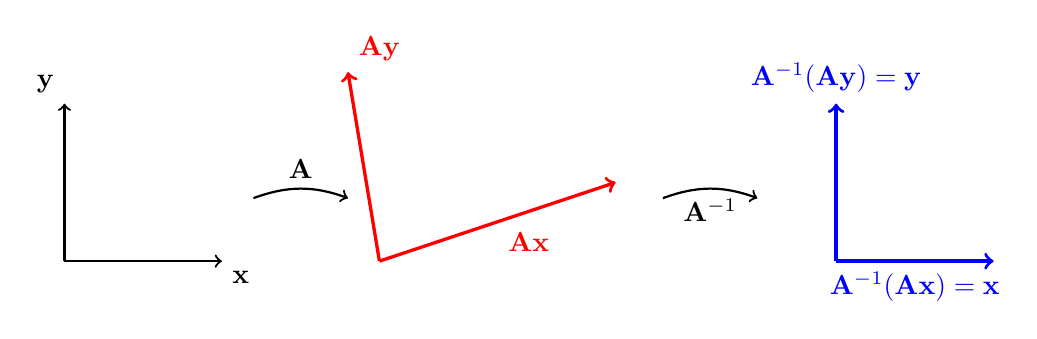
\begin{tikzpicture}[x=2cm,y=2cm]
 			
 			\begin{scope}
 				\draw[->, thick] (0,0) -- (1,0) node[below right] {${\bf x}$};
 				\draw[->, thick] (0,0) -- (0,1) node[above left] {${\bf y}$};
 			\end{scope}
 			
 			\begin{scope}[shift={(2.0,0)}]
 				\coordinate (A) at (1.5,0.5);
 				\coordinate (B) at (-0.2,1.2);
				\draw[->, very thick, red] (0,0) -- (A) node[pos=0.5, below right] {${\bf A}{\bf x}$};
 				\draw[->, very thick, red] (0,0) -- (B) node[above right] {${\bf A}{\bf y}$};
 			\end{scope}
 			
 			\begin{scope}[shift={(4.9,0)}]
 				\draw[->, very thick, blue] (0,0) -- (1,0) node[pos=0.5, below] {${\bf A}^{-1} ({\bf A}{\bf x}) = {\bf x}$};
 				\draw[->, very thick, blue] (0,0) -- (0,1) node[above] {${\bf A}^{-1} ({\bf A}{\bf y}) = {\bf y}$};
 			\end{scope}
 			
 			\draw[->, thick, bend left=20] (1.2,0.4) to node[above] {${\bf A}$} (1.8,0.4);
 			\draw[->, thick, bend left=20] (3.8,0.4) to node[below] {${\bf A}^{-1}$} (4.4,0.4);
 		\end{tikzpicture}
 		\caption{A matrix $\mathbf{A}$ represents a linear transformation of $\mathbb{R}^{2}$. The inverse matrix $\mathbf{A}^{-1}$ 
 			represents the inverse transformation. \label{fig_matrix_inverse_dict}} 
 		\end{figure}
		See also: matrix, determinant, linear regression, pseudoinverse.},
	first={inverse matrix},
		type=math,
	text={inverse matrix}
}

\newglossaryentry{matrix}
{name={matrix},
	description={A matrix\index{matrix} of size $m\times d$ is a 2-D array of numbers, 
 		which is denoted by 
		$$
  		{\bf A}= \begin{pmatrix}
   		A_{1,1} & A_{1,2} & \dots  & A_{1,d} \\
		A_{2,1} & A_{2,2} & \dots  & A_{2,d} \\
		\vdots  & \vdots  & \ddots & \vdots \\
		A_{m,1} & A_{m,2} & \dots  & A_{m,d}
		\end{pmatrix} \in \mathbb{R}^{m\times d}.
		$$
		Here, $A_{r,j}$ denotes the matrix entry in the $r$th row and the 
		$j$th column. Matrices are useful representations of various mathematical objects \cite{StrangLinAlg2016},
		including the following:
		\begin{itemize}
			\item Systems of linear equations: We can use a matrix to represent a system of linear equations 
			$$ \begin{pmatrix}
			A_{1,1} & A_{1,2} \\
			A_{2,1} & A_{2,2}
			\end{pmatrix}
			\begin{pmatrix}
				w_1 \\
				w_2
			\end{pmatrix}
			=\begin{pmatrix}
				y_1 \\
				y_2
			\end{pmatrix}
			\quad \text{ compactly as } \quad {\bf A}{\bf w}= {\bf y}.
			$$
    			One important example of systems of linear equations is the optimality condition for the 
    			model parameters within linear regression. 
			\item Linear maps:
			Consider a $d$-dimensional vector space $\mathcal{U}$ and a $m$-dimensional vector space $\mathcal{V}$. 
			If we fix a basis $\mathbf{u}^{(1)},\,\ldots,\,\mathbf{u}^{(d)}$ for $\mathcal{U}$ and a basis $\mathbf{v}^{(1)},\,\ldots,\,\mathbf{v}^{(m)}$ 
			for $\mathcal{V}$, each matrix ${\bf A}\in \mathbb{R}^{m\times d}$ naturally defines a 
			linear map $\alpha: \mathcal{U} \rightarrow \mathcal{V}$ (see Fig. \ref{fig_matrix_dict}) such that
   			$${\bf u}^{(j)} \mapsto \sum_{r=1}^{m} A_{r,j} {\bf v}^{(r)}.$$
			\item Datasets: We can use a matrix to represent a dataset. Each row 
			corresponds to a single data point, and each column corresponds to a specific 
			feature or label of a data point. 
		\end{itemize}
		\begin{figure}[H]
		\begin{center}
		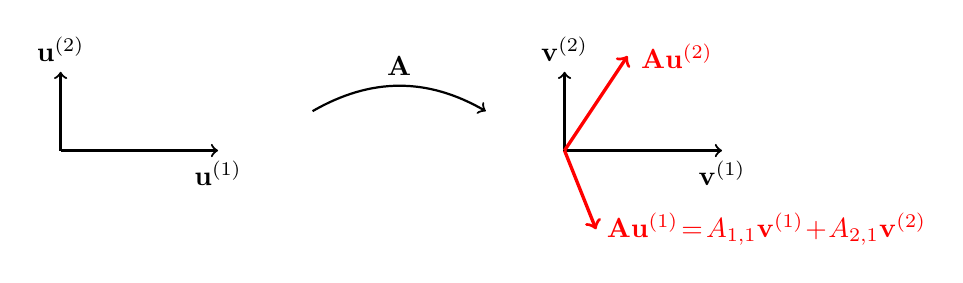
\begin{tikzpicture}[x=2cm]
			
			\begin{scope}
				\draw[->, thick] (0,0) -- (1,0) node[below] {${\bf u}^{(1)}$};
				\draw[->, thick] (0,0) -- (0,1) node[above] {${\bf u}^{(2)}$};
				
				
				
			\end{scope}
			
			\begin{scope}[shift={(3.2,0)}]
				\draw[->, thick] (0,0) -- (1,0) node[below] {${\bf v}^{(1)}$};
				\draw[->, thick] (0,0) -- (0,1) node[above] {${\bf v}^{(2)}$};
				\coordinate (A) at (0.2,-1.0);
				\coordinate (B) at (0.4,1.2);
				\draw[->, very thick, red] (0,0) -- (A) node[below,right] {${\bf A}{\bf u}^{(1)}\!=\!A_{1,1}{\bf v}^{(1)}\!+\!A_{2,1}{\bf v}^{(2)}$};
				\draw[->, very thick, red] (0,0) -- (B) node[right,xshift=1pt] {${\bf A}{\bf u}^{(2)}$};
				
				
			\end{scope}
			
			\draw[->, thick] (1.6,0.5) to[bend left] node[midway, above] {${\bf A}$} (2.7,0.5);
		
		\end{tikzpicture}
		\end{center}
		\caption{A matrix ${\bf A}$ defines a linear map between two vector spaces. \label{fig_matrix_dict}} 
		\end{figure}
		See also: linear map, dataset, linear model. },
	first={matrix},
	firstplural={matrices},
	type=math,
	plural={matrices},
	text={matrix}
}

\newglossaryentry{stratification}
{name={stratification},
 description={The process of splitting a dataset into subsets, so called strata,
 according to some key attribute is called stratification\index{stratification} \cite{oecd2008glossary,Everitt2010,OxfordStatisticsDictionary}. 
 The goal is to ensure that a machine learning (ML) method performs well for each stratum 
defined by these attributes. For example, in a medical dataset,
  we may want to stratify a patient dataset by age groups to ensure that an
  machine learning (ML) model performs well across all age groups.  
 \begin{figure}[H]
 	\centering
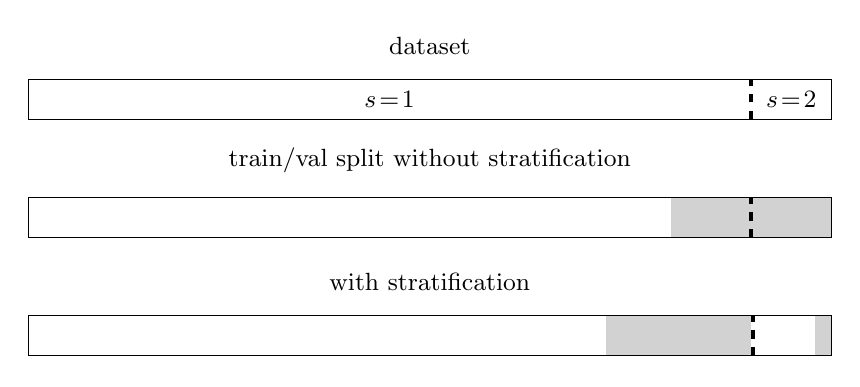
\begin{tikzpicture}[font=\small,x=1.7cm]
	
	\def\cellw{6.0}     
	\def\cellh{0.5}     
	\def\gap{1}       
	\def\tfrac{0.8}     
	\def\pA{0.9}        
	
	\node[anchor=south] at (0.5*\cellw, \cellh+0.2) {dataset};
	\node[anchor=south] at ({0.5*\cellw}, {-(\cellh+\gap)+\cellh+0.2}) {train/val split without stratification};
	\node[anchor=south] at (0.5*\cellw, {-2*(\cellh+\gap)+\cellh+0.2}) {with stratification};
	
	\pgfmathsetmacro{\yDataset}{0}
	\pgfmathsetmacro{\yNoStrat}{-(\cellh+\gap)}
	\pgfmathsetmacro{\yStrat}{-2*(\cellh+\gap)}
	
	\pgfmathsetmacro{\xAB}{\pA*\cellw}
	\pgfmathsetmacro{\wA}{\pA*\cellw}
	\pgfmathsetmacro{\wB}{(1-\pA)*\cellw}
	
	\draw (0,\yDataset) rectangle ++(\cellw,\cellh);
	\draw[dashed,  line width=0.5mm] (\xAB,\yDataset) -- ++(0,\cellh);
		
	\node at (0.5*\wA, \yDataset+0.5*\cellh) {$s\!=\!1$};
	\node at ({\xAB+0.5*\wB}, {\yDataset+0.5*\cellh}) {$s\!=\!2$};

	\draw (0,\yNoStrat) rectangle ++(\cellw,\cellh);
	\pgfmathsetmacro{\xValStart}{\tfrac*\cellw}
	\pgfmathsetmacro{\valw}{(1-\tfrac)*\cellw}
	\fill[gray!35] (\xValStart,\yNoStrat) rectangle ++(\valw,\cellh);


	\draw[dashed,  line width=0.5mm] (\xAB,\yNoStrat) -- ++(0,\cellh);
	
	\draw (0,\yStrat) rectangle ++(\cellw,\cellh);
	
	\pgfmathsetmacro{\xAB}{\pA*\cellw}
	\draw[dashed, line width=1mm] (\xAB,\yStrat) -- ++(0,\cellh);
	
	
	\pgfmathsetmacro{\xAVal}{\tfrac*\wA}              
	\pgfmathsetmacro{\wAVal}{(1-\tfrac)*\wA}          
	\fill[gray!35] (\xAVal,\yStrat) rectangle ++(\wAVal,\cellh);
	
	\pgfmathsetmacro{\xBVal}{\xAB + \tfrac*\wB}       
	\pgfmathsetmacro{\wBVal}{(1-\tfrac)*\wB}          
	\fill[gray!35] (\xBVal,\yStrat) rectangle ++(\wBVal,\cellh);
\end{tikzpicture}
 	\caption{Stratification ensures that both the training set and the validation set 
	(shaded grey) have similar 
 		distributions of a binary key attribute $s$.}
 \end{figure}
  When splitting a dataset into a training set and a validation set, 
  stratification ensures that both sets have similar distributions of the key attribute. 
  Without stratification, using a small validation set may underrepresent or 
  even completely miss data points with a rare attribute, leading to misleading 
  performance estimates.\\ 
  See also: validation, $k$-fold cross-validation ($k$-fold CV), stratum.},
  text={stratification},
  first={stratification},
  plural={stratifications}
}

\newglossaryentry{stratum}
{name={stratum},
	description={
	A\index{stratum} stratum is a subset of data points that all 
	possess a shared property (which could be a feature or a label). 
	For example, in a weather dataset, all measurements from the same 
	Finnish Meteorological Institute (FMI) weather station form one stratum.\\[0.5em]
	\begin{center}
\textbf{Example (CSV snippet):}\\
  {\ttfamily
  time,station,value,units\\
  2023-06-01 12:00,Helsinki,18.2,degC\\
  2023-06-01 13:00,Helsinki,18.5,degC\\
  2023-06-01 14:00,Helsinki,19.0,degC\\
  2023-06-01 12:00,Oulu,12.1,degC\\
  2023-06-01 13:00,Oulu,12.4,degC\\
  2023-06-01 14:00,Oulu,12.7,degC\\
  2023-06-01 12:00,Tampere,15.3,degC\\
  2023-06-01 13:00,Tampere,15.6,degC\\
  2023-06-01 14:00,Tampere,16.0,degC
  }
	\end{center} 
	Here, the rows for each station (\texttt{Helsinki}, \texttt{Oulu}, \texttt{Tampere}) 
	represent different strata.\\ 
	See also: stratification, dataset, data point.},
  first={stratum},
  firstplural={strata},
 plural={strata}, 
 text={stratum}
}


\newglossaryentry{det}
{name={determinant},
	description={The\index{determinant} determinant $\det\,({\bf A})$ of a square matrix 
		${\bf A}=\linebreak \big( {\bf a}^{(1)},\,\ldots,\,{\bf a}^{(d)} \big) \in \mathbb{R}^{d\times d}$ is a 
		function of its columns ${\bf a}^{(1)},\,\ldots,\,{\bf a}^{(d)} \in \mathbb{R}^{d}$, i.e., it satisfies 
		the following properties \cite{DirschmidHansJorg1996TuF}:
		\begin{itemize}
			\item Normalized: $$\det\,(\mathbf{I}) = 1$$ 
			\item Multilinear: \begin{align} \nonumber \det \big({\bf a}^{(1)},\,\ldots,\,\alpha{\bf u}+ \beta {\bf v},\,\ldots,\,{\bf a}^{(d)} \big) & = \alpha\det \big({\bf a}^{(1)},\,\ldots,\,{\bf u},\,\ldots,\,{\bf a}^{(d)} \big) \\ 
			& +\beta\det \big({\bf a}^{(1)},\,\ldots,\,{\bf v},\,\ldots,\,{\bf a}^{(d)} \big) \nonumber
			\end{align}
			\item Antisymmetric: $$\det \big(\ldots,\,{\bf a}^{(j)}, \,\ldots, \,{\bf a}^{(j')},\,\ldots \big) = - \det \big(\ldots,\,{\bf a}^{(j')}, \,\ldots, \,{\bf a}^{(j)},\,\ldots \big).$$ 
		\end{itemize} 
		We can interpret a matrix ${\bf A}$ as a linear transformation on $\mathbb{R}^{d}$.
		The determinant $\det\,({\bf A})$ characterizes how volumes in $\mathbb{R}^d$ (and their orientation) 
		are altered by this transformation (see Fig. \ref{fig_det_dict}) \cite{GolubVanLoanBook}, \cite{Strang2007}. 
 		In particular, $\det\,({\bf A}) > 0$ preserves orientation, $\det\,({\bf A}) < 0$ reverses orientation, 
 		and $\det\,({\bf A}) = 0$ collapses volume entirely, indicating that ${\bf A}$ is non-invertible. 
 		The determinant also satisfies $\det\,({\bf A}{\bf B}) = \det\,({\bf A}) \cdot \det\,({\bf B})$, and if ${\bf A}$ is 
 		diagonalizable with eigenvalues $\lambda_{1}, \,\ldots, \,\lambda_{d}$, then 
		$\det\,({\bf A}) = \prod_{j=1}^{d} \lambda_{j}$ \cite{HornMatAnalysis}.
    		For the special cases $d=2$ (i.e., two-dimensional or 2-D) and $d=3$ (i.e., three-dimensional or 3-D), 
		the determinant can be interpreted as an oriented area or volume spanned by the column vectors of ${\bf A}$.
    		\begin{figure}[H]
    			\begin{center}
    			\begin{tikzpicture}[x=2cm]
			
			\begin{scope}
			\draw[->, thick] (0,0) -- (1,0) node[below right] {${\bf x}$};
			\draw[->, thick] (0,0) -- (0,1) node[above left] {${\bf y}$};
			
			
			
			\end{scope}
			
			\begin{scope}[shift={(2.8,0)}]
			\coordinate (A) at (1.5,0.5);
			\coordinate (B) at (-0.2,1.2);
			\draw[->, very thick, red] (0,0) -- (A) node[below right] {${\bf A}{\bf x}$};
			\draw[->, very thick, red] (0,0) -- (B) node[above left] {${\bf A}{\bf y}$};
			\draw[fill=red!20, opacity=0.6] (0,0) -- (A) -- ($(A)+(B)$) -- (B) -- cycle;
			\draw[dashed] (A) -- ($(A)+(B)$);
			\draw[dashed] (B) -- ($(A)+(B)$);
			\node at (0.8,0.6) {\small $\det\,({\bf A})$};
			
			\draw[->, thick, blue] (0.4,0.0) arc[start angle=0, end angle=35, radius=0.6];
			
			
			\end{scope}
			
			\draw[->, thick] (1.3,0.5) -- (2.4,0.5) node[midway, above] {${\bf A}$};
			\end{tikzpicture}
			\end{center}
			\caption{We can interpret a square matrix ${\bf A}$ as a linear transformation of $\mathbb{R}^{d}$ 
				into itself. The determinant $\det\,({\bf A})$ characterizes how this transformation alters an oriented volume.
				\label{fig_det_dict}}
		\end{figure}
		See also: eigenvalue, inverse matrix.},
	first={determinant},
	type=math,
	text={determinant}
}

\newglossaryentry{hessian}
{name={Hessian},
 	description={Consider\index{Hessian} a function 
	$f: \mathbb{R}^{d} \to \mathbb{R}$ for which the second-order 
	partial derivatives exist at ${\bf x}'$. Then, the Hessian $\nabla^2 f({\bf x}')$ 
	of $f$ at ${\bf x}$ is defined as the matrix of second-order 
	partial derivatives of $f$ at ${\bf x}'$, 
$$\nabla^{2} f({\bf x}') \;=\;
\begin{pmatrix}
\frac{\partial^{2} f}{\partial \feature_{1}^{2}}
& \frac{\partial^{2} f}{\partial \feature_{1}\, \partial \feature_{2}}
& \cdots
& \frac{\partial^{2} f}{\partial \feature_{1}\, \partial \feature_{d}} \\
\frac{\partial^{2} f}{\partial \feature_{2}\, \partial \feature_{1}}
& \frac{\partial^{2} f}{\partial \feature_{2}^{2}}
& \cdots
& \frac{\partial^{2} f}{\partial \feature_{2}\, \partial \feature_{d}} \\
\vdots & \vdots & \ddots & \vdots \\[1.2ex]
\frac{\partial^{2} f}{\partial \feature_{d}\, \partial \feature_{1}}
& \frac{\partial^{2} f}{\partial \feature_{d}\, \partial \feature_{2}}
& \cdots
& \frac{\partial^{2} f}{\partial \feature_{d}^{2}}
\end{pmatrix}.$$
If the second-order partial derivatives are continuous in a neighborhood around ${\bf x}'$, then the Hessian is a symmetric matrix, i.e.,
$\frac{\partial^{2} f}{\partial \feature_{j}\, \partial \feature_{j'}} = 
\frac{\partial^{2} f}{\partial \feature_{j'}\, \partial \feature_{j}}$ for all 
$j, j'$ \cite{RudinBookPrinciplesMatheAnalysis}. If additionally $f$ 
is convex, then the Hessian is a positive semi-definite (psd) matrix \cite{BoydConvexBook}.
	\begin{figure}[H]
	\begin{center}
	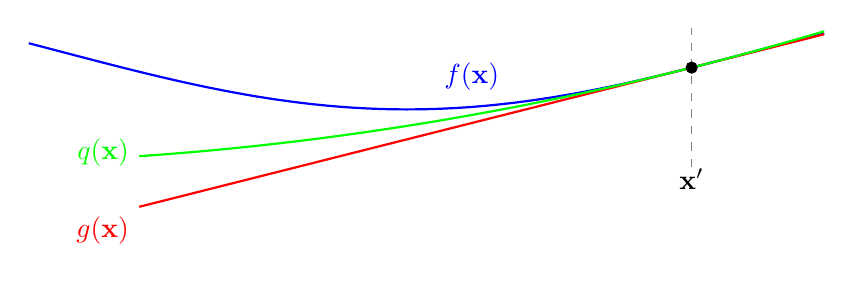
\begin{tikzpicture}[x=0.5cm]
		\begin{axis}[
			hide axis,
			xmin=3, xmax=6,
			ymin=0, ymax=6,
			domain=0:6,
			samples=100,
			width=10cm,
			height=6cm,
			clip=false
			]
		
			\addplot[blue, thick, domain=3:6.6] {2 + sin(deg(x))} 
			node[pos=0.5, above right, yshift=3pt] {$f({\bf x})$};
		
		
			\addplot[red, thick, domain=3.5:6.6] 
			{2 + sin(deg(6)) + cos(deg(6))*(x - 6)}
			node[pos=0, below left] {$g({\bf x})$};
                
                \addplot[green, thick, domain=3.5:6.6]
                {2 + sin(deg(6)) + cos(deg(6))*(x - 6) - 0.5*sin(deg(6))*(x - 6)^2}
			node[pos=0, below left, yshift=10pt] {$q({\bf x})$};
                
		
			\addplot[mark=*] coordinates {(6, {2 + sin(deg(6))})};
			    
			\addplot[dashed, gray] coordinates {(6,0) (6,2.4)};
			\node at (axis cs:6, -0.2) {${\bf x}'$};
			    
			    
			\pgfmathsetmacro{\xA}{-1.5}
			\pgfmathsetmacro{\xB}{3}
			\pgfmathsetmacro{\yA}{2 + sin(deg(\xA))}
			\pgfmathsetmacro{\yB}{2 + sin(deg(\xB))}
		\end{axis}
		\vspace*{-10mm}
	\end{tikzpicture}
		\vspace*{-5mm}
	\end{center}
	\caption{
		A function $f({\bf x})$ that is sufficiently smooth at a 
		point ${\bf x}'$ can be locally approximated by 
		a quadratic function $q({\bf x})$ which allows for a more accurate approximation 
		compared to a linear function $g({\bf x})$. \label{fig_quadapprox_hessian_dict}}
\end{figure}
		The Hessian $\nabla^2 f({\bf x}')$ can be used to compute a quadratic function 
		$$q({\bf x}) = (1/2) ({\bf x}- {\bf x}')^{T} \underbrace{\nabla^2 f({\bf x}')}_{\text{Hessian}} 
		({\bf x}- {\bf x}') +  ({\bf x}- {\bf x}')^{T} \underbrace{\nabla f({\bf x}')}_{\text{gradient}} 
		+ f({\bf x}')$$
		that approximates $f$ locally around ${\bf x}'$. 
        		\\
		See also: differentiable, matrix, function, quadratic function. }, 
	first={Hessian},
	type=math,
	text={Hessian}
}

\newglossaryentry{continuous}
{name={continuous}, 
description={A function\index{continuous} $f: \mathbb{R}^{d} \to \mathbb{R}$ is 
	 continuous at a point ${\bf x}' \in \mathbb{R}^{d}$ if for 
	 every $\epsilon > 0$ there is a $\delta > 0$ such that for all 
	 ${\bf x}\in \mathbb{R}^{d}$ with $\mleft\lVert {\bf x}- {\bf x}' \mright\rVert_{2} < \delta$, 
	 it holds that $|f({\bf x}) - f({\bf x}')| < \epsilon$ \cite{RudinBookPrinciplesMatheAnalysis}. 
	 In other words, we can make $f({\bf x})$ arbitrarily close to $f({\bf x}')$ 
	 by choosing ${\bf x}$ sufficiently close to ${\bf x}'$. If $f$ is continuous 
	 at every point ${\bf x}' \in \mathbb{R}^{d}$, then $f$ is said to be 
	 continuous on $\mathbb{R}^{d}$. The notion of a continuous 
	 function can be naturally extended to functions between general metric 
	 spaces \cite{RudinBookPrinciplesMatheAnalysis}.\\
		See also: Euclidean space, metric.},
	first={continuous},
	type=math,
	text={continuous}
}

\newglossaryentry{linearmap}
{name={linear map}, plural={linear maps}, 
	description={A\index{linear map} linear map $f: \mathbb{R}^n \rightarrow \mathbb{R}^m$ is a function that satisfies additivity, i.e.,
		$f({\bf x}+ {\bf y}) = f({\bf x}) + f({\bf y})$, and homogeneity, i.e.,
		$f(c{\bf x}) = c f({\bf x})$, for all vectors ${\bf x}, {\bf y}\in \mathbb{R}^n$ and scalars $c \in \mathbb{R}$. 
		In particular, $f(\mathbf{0}) = \mathbf{0}$. Any linear map can be represented as a matrix 
		multiplication $f({\bf x}) = {\bf A}{\bf x}$ for some matrix ${\bf A}\in \mathbb{R}^{m \times n}$. 
		The collection of real-valued linear maps for a given dimension $n$ constitute a linear model, 
		which is used in many machine learning (ML) methods.
		\\
		See also: map, function, vector, matrix, linear model, machine learning (ML).},
	first={linear map},
	text={linear map}
}

\newglossaryentry{vector}
{name={vector},
	description={A\index{vector} vector is an element of a vector space. 
		In the context of machine learning (ML), a particularly important example of a vector space 
		is the Euclidean space $\mathbb{R}^{d}$, where $d\in \mathbb{N}$ 
		is the (finite) dimension of the space. A vector ${\bf x}\in \mathbb{R}^{d}$ 
		can be represented as a list or one-dimensional (1-D) array of real numbers, i.e., 
		$x_1, \,\ldots, \,x_{d}$ with $x_j\in \mathbb{R}$ for 
		$j= 1, \,\ldots, \,d$. The value $x_j$ is the $j$th 
		entry of the vector ${\bf x}$. It can also be useful to view a vector ${\bf x}\in \mathbb{R}^{d}$ 
		as a function that maps each index $j\in \{1, \,\ldots, \,d\}$ 
		to a value $x_j\in \mathbb{R}$, i.e., ${\bf x}: j\mapsto x_j$. 
		This perspective is particularly useful for the study of kernel methods. See Fig. 
		\ref{fig:vector-function-dual_dict} for the two views of a vector.
		\begin{figure}[H]
			
			\begin{minipage}[c]{0.48\textwidth}
				\centering 
				2, --1, 3, 0, --2, 1
				\begin{minipage}{\textwidth}
				\vspace{5ex}
				\centering
				{\selectfont (a)}
				\end{minipage}
			\end{minipage}
			\hfill
			
			\begin{minipage}{0.48\textwidth}
			\centering
			\begin{tikzpicture}
			\begin{axis}[
    				width=6.5cm,
    				height=5cm,
    				title={},
    				xlabel={index $j$},
    				ylabel={$x_j$},
   		 		ymin=-3.5, ymax=3.5,
    				xmin=0.5, xmax=6.5,
   	 			xtick={1,2,3,4,5,6},
    				ytick={-3,-2,-1,0,1,2,3},
    				axis x line=bottom,        
    				axis y line=left,          
    				grid=both,
    				major grid style={dotted, gray!60},
    				enlargelimits=0.1
			]
			\addplot+[ycomb, thick, mark=*]
    			coordinates {
        				(1,2)
        				(2,-1)
       	 			(3,3)
        				(4,0)
        				(5,-2)
        				(6,1)
    			};
			\end{axis}
			\node at (2,-2.5) {(b)};
			\end{tikzpicture}
			\end{minipage}
			\caption{Two equivalent views of a vector ${\bf x}= \big( 2, -1, 3, 0, -2, 1 \big)^{T} \in \mathbb{R}^{6}$.
			(a) As a numeric array. (b) As a map $j\mapsto x_j$.}
			\label{fig:vector-function-dual_dict}
		\end{figure}
		See also: vector space, Euclidean space, linear map.},
	first={vector},
	firstplural={vectors},
	type=math,
	plural={vectors},
	text={vector}
}


\newglossaryentry{vectorspace}
{name={vector space},
	description={A\index{vector space} vector space $\mathcal{V}$ (also called linear space) 
		is a collection of elements, called vectors, along with the following two operations 
		(see also Fig. \ref{fig:vector-ops_dict}): 
    		1) addition (denoted by ${\bf v}+{\bf w}$) of two vectors ${\bf v},{\bf w}$; and 2) multiplication 
		(denoted by $c \,\cdot \,{\bf v}$) of a vector ${\bf v}$ with a scalar $c$ that belongs to some 
		number field (with a typical choice for this field being $\mathbb{R}$). The defining 
		property of a vector space is that it is closed under two specific operations. First, 
		if ${\bf v}, {\bf w}\in \mathcal{V}$, then ${\bf v}+ {\bf w}\in \mathcal{V}$. Second, if ${\bf v}\in \mathcal{V}$ 
		and $c \in \mathbb{R}$, then $c {\bf v}\in \mathcal{V}$.
		\begin{figure}[H]
		\centering
			\begin{tikzpicture}[>=Stealth, scale=1.2]
			
  			\coordinate (O) at (0,0);            
  			\coordinate (V) at (2,1.5);          
  			\coordinate (W) at (1,3);            
  			\coordinate (VplusW) at (3,4.5);     
  			\coordinate (HalfV) at (1,0.75);     
  			\draw[->, thick, blue] (O) -- (V) node[pos=1, right] {${\bf v}$};
  			\draw[->, thick, red] (O) -- (W) node[pos=1, left] {${\bf w}$};
  			\draw[->, thick, purple] (O) -- (VplusW) node[pos=0.99, above right] {${\bf v}+{\bf w}$};
  			\draw[dashed, red] (V) -- (VplusW);
  			\draw[dashed, blue] (W) -- (VplusW);
  			\draw[->, thick, orange] (O) -- (HalfV) node[midway, right] {$ \alpha {\bf v}$};
			
  			\filldraw[black] (O) circle (2pt) node[below left] {$\mathbf{0}$};  
  			\filldraw[blue] (V) circle (2pt);         
  			\filldraw[red] (W) circle (2pt);          
  			\filldraw[purple] (VplusW) circle (2pt);  
  			\filldraw[orange] (HalfV) circle (2pt);   
			\end{tikzpicture}
			\caption{A vector space $\mathcal{V}$ is a collection of vectors such that 
			scaling and adding them always yields another vector in $\mathcal{V}$.}
			
			
			\label{fig:vector-ops_dict}
		\end{figure}
		A common example of a vector space is the Euclidean space $\mathbb{R}^n$, which is 
		widely used in machine learning (ML) to represent datasets. We can also use $\mathbb{R}^n$ 
		to represent, either exactly or approximately, the hypothesis space used by an machine learning (ML) method.  
		Another example of a vector space, which is naturally associated with every probability space 
		$\big(\Omega,\mathcal{F},\mathbb{P}\left(\cdot\right) \big)$, is the collection of all 
		real-valued random variables (RVs) $x: \Omega\rightarrow \mathbb{R}$ \cite{RudinBook}, \cite{folland1999real}.  
		\\
		See also: vector, Euclidean space, linear model, linear map.},
	first={vector space},
	type=math,
	text={vector space}
}


\newglossaryentry{stochastic}
{name={stochastic},
	description={We refer to a \index{stochastic} method as stochastic if it involves a 
		random component or is governed by probabilistic laws. Machine learning (ML) methods use randomness 
		to reduce computational complexity (e.g., see stochastic gradient descent (SGD)) or 
		to capture uncertainty in probabilistic models.
		\\
		See also: stochastic gradient descent (SGD), uncertainty, probabilistic model.},
	first={stochastic},
	text={stochastic}
}

\newglossaryentry{stochproc}
{name={stochastic process},
	description={A stochastic process\index{stochastic process} is a collection of 
		random variables (RVs) defined on a common probability space and indexed by some set 
		$\mathcal{I}$ \cite{GrayProbBook}, \cite{papoulis}, \cite{Brockwell91}. The index set 
		$\mathcal{I}$ typically represents time or space, allowing us to represent 
		random phenomena that evolve across time or spatial dimensions—for example, 
		sensor noise or financial time series. Stochastic processes are not limited 
		to temporal or spatial settings. For instance, random graphs such as 
		the Erd\H{o}s–R\'enyi (ER) graph or the stochastic block model (SBM) can also be viewed as stochastic processes. 
		Here, the index set $\mathcal{I}$ consists of node pairs that index random variables (RVs) whose values 
		encode the presence or weight of an edge between two nodes. Moreover, stochastic 
		processes naturally arise in the analysis of stochastic algorithms, 
		such as stochastic gradient descent (SGD), which construct a sequence of random variables (RVs). 
		\\
		See also:  random variable (RV), stochastic block model (SBM), stochastic gradient descent (SGD), uncertainty, probabilistic model.},
	first={stochastic process},
	firstplural={stochastic processes},
	type=math, 
	plural={stochastic processes},
	text={stochastic process}
}

\newglossaryentry{characteristicfunc}
{name={characteristic function},
	description={The characteristic function\index{characteristic function} 
		of a real-valued random variable (RV) $x$ is the function \cite[Sec. 26]{BillingsleyProbMeasure}
		$$ \phi_{x}(t) :=\mathbb{E} { \exp\,(j t x) } \mbox{ with } j = \sqrt{-1}.$$
	 	The characteristic function uniquely determines the probability distribution of $x$. 
		\\
		See also: random variable (RV), probability distribution.},
	first={characteristic function},
	firstplural={characteristic functions}, 
	type=math, 
	plural={characteristic functions},
	text={characteristic function}
}

\newglossaryentry{entropy}
{name={entropy},
	description={Entropy\index{entropy} quantifies the uncertainty or unpredictability associated with a random variable (RV) \cite{coverthomas}. 
		For a discrete random variable (RV) $x$ taking on values in a finite set $\mathcal{S} = \{x_1, \,\ldots, \,x_n\}$ with 
		a probability mass function $p_i :=\mathbb{P}\left(x = x_i\right)$, the entropy is defined as
		\[
		H(x) :=-\sum_{i=1}^n p_i \log p_i.
		\]
		Entropy is maximized when all outcomes are equally likely, and minimized (i.e., zero) 
		when the outcome is deterministic. A generalization of the concept of entropy for continuous 
		random variables (RVs) is differential entropy. 
		\\
		See also: uncertainty, probabilistic model.},
	first={entropy},
	text={entropy}
}

\newglossaryentry{diffentropy}
{name={differential entropy},
	description={For\index{differential entropy} a real-valued random variable (RV) ${\bf x}\in \mathbb{R}^{d}$ 
		with a probability density function (pdf) $p(x)$, the differential entropy is defined as \cite{coverthomas}
		\[
		h({\bf x}) :=- \int p({\bf x}) \log p({\bf x}) \, d{\bf x}.
		\]
		Differential entropy can be negative and lacks some properties of entropy for 
		discrete-valued random variables (RVs), such as invariance under a change of variables \cite{coverthomas}. 
		Among all random variables (RVs) with a given mean ${\bm \mu}$ and covariance matrix ${\bf C}$, 
		$h({\bf x})$ is maximized by ${\bf x}\sim \mathcal{N}\left({\bm \mu},{\bf C}\right)$. 
		\\
		See also: uncertainty, probabilistic model.},
	first={differential entropy},
	text={differential entropy}
}

\newglossaryentry{minimum}
{name={minimum},
	description={Given a set of real numbers, the minimum\index{minimum} is the smallest of those numbers.
		Note that for some sets, such as the set of negative real numbers, the minimum does not exist.},
	firstplural={minima}, 
 	plural={minima},
	first={minimum},
	text={minimum}
}


\newglossaryentry{co-domain}
{name={co-domain}, 
	description={The co-domain\index{co-domain} of a function 
	$f: \mathcal{U} \rightarrow \mathcal{V}$ is the set $\mathcal{V}$ 
		into which $f$ maps elements of its domain $\mathcal{U}$.  
		\\
		See also: function, domain, map.},
	first={co-domain},
	firstplural={co-domains}, 
	type=math, 
	plural={co-domains},
	text={co-domain}
}

\newglossaryentry{domain}
{name={domain}, 
	description={The domain\index{domain} of a function 
	$f: \mathcal{U} \rightarrow \mathcal{V}$ is the set $\mathcal{U}$ 
		from which $f$ takes its inputs.  
		\\
		See also: function, co-domain, map.},
	first={domain},
	firstplural={domains}, 
	type=math, 
	plural={domains},
	text={domain}
}	
	

\newglossaryentry{function}
{name={function}, 
	description={A function\index{function} between two sets $\mathcal{U}$ and $\mathcal{V}$ assigns  
		each element $u \in \mathcal{U}$ exactly one element $f(u) \in \mathcal{V}$ \cite{RudinBookPrinciplesMatheAnalysis}.
		We write this as $$f: \mathcal{U} \rightarrow \mathcal{V}: u \mapsto f(u)$$ 
		where $\mathcal{U}$ is the domain and $\mathcal{V}$ the co-domain of $f$. 
		That is, a function $f$ defines a unique output $f(u) \in \mathcal{V}$ for every 
		input $u \in \mathcal{U}$ (see Fig. \ref{fig_function_dict}).
		\begin{figure}[H]
			\centering
			\begin{tikzpicture}[>=stealth, node distance=1.2cm and 2.5cm]
				\tikzset{dot/.style={circle, fill=black, inner sep=1.2pt}}
				\node (A) [dot, label=left:$a$] {};
				\node (B) [dot, below=of A, label=left:$b$] {};
				\node (C) [dot, below=of B, label=left:$c$] {};
				\node (1) [dot, right=4cm of A, label=right:$\star$] {};
				\node (2) [dot, below=of 1, label=right:$\circ$] {};
				\node (3) [dot, below=of 2, label=right:$\otimes$] {};
				\node[draw=blue!70, thick, ellipse, inner sep=0.5cm, fit=(A)(B)(C), label=above:$\mathcal{U}$] {};
				\node[draw=green!70!black, thick, ellipse, inner sep=0.5cm, fit=(1)(2)(3), label=above:$\mathcal{V}$] {};
				\draw[->] (A) -- (2);
				\draw[->] (B) -- (1);
				\draw[->] (C) -- (2);
			\end{tikzpicture}
			\caption{A function \( f \colon \mathcal{U} \to \mathcal{V} \) mapping each element 
			of the domain $\mathcal{U} =  \{a,b,c\}$ to exactly one element of 
				the co-domain $\mathcal{V} = \{\star,\circ,\otimes\}$. \label{fig_function_dict}}
		\end{figure} },
	first={function},
	firstplural={functions}, 
	type=math, 
	plural={functions},
	text={function}
}


\newglossaryentry{map}
{name={map}, 
	description={We\index{map} use the term map as a synonym for function.
		\\
		See also: function.},
	first={map},
	firstplural={maps},	
	type=math, 
	plural={maps},
	text={map}
}


\newglossaryentry{attention}
{name={attention}, 
	description={Some machine learning (ML) applications\index{attention} involve data points 
	composed of smaller units, referred to as tokens. For example, a sentence 
	consists of words, an image of pixel patches, and a network of nodes. In general, 
	the tokens that constitute a single data point are not independent 
	of one another. Instead, each token of a data point depends (or pays attention) 
	to specific other tokens. Probabilistic models provide a principled framework for 
	representing and analyzing such dependencies \cite{Blei2003}. Attention mechanisms use 
	a more direct approach without explicit reference to a probabilistic model. The idea is to 
		represent the relationship between two tokens $i$ and $i'$ using a parameterized function $f^{({\bf w})}(i,i')$, 
		where the parameters ${\bf w}$ are learned via a variant of empirical risk minimization (ERM). 
		Practical attention mechanisms differ in their precise choice of attention model $f^{({\bf w})}(i,i')$ 
		as well as in the precise empirical risk minimization (ERM) variant used to learn the parameters ${\bf w}$. One widely used family of attention mechanisms 
		defines the parameters ${\bf w}$ in terms of two vectors associated with each token $i$, i.e.,
		a query vector ${\bf q}^{(i)}$ and a key vector ${\bf k}^{(i')}$. For a given token $i$ 
		with query ${\bf q}^{(i)}$, and another token $i'$ with key ${\bf k}^{(i')}$, the quantity 
		$\big( {\bf q}^{(i)} \big)^{\top} {\bf k}^{(i')}$ quantifies the extent to which token $i$ attends 
		to (or depends on) token $i'$ (see Fig. \ref{fig_attention_dict}).
		\begin{figure}[H]
			\centering
			\begin{tikzpicture}[>=stealth, node distance=0.2cm and 0.2cm,
			every node/.style={inner sep=2pt, font=\large}, baseline]
			
			\node (w1) [draw, fill=gray!10, rounded corners] {All};
			\node (w2) [draw, fill=gray!10, right=of w1, rounded corners] {human};
			\node (w3) [draw, fill=gray!10, right=of w2, rounded corners] {beings};
			\node (w4) [draw, fill=gray!10, right=of w3, rounded corners] {are};
			\node (w5) [draw, fill=gray!10, right=of w4, rounded corners] {born};
			\node (w6) [draw, fill=gray!10, right=of w5, rounded corners] {free};
			\node (w7) [draw, fill=gray!10, right=of w6, rounded corners] {and};
			\node (w8) [draw, fill=blue!20, right=of w7, rounded corners] {equal};
			
   	   		\node[font=\footnotesize, below=0.15cm of w8, align=center] (labeli) {$i$ \\ ${\bf q}^{(i)},\ {\bf k}^{(i)}$};
			\node[font=\footnotesize, below=0.15cm of w1, align=center] (labelii) {$i'$ \\ ${\bf q}^{(i')},\ {\bf k}^{(i')}$};
			
	  		\node (eqTop) [above=1.8cm of w8] {};
	 		
	 		\draw[->, thick, opacity=0.3] (w8.north) .. controls +(up:1.0cm) and +(up:1.0cm) .. (w6.north); 
	 		\draw[->, thick, opacity=0.3] (w8.north) .. controls +(up:1.2cm) and +(up:1.0cm) .. (w5.north); 
			\draw[->, thick, opacity=1]  (w8.north)  .. controls +(up:1.8cm) and +(up:1.0cm) ..  node[midway, text=black, above] {$f^{({\bf w})}(i,i')$}  (w1.north); 
			\end{tikzpicture}
			\caption{Attention mechanisms learn a parameterized function $f^{({\bf w})}(i,i')$ to measure 
				how much token $i$ attends to token $i'$. One widely used construction of $f^{({\bf w})}(i,i')$ 
				uses query and key vectors, denoted by ${\bf q}^{(i)}$ and ${\bf k}^{(i)}$, assigned to each 
				token $i$ \cite{vaswani2017attention}. \label{fig_attention_dict}}
		\end{figure}
		See also: function, natural language processing (NLP), token.},
	first={attention},
	text={attention}
}

\newglossaryentry{transformer}
{name={transformer},
 description={In the context of machine learning (ML), the term transformer\index{transformer} 
 	refers to an ANNs that uses some form of attention mechanism 
 	to capture dependencies among tokens \cite{vaswani2017attention}. 
 	The attention mechansim is what sets transformers apart from 
	previous models used for sequential data such as recurrent neural network (RNN)s. 
	A transformer artificial neural network (ANN) often combines several attention layers 
	that are combined via more traditional layer architectures. \\ 
	See also: natural language processing (NLP), attention.
  }, 
 first = {transformer}, 
 text={transformer},
 firstplural={transformers}, 
 plural = {transformers}
}

\newglossaryentry{rnn}
{name={recurrent neural network (RNN)},
 description={A \index{recurrent neural network (RNN)} RNN 
  is a specific type of artificial neural network (ANN) that is designed for processing 
    data that consists of a sequence of tokens. 
	An RNN maintains an internal hidden state that is updated recurrently 
	as new tokens are processed. This recurrent dependence allows 
	information to propagate across time steps, making RNNs suitable for 
	tasks such as speech recognition, language modeling, or time series prediction. 
    However, their inherently sequential computation limits parallelization and 
	is challenging for gradient-based methods. Variants like the long short-term memory (LSTM) 
	and gated recurrent unit (GRU) mitigate these problems.}, 
 first = {recurrent neural network (RNN)},
 text={RNN}
}

\newglossaryentry{llm}
{name={large language model (LLM)},
 description={A\index{large language model (LLM)} LLM is an umbrella term for machine learning (ML) 
               methods that use high-dimensional machine learning (ML) models (with billions 
			   of model parameters) trained on large collections of text data. 
 			  LLMs are used to analyze or generate sequences of tokens which 
               constitute text data. Many current LLMs use some variant of 
			   a transformer that is trained via self-supervised learning:  
			   The training is based on the task of predicting a few words that 
			   are intentionally removed from a large text corpus. Thus, we can 
			   construct labeled data points simply by selecting some words 
			   from a given text as labels and the remaining words as features 
			   of data points. This construction requires 
		       very little human supervision and allows for generating sufficiently 
		       large training sets for LLMs.\\ 
			   See also: natural language processing (NLP), token, transformer.}, 
  first = {LLM}, 
  firstplural={LLMs}, 
  text = {LLM}, 
  plural = {LLMs} 
}


 \newglossaryentry{selfsupervisedlearning}
 {name={self-supervised learning},
  description={Self-supervised learning \index{self-supervised learning} uses some of 
  			   the features of a data point as its label. For 
			   example, if a data point consists of a sentence within a text document, 
			   we an use the last word of the sentence as the label which is 
			   to be predicted from all the previous words (which form the features 
			   of the data point). A main application of self-supervised learning 
			   is in natural language processing (NLP) for the training of LLMs from large collections 
			   of text data. \\ 
      See also: feature, label, LLM.}, 
   first = {self-supervised learning}, 
   text = {self-supervised learning}
}



\newglossaryentry{optproblem}
{name={optimization problem}, 
	description={An\index{optimization problem} optimization problem is a mathematical 
		   structure consisting of an objective function $f: \mathcal{U} \rightarrow \mathcal{V}$ 
		   defined over an optimization variable ${\bf w}\in \mathcal{U}$, together with a 
		   feasible set $\mathcal{W} \subseteq \mathcal{U}$. The co-domain $\mathcal{V}$ is 
		   assumed to be ordered, meaning that for any two elements $\mathbf{a}, \mathbf{b} \in \mathcal{V}$, 
		   we can determine whether $\mathbf{a} < \mathbf{b}$, $\mathbf{a} = \mathbf{b}$, 
		   or $\mathbf{a} > \mathbf{b}$. The goal of optimization is to find those values ${\bf w}\in \mathcal{W}$ 
		   for which the objective $f({\bf w})$ is extremal—i.e., minimal or maximal \cite{BoydConvexBook}, \cite{BertsekasNonLinProgr}, \cite{nesterov04}.
		   \\
		   See also: objective function.},
	first={optimization problem},
	firstplural={optimization problems}, 
	type=math,
	plural={optimization problems}, 
	text={optimization problem}
}

\newglossaryentry{optmethod}
{name={optimization method},
	description={An\index{optimization method} optimization method is an algorithm that 
		reads in a representation of an optimization problem and delivers an (approximate) solution 
		as its output \cite{BoydConvexBook}, \cite{BertsekasNonLinProgr}, \cite{nesterov04}.
		 \\
		 See also: algorithm, optimization problem.},
	first={optimization method},
	firstplural={optimization methods}, 
	plural={optimization methods}, 
	text={optimization method}
}

\newglossaryentry{convexopt}
{name={convex optimization},
 	description={
	Convex optimization\index{convex optimization} studies the 
	formulation, properties, and efficient solution methods for convex optimization problems \cite{BoydConvexBook}.  
	A convex optimization problem (defined on the Euclidean space $\mathbb{R}^{d}$) 
	consists of a convex objective function $f: \mathbb{R}^{d} \rightarrow \mathbb{R}$  
    and a convex constraint set $\mathcal{C}$ for the optimization variable ${\bf w}$.  
    It can be written compactly as \cite{BoydConvexBook}
	$$ \min_{{\bf w}\in \mathcal{C}}  f({\bf w}).$$ 
	Alternatively, a convex optimization problem can be expressed in 
	terms of convex constraint functions $g_1,\ldots,g_k$ as
	\begin{align} 
		\min_{{\bf w}\in \mathbb{R}^{d}} & f({\bf w})   \nonumber \\ 
		\mbox{s.t.} \quad & g_{r}({\bf w}) \leq 0, \quad r=1,\,\ldots,\,k. \label{equ_def_convx_opt_constr_dict}
	\end{align} 
	\begin{figure}
		\centering
	\begin{tikzpicture}[>=stealth, scale=1.0]
  
  \draw[->] (-3,0) -- (5.2,0) node[below] {${\bf c}$};
  \draw[->] (0,-0.2) -- (0,4.2) node[left] {$t$};
  
  \draw[thick, domain=-1:3, smooth, variable=\x, name path=boundary]
    plot ({\x},{exp(-\x)});
  
  \path[fill=gray!40, opacity=0.4]
    (-1,3) -- (-1,{exp(1)}) -- plot[domain=-1:3] ({\x},{exp(-\x)})
    -- (3,3) -- cycle;
  
  \fill (0,1) circle (1.6pt) node[left] {$f^{\ast}$};
  
  
  \draw[dashed, domain=-1:3, smooth, variable=\x]
    plot ({\x},{(2/exp(1)) - (1/exp(1))*\x}); 
   
  
  \fill (1,{1/exp(1)}) circle (1.2pt);
  
  \node at (2.6,2.5) {$\mathcal{A}$};
  \node [below,yshift=-3pt] at (0,-0.2) {$\mathbf{0}$};
  \end{tikzpicture}
  \caption{A convex optimization problem \eqref{equ_def_convx_opt_constr_dict} can be represented 
  by a set $\mathcal{A}$ that consists of objective values $t$ and constraint values 
  ${\bf c}=\big(c_{1},\ldots,c_{d}\big)^{T}$ that are achievable, i.e., 
  $f({\bf w}) \leq t, g_{1}({\bf w})\leq c_{1},\ldots, g_{k}({\bf w}) \leq c_{k}$ 
  by some ${\bf w}\in \mathbb{R}^{d}$. The optimal value $f^{\ast}$ of the 
  optimization problem is the smallest $t$ for which $(\mathbf{0},t) \in \mathcal{A}$. }
\end{figure}
	The formulation \eqref{equ_def_convx_opt_constr_dict} lends, in turn, to the 
	epigraph form of \cite[Sec 5.3]{BoydConvexBook} 
	$$\inf \big\{ t \in \mathbb{R} : (\mathbf{0}, t) \in \mathcal{A} \big\},$$ 
	with the set 
	\begin{align} 
	\mathcal{A} :=\big\{ ({\bf c},t) & \in \mathbb{R}^{d} \times \mathbb{R} : 
    f({\bf w}) \leq t, \, \nonumber \\ 
   &  g_{r}({\bf w}) \leq c_{r}, \,
    r= 1,\ldots,k, 
    \text{ for some } {\bf w}\in \mathbb{R}^{d} \big\}. \nonumber
	\end{align}
	It can be shown that, since $f,g_{1},\ldots,g_{k}$ are convex functions, 
    $\mathcal{A}$ is a convex set \cite[Ch.2]{BoydConvexBook}.
	The set $\mathcal{A}$ fully characterizes the optimization problem~\eqref{equ_def_convx_opt_constr_dict} 
	and can be interpreted as the epigraph of the objective function~$f$ restricted to the 
	feasible region defined by the constraint functions $g_1,\ldots,g_k$.\\ 
    See also: convex, optimization problem, optimization method.
  },
	first={convex optimization},
	type=math,
  	text={convex optimization}
}

\newglossaryentry{newtonmethod}
{name={Newton's method},
	description={Newton's method\index{Newton's method} is an iterative optimization method for finding 
	local minima or maxima of a differentiable objective function $f({\bf w})$. 
	Like gradient-based methods, Newton's method also 
		computes a new estimate $\widehat{{\bf w}}_{t+1}$ by optimizing a local approximation of $f({\bf w})$ around 
		the current estimate $\widehat{{\bf w}}_{t}$. In contrast to gradient-based methods, which use the gradient to build 
		a local linear approximation, Newton's method uses the Hessian matrix to build a local quadratic approximation. 
		In particular, starting from an initial estimate $\widehat{{\bf w}}_{0}$, Newton's method iteratively updates the estimate according to 
		\[
		\widehat{{\bf w}}_{t+1}= \widehat{{\bf w}}_{t}- \big( \nabla^2 f\big(\widehat{{\bf w}}_{t}\big) \big)^{-1} \nabla f\big( \widehat{{\bf w}}_{t} \big) \mbox{, for } t=0,\,1,\,\ldots.
		\]
		Here, $\nabla f\big(\widehat{{\bf w}}_{t} \big)$ is the gradient, and $\nabla^2 f({\bf w}^{(t)})$ is 
		the Hessian of the objective function $f$. Since using a quadratic function as local approximation is more accurate 
		than using a linear function (which is a special case of a quadratic function), Newton's method tends to 
		converge faster than gradient-based methods (see Fig. \ref{fig_newtonmethod_dict}). However, this faster convergence comes at the increased computational 
		complexity of the iterations. Indeed, each iteration of Newton's method requires the inversion of the Hessian. 
		\begin{figure}[H]
		\centering
		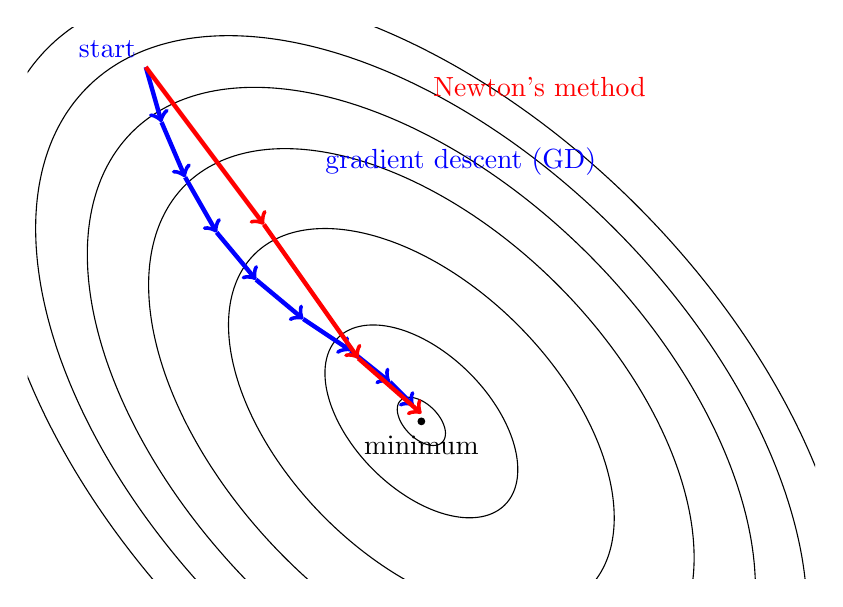
\begin{tikzpicture}[samples=200,smooth]
			\begin{scope}
				\clip(-5,-2) rectangle (5,5);
				\draw[thin] plot[domain=0:360] ({1.5*cos(\x)*sqrt(20/(sin(2*\x)+2))},{1.5*sin(\x)*sqrt(20/(sin(2*\x)+2))});
				\draw[thin] plot[domain=0:360] ({1.5*cos(\x)*sqrt(16/(sin(2*\x)+2))},{1.5*sin(\x)*sqrt(16/(sin(2*\x)+2))});
				\draw[thin] plot[domain=0:360] ({1.5*cos(\x)*sqrt(12/(sin(2*\x)+2))},{1.5*sin(\x)*sqrt(12/(sin(2*\x)+2))});
				\draw[thin] plot[domain=0:360] ({1.5*cos(\x)*sqrt(8/(sin(2*\x)+2))},{1.5*sin(\x)*sqrt(8/(sin(2*\x)+2))});
				\draw[thin] plot[domain=0:360] ({1.5*cos(\x)*sqrt(4/(sin(2*\x)+2))},{1.5*sin(\x)*sqrt(4/(sin(2*\x)+2))});
				\draw[thin] plot[domain=0:360] ({1.5*cos(\x)*sqrt(1/(sin(2*\x)+2))},{1.5*sin(\x)*sqrt(1/(sin(2*\x)+2))});
				\draw[thin] plot[domain=0:360] ({1.5*cos(\x)*sqrt(0.0625/(sin(2*\x)+2))},{1.5*sin(\x)*sqrt(0.0625/(sin(2*\x)+2))});
				
				\draw[->,blue,ultra thick] (-3.5,4.5) -- (-3.3,3.8);
				\draw[->,blue,ultra thick] (-3.3,3.8) -- (-3,3.1);
				\draw[->,blue,ultra thick] (-3,3.1) -- (-2.6,2.4);
				\draw[->,blue,ultra thick] (-2.6,2.4) -- (-2.1,1.8);
				\draw[->,blue,ultra thick] (-2.1,1.8) -- (-1.5,1.3);
				\draw[->,blue,ultra thick] (-1.5,1.3) -- (-0.9,0.9);
				\draw[->,blue,ultra thick] (-0.9,0.9) -- (-0.4,0.5);
				\draw[->,blue,ultra thick] (-0.4,0.5) -- (-0.1,0.2);
				\node[blue,above left] at (-3.5,4.5) {start};
				\node[blue,above] at (0.5,3) {gradient descent (GD)};
				
				\draw[->,red,ultra thick] (-3.5,4.5) -- (-2,2.5);
				\draw[->,red,ultra thick] (-2,2.5) -- (-0.8,0.8);
				\draw[->,red,ultra thick] (-0.8,0.8) -- (0,0.1);
				\node[red,above] at (1.5,4) {Newton's method};
				\node at (0,0) [circle,fill,inner sep=1pt,label=below:minimum] {};
			\end{scope}
		\end{tikzpicture}
		\caption{Comparison of gradient descent (GD) (blue) and Newton's method (red) paths toward the minimum of a 
			loss function. \label{fig_newtonmethod_dict}}
		\end{figure}
		See also: optimization method, gradient, Hessian, gradient descent (GD). },
  	first={newtonmethod},
 	type=math,
  	text={newtonmethod} 
}

\newglossaryentry{hilbertspace}
{name={Hilbert space},
 description={A \index{Hilbert space} Hilbert space $\mathcal{H}$ is a complete 
    inner product space. Thus, $\mathcal{H}$ is a vector space 
	equipped with an inner product $\langle \cdot, \cdot \rangle$. The inner product 
	induces a norm $\mleft\lVert \cdot \mright\rVert_{2}$ via $\mleft\lVert {\bf w}\mright\rVert_{2} = \sqrt{\langle {\bf w}, {\bf w}\rangle}$. 
  	Furthermore, $\mathcal{H}$ is complete in the sense that every 
 	Cauchy sequence $\big( {\bf w}^{(r)} \big)_{r\in \mathbb{N}}$ 
	in $\mathcal{H}$ converges to a limit $\lim_{r\rightarrow \infty} {\bf w}^{(r)}$ 
	that is also contained in $\mathcal{H}$. 
	\begin{figure}[H]
	\centering
	\begin{tikzpicture}[scale=3]
	
	
	
	
	\draw[gray!40] (0,0) circle (1);
	
	\def\ang{35} 
	
	\draw[->,thick] (0,0) -- (1,0) node[below right] {${\bf u}$};
	\draw[->,thick] (0,0) -- ({cos(\ang)},{sin(\ang)}) node[above] {${\bf v}$};
	
	\coordinate (P) at ({cos(\ang)},0);
	\draw[dashed] ({cos(\ang)},{sin(\ang)}) -- (P);
	\draw[->,thick] (0,0) -- (P) node[pos=0.5,below] {$\langle {\bf v}, {\bf u}\rangle {\bf u}$};
	
	\draw ($(P)+(0,0.06)$) -- (P) -- ($(P)+(-0.06,0)$);
	
	
	
	
	
	\node[right] at ({cos(-\ang)},{sin(-\ang)}) {$\mathbb{S}^{(d)} = \{ {\bf w}\in \mathbb{R}^{d}: \langle {\bf w}, {\bf w}\rangle=1\}$};
	
	
\end{tikzpicture}
\caption{For two unit-norm vectors ${\bf u}, {\bf v}\in \mathbb{S}^{(d)} \subseteq \mathbb{R}^{d}$ 
the inner product $\langle {\bf u}, {\bf v}\rangle$ is the expantion coefficient for the projection 
of ${\bf v}$ onto the subspace $\{ c {\bf u}: c \in \mathbb{R}\}$ spanned by ${\bf u}$. 
The absolute value $|\langle {\bf u}, {\bf v}\rangle|$ measures the norm of this projection.\label{fig_hilbertspace_dict}}
\end{figure}
	One important example of a Hilbert space 
 	is the Euclidean space $\mathbb{R}^{d}$ with the 
 	inner product $\langle {\bf w}, {\bf w}' \rangle = {\bf w}^{\top} {\bf w}'$ \\
   	See also: vector space.},
   	type=math, 
 	first = {Hilbert space}, 
    text = {Hilbert space},
   	plural={Hilbert spaces},
   	firstplural={Hilbert spaces}
  }

\newglossaryentry{cauchysequence}
{name={Cauchy sequence},
 description={A \index{Cauchy sequence} Cauchy sequence is a sequence
          $\big( {\bf x}^{(r)}\big)_{r\in \mathbb{N}}$ 
		  in a metric space $\left( \mathcal{X},d(\cdot,\cdot) \right)$ such 
		  that the elements ${\bf x}^{(r)}\in \mathcal{X}$ 
		  become arbitrarily close to each other eventually. 
		  In other words \cite[Def. 3.8.]{RudinBookPrinciplesMatheAnalysis}, 
		  \[
		  \forall \epsilon > 0, \exists N \in \mathbb{N} \text{ such that } 
		  \forall r, r' \geq N, \ d({\bf x}^{(r)},{\bf x}^{(r')}) < \epsilon.
		  \] 
		  \begin{figure}
			\centering
		  \begin{tikzpicture}[x=1cm,y=4cm]
			
					\def\srtwo{1.4142}
					\def\eps{0.15}
					\def\nmax{7}
			
			
			
			
						\fill[gray!30, opacity=0.35]
						(-0.3,{\srtwo-\eps}) rectangle (\nmax+0.6,{\srtwo+\eps});
					
					
					
				
				
				\draw[<->, thick] (4.5,{\srtwo-\eps}) -- (4.5,{\srtwo+\eps})
				node[above, right] {\footnotesize{$\varepsilon$}};
						
						\draw[dashed] (-0.3,\srtwo) -- (\nmax+0.6,\srtwo)
						node[right] {\footnotesize{$\sqrt{2}$}};
						
					      
					      \fill (0,1.0000) circle (1.2pt) node [right] {$x^{(1)}$};
					      \fill (1,1.5000) circle (1.2pt);
					      \fill (2,1.4167) circle (1.2pt);
					      \fill (3,1.4142) circle (1.2pt);
					      \fill (4,1.41421) circle (1.2pt);
					      \fill (5,1.4142136) circle (1.2pt);
					      \fill (6,1.41421356) circle (1.2pt);
			
						\def{\mathcal{N}}{1}
						\draw[densely dashed, thick, red] ({\mathcal{N}},0.88) -- ({\mathcal{N}},1.655);
						\node[right, red] at ({\mathcal{N}},0.8) {$N$};
						
						\node[align=right, anchor=north, font=\small]
						at (5,0.9)
						{\footnotesize{$\displaystyle x^{(r+1)}=\frac{1}{2}\!\left(x^{(r)}+\frac{2}{x^{(r)}}\right), x^{(1)}=1.$}};
						
			
			
			
			\end{tikzpicture}
			\caption{A Cauchy sequence 
			$\big(x^{(r)}\big)_{r\in\mathbb{N}}$ 
			in the metric space $\left( \mathbb{Q},|\cdot| \right)$. 
			This sequence is generated by a fixed-point iteration used to approximate 
			$\sqrt{2}$.  For all $r\ge N$, 
			the sequence elements lie within a band of width $\varepsilon$. 
			Note that the sequence does not converge in $\mathbb{Q}$ 
			since $\sqrt{2} \notin \mathbb{Q}$ \cite[Example 1.1.]{RudinBookPrinciplesMatheAnalysis}.\label{fig:fpit_cauchy_sqrt2_dict}}
			\end{figure}
		   Fig.\ \ref{fig:fpit_cauchy_sqrt2_dict} shows a Cauchy sequence in the metric space $\left( \mathbb{Q},|\cdot| \right)$ of 
		   rational numbers.  \\ 
		  See also: metric space, sequence. }, 
		type=math,
		first={Cauchy sequence},
		text={Cauchy sequence},
		plural={Cauchy sequences},
		firstplural={Cauchy sequences}
}

\newglossaryentry{nonexpansiveop}
 {name={non-expansive operator},
 	description={An \index{non-expansive operator} operator 
	$\mathcal{F}: \mathcal{H}\rightarrow \mathcal{H}$ defined on a 
	Hilbert space $\mathcal{H}$ is called non-expansive if it does 
	not increase distances. 
	In other words,  
 		\begin{equation} 
 			\nonumber
 			\mleft\lVert  \mathcal{F}{\bf w}- \mathcal{F}{\bf w}' \mright\rVert_{2} 
			\leq 	\mleft\lVert {\bf w}- {\bf w}' \mright\rVert_{2} \mbox{ for any } {\bf w}, {\bf w}' \in \mathcal{H}. 
 		\end{equation} 
 		See also: fixed-point iteration, contraction operator.},
 	type=math, 
	first={non-expansive operator},
 	plural={non-expansive operators},
	firstplural={non-expansive operators},
 	text={non-expansive operator}
 }

\newglossaryentry{fixedpointiter}
{name={fixed-point iteration},
	description={A\index{fixed-point iteration} fixed-point iteration is an iterative method 
	     for solving an optimization problem. It constructs a sequence ${\bf w}^{(0)}, \,{\bf w}^{(1)}, \,\ldots$ by 
		 repeatedly applying an operator $\mathcal{F}$, i.e., 
		 \begin{equation} 
		 	\label{equ_def_fixed_point_dict} 
		 	{\bf w}^{(t+1)} = \mathcal{F}{\bf w}^{(t)} \mbox{, for } t=0, \,1, \,\ldots.
		 \end{equation} 
		 The operator $\mathcal{F}$ is chosen such that any of its fixed points is a solution 
		 $\widehat{{\bf w}}$ to the given optimization problem. For example, given a differentiable and 
		 convex function $f({\bf w})$, the fixed points of the operator $\mathcal{F}: {\bf w}\mapsto {\bf w}- \nabla f({\bf w})$ 
		 coincide with the minimizers of $f({\bf w})$. In general, for a given optimization problem 
		 with solution $\widehat{{\bf w}}$, there are many different operators 
		 $\mathcal{F}$ whose fixed points are $\widehat{{\bf w}}$. Clearly, we should use an 
		 operator $\mathcal{F}$ in \eqref{equ_def_fixed_point_dict} that reduces the 
		 distance to a solution such that
		 \begin{equation} 
			\nonumber
			\underbrace{\mleft\lVert  {\bf w}^{(t+1)} - \widehat{{\bf w}} \mright\rVert_{2}}_{\stackrel{\eqref{equ_def_fixed_point_dict}}{=} \mleft\lVert  \mathcal{F}{\bf w}^{(t)} - \mathcal{F}\widehat{{\bf w}} \mright\rVert_{2}}  \leq 	\mleft\lVert  {\bf w}^{(t)} - \widehat{{\bf w}} \mright\rVert_{2}. 
		\end{equation}
		Thus, we require $\mathcal{F}$ to be at least a non-expansive operator, i.e., the iteration \eqref{equ_def_fixed_point_dict} 
		should not result in worse model parameters that have a larger distance to a solution $\widehat{{\bf w}}$. 
		Furthermore, each iteration \eqref{equ_def_fixed_point_dict} should also make some progress, i.e., 
		reduce the distance to a solution $\widehat{{\bf w}}$. This requirement can be made precise using 
		the notion of a contraction operator \cite{Bauschke:2017}, \cite{fixedpoinIsta}. 
		The operator $\mathcal{F}$ is a contraction operator if, for some $\kappa\in [0,1)$,
		\begin{equation} 
			\nonumber
			\mleft\lVert  \mathcal{F}{\bf w}\!-\!\mathcal{F}{\bf w}' \mright\rVert_{2}  \leq  \kappa\mleft\lVert {\bf w}\!-\!{\bf w}' \mright\rVert_{2} \mbox{ holds for any } {\bf w},{\bf w}'.
		\end{equation}
		For a contraction operator $\mathcal{F}$, the fixed-point iteration \eqref{equ_def_fixed_point_dict} generates 
		a sequence ${\bf w}^{(t)}$ that converges quite rapidly. In particular \cite[Th. 9.23]{RudinBookPrinciplesMatheAnalysis}, 
		\begin{equation} 
			\nonumber
			\mleft\lVert  {\bf w}^{(t)} - \widehat{{\bf w}} \mright\rVert_{2} \leq \kappa^{t} 	\mleft\lVert  {\bf w}^{(0)} - \widehat{{\bf w}} \mright\rVert_{2}. 
		\end{equation} 
		Here, $\mleft\lVert  {\bf w}^{(0)} - \widehat{{\bf w}} \mright\rVert_{2}$ is the distance between 
		the initialization ${\bf w}^{(0)}$ and the solution $\widehat{{\bf w}}$. 
		It turns out that a fixed-point iteration \eqref{equ_def_fixed_point_dict} with a firmly non-expansive 
		operator $\mathcal{F}$ is guaranteed to converge to a fixed-point of $\mathcal{F}$ \cite[Corollary 5.16]{Bauschke:2017}. 
		Fig. \ref{fig_examples_nonexp_dict} depicts examples of a firmly non-expansive operator, a non-expansive operator, 
		and a contraction operator. All of these operators are defined on the 1-D space $\mathbb{R}$. 
		Another example of a firmly non-expansive operator is the proximal operator of a convex function \cite{Bauschke:2017}, \cite{ProximalMethods}. 
		\definecolor{darkgreen}{rgb}{0.0, 0.5, 0.0}
		\begin{figure}[H]
			\begin{center} 
				\begin{tikzpicture}[scale=1.5]
					
					\draw[line width=1pt, ->] (-2,0) -- (2,0) node[right] {$w^{(t)}$};
					\draw[line width=1pt, ->] (0,-2) -- (0,2) node[above] {$w^{(t+1)}$};
					
					\node at (2.1,2.2) {$\mathcal{F}^{(3)}$};
					\node at (1.9,-1.5) {$\mathcal{F}^{(1)}$};
					\node at (1.5,1.2) {$\mathcal{F}^{(2)}$};
					
					\draw[dashed] (1,-2) -- (1,2); 
					\draw[dashed] (-2,1) -- (2,1); 
					\draw[dashed] (-2,-1) -- (2,-1); 
					\draw[dashed] (-1,-2) -- (-1,2); 
					\node[above,xshift=4pt,yshift=-1pt] at (1,0) {$1$};
					\node[above,xshift=8pt,yshift=-1pt] at (0,-1) {$-1$};
					
					\draw[line width=2,domain=-2:2,smooth,blue] plot(\x,{0.5*\x + 1});
					
					\draw[line width=2,domain=-2:2,smooth,red] plot(\x,{-\x});
					
					\draw[line width=2, domain=-2:-1,smooth,darkgreen] plot(\x,{-1});
					\draw[line width=2,domain=-1:1,smooth,darkgreen] plot(\x,{\x});
					\draw[line width=2,domain=1:2,smooth,darkgreen] plot(\x,{1});
				\end{tikzpicture}
			\end{center} 
			\caption{Example of a non-expansive operator $\mathcal{F}^{(1)}$, a firmly non-expansive operator $\mathcal{F}^{(2)}$, and 
				a contraction operator $\mathcal{F}^{(3)}$. \label{fig_examples_nonexp_dict}}
		\end{figure} 
		See also: optimization problem, differentiable, convex, function, model parameters, contraction operator, proximal operator.},
	first={fixed-point iteration},
	text={fixed-point iteration},
	type=math, 
	firstplural={fixed-point iterations}, 
	plural={fixed-point iterations}
}


\newglossaryentry{ergraph}
{name={Erd\H{o}s–R\'enyi graph (ER graph)},
	description={An ER graph\index{Erd\H{o}s–R\'enyi graph (ER graph)} is a probabilistic model for graphs defined over 
		a given node set $i=1, \,\ldots, \,n$. One way to define the ER graph is 
		via the collection of independent and identically distributed (i.i.d.) binary random variables (RVs) $b^{(\{i,i'\})} \in \{0,1\}$, 
		for each pair of different nodes $i, i'$. A specific realization  
		of an ER graph contains an edge $\{i,i'\}$ if and only if 
		$b^{(\{i,i'\})}=1$. The ER graph is parameterized by the 
		number $n$ of nodes and the probability $\mathbb{P}\left(b^{(\{i,i'\})}=1\right)$. 
		\\
		See also: graph, probabilistic model, independent and identically distributed (i.i.d.), random variable (RV), realization, probability.},
	first={Erd\H{o}s–R\'enyi (ER) graph},
	text={ER graph}
}

\newglossaryentry{attack}
{name={attack},  
	description={An attack\index{attack} on an machine learning (ML) system refers to an intentional action—either 
		active or passive—that compromises the system's integrity, availability, or confidentiality. 
		Active attacks involve perturbing components such as datasets (via data poisoning) 
		or communication links between devices within an machine learning (ML) application. Passive attacks, 
		such as privacy attacks, aim to infer sensitive attributes without modifying the system. 
		Depending on their goal, we distinguish among denial-of-service attacks, backdoor attacks, and privacy attacks.
		\\
		See also: data poisoning, privacy attack, sensitive attribute, denial-of-service attack, backdoor.},
	plural={attacks}, 
	first={attack},
	firstplural={attacks},
	text={attack}
}

\newglossaryentry{privattack}
{name={privacy attack},
	description={A privacy attack\index{privacy attack} on an machine learning (ML) system aims to infer 
		sensitive attributes of individuals by exploiting partial access to a trained machine learning (ML) model. 
		One form of a privacy attack is model inversion.\\
		See also: attack, sensitive attribute, model inversion, trustworthy artificial intelligence (trustworthy AI), general data protection regulation (GDPR).},
	plural={privacy attacks}, 
	first={privacy attack},
	firstplural={privacy attacks}, 
	text={privacy attack}
}

\newglossaryentry{epigraph}
{name={epigraph},
  description={The epigraph\index{epigraph} of a real-valued function $f : \mathbb{R}^n \to \mathbb{R} \cup \{+\infty\}$ 
  	is the set of points lying on or above its graph (see Fig. \ref{fig_epigraph_dict}), i.e., 
		\[
		\operatorname{epi}(f) = \left\{ (\mathbf{x}, t) \in \mathbb{R}^n \times \mathbb{R} \,\middle|\, f(\mathbf{x}) \leq t \right\}.
		\]
		A function is convex if and only if its epigraph is a convex set \cite{BoydConvexBook}, \cite{BertCvxAnalOpt}.
		\begin{figure}[H]
			\centering
			\begin{tikzpicture}[scale=1.0]
				\begin{axis}[
					axis lines = middle,
					xlabel = $x$,
					ylabel = {},
					xmin=-2, xmax=2,
					ymin=0, ymax=4.5,
					samples=100,
					domain=-1.5:1.5,
					thick,
					width=8cm,
					height=6cm,
					grid=none,
					axis on top,
					]
					
					\addplot [blue, thick, domain=-1.5:1.5] {x^2} node [pos=0.85, anchor=south west, xshift=5pt] {$f(x)$};
					
					\addplot [
					name path=f,
					draw=none,
					ytick=\empty,
					domain=-1.5:1.5,
					] {x^2};
					\path[name path=top] (axis cs:-1.5,4) -- (axis cs:1.5,4);
					\addplot [
					blue!20,
					opacity=0.6,
					draw=none,
					] fill between [
					of=f and top,
					soft clip={domain=-1.5:1.5},
					];
					    \node[font=\small] at (axis cs:-1.0,2.3) {$\operatorname{epi}(f)$};
				
				\end{axis}
			\end{tikzpicture}
			\caption{Epigraph of the function $f(x) = x^2$ (i.e., the shaded area). \label{fig_epigraph_dict}}
		\end{figure}
		See also: function, convex.},
	first={epigraph},
	text={epigraph},
	plural={epigraphs}
}


\newglossaryentry{nullspace}
{name={nullspace},
	description={The nullspace\index{nullspace} of a matrix ${\bf A}\in \mathbb{R}^{d' \times d}$, 
		denoted by ${\rm null}\left({\bf A}\right)$, is the set of all vectors $\mathbf{n} \in \mathbb{R}^d$ 
    		such that $${\bf A}\mathbf{n} = \mathbf{0}.$$ 
		Consider a feature learning method that uses the matrix ${\bf A}$ to transform 
		a feature vector $\mathbf{x} \in \mathbb{R}^{d}$ of a data point 
		into a new feature vector ${\bf z}= {\bf A}\mathbf{x} \in \mathbb{R}^{d'}$. 
		The nullspace ${\rm null}\left({\bf A}\right)$ characterizes all directions in the original 
    		feature space $\mathbb{R}^{d}$ along which the transformation 
		${\bf A}\mathbf{x}$ remains unchanged. In other words, adding any vector from 
		the nullspace to a feature vector ${\bf x}$ does not affect the transformed 
		representation ${\bf z}$. This property can be exploited to enforce invariances in the 
		predictions (computed from ${\bf A}\mathbf{x}$). Fig.\ \ref{fig:nullspace-rotation-dict} 
		illustrates one such invariance. It shows rotated versions of two handwritten digits, 
		which approximately lie along 1-D curves in the original feature space. 
		These curves are aligned with a direction vector $\mathbf{n} \in \mathbb{R}^{d}$. 
    		To ensure that the trained model is invariant to such rotations, we can 
		choose the transformation matrix ${\bf A}$ such that $\mathbf{n} \in {\rm null}\left({\bf A}\right)$. 
		This ensures that ${\bf A}\mathbf{x}$, and hence the resulting prediction, 
		is approximately insensitive to rotations of the input image.
		\begin{figure}[H]
      			\centering
      			\includegraphics[width=0.6\textwidth]{assets/pythonsnacks/nullspace/nullspace_0_1.png}
	  		\caption{
			Rotated handwritings of two different digits. The rotations are approximately 
			aligned along straight lines parallel to the vector $\mathbf{n}$. For a 
			binary classifier distinguishing between these digits, a natural choice is 
			a linear feature map ${\bf x}\mapsto \mathbf{A}{\bf x}$ with a 
			matrix ${\bf A}$ whose nullspace contains $\mathbf{n}$, i.e., $\mathbf{n} \in \mathrm{null}({\bf A})$.
                \label{fig:nullspace-rotation-dict}}	
	       	\end{figure}
		See also: matrix, feature map, feature learning. \\ 
		Python demo: \href{https://github.com/AaltoDictionaryofML/AaltoDictionaryofML.github.io/blob/main/assets/pythonsnacks/nullspace/nullspace.py}{click me}},
 	first={nullspace},
 	firstplural={nullspaces},
 	plural={nullspaces},
 	text={nullspace}
}


\newglossaryentry{maximum}
{name={maximum},
	description={The maximum\index{maximum} of a set $\mathcal{A} \subseteq \mathbb{R}$ 
     		of real numbers is the greatest element in that set, if such an element exists. A set $\mathcal{A}$ 
     		has a maximum if it is bounded above and attains its supremum (or least upper bound) \cite[Sec.~1.4]{RudinBookPrinciplesMatheAnalysis}.
				\\ 
		See also: supremum (or least upper bound).},
 	first={maximum},
 	firstplural={maxima},
 	plural={maxima},
 	text={maximum}
}

\newglossaryentry{supremum}
{name={supremum (or least upper bound)},
	description={The supremum\index{supremum (or least upper bound)} of a set of real numbers is 
		the smallest number that is greater than or equal to every element in the set. More formally, a 
		real number $a$ is the supremum of a set $\mathcal{A} \subseteq \mathbb{R}$ if: 1) $a$ 
		is an upper bound of $\mathcal{A}$; and 2) no number smaller than $a$ is an upper bound of $\mathcal{A}$. 
		Every non-empty set of real numbers that is bounded above has a supremum, even if it does 
		not contain its supremum as an element \cite[Sec.~1.4]{RudinBookPrinciplesMatheAnalysis}.},
	firstplural={suprema}, 
  	plural={suprema},
	first={supremum (or least upper bound)},
	text={supremum}
}

\newglossaryentry{discrepancy}
{name={discrepancy},
	description={Consider\index{discrepancy} an federated learning (FL) application with networked data 
		represented by an federated learning network (FL network). federated learning (FL) methods use a discrepancy measure 
		to compare hypothesis maps from local models at nodes $i,i'$, 
		connected by an edge in the federated learning network (FL network).
					\\ 
		See also: federated learning (FL), federated learning network (FL network), local model.},
	first={discrepancy},
	firstplural={discrepancies}, 
  	plural={discrepancies}, 
	text={discrepancy}
}

\newglossaryentry{FedRelax}
{name={federated relaxed (FedRelax)},
	description={An\index{federated relaxed (FedRelax)} federated learning (FL) distributed algorithm. 
		\\ 
		See also: federated learning (FL), distributed algorithm.},
	first={FedRelax},
	text={FedRelax}
} 

\newglossaryentry{fedavg}
{name={federated averaging (FedAvg)},
	description={FedAvg\index{federated averaging (FedAvg)} refers to a family of iterative federated learning (FL) algorithms. 
		It uses a server-client setting and alternates between clientwise local models 
		retraining, followed by the aggregation of updated model parameters at the server 
		\cite{pmlr-v54-mcmahan17a}. The local update at client $i=1, \,\ldots, \,n$ 
		at time $t$ starts from the current model parameters ${\bf w}^{(t)}$ provided 
		by the server and typically amounts to executing few iterations of stochastic gradient descent (SGD). After completing the local updates, they are aggregated 
		by the server (e.g., by averaging them). Fig. \ref{fig_single_iteration_fedavg_dict} illustrates the execution of a single 
		iteration of FedAvg. 
		\begin{figure}[H]
			\begin{center}
			\begin{tikzpicture}[>=Stealth, node distance=1cm and 1.5cm, every node/.style={font=\small}]
			
			\tikzstyle{server} = [circle, fill=black, minimum size=6pt, inner sep=0pt]
			\tikzstyle{client} = [circle, draw=black, minimum size=6pt, inner sep=0pt]
			
			\node (label1) at (0,3.5) {broadcast};
			\node[right=2.5cm of label1] (label2) {local update};
			\node[right=2.5cm of label2] (label3) {aggregate};
			
			\node[server] (s1) at (label1 |- 0,2.5) {};
			\node[client] (c1l) at ($(s1) + (-1cm,-1cm)$) {};
			\node[client] (c1r) at ($(s1) + (1cm,-1cm)$) {};
			\node[] (dots1) at ($(s1) + (0cm,-1cm)$) {\ldots};
			\draw[->] (s1) -- (c1l) node[midway,left] {${\bf w}^{(t)}$};
			\draw[->] (s1) -- (c1r) node[midway,right] {${\bf w}^{(t)}$};
			\draw[->] (s1) -- (dots1);
			
			\node[server] (s2) at (label2 |- 0,2.5) {};
			\node[client] (c2l) at ($(s2) + (-1cm,-1cm)$) {};
			\node[client] (c2r) at ($(s2) + (1cm,-1cm)$) {};
			\node[] (dots2) at ($(s2) + (0cm,-1cm)$) {\ldots};
			\node[below=0.2cm of c2l] {$\mathbf{w}^{(t,1)}$};
			\node[below=0.2cm of c2r] {$\mathbf{w}^{(t,n)}$};
			
			\node[server] (s3) at (label3 |- 0,2.5) {};
			\node[above=0.01cm of s3, yshift=-4pt] {${\bf w}^{(t+1)}$};
			\node[client] (c3l) at ($(s3) + (-1cm,-1cm)$) {};
			\node[client] (c3r) at ($(s3) + (1cm,-1cm)$) {};
			\node[] (dots3) at ($(s3) + (0cm,-1cm)$) {\ldots};
			\draw[->] (c3l) -- (s3) node[midway,left] {$\mathbf{w}^{(t,1)}$};
			\draw[->] (c3r) -- (s3)  node[midway,right] {$\mathbf{w}^{(t,n)}$};
			\draw[->] (dots3) -- (s3);
			\end{tikzpicture}
			\end{center}
			\caption{Illustration of a single iteration of FedAvg, which consists of broadcasting model parameters by the 
			server, performing local updates at clients, and aggregating the updates by the server. 
			\label{fig_single_iteration_fedavg_dict}} 
		\end{figure} 
		See also: federated learning (FL), algorithm, local model, stochastic gradient descent (SGD).},
	first={FedAvg},
	text={FedAvg}
} 

\newglossaryentry{FedGD}
{name={federated gradient descent (FedGD)},
	description={An\index{federated gradient descent (FedGD)} federated learning (FL) distributed algorithm that 
		can be implemented as message passing across an federated learning network (FL network). 
		\\ 
		See also: federated learning (FL), distributed algorithm, federated learning network (FL network), gradient step, gradient-based method.},
	first={FedGD},
	text={FedGD}
} 

\newglossaryentry{FedSGD}
{name={federated stochastic gradient descent (FedSGD)},
	description={An\index{federated stochastic gradient descent (FedSGD)} federated learning (FL) distributed algorithm that 
		can be implemented as message passing across an federated learning network (FL network). 
		\\ 
		See also: federated learning (FL), distributed algorithm, federated learning network (FL network), gradient step, gradient-based method, stochastic gradient descent (SGD).},
	first={FedSGD},
	text={FedSGD}
} 

\newglossaryentry{hfl}
{name={horizontal federated learning (HFL)},
	description={HFL\index{horizontal federated learning (HFL)} uses local datasets constitut\-ed by different
	   	data points but uses the same features to characterize them \cite{HFLChapter2020}.
		For example, weather forecasting uses a network of spatially distributed
		weather (observation) stations. Each weather station measures the
		same quantities, such as daily temperature, air pressure, and precipitation.
		However, different weather stations measure the characteristics or
		features of different spatiotemporal regions. Each spatiotemporal region 
		represents an individual data point, each characterized by the same features 
		(e.g., daily temperature or air pressure).\\
		See also: semi-supervised learning (SSL), federated learning (FL), vertical federated learning (VFL).},
	first={horizontal federated learning (HFL)},
	text={HFL}
} 

\newglossaryentry{dimred}
{name={dimensionality reduction},
	description={Dimensionality reduction\index{dimensionality reduction} refers 
		to methods that learn a transformation 
		$h: \mathbb{R}^{d} \rightarrow \mathbb{R}^{d'}$ 
		of a (typically large) set of raw features $\feature_{1}, \,\ldots, \,\feature_{d}$ 
		into a smaller set of informative features $z_{1}, \,\ldots, \,z_{d'}$. 
		Using a smaller set of features is beneficial in several ways: 
		\begin{itemize} 
			\item {Statistical benefit:} It typically reduces the risk of overfitting, as 
			reducing the number of features often reduces the effective dimension of a model. 
			\item {Computational benefit:} Using fewer features means less computation 
			for the training of machine learning (ML) models. As a case in point, linear regression methods 
			need to invert a matrix whose size is determined by the number of features. 
			\item {Visualization:} Dimensionality reduction is also instrumental for data visualization. 
			For example, we can learn a transformation that delivers two features $z_{1},z_{2}$, 
			which we can use, in turn, as the coordinates of a scatterplot. Fig.\ \ref{fig:dimred-scatter_dict} 
			depicts the scatterplot of handwritten digits that are placed 
			using transformed features. Here, the data points are 
			naturally represented by a large number of greyscale values (one value for each pixel).
		\end{itemize} 
		 \begin{figure}[H]
		 \centering
		 \begin{tikzpicture}[scale=1]	
		
		 	\draw[->] (-0.5,0) -- (5.5,0) node[right] {$z_1$};
		 	\draw[->] (0,-0.5) -- (0,4.5) node[above] {$z_2$};
		
		 	\foreach \x/\y/\label in {
  		 		1.2/0.5/3,
  		 		0.8/2.0/8,
  		 		2.5/1.8/1,
  		 		3.8/3.5/6,
  		 		4.2/0.7/9,
  		 		2.8/3.0/7,
  		 		1.5/3.8/2
		 	}{
  		 		\node[draw, minimum size=0.6cm, inner sep=0pt] at (\x,\y)
    	 		{\label};
		 	}
		 	\end{tikzpicture}
		 	\caption{Example of dimensionality reduction: High-dimensional image data 
			(e.g., high-resolution images of handwritten digits) embedded into 2-D using 
			learned features $(z_1, z_2)$ and visualized in a scatterplot.}
		 	\label{fig:dimred-scatter_dict}
		 \end{figure}
		See also: overfitting, effective dimension, model, scatterplot, principal component analysis (PCA), Johnson--Lindenstrauss (JL) lemma.}, 
	first={dimensionality reduction},
	text={dimensionality reduction}
} 


\newglossaryentry{diagnosis}
{name={diagnosis},
	description={Consider\index{diagnosis} an empirical risk minimization (ERM)-based method that resulted in a trained model 
	(or learned hypothesis) $\hat{h}\in \mathcal{H}$. We can diagnose the 
	method by comparing the training error $E_{t}$ with the validation error $E_{v}$ 
	incurred by $\hat{h}$ on the training set and the validation set. 
	\begin{figure}[htbp]
	\begin{center}
		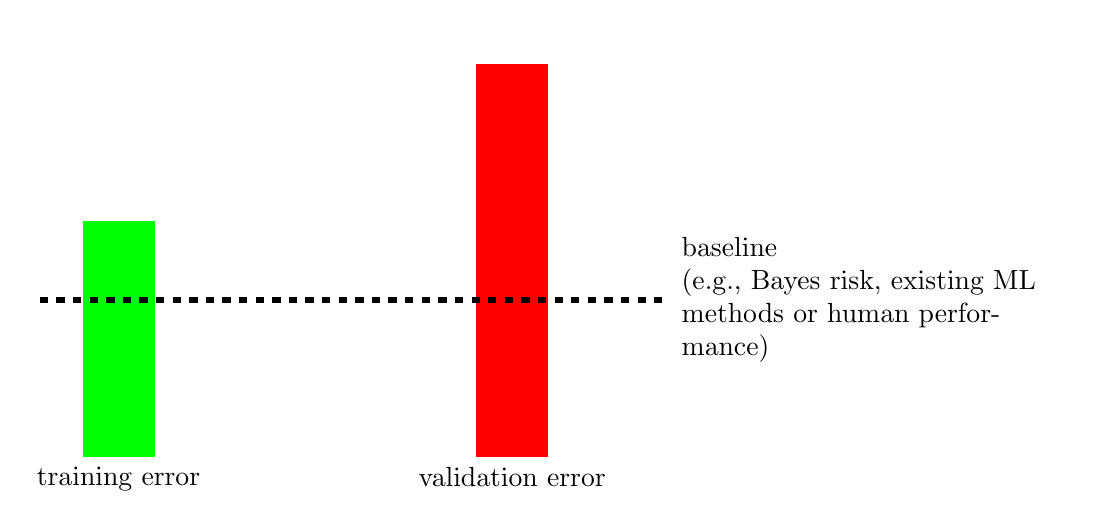
\begin{tikzpicture}[ycomb]
			\draw[color=green,line width=26pt]
			plot coordinates{(0,3)};
			\node [below] at (0,0) {training error} ; 
			\draw[color=red,line width=26pt]
			plot coordinates{(5,5)};
			\node [below] at (5,0) {validation error} ; 
			\draw[dashed,line width=2] (-1,2) -- (7,2) node[right,text width=5cm]{baseline \\ (e.g., Bayes risk, existing ML methods or human performance)};
		\end{tikzpicture}
	\end{center}
	\caption{We can diagnose a empirical risk minimization (ERM)-based machine learning (ML) method by comparing its training error 
		with its validation error. Ideally both are on the same level as a baseline.\label{fig_diagnosis_dict}}
		\end{figure}
	 			\\ 
		See also: validation, $k$-fold cross-validation ($k$-fold CV), generalization, baseline.},
	first={diagnosis},
	text={diagnosis}
} 


\newglossaryentry{ml}
{name={machine learning (ML)},
	description={ML\index{machine learning (ML)} aims to predict 
	 	a label from the features of a data point. ML methods achieve 
	 	this by learning a hypothesis from a hypothesis space (or model) 
	 	through the minimization of a loss function \cite{MLBasics}, \cite{HastieWainwrightBook}. 
	 	One precise formulation of this principle is empirical risk minimization (ERM). Different ML methods are 
	 	obtained from different design choices for data points (i.e., their features and label), 
	 	the model, and the loss function \cite[Ch. 3]{MLBasics}.
	 			\\ 
		See also: model, data, loss.},
	first={machine learning (ML)},
	text={ML}
} 


\newglossaryentry{reinforcementlearning}
{name={reinforcement learning (RL)},
	description={RL\index{reinforcement learning (RL)} refers to an online learning setting where 
		we can only evaluate the usefulness of a single hypothesis (i.e., a choice of model parameters) 
		at each time step $t$. In particular, RL methods apply the current hypothesis 
		$h^{(t)}$ to the feature vector ${\bf x}^{(t)}$ of the 
		newly received data point. The usefulness of the resulting prediction 
		$h^{(t)}({\bf x}^{(t)})$ is quantified by a reward 
		signal $r^{(t)}$ (see Fig. \ref{fig_reinforcementlearning_dict}). 
		\begin{figure}[H]
		\begin{center}
			\begin{tikzpicture}[scale=1]
			\draw[->] (-2, 0) -- (6, 0);
			\node at (6.3, 0) {$h$};
	        		
			\draw[thick, blue, domain=0:3, samples=20] plot (\x-3, {-0.2*(\x)^2 + 2});
			\node[anchor=west,yshift=4pt] at (0-3, {-0.2*(0)^2 + 2}) {$-L^{(t)}(h)$};
			
			\filldraw[blue] (1.5-3, {-0.2*(1.5)^2 + 2}) circle (2pt);
			\node[anchor=north] at (1.5-3, -0.3) {$h^{(t)}$};		
			\draw[dotted] (1.5-3, 0) -- (1.5-3, {-0.2*(1.5)^2 + 2});
			
			\draw[thick, red, domain=0:5, samples=20, dashed] plot (\x, {-0.15*(\x - 2)^2 + 3});
			\node[anchor=west,yshift=4pt] at (3, {-0.15*(3 - 2)^2 + 3}) {$-L^{(t+1)}(h)$};
			\filldraw[red] (2, {-0.15*(2 - 2)^2 + 3}) circle (2pt);
			\node[anchor=north] at (2, -0.3) {$h^{(t+1)}$};
			\draw[dotted] (2, 0) -- (2, {-0.15*(3 - 2)^2 + 3});
			
			\draw[thick, green!60!black, domain=3:5, samples=20, dotted] plot (\x+2, {-0.1*(\x - 4)^2 + 1.5});
			\node[anchor=west,yshift=4pt] at (4.5+2, {-0.1*(4.5 - 4)^2 + 1.5}) {$-L^{(t+2)}(h)$};
			\filldraw[green!60!black] (3.5+2, {-0.1*(3.5 - 4)^2 + 1.5}) circle (2pt);
			\node[anchor=north] at (3.5+2, -0.3) {$h^{(t+2)}$};
			\draw[dotted] (3.5+2, 0) -- (3.5+2, {-0.1*(3.5 - 4)^2 + 1.5});
			\end{tikzpicture}
		\caption{Three consecutive time steps $t,t+1,t+2$ with corresponding loss functions $L^{(t)},
		L^{(t+1)}, L^{(t+2)}$. During time step $t$, an RL method can evaluate the 
		loss function only for one specific hypothesis $h^{(t)}$, resulting in the reward 
		signal $r^{(t)}=-L^{(t)}(h^{(t)})$. \label{fig_reinforcementlearning_dict}}
		\end{center}
		\end{figure}
		In general, the reward depends also on the 
		previous predictions $h^{(t')}\big({\bf x}^{(t')}\big)$ 
		for $t' < t$. The goal of RL is to learn $h^{(t)}$, for 
		each time step $t$, such that the (possibly discounted) cumulative reward 
		is maximized \cite{MLBasics}, \cite{SuttonEd2}.
		\\
		See also: reward, loss function, machine learning (ML).},
	first={reinforcement learning (RL)},
	text={RL}
}


\newglossaryentry{featlearn}
{name={feature learning},
	description={Consider an machine learning (ML) application with data points characterized by 
		raw features ${\bf x}\in \mathcal{X}$. Feature learning\index{feature learning} 
		refers to the task of learning a map 
		$${\bf \Phi}: \mathcal{X}\rightarrow \mathcal{X}': {\bf x}\mapsto {\bf x}'$$ 
		that reads in the features ${\bf x}\in \mathcal{X}$ of a data point and delivers new 
		features ${\bf x}' \in \mathcal{X}'$ from a new feature space $\mathcal{X}'$. 
		Different feature learning methods are obtained for different design 
		choices of $\mathcal{X},\mathcal{X}'$, for a hypothesis space $\mathcal{H}$ 
		of potential maps ${\bf \Phi}$, and for a quantitative measure of the usefulness of 
		a specific ${\bf \Phi}\in \mathcal{H}$. For example, principal component analysis (PCA) 
		uses $\mathcal{X}:=\mathbb{R}^{d}$, $\mathcal{X}' :=\mathbb{R}^{d'}$ 
		with $d' < d$, and a hypothesis space 
		$$\mathcal{H}:=\big\{ {\bf \Phi}: \mathbb{R}^{d}
		\!\rightarrow\! \mathbb{R}^{d'}\!:\!{\bf x}'\!:=\!\mathbf{F}{\bf x}\mbox{ with some } \mathbf{F}\!\in\! \mathbb{R}^{d' \!\times d} \big\}.$$ Principal component analysis (PCA) measures the usefulness of a specific map ${\bf \Phi}({\bf x})= \mathbf{F}{\bf x}$ 
	by the minimum linear reconstruction error incurred on a dataset such that 
$$\min_{\mathbf{G}\in \mathbb{R}^{d\!\!\!\times d'}} \sum_{r=1}^{m} \mleft\lVert \mathbf{G}\mathbf{F}{\bf x}^{(r)} - {\bf x}^{(r)} \mright\rVert_{2}^{2}.$$ 
			\\ 
		See also: feature, feature space, hypothesis space, principal component analysis (PCA).}, 
	first={feature learning},
	text={feature learning}
} 

\newglossaryentry{autoencoder}
{name={autoencoder},
	description={An autoencoder\index{autoencoder} is an machine learning (ML) method that simultaneously 
		learns an encoder map $h\in \mathcal{H}$ and a decoder map 
		$h^{*} \in \mathcal{H}^{*}$. Different autoencoders use different 
		models $\mathcal{H}, \mathcal{H}^{*}$, e.g., ANNs with different architectures. 
        The special case of an autoeencoder using (vector-valued) linear models for 
		$\mathcal{H}, \mathcal{H}^{*}$ results in principal component analysis (PCA). 
		\begin{figure}[H]
		\centering
		\begin{tikzpicture}[>=Latex, thick, node distance=1.6cm]
		
		\node (x) {${\bf x}$};
		\node[draw, rounded corners, right=of x, inner sep=4pt] (enc) {$\text{encoder } h$};
		\node[right=of enc] (z) {${\bf z}$};
		\node[draw, rounded corners, right=of z, inner sep=4pt] (dec) {$\text{decoder } h^{*}$};
		\node[right=of dec] (xhat) {$\hat{{\bf x}}$};
		
		\draw[->] (x) -- (enc);
		\draw[->] (enc) -- node[above] {${\bf z}=h({\bf x})$} (z);
		\draw[->] (z) -- (dec);
		\draw[->] (dec) -- node[above] {$\hat{{\bf x}}=h^{*}({\bf z})$} (xhat);
		
		
		\end{tikzpicture}
		\caption{Autoencoder with encoder $h$ mapping ${\bf x}\mapsto {\bf z}$ and 
		decoder $h^*$ mapping ${\bf z}\mapsto \hat{{\bf x}}$.}
		\end{figure}
		The training of the encoder and decoder can be implemented via empirical risk minimization (ERM) using a loss that measures 
		the deviation of the reconstructed feature vector $h^{*}\big(h\big({\bf x}\big) \big)$
		from the original feature vector ${\bf x}$.
					\\ 
		See also: feature learning, dimensionality reduction.},
	first={autoencoder},
	text={autoencoder}
} 

\newglossaryentry{vfl}
{name={vertical federated learning (VFL)},
	description={VFL\index{vertical federated learning (VFL)} refers to federated learning (FL) applications where  
		devices have access to different features of the same set of data points \cite{VFLChapter}. 
		Formally, the underlying global dataset is
		\[
		\mathcal{D}^{(\mathrm{global})} :=\left\{ \left({\bf x}^{(1)}, y^{(1)}\right), \,\ldots, \,\left({\bf x}^{(m)}, y^{(m)}\right) \right\}.
		\]
		We denote by ${\bf x}^{(r)} = \big( x^{(r)}_{1}, \,\ldots, \,x^{(r)}_{d'} \big)\,^{T}$, for $r=1, \,\ldots, \,m$, 
	     	the complete feature vectors for the data points. Each device $i\in \mathcal{V}$ 
		observes only a subset $\mathcal{F}^{(i)} \subseteq \{1, \,\ldots, \,d'\}$ of features, resulting 
		in a local dataset $\mathcal{D}^{(i)}$ with feature vectors
		\[
		{\bf x}^{(i,r)} = \big( x^{(r)}_{\featureidx_{1}}, \,\ldots, \,x^{(r)}_{\featureidx_{d}} \big)\,^{T}.
		\]
		Some of the devices may also have access to the labels $y^{(r)}$, for $r=1, \,\ldots, \,m$, 
		of the global dataset (see Fig. \ref{fig_vertical_FL_dict}). 
		\begin{figure}[H]
			\begin{center}
			\begin{tikzpicture}[every node/.style={anchor=base}]
				  
				\def\colX{0}
				\def\colY{1.6}
				\def\colZ{3.2}
				\def\colD{4.8}
				\def\colLabel{6.4} 
				\def\rowOne{0}
				\def\rowTwo{-1.2}
				\def\rowThree{-2.4}
				\def\rowFour{-3.6}
				
				\foreach \i/\label in {1/1, 2/2, 4/m} {
					\pgfmathsetmacro{\y}{-1.2*(\i-1)}
					\node (x\i1) at (0,\y) {$x^{(\label)}_{1}$};
					\node (x\i2) at (1.6,\y) {$x^{(\label)}_{2}$};
					\node (dots\i) at (3.2,\y) {$\cdots$};
					\node (x\i3) at (4.8,\y) {$x^{(\label)}_{d}$};
					\node (y\i) at (6.4,\y) {$y^{(\label)}$};
				}
				  
				\draw[dashed, rounded corners, thick]
				(-0.6,0.6) rectangle (6.9,-4.2);
				\node at (3.1,0.9) {$\mathcal{D}^{(\mathrm{global})} $};
			
			\draw[dashed, rounded corners, thick]
			(-0.9,0.9) rectangle (2.1,-4.0);
			\node at (0.25,1.0) {$\mathcal{D}^{(1)}$};
		  	
			\draw[dashed, rounded corners, thick]
			($( \colZ + 1,,0.9 )$) rectangle
			($( \colLabel + 0.4, -4.5)$);
				\node at ($( \colZ + 0.9,-5 )$) {$\mathcal{D}^{(i)}$};
			\end{tikzpicture}
			\end{center}
			\caption{VFL uses local datasets that are derived from the data points of a common global dataset. 
				The local datasets differ in the choice of features used to characterize the data points.\label{fig_vertical_FL_dict}}
		\end{figure}
		One potential application of VFL is to enable collaboration between 
		different healthcare providers. Each provider collects distinct types of measurements—such as blood 
		values, electrocardiography, and lung X-rays—for the same patients. Another application is a 
		national social insurance system, where health records, financial indicators, consumer behavior, 
		and mobility data are collected by different institutions. VFL enables joint learning across 
		these parties while allowing well-defined levels of privacy protection.
		\\
		See also: federated learning (FL), privacy protection.},
	first={vertical federated learning (VFL)},
	text={VFL}
} 

\newglossaryentry{interpretability}
{name={interpretability},
	description={An machine learning (ML) method is interpretable\index{interpretability} for a 
 		human user if they can comprehend the decision process of the method. 
		One approach to develop a precise definition of interpretability is via the concept  
 		of simulatability, i.e., the ability of a human to mentally simulate the model behavior 
		\cite{Colin:2022aa}, \cite{Chen2018}, \cite{doshi2017towards}, \cite{hase-bansal-2020-evaluating}, \cite{Lipton2018}. 
 		The idea is as follows: If a human user understands an machine learning (ML) method, then they should 
 		be able to anticipate its predictions on a test set. We illustrate 
 		such a test set in Fig. \ref{fig_aug_simulatability_dict}, which also depicts 
		two learned hypotheses $\hat{h}$ and $\hat{h}'$. 
		The machine learning (ML) method producing the hypothesis $\hat{h}$ is interpretable
		to a human user familiar with the concept of a linear map. 
    		Since $\hat{h}$ corresponds to a linear map, the user can 
		anticipate the predictions of $\hat{h}$ on the 
		test set. In contrast, the machine learning (ML) method delivering $\hat{h}'$ 
		is not interpretable, because its behavior is no longer aligned with the user’s 
		expectations.
 		\begin{figure}[H]
 			\begin{center} 
			\begin{tikzpicture}[x=1.5cm, y=1cm]
  			
 			\def\slope{0.4}
  			\def\offset{2.0}
  			
  			\draw[->, very thick] (0,0.5) -- (7.7,0.5) node[below, xshift=-1cm] {$x$}; 
 			\draw[->, very thick] (0.5,0) -- (0.5,4.2) node[above] {$y$};           
  			
  			\draw[color=black, thick, dashed, domain=-0.5:7.2, variable=\x] 
    			plot ({\x},{\slope*\x + \offset});
			
  			\draw[color=black, thick, dashed, domain=4:7.2, variable=\x] 
    			plot ({\x},{\slope*\x + \offset-(\x-4)*0.5});
  			\node[above] at (7.2, {\slope*7.2 + \offset}) {$\hat{h}(x)$};
  			\node[above] at (7.2, {\slope*7.2 + \offset - 0.5*(7.2 - 4)}) {$\hat{h}'(x)$};
 			
  			
  			\foreach \x/\y/\c/\s in {
      			1.2/1.0/blue/6, 1.4/1.0/blue/6, 1.7/1.0/blue/6,
      			2.2/3.9/blue/12, 2.6/4.2/blue/12, 3.0/4.4/blue/12
  			}{
    			\coordinate (pt) at (\x,\y);
    			\node[fill=\c, circle, draw, minimum size=\s pt, scale=0.6] at (pt) {};
    			\draw[<->, >={Latex[width=2mm,length=4mm]}, color=\c, thick]
      			(\x, {\slope*\x + \offset}) -- (pt);
  			}
  			
    			\foreach \x/\y/\c/\s in {
       			5.7/2.6/red/12, 5.9/2.6/red/12, 6.2/2.6/red/12
   			}{
     			\coordinate (pt) at (\x,{\slope*\x + \offset});
     			\node[fill=\c, circle, draw, minimum size=\s pt, scale=0.6] at (pt) {};
   			}
  			
  			\draw[fill=blue] (4.2, 1.7) circle (0.1cm) node [black,xshift=0.2cm,anchor=west] {training set $\mathcal{D}$};
  			\draw[fill=red]  (4.2, 1.2) circle (0.1cm) node [black,xshift=0.2cm,anchor=west] {test set $\mathcal{D}'$};
			\end{tikzpicture}
 			\caption{We can assess the interpretability of trained machine learning (ML) models 
 			$\hat{h}$ and $\hat{h}'$ by comparing their predictions 
			to pseudo-labels generated by a human user for $\mathcal{D}'$. 
			\label{fig_aug_simulatability_dict}}
 			\end{center}
	 	\end{figure} 
 	 	The notion of interpretability is closely related to the notion of explainability, 
 	 	as both aim to make machine learning (ML) methods more understandable for humans. 
		In the context of Fig. \ref{fig_aug_simulatability_dict}, interpretability of an machine learning (ML) 
	 	method $\hat{h}$ requires that the human user can anticipate its predictions 
	 	on an arbitrary test set. This contrasts with explainability, where the user is supported by 
	 	external explanations—such as saliency maps or reference examples from the training set—to 
		understand the predictions of $\hat{h}$ on a specific test set $\mathcal{D}'$. 
	 	\\ 
	 	See also: explainability, trustworthy artificial intelligence (trustworthy AI), regularization, LIME. },
	first={interpretability},
 	text={interpretability}
}

\newglossaryentry{multitask learning}
{name={multitask learning},
	description={Multitask learning\index{multitask learning} aims to leverage relations between 
	 	different learning tasks. Consider two learning tasks obtained from the 
	 	same dataset of webcam snapshots. The first task is to predict the presence 
	 	of a human, while the second task is to predict the presence of a car. It may be useful 
	 	to use the same deep net structure for both tasks and only allow the weights of 
	 	the final output layer to be different.
	 			\\ 
		See also: learning task, dataset, deep net, weights, layer.},
	first={multitask learning},
	text={multitask learning}
}

\newglossaryentry{learningtask}
{name={learning task},
	description={Consider\index{learning task} a dataset $\mathcal{D}$ consisting of 
		multiple data points ${\bf z}^{(1)},\,\ldots,\,{\bf z}^{(m)}$. 
		For example, $\mathcal{D}$ can be a collection of images in an image database. 
		A learning task is defined by specifying those properties (or attributes) of a data point 
		that are used as its features and labels. Given a choice of model $\mathcal{H}$ and 
		loss function, a learning task leads to an instance of empirical risk minimization (ERM) and can thus be 
		represented by the associated objective function $\widehat{L}\big(h|\mathcal{D}\big)$ for $h\in \mathcal{H}$. 
		Importantly, multiple distinct learning tasks can be constructed from the same dataset 
		by selecting different sets of features and labels (see Fig. \ref{fig:learning_tasks_cows_dict}).
    		\begin{figure}[H]
			\centering
			
			\begin{minipage}[t]{0.95\textwidth}
    			\centering
    			\includegraphics[width=\textwidth]{assets/CowsAustria.jpg}
    			\caption*{An image showing cows grazing in the Austrian countryside.}
			\vspace{5mm}
			\end{minipage}
			\vspace{5mm}
			
			\begin{minipage}[t]{0.45\textwidth}
    			Task 1 (regression): \\
        			Features are the RGB values of all image pixels,
        			and the label is the number of cows depicted.
			\end{minipage}
			\hfill
			\begin{minipage}[t]{0.45\textwidth}
    			Task 2 (classification): \\
			Features include the average green intensity of the image, 
        			and the label indicates whether cows should be moved to another location (i.e., yes/no).
			\end{minipage}
			\caption{Two learning tasks constructed from a single image dataset. 
			These tasks differ in feature selection and choice of label (i.e., the objective), 
			but are both derived from the same dataset.}
			\label{fig:learning_tasks_cows_dict}
		\end{figure}
		Different learning tasks arising from the same underlying dataset are often coupled. 
		For example, when a probabilistic model is used to generate data points, statistical 
		dependencies among different labels induce dependencies among the corresponding 
		learning tasks. In general, solving learning tasks jointly, e.g., using multitask learning 
		methods, tends to be more effective than solving them independently (thereby ignoring 
		dependencies among learning tasks) \cite{Caruana:1997wk}, \cite{JungGaphLassoSPL}, \cite{CSGraphSelJournal}.
	 			\\ 
		See also: multitask learning, label space.},
	first={learning task},
	firstplural={learning tasks},
	plural={learning tasks}, 
	text={learning task}
}

\newglossaryentry{explainability}
{name={explainability},
	description={We\index{explainability} define the (subjective) explainability of an machine learning (ML) method 
		as the level of simulatability \cite{Colin:2022aa} of the predictions 
		delivered by an machine learning (ML) system to a human user. Quantitative measures for the 
		(subjective) explainability of a trained model can be constructed by 
		comparing its predictions with the predictions provided by a user 
		on a test set \cite{Colin:2022aa}, \cite{Zhang:2024aa}. Alternatively, we can use 
		probabilistic models for data and measure the explainability of a trained machine learning (ML) 
		model via the conditional (or differential) entropy of its predictions, given the 
		user's predictions \cite{JunXML2020}, \cite{Chen2018}.
						\\ 
		See also: trustworthy artificial intelligence (trustworthy AI), regularization.},
	first={explainability},
	text={explainability}
}

\newglossaryentry{lime}
{name={local interpretable model-agnostic explanations (LIME)},
	description={Consider\index{local interpretable model-agnostic explanations (LIME)} 
		a trained model (or learned hypothesis) $\widehat{h} \in \mathcal{H}$, 
		which maps the feature vector of a data point to the prediction $\widehat{y}= \widehat{h}$. 
		LIME is a technique for explaining the behavior of $\widehat{h}$, locally around a data point with feature vector ${\bf x}^{(0)}$ \cite{Ribeiro2016}. 
		The explanation is given in the form of a local approximation $g \in \mathcal{H}'$ of $\widehat{h}$ 
		(see Fig. \ref{fig_lime_dict}). This approximation can be obtained by an instance of empirical risk minimization (ERM) 
		with a carefully designed training set. In particular, the training set consists of data points with 
		feature vectors centered around ${\bf x}^{(0)}$ and the (pseudo-)label $\widehat{h}({\bf x})$. 
		Note that we can use a different model $\mathcal{H}'$ for the approximation from 
		the original model $\mathcal{H}$. For example, we can use a decision tree 
		to locally approximate a deep net. Another widely used choice for $\mathcal{H}'$ is 
		the linear model. 
		\begin{figure}[H]
		\begin{center}
		\begin{tikzpicture}
			\begin{axis}[
				axis lines=middle,
				xlabel={${\bf x}$},
				ylabel={$y$},
				xtick=\empty,
				ytick=\empty,
				xmin=0, xmax=6,
				ymin=0, ymax=6,
				domain=0:6,
				samples=100,
				width=10cm,
				height=6cm,
				clip=false
			]
			  
  			\addplot[blue, thick, domain=0:6] {2 + sin(deg(x))} node[pos=0.85, above right,yshift=3pt] {$\widehat{h}({\bf x})$};
			 
  			\addplot[dashed, gray] coordinates {(3,0) (3,6)};
			
  			\addplot[red, thick, domain=2.5:3.5] {2 + sin(deg(3))} node[pos=0.9, above] {$g({\bf x})$};
			
  			\addplot[mark=*] coordinates {(3, {2 + sin(deg(3))})};
			\node at (axis cs:3,-0.3) {${\bf x}^{(0)}$};
			\end{axis}
		  \end{tikzpicture}
		\end{center}
		\caption{To explain a trained model $\widehat{h} \in \mathcal{H}$, around a 
		given feature vector ${\bf x}^{(0)}$, we can use a local approximation $g \in \mathcal{H}'$. }
		\label{fig_lime_dict}
		\end{figure}
		See also: model, explanation, empirical risk minimization (ERM), training set, label, decision tree, deep net, linear model.},
	first={LIME},
	text={LIME}
}



\newglossaryentry{linmodel}
{name={linear model}, 
	description={Consider\index{linear model} an machine learning (ML) application involving data points, each represented 
		by a numeric feature vector ${\bf x}\in \mathbb{R}^{d}$. A linear model defines 
		a hypothesis space consisting of all real-valued linear maps from $\mathbb{R}^{d}$ to $\mathbb{R}$ such that
		\begin{equation}
			\nonumber
			\label{equ_def_lin_model_hypspace_dict}
			\mathcal{H}^{(d)} :=\left\{ h: \mathbb{R}^{d} \rightarrow \mathbb{R} \mid h({\bf x}) = {\bf w}^{\top} {\bf x}\text{ for some } {\bf w}\in \mathbb{R}^{d} \right\}.
		\end{equation}
		Each value of $d$ defines a different hypothesis space, corresponding to the number of 
		features used to compute the prediction $h({\bf x})$. The choice of 
		$d$ is often guided not only by computational aspects (e.g., fewer features reduce computation) and 
		statistical aspects (e.g., more features typically reduce bias and risk), but also by interpretability. 
		A linear model using a small number of well-chosen features is generally considered 
		more interpretable \cite{rudin2019stop}, \cite{Ribeiro2016}.
		The linear model is attractive because it can typically be trained using scalable convex 
		optimization methods \cite{hastie01statisticallearning}, \cite{BertsekasNonLinProgr}. 
		Moreover, linear models often permit rigorous 
		statistical analysis, including fundamental limits on the minimum achievable risk \cite{Wain2019}. 
		They are also useful for analyzing more complex nonlinear models such as ANNs. For instance, 
		a deep net can be viewed as the composition of a feature map—implemented by the input and 
		hidden layers—and a linear model in the output layer. Similarly, a decision tree can be interpreted 
		as applying a one-hot-encoded feature map based on decision regions, followed by a linear 
		model that assigns a prediction to each region.
		More generally, any trained model $\hat{h}\in \mathcal{H}$ that is 
		differentiable at some ${\bf x}'$ can be locally approximated by a linear map 
		$g({\bf x})$. Fig.~\ref{fig_linapprox_dict} illustrates such a local linear approximation, 
		defined by the gradient $\nabla \hat{h}({\bf x}')$. Note that the gradient 
		is only defined where $\hat{h}$ is differentiable.
		To ensure robustness in the context of trustworthy artificial intelligence (trustworthy AI), one may prefer models whose 
		associated map $\hat{h}$ is Lipschitz continuous. A classic result in mathematical 
		analysis—Rademacher’s Theorem—states that if $\hat{h}$ is Lipschitz continuous with 
		some constant $L$ over an open set $\Omega\subseteq \mathbb{R}^{d}$, then $\hat{h}$ 
		is differentiable almost everywhere in $\Omega$ \cite[Th.~3.1]{heinonen2005lectures}.
	\begin{figure}[H]
	\begin{center}
	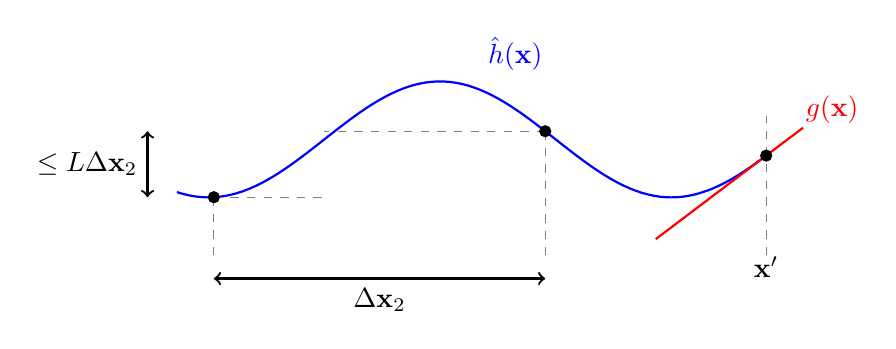
\begin{tikzpicture}[x=0.5cm]
		\begin{axis}[
			hide axis,
			xmin=-3, xmax=6,
			ymin=0, ymax=6,
			domain=0:6,
			samples=100,
			width=10cm,
			height=6cm,
			clip=false
			]
		
			\addplot[blue, thick, domain=-2:6] {2 + sin(deg(x))} 
			node[pos=0.5, above right, yshift=3pt] {$\hat{h}({\bf x})$};
		
		
			\addplot[red, thick, domain=4.5:6.5] 
			{2 + sin(deg(6)) + cos(deg(6))*(x - 6)}
			node[pos=0.95, above right] {$g({\bf x})$};
		
			\addplot[mark=*] coordinates {(6, {2 + sin(deg(6))})};
			    
			\addplot[dashed, gray] coordinates {(6,0) (6,2.4)};
			\node at (axis cs:6, -0.2) {${\bf x}'$};
			    
			    
			\pgfmathsetmacro{\xA}{-1.5}
			\pgfmathsetmacro{\xB}{3}
			\pgfmathsetmacro{\yA}{2 + sin(deg(\xA))}
			\pgfmathsetmacro{\yB}{2 + sin(deg(\xB))}
			\addplot[mark=*, only marks] coordinates {(\xA, \yA) (\xB, \yB)};
		
		
			
			\draw[dashed, gray] (axis cs:\xA,\yA) -- (axis cs:\xA,0);
			\draw[dashed, gray] (axis cs:\xB,\yB) -- (axis cs:\xB,0);
			\draw[dashed, gray] (axis cs:\xA,\yA) -- (axis cs:0,\yA);
			\draw[dashed, gray] (axis cs:\xB,\yB) -- (axis cs:0,\yB);
			 
			\draw[<->, thick] (axis cs:\xA,-0.4) -- node[below] {$\mleft\lVert \Delta {\bf x}\mright\rVert_{2}$} (axis cs:\xB,-0.4);
			
			\draw[<->, thick] (axis cs:-2.4,\yA) -- node[left] {$\leq L \mleft\lVert \Delta {\bf x}\mright\rVert_{2}$} (axis cs:-2.4,\yB);
		\end{axis}
		\vspace*{-10mm}
	\end{tikzpicture}
		\vspace*{-5mm}
	\end{center}
	\caption{
		A trained model $\hat{h}({\bf x})$ that is differentiable at a point ${\bf x}'$ 
		can be locally approximated by a linear map $g \in \mathcal{H}^{(d)}$. This local approximation 
		is determined by the gradient $\nabla \hat{h}({\bf x}')$.}
		\label{fig_linapprox_dict}
	\end{figure}
		See also: model, hypothesis space, linear map, interpretability, LIME.}, 
   first={linear model},
   plural={linear models},
   firstplural={linear models}, 
   text={linear model}
}
	
	
\newglossaryentry{gradstep}
{name={gradient step}, 
	description={Given a differentiable 
		real-valued function $f(\cdot): \mathbb{R}^{d} \rightarrow \mathbb{R}$ 
		and a vector ${\bf w}\in \mathbb{R}^{d}$, the gradient step\index{gradient step} 
		updates ${\bf w}$ by adding the scaled negative gradient $\nabla f({\bf w})$ to obtain 
		the new vector (see Fig. \ref{fig_basic_GD_step_single_dict})
		\begin{equation}
		\label{equ_def_gd_basic_dict} 
		\widehat{{\bf w}}  :={\bf w}- \eta\nabla f({\bf w}).
		\end{equation} 
		Mathematically, the gradient step is an operator $\mathcal{T}^{(f,\eta)}$ 
		that is paramet\-rized by the function $f$ and the step size $\eta$. 
		\begin{figure}[H]
			\begin{center}
				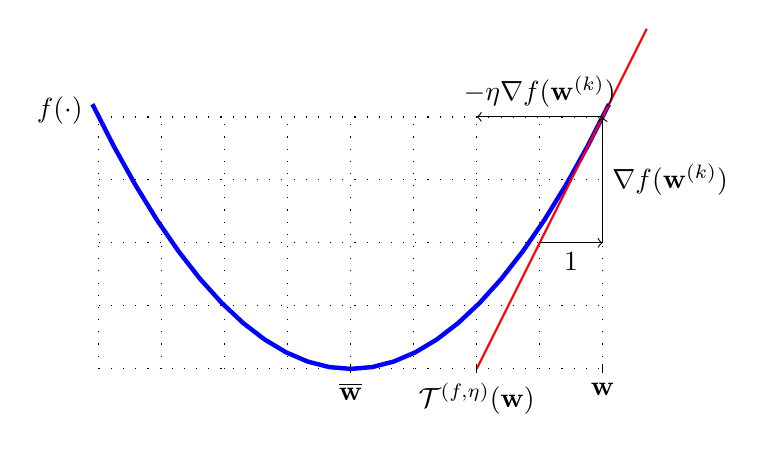
\begin{tikzpicture}[scale=0.8]
					\draw[loosely dotted] (-4,0) grid (4,4);
					\draw[blue, ultra thick, domain=-4.1:4.1] plot (\x,  {(1/4)*\x*\x});
					\draw[red, thick, domain=2:4.7] plot (\x,  {2*\x - 4});
					\draw[<-] (4,4) -- node[right] {$\nabla f({\bf w}^{(k)})$} (4,2);
					\draw[->] (4,4) -- node[above] {$-\eta\nabla f({\bf w}^{(k)})$} (2,4);
					\draw[<-] (4,2) -- node[below] {$1$} (3,2) ;
					
					\node[left] at (-4.1, 4.1) {$f(\cdot)$}; 
					\draw[shift={(0,0)}] (0pt,2pt) -- (0pt,-2pt) node[below] {$\overline{{\bf w}}$};
					\draw[shift={(4,0)}] (0pt,2pt) -- (0pt,-2pt) node[below] {${\bf w}$};
					\draw[shift={(2,0)}] (0pt,2pt) -- (0pt,-2pt) node[below] {$\mathcal{T}^{(f,\eta)}({\bf w})$};
				\end{tikzpicture}
			\end{center}
			\caption{The basic gradient step \eqref{equ_def_gd_basic_dict} maps a given vector ${\bf w}$ 
			to the updated vector ${\bf w}'$. It defines an operator 
			$\mathcal{T}^{(f,\eta)}(\cdot): \mathbb{R}^{d} \rightarrow \mathbb{R}^{d}:
			 {\bf w}\mapsto \widehat{{\bf w}}$.}
			\label{fig_basic_GD_step_single_dict}
		\end{figure}
		Note that the gradient step \eqref{equ_def_gd_basic_dict} optimizes locally—in a neighborhood whose size is 
		determined by the step size $\eta$—a linear approximation 
		to the function $f(\cdot)$. A natural generalization of \eqref{equ_def_gd_basic_dict} is to locally 
		optimize the function itself—instead of its linear approximation—such that
		\begin{align} 
		\label{equ_approx_gd_step_dict}
		\widehat{{\bf w}} = \argmin_{{\bf w}' \in \mathbb{R}^{d}} f({\bf w}')\!+\!\frac{1}{\eta}\mleft\lVert {\bf w}-{\bf w}' \mright\rVert_{2}^2. 
		\end{align}
		We intentionally use the same symbol $\eta$ for the parameter in \eqref{equ_approx_gd_step_dict} 
		as we used for the step size in \eqref{equ_def_gd_basic_dict}. The larger the $\eta$ we choose in 
		\eqref{equ_approx_gd_step_dict}, the more progress the update will make toward reducing the 
		function value $f(\widehat{{\bf w}})$. Note that, much like the gradient step \eqref{equ_def_gd_basic_dict}, 
		the update \eqref{equ_approx_gd_step_dict} also defines an operator 
		that is parameterized by the function $f(\cdot)$ and the learning rate $\eta$. For a convex function  
		$f(\cdot)$, this operator is known as the proximal operator of $f(\cdot)$ \cite{ProximalMethods}. 
					\\ 
		See also: differentiable, function, vector, gradient, step size, neighborhood, generalization, parameter, learning rate, convex, proximal operator.},
	first={gradient step},
	firstplural={gradient steps},
	plural={gradient steps},
	text={gradient step}
}

\newglossaryentry{operator} 
{name={operator}, 
	description={An\index{operator} operator is a function 
	          with domain and co-domain having a specific 
			  mathematical structure such as a vector space, Hilbert space
			  or a metric space \cite{Bauschke:2017,DunfordSchwartz1988}. 
			  Many machine learning (ML) methods involve operators with domain and co-domain 
			  being an Euclidean space.
							\\ 
		See also: vector space, function, Hilbert space.},
	first={operator},
	type=math, 
	plural={operators},
	firstplural={operators},
	text={operator}
}

\newglossaryentry{contractop}
{name={contraction operator},
	description={An\index{contraction operator} operator 
	   $\mathcal{F}: \mathbb{R}^{d} \rightarrow \mathbb{R}^{d}$
		is a contraction if, for some $\kappa\in [0,1)$,
		\begin{equation} 
			\nonumber
			\mleft\lVert  \mathcal{F}{\bf w}\!-\!\mathcal{F}{\bf w}' \mright\rVert_{2}  \leq  \kappa\mleft\lVert {\bf w}\!-\!{\bf w}' \mright\rVert_{2} \mbox{ holds for any } {\bf w},{\bf w}' \in \mathbb{R}^{d}.
		\end{equation}
	},
	first={contraction operator},
	text={contraction operator}, 
	firstplural={contraction operators}, 
	plural={contraction operators}
}
	

\newglossaryentry{proxop}
{name={proximal operator},
	description={Given\index{proximal operator} a convex 
		function $f({\bf w}')$, we define its proximal operator as \cite{Bauschke:2017}, \cite{ProximalMethods}  
		$${\rm\bf prox}_{f(\cdot),\rho}({\bf w}):=\argmin_{{\bf w}' \in \mathbb{R}^{d}} \bigg[ f({\bf w}')\!+\!\frac{\rho}{2} \mleft\lVert {\bf w}- {\bf w}' \mright\rVert_{2}^{2}\bigg] \mbox{ with } \rho > 0. $$ 
		As illustrated in Fig. \ref{fig_proxoperator_opt_dict}, evaluating the proximal operator 
		amounts to minimizing a penalized variant of $f({\bf w}')$. The penalty term is the 
		scaled squared Euclidean distance to a given vector ${\bf w}$ (which is the input to the proximal operator). 
		The proximal operator can be interpreted as a generalization of the gradient step, which is defined 
		for a smooth convex function $f({\bf w}')$. Indeed, taking a 
		gradient step with step size $\eta$ at the current vector ${\bf w}$ 
		is the same as applying the proximal operator of the function $\tilde{f}({\bf w}')= \big( \nabla f({\bf w})\big)\,^{T} ({\bf w}'-{\bf w})$ 
		and using $\rho=1/\eta$.
			\begin{figure}[H]
			\begin{center}
				\begin{tikzpicture}[scale=0.8]
					
					\draw[blue, ultra thick, domain=-4.1:4.1] plot (\x, {(1/4)*\x*\x}) node[above right] {$f({\bf w}')$};		
					
					\draw[red, thick, domain=1:3] plot (\x, {2*(\x - 2)*(\x - 2)}) node[below right] {$\frac{1}{\eta}\mleft\lVert {\bf w}-{\bf w}' \mright\rVert_{2}^{2}$};
					
					
					\draw[shift={(2,0)}] (0pt,2pt) -- (0pt,-2pt) node[below] {${\bf w}$};
					
				\end{tikzpicture}
			\end{center}
			\caption{The proximal operator updates a vector ${\bf w}$ by minimizing a penalized version 
				of the function $f(\cdot)$. The penalty term is the scaled squared Euclidean distance between the optimization 
				variable ${\bf w}'$ and the given vector ${\bf w}$.	\label{fig_proxoperator_opt_dict}}
		\end{figure}
		See also: convex, function, vector, generalization, gradient step, smooth, step size.},
	first={proximal operator},
	text={proximal operator}
}

\newglossaryentry{proximable}
{name={proximable},
	description={A\index{proximable} 
		convex function for which the proximal operator can be computed efficiently is 
		sometimes referred to as proximable or simple \cite{Condat2013}.
					\\ 
		See also: convex, function, proximal operator.},
	first={proximable},
	text={proximable}
}


\newglossaryentry{connected}
{name={connected}, 
	description={An\index{connected} 
	    undirected graph $\mathcal{G}=\left( \mathcal{V},\mathcal{E}\right)$ is 
		connected if for every 
		non-empty subset $\mathcal{V}' \subset \mathcal{V}$ we can find at least one edge 
		connecting a node in $\mathcal{V}'$ with some node in $\mathcal{V}\setminus \mathcal{V}'$.
		\begin{figure}[H]
		\centering
	\begin{tikzpicture}
	
	
	\node[circle, fill=black, inner sep=1.5pt, label=above:{1}] (A1) at (0, 1.5) {};
	\node[above=0.5cm of A1, align=center] {not connected};
	\node[circle, fill=black, inner sep=1.5pt, label=below right:{2}] (B1) [below right=0.8cm and 0.5cm of A1] {};
	\node[circle, fill=black, inner sep=1.5pt, label=below left:{3}] (C1) [below left=0.8cm and 0.5cm of A1] {};
	\draw [line width=1 pt]  (A1) -- (B1);
	
	\begin{scope}[xshift=3.5cm]
		\node[circle, fill=black, inner sep=1.5pt, label=above:{1}] (A2) at (0, 1.5) {};
		\node[above=0.5cm of A2, align=center] {connected};
		\node[circle, fill=black, inner sep=1.5pt, label=below right:{2}] (B2) [below right=0.8cm and 0.5cm of A2] {};
		\node[circle, fill=black, inner sep=1.5pt, label=below left:{3}] (C2) [below left=0.8cm and 0.5cm of A2] {};
		\draw [line width=1 pt]  (A2) -- (B2);
		\draw [line width=1 pt]  (B2) -- (C2);
	\end{scope}
\end{tikzpicture}
\end{figure} 
		See also: undirected graph, algebraic connectivity.}, 
	type=math, 
	first={connected},
	text={connected}
}
	
	
\newglossaryentry{mvndist}
{name={multivariate normal distribution}, 
	description={The\index{multivariate normal distribution} multivariate normal distribution, 
		which is denoted by $\mathcal{N}\left({\bm \mu},{\bf C}\right)$, is a fundamental 
		probabilistic model for numerical feature vectors of fixed dimension $d$. 
		It defines a family of probability distributions over vector-valued random variables (RVs) 
		${\bf x}\in \mathbb{R}^{d}$~\cite{BertsekasProb}, \cite{GrayProbBook}, \cite{Lapidoth09}. 
		Each distribution in this family is fully specified by its mean vector 
		${\bm \mu}\in \mathbb{R}^{d}$ and covariance matrix 
		${\bf C}\in \mathbb{R}^{d\times d}$. When the 
		covariance matrix ${\bf C}$ is invertible, the corresponding probability distribution is 
		characterized by the following probability density function (pdf):
		\[p({\bf x}) = 
 		\frac{1}{\sqrt{(2\pi)^{d} \det\,({\bf C})}} 
 		\exp\left[ -\frac{1}{2} 
 		({\bf x}- {\bm \mu})\,^{T}\, {\bf C}^{-1} 
 		({\bf x}- {\bm \mu}) \right].
 		\]
		Note that this probability density function (pdf) is only defined when ${\bf C}$ is invertible.
   		More generally, any random variable (RV) ${\bf x}\sim \mathcal{N}\left({\bm \mu},{\bf C}\right)$ 
   		admits the following representation:
  		\[
    		{\bf x}= {\bf A}{\bf z}+ {\bm \mu}\]
   		where ${\bf z}\sim \mathcal{N}\left(\mathbf{0},\mathbf{I}\right)$ is a standard normal vector 
   		and ${\bf A}\in \mathbb{R}^{d\times d}$ satisfies ${\bf A}{\bf A}^\top = {\bf C}$. 
   		This representation remains valid even when ${\bf C}$ is singular, in which case ${\bf A}$ 
   		is not full rank~\cite[Ch. 23]{Lapidoth2017}.
   		The family of multivariate normal distributions is exceptional among probabilistic models for numerical 
   		quantities, at least for the following reasons. First, the family is closed under affine 
   		transformations, i.e.,
		\[ 
		{\bf x}\sim \mathcal{N}({\bm \mu},{\bf C}) \mbox{ implies } 
		{\bf B}{\bf x}\!+\!{\bf c}\sim \mathcal{N}\big( {\bf B}{\bm \mu}+{\bf c},{\bf B}{\bf C}{\bf B}\,^{T} \big). 
		\]
		Second, the probability distribution $\mathcal{N}(\mathbf{0},{\bf C})$ maximizes the 
		differential entropy among all distributions with the same covariance matrix ${\bf C}$~\cite{coverthomas}. 
		\\ 
		See also: probabilistic model, probability distribution, standard normal vector, differential entropy, Gaussian random variable (Gaussian RV).}, 
	first={multivariate normal distribution},
	text={multivariate normal distribution}
}

\newglossaryentry{stdnormvec}
{name={standard normal vector}, 
	description={A\index{standard normal vector} standard normal vector is a random 
		vector ${\bf x}=\big(x_{1}, \,\ldots, \,x_{d}\big)\,^{T}$ 
		whose entries are independent and identically distributed (i.i.d.) Gaussian random variables (Gaussian RVs) $x_{j} \sim \mathcal{N}(0,1)$. 
		It is a special case of a multivariate normal distribution, ${\bf x}\sim \mathcal(\mathbf{0},\mathbf{I})$.
		\\ 
		See also: vector, independent and identically distributed (i.i.d.), Gaussian random variable (Gaussian RV), multivariate normal distribution, random variable (RV).}, 
	first={standard normal vector},
	text={standard normal vector}
}

\newglossaryentry{earlystopping}
{name={early stopping}, 
	description={Consider an empirical risk minimization (ERM)-based method that uses an 
	iterative optimization method (such as gradient descent (GD)) to learn model parameters 
	via minimizing the empirical risk on a given training set.
	Early stopping \index{early stopping} refers to terminating the iterations 
	even if they still substantially decrease the empirical risk on the 
	training set. Instead of monitoring the objective function (which is the 
	empirical risk on the training set), early stopping monitors the validation error 
	incurred by the model parameters in each iteration. Early stopping can be 
	interpreted as an implementation of regularization via model 
	pruning. Indeed, terminating an iterative optimization method after a small number 
	of iterations restricts the set of model parameters that can be reached from the 
	initialization (see Fig.\ \ref{fig_early_stopping_dict}).
	\begin{figure}[htbp]
	\centering
		\begin{tikzpicture}[>=Stealth, scale=2]
		
		\fill (0,0) circle (0.6pt) node[above] {\small ${\bf w}^{(0)}$};
		\node at (-0.4,0) {\small $\mathcal{H}^{(1)}$};
		\node at (-1.2,0) {\small $\mathcal{H}^{(2)}$};
			\node at (-2,0) {\small $\mathcal{H}\ldots$};
		
		\draw[densely dotted] (0,0) ellipse (0.8 and 0.4);
		\draw[dashed] (0,0) ellipse (1.6 and 0.8);
		
		\draw[->] (0,0) -- (0.8,0.) node [pos=0.6,above] {\tiny $1$ step};
		\draw[->] (0.0,0.0) -- (0,-0.8) node [pos=0.9,right] {\tiny $2$ steps};
		\end{tikzpicture}
		\caption{A gradient-based method for empirical risk minimization (ERM) using a hypothesis space $\mathcal{H}$ 
		    defines a nested sequence of effective hypothesis spaces 
			$\mathcal{H}^{(1)} \subseteq \mathcal{H}^{(2)} \subseteq \ldots \subseteq \mathcal{H}$. 
			The effective hypothesis space $\mathcal{H}^{(t)}$ is 
		    determined by all model parameters that can be reached from the initialization 
			${\bf w}^{(0)}$ within $t$ gradient steps. \label{fig_early_stopping_dict}}
		\end{figure} \\ 
		See also: gradient-based method, regularization, overfitting.},
	first={early stopping},
	text={early stopping}
}

\newglossaryentry{statasp}
{name={statistical aspects}, 
	description={By statistical aspects\index{statistical aspects} 
		of an machine learning (ML) method, we refer to (properties of) the probability distribution of its output 
		under a probabilistic model for the data fed into the method.
					\\ 
		See also: machine learning (ML), probability distribution, probabilistic model, data.},
	first={statistical aspects},
	text={statistical aspects}
}

\newglossaryentry{compasp}
{name={computational aspects}, 
	description={By computational 
		aspects\index{computational aspects} of an machine learning (ML) method, we mainly refer to the computational 
		resources required for its implementation. For example, if an machine learning (ML) method uses iterative 
		optimization techniques to solve empirical risk minimization (ERM), then its computational aspects include: 1) how 
		many arithmetic operations are needed to implement a single iteration (i.e., a gradient step); 
		and 2) how many iterations are needed to obtain useful model parameters. One important 
		example of an iterative optimization technique is gradient descent (GD).
					\\ 
		See also: machine learning (ML), empirical risk minimization (ERM), gradient step, model parameters, gradient descent (GD).}, 
	first={computational aspects},
	text={computational aspects}
}

\newglossaryentry{zerooneloss}
{name={$\bf 0/1$ loss},
sort={zerooneloss}, 
	description={The $0/1$ loss\index{$0/1$ loss} $L^{(0/1)}\left(\left( {\bf x},y\right),h\right)$ 
		measures the quality of a classifier $h({\bf x})$ that delivers a 
		prediction $\hat{y}$ (e.g., via thresholding \eqref{equ_def_threshold_bin_classifier_dict}) 
		for the label $y$ of a data point with features ${\bf x}$. It is equal to $0$ if 
		the prediction is correct, i.e., 
		$L^{(0/1)}\left(\left( {\bf x},y\right),h\right)=0$ when $\hat{y}=y$. It is 
		equal to $1$ if the prediction is wrong, i.e., $L^{(0/1)}\left(\left( {\bf x},y\right),h\right)=1$ 
		when $\hat{y}\neqy$.
				\\ 
		See also: loss, classifier, prediction, accuracy, label, data point, feature.},
    	first={$0/1$ loss},
	text={$0/1$ loss}
}

\newglossaryentry{probability}
{name={probability}, 
	description={We\index{probability} assign a probability value, typically chosen in the 
		interval $[0,1]$, to each event that can occur in a random experiment  
		\cite{BillingsleyProbMeasure}, \cite{BertsekasProb}, \cite{HalmosMeasure},  \cite{KallenbergBook}.
		\\
		See also: event, random experiment. },
	first={probability},
	firstplural={probabilities},
	plural={probabilities},
	text={probability}
}
	
\newglossaryentry{underfitting}
{name={underfitting},
	description={
		Consider\index{underfitting} an machine learning (ML) method that applies empirical risk minimization (ERM) 
		to learn a hypothesis that minimizes the empirical risk 
		on a given training set. The method is said to underfit if it fails to achieve a sufficiently low empirical risk on the training set. 
		Underfitting typically occurs when the chosen model is too simple 
		to capture the underlying relationship between features and 
		labels. 
			\begin{figure}[H]
		\begin{center}
			\begin{tikzpicture}[scale=1.0]
				
				\def\slope{0.35}
				\def\intercept{2.0}
				\draw[thick,dashed,domain=0:6.5,variable=\x]
				plot({\x},{\slope*\x+\intercept});
				\node[above right] at (6.5,{\slope*6.5+\intercept}) {$h(x)$};
				
				
				\foreach \i/\x/\y in {1/0.6/2.4, 2/1.2/2.1, 3/1.8/2.0, 4/2.4/2.3,
					5/3.0/3.1, 6/3.6/4.0, 7/4.2/5.2, 8/4.8/6.0,
					9/5.4/6.3, 10/6.0/6.1} {
					\node[circle,draw,fill=blue!60,minimum size=5pt,inner sep=0pt] (p\i) at (\x,\y) {};
					
					\draw[<->,color=blue!70] (\x,{\slope*\x+\intercept}) -- (p\i);
				}
			\end{tikzpicture}
			\caption{No linear hypothesis $h$ can capture the relation 
			         between features and labels for 
					 the depicted training set. Thus, any method that uses a 
					 linear model will underfit this training set.}
			\label{fig_underfitting_min_dict}
		\end{center}
	\end{figure} 
		For example, a machine learning (ML) method using a linear model 
		on data with a highly non-linear relation between features 
		and label will not be able to learn a hypothesis with small 
		average loss on the training set, let alone a small risk. 
					\\ 
		See also: model, training set, risk, overfitting.},
	first={underfitting},
	text={underfitting}
}

\newglossaryentry{overfitting}
{name={overfitting},
	description={Consider\index{overfitting} an 
		machine learning (ML) method that uses empirical risk minimization (ERM) to learn a hypothesis with the 
		minimum empirical risk on a given training set. Such a method is 
		overfitting the training set if it learns a hypothesis with a  
		empirical risk on the training set that a significantly smaller than the 
		average loss outside the training set. In other words, if a machine learning (ML) 
		method overfits it has a large generalization gap. 
					\\ 
		See also: empirical risk minimization (ERM), generalization, validation, generalization gap.},
	first={overfitting},
	text={overfitting}
}

\newglossaryentry{gdpr}
{name={general data protection regulation (GDPR)},
	description={The\index{general data protection regulation (GDPR)} GDPR
			was enacted by the European Union (EU), effective from 25 May 2018 \cite{GDPR2016}. 
			It safeguards the privacy and data rights of individuals in the EU. 
			The GDPR has significant implications for how data are collected, stored, 
			and used in machine learning (ML) applications. Key provisions include the following:
			\begin{itemize}
				\item Data minimization principle: machine learning (ML) systems should only use the necessary 
				amount of personal 
				data for their purpose.
				\item Transparency and explainability: machine learning (ML) systems should 
				enable their users to 
				understand how the systems make decisions that impact the users.
				\item Data subject rights: Users should get an opportunity to access, 
				rectify, and delete their personal data, as well as to object to automated 
				decision-making and profiling.
				\item Accountability: Organizations must ensure robust data security 
				and demonstrate compliance through documentation and regular audits.
			\end{itemize}
		See also: data, machine learning (ML), data minimization principle, transparency, explainability.}, 
	first={general data protection regulation (GDPR)},
	text={GDPR}
}

\newglossaryentry{normaldist} 
{name={normal distribution}, 
 description={See\index{normal distribution} Gaussian random variable (Gaussian RV).},
 first={normal distribution}, 
 firstplural={normal distributions},
 plural={normal distributions},
 type=math, 
 text={normal distribution}
}
	
\newglossaryentry{gaussrv}
{name={Gaussian random variable (Gaussian RV)}, 
	description={A \index{Gaussian random variable (Gaussian RV)} standard Gaussian random variable (RV) is a 
		real-valued random variable (RV) $x$ with probability density function (pdf) \cite{BertsekasProb}, \cite{GrayProbBook}, \cite{papoulis}
		\begin{equation}
			\nonumber
			p(x) = \frac{1}{\sqrt{2\pi}} \exp\,(-x^2/2). 
		\end{equation}
		Given a standard Gaussian random variable (RV) $x$, we can construct a general Gaussian 
		random variable (RV) $x'$ with mean $\mu$ and variance $\sigma^2$ via $x' :=\sigma x + \mu$. 
		The probability distribution of a Gaussian random variable (RV) is referred to as normal distribution, 
		denoted by $\mathcal{N}\left(\mu,\sigma^{2}\right)$. 
		\\ 
		A Gaussian random vector ${\bf x}\in \mathbb{R}^{d}$ with 
		covariance matrix $\mathbf{C}$ and mean ${\bm \mu}$ can be constructed as \cite{GrayProbBook}, \cite{papoulis}, \cite{Lapidoth09}
		\[
		{\bf x}:=\mathbf{A} {\bf z}+ {\bm \mu}
		\]
		where ${\bf z}:=\big( z_{1}, \,\ldots, \,z_{d} \big)\,^{T}$ is a vector 
		of independent and identically distributed (i.i.d.) standard Gaussian random variables (RVs), and ${\bf A}\in \mathbb{R}^{d\times d}$ is any matrix satisfying ${\bf A}{\bf A}\,^{T} = {\bf C}$. 
		The probability distribution of a Gaussian random vector is referred to as the multivariate normal distribution, 
		denoted by $\mathcal{N}\left(\bm \mu,\mathbf{C}\right)$.
		\\
		We can interpret a Gaussian random vector ${\bf x}=\big(\feature_{1},\,\ldots,\,\feature_{d}\big)$ as a stochastic process 
		indexed by the set $\mathcal{I}=\{1,\,\ldots,\,d\}$. A GPs is a 
		stochastic process over an arbitray index set $\mathcal{I}$ such that any restriction 
		to a finite subset $\mathcal{I}' \subseteq \mathcal{I}$ yields a Gaussian 
		random vector \cite{Rasmussen2006Gaussian}.
  		\\
        		Gaussian random variables (RVs) are widely used probabilistic models in the 
				statistical analysis of machine learning (ML) methods. Their significance arises 
				partly from the central limit theorem (CLT) which provides conditions under which 
				the average of many independent random variables (RVs) (not necessarily Gaussian themselves) 
				tends toward a Gaussian random variable (RV) \cite{ross2013first}.
		\\ 
		The multivariate normal distribution is also distinct in that it represents maximum uncertainty. 
		Among all vector-valued random variables (RVs) with a given covariance matrix ${\bf C}$, the 
		random variable (RV) ${\bf x}\sim \mathcal{N}\left(\bm \mu,\mathbf{C}\right)$ maximizes differential entropy 
		\cite[Th. 8.6.5]{coverthomas}. This makes GPs a natural choice for 
		capturing uncertainty or the lack of (domain) knowledge.
		\\ 
		See also: multivariate normal distribution, GP, probabilistic model, central limit theorem (CLT), differential entropy.},
	first={Gaussian random variable (Gaussian RV)},
	type=math, 
	plural={Gaussian RVs}, 
	firstplural={Gaussian random variables (Gaussian RVs)}, 
	text={Gaussian RV}
}

\newglossaryentry{gaussian} 
{name={Gaussian}, 
 description={See\index{Gaussian} Gaussian random variable (Gaussian RV).},
 first={Gaussian},
 type=math,
 text={Gaussian},
 firstplural={Gaussians},  
 plural={Gaussians}
 }
	
\newglossaryentry{clt}
{name={central limit theorem (CLT)},
	description={Consider a sequence of independent and identically distributed (i.i.d.) random variables (RVs) \( x^{(r)} \), for \( r= 1, \,2, \,\ldots \), 
		each with mean zero and finite variance \( \sigma^2 > 0 \). 
		The \index{central limit theorem (CLT)} CLT states that the normalized sum 
		\[
		s^{(m)} :=\frac{1}{\sqrt{m}} \sum_{r= 1}^{m} x^{(r)} 
		\]
		converges in distribution to a Gaussian random variable (Gaussian RV) with mean zero and variance \( \sigma^2 \) as \( m\to \infty \) \cite[Proposition~2.17]{AsympVanderVaartBook}.
		One elegant way to derive the CLT is via the characteristic function of the normalized sum \( s^{(m)} \). 
		Let $ \phi(t) = \mathbb{E} \big\{ \exp \big( j t x\big) \big\}$ (with the imaginary unit $j = \sqrt{-1}$) 
		be the common characteristic function of each sum and $x^{(r)}$, and let \( \phi^{(m)}(t) \) 
		denote the characteristic function of \( s^{(m)} \). Define an operator \( \mathcal{T} \) acting on characteristic functions 
		such that
		\[
		\phi^{(m)}(t) = \mathcal{T}(\phi^{(m-1)})(t) :=\phi\left( \frac{t}{\sqrt{m}} \right) \cdot \phi^{(m-1)}\left( \frac{\sqrt{m-1}}{\sqrt{m}} t \right).
		\]
		This fixed-point iteration captures the effect of recursively adding an independent and identically distributed (i.i.d.) random variable (RV) ${\bf x}^{(m)}$ 
		and rescaling. Iteratively applying \( \mathcal{T} \) leads to convergence of \( \phi^{(m)}(t) \) toward the fixed point
		\[
		\phi^*(t) = \exp\,(-t^2 \sigma^2 / 2)
		\]
		which is the characteristic function of a Gaussian random variable (Gaussian RV) with mean zero and variance 
		\( \sigma^2 \). Generalizations of the CLT allow for dependent or nonidentically distributed random variables (RVs) \cite[Sec.~2.8]{AsympVanderVaartBook}.
		\begin{figure}[H]
			\centering
			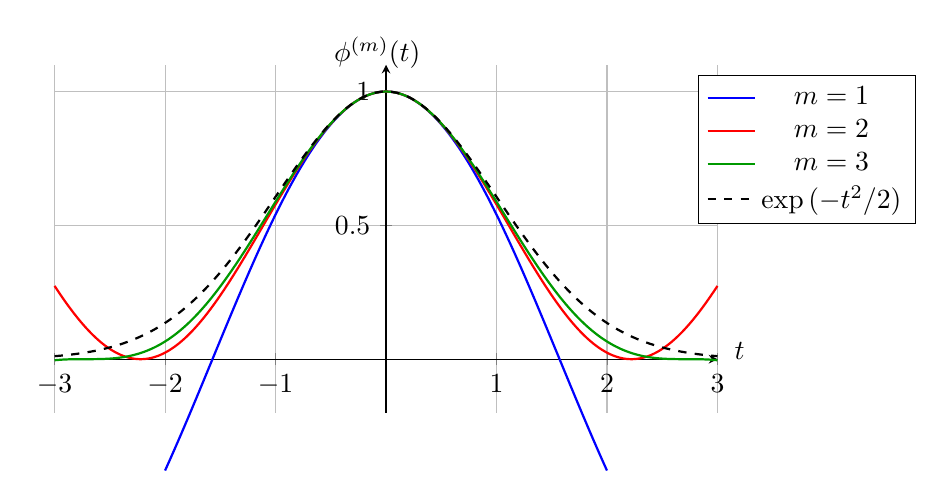
\begin{tikzpicture}
			\begin{axis}[
			width=10cm,
			height=6cm,
			xlabel={},
			ylabel={},
			legend style={at={(0.97,0.97)}, anchor=north west},
			domain=-3:3,
			ylabel style={
			yshift=10pt   
			},
			samples=400,
			ymin=-0.2, ymax=1.1,
			axis lines=middle,
			clip=false,
			grid=both,
			]
			\addplot[thick, blue,domain=-2:2] {cos(x/sqrt(1) r)^1};
			\addlegendentry{$m=1$}
			\addplot[thick, red] {cos(x/sqrt(2) r)^2};
			\addlegendentry{$m=2$}
			\addplot[thick, green!60!black] {cos(x/sqrt(3) r)^3};
			\addlegendentry{$m=3$}
			\addplot[thick, dashed, black] {exp(-x^2/2)};
			\addlegendentry{$\exp\,(-t^2/2)$}
			\node[anchor=south, rotate=0] at (axis cs:-0.08,1.05) {$\phi^{(m)}(t)$};
			\node[anchor=north, rotate=0] at (axis cs: 3.2,0.1) {$t$};
			\end{axis}
			\end{tikzpicture}
			\caption{Characteristic functions of normalized sums of independent and identically distributed (i.i.d.) random variables (RVs) $x^{(r)} \in \{-1,1\}$ 
			for $r=1,\,\ldots,\,m$ compared to the Gaussian limit.}
		\end{figure}
		See also: random variable (RV), Gaussian random variable (Gaussian RV).},
	first={central limit theorem (CLT)},
	type=math, 
	text={CLT}
}


\newglossaryentry{GaussProc}
{name={Gaussian process (GP)},
  description={A \index{Gaussian process (GP)}GP is a collection of random variables (RVs) 
  	$\{f({\bf x})\}_{{\bf x}\in \mathcal{X}}$ indexed by input values ${\bf x}$ 
  	from some input space $\mathcal{X}$ such that, for any finite subset 
  	${\bf x}^{(1)}, \,\ldots, \,{\bf x}^{(m)} \in \mathcal{X}$, 
  	the corresponding random variables (RVs) $f({\bf x}^{(1)}, \,\ldots, \,{\bf x}^{(m)})$ 
	have a joint multivariate normal distribution 
  	\[
  	f \left( {\bf x}^{(1)}, \,\ldots, \,{\bf x}^{(m)} \right) \sim \mathcal{N}(\boldsymbol{\mu}, \mathbf{K}).
  	\]
  	For a fixed input space $\mathcal{X}$, a GP is 
	fully specified (or parameterized) by: 1) a mean function 
	$\mu({\bf x}) = \mathbb{E} \{ f({\bf x})\}$; and 2) 
	a covariance function $K\big({\bf x},{\bf x}'\big)= \mathbb{E} \{ \big(f({\bf x})-\mu({\bf x})\big) \big(f({\bf x}')-\mu({\bf x}')\big) \big\}$.\\
  	{\bf Example.} We can interpret the temperature distribution across Finland (at a specific 
  	point in time) as the realization of a GP $f({\bf x})$, where each input 
	${\bf x}= (\text{lat}, \text{lon})$ denotes a geographic location. Temperature 
	observations from Finnish Meteorological Institute (FMI) weather stations provide values $f({\bf x})$ at specific 
	locations (see Fig. \ref{fig_gp_FMI_dict}). A GP allows us to predict the temperature 
	nearby Finnish Meteorological Institute (FMI) weather stations and to quantify the uncertainty 
  	of these predictions. 
  	\begin{figure}[H]
  	\begin{center}
  		\begin{tikzpicture}
		\begin{axis}[
		axis equal,
		hide axis,
		scale=1.2,
		xmin=17, xmax=32,
		ymin=55, ymax=71,
		
		
		clip=true
		]
		
		\addplot[
		color=black,
		thick
		] table [x=lon, y=lat, col sep=comma] {assets/finland_border.csv};
		
		\addplot[
		only marks,
		mark=*,
		mark options={fill=blue},
		color=black
		] table [x=lon, y=lat, col sep=comma] {assets/fmi_stations_subset.csv};
		
		\draw[->, thick] (axis cs:19,59) -- (axis cs:25.5,59) node[anchor=west] {longitude (lon)};
		\draw[->, thick] (axis cs:19,59) -- (axis cs:19,65.5) node[anchor=south] {latitude (lat)};
		\end{axis}
		\end{tikzpicture}
		\vspace*{-15mm}
	\end{center}
	\caption{For a given point in time, we can interpret the current temperature distribution 
	over Finland as a realization of a GP indexed by geographic coordinates and 
	sampled at Finnish Meteorological Institute (FMI) weather stations. The weather stations are indicated by blue dots. \label{fig_gp_FMI_dict}}
	\end{figure}
	See also: multivariate normal distribution, uncertainty, Gaussian random variable (Gaussian RV).}, 
  first={GP}, 
  type=math, 
  text={GP}
}

\newglossaryentry{trustAI}
{name={trustworthy artificial intelligence (trustworthy AI)},
	description={Besides the computational aspects and statistical aspects, a third main design aspect of 
		machine learning (ML) methods is their trustworthiness\index{trustworthy artificial intelligence (trustworthy AI)} \cite{pfau2024engineeringtrustworthyaideveloper}. 
		The EU has put forward seven key requirements (KRs) for trustworthy 
		AI (which typically build on machine learning (ML) methods) \cite{ALTAIEU}: 
	\begin{enumerate}[label=\arabic*)]
		\item KR1 – Human agency and oversight;
		\item KR2 – Technical robustness and safety;
		\item KR3 – Privacy and data governance;
		\item KR4 – Transparency;
		\item KR5 – Diversity, non-discrimination and fairness; 
		\item KR6 – Societal and environmental well-being;
		\item KR7 – Accountability. 
	\end{enumerate}
		See also: computational aspects, statistical aspects, machine learning (ML), AI, robustness, data, transparency.},
	first={trustworthy artificial intelligence (trustworthy AI)},
	text={trustworthy AI}
}

\newglossaryentry{sqerrloss}
{name={squared error loss},
	description={The squared 
		error\index{squared error loss} loss measures the prediction error of a 
		hypothesis $h$ when predicting a numeric label $y\in \mathbb{R}$ 
		from the features ${\bf x}$ of a data point. It is defined as 
		\begin{equation} 
			\nonumber
			L\left(({\bf x},y),h\right) :=\big(y- \underbrace{h({\bf x})}_{=\hat{y}} \big)^{2}. 
		\end{equation} 
			\\ 
		See also: loss, prediction, hypothesis, label, feature, data point.},
	first={squared error loss},
	text={squared error loss}
}


 \newglossaryentry{projection}
 {name={projection}, 
       description={Consider\index{projection} a subset $\mathcal{W}\subseteq \mathbb{R}^{d}$ of 
	   the $d$-dimensional Euclidean space. We define the projection $P_{\mathcal{W}}\big( {\bf w}\big) $
	   of a vector ${\bf w}\in \mathbb{R}^{d}$ onto $\mathcal{W}$ as
	   \begin{equation} 
   	   	\nonumber
		\label{equ_def_proj_generic_dict}
  	    	P_{\mathcal{W}}\big( {\bf w}\big)  = \argmin_{{\bf w}' \in \mathcal{W}} \mleft\lVert {\bf w}- {\bf w}' \mright\rVert_{2}. 
        	    \end{equation}
	    In other words, $P_{\mathcal{W}}\big( {\bf w}\big) $ is the vector in $\mathcal{W}$ 
	    that is closest to ${\bf w}$. The projection is only well defined for subsets $\mathcal{W}$ 
	    for which the above minimum exists \cite{BoydConvexBook}.
		 			\\ 
	    See also: Euclidean space, vector, minimum.},
	first={projection},
	text={projection}
}


\newglossaryentry{projgd}
{name={projected gradient descent (projected GD)},
	description={Consider an empirical risk minimization (ERM)-based method that uses a parameterized model with  
		parameter space $\mathcal{W}\subseteq \mathbb{R}^{d}$. Even if 
		the objective function of empirical risk minimization (ERM) is smooth, we cannot use basic gradient descent (GD), as 
		it does not take into account constraints on the optimization variable (i.e., the model parameters). 
		Projected\index{projected gradient descent (projected GD)} gradient descent (GD) 
		extends basic gradient descent (GD) to address this issue. 
		A single iteration of projected gradient descent (GD) consists of first taking a gradient step 
		and then projecting the result back onto the parameter space. 
		See Fig. \ref{fig_projected_GD_dict} for a visual illustration.
		\begin{figure}[H]
		\begin{center}
			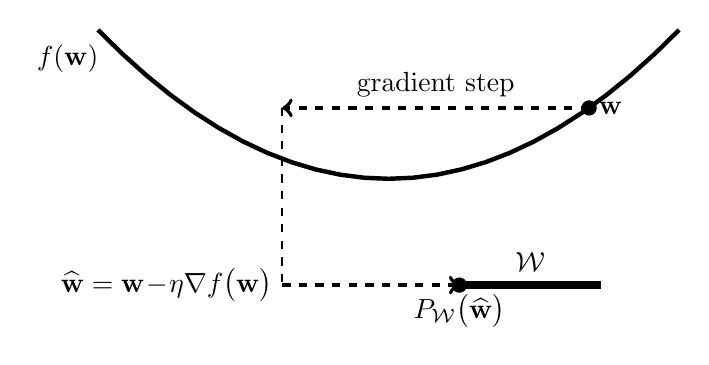
\begin{tikzpicture}[scale=0.9]
			\node [right] at (-5.1,1.7) {$f({\bf w})$} ;
			\draw[ultra thick, domain=-4.1:4.1] plot (\x,  {(1/8)*\x*\x});
		
			\draw [fill] (2.83,1) circle [radius=0.1] node[right] {${\bf w}$};
			\draw[line width =0.5mm,dashed,->] (2.83,1) -- node[midway,above] {gradient step} (-1.5,1);
			\draw[line width =0.2mm,dashed] (-1.5,1) --(-1.5,-1.5)  node [below, left]{$\widehat{{\bf w}}={\bf w}\!-\!\eta\nabla f\big({\bf w}\big)$} ;
			\draw[line width =0.5mm,dashed,->] (-1.5,-1.5)  -- node[midway,above] {} (1,-1.5) ; 
			\draw [fill] (1,-1.5) circle [radius=0.1] node[below] {$P_{\mathcal{W}}\big( \widehat{{\bf w}}\big) $};
			\draw[line width=1mm] (1,-1.5) -- (3,-1.5) node[midway, above] {$\mathcal{W}$};
			\end{tikzpicture}
		\vspace*{-5mm}
		\end{center}
		\caption{Projected gradient descent (GD) augments a basic gradient step with a projection back 
		onto the constraint set $\mathcal{W}$.}
		\label{fig_projected_GD_dict}
		\end{figure}
		See also: empirical risk minimization (ERM), model, parameter space, objective function, smooth, gradient descent (GD), model parameters, gradient step, projection.},
	first={projected gradient descent (projected GD)},
	type=math, 
	text={projected GD}
}

\newglossaryentry{diffpriv}
{name={differential privacy (DP)},
  description={Consider\index{differential privacy (DP)} some machine learning (ML) method $\mathcal{A}$ 
  	that reads in a dataset (e.g., the training set 
  	used for empirical risk minimization (ERM)) and delivers some output $\mathcal{A}(\mathcal{D})$. The output 
  	could be either the learned model parameters or the predictions for specific data points. 
  	DP is a precise measure of privacy leakage incurred by revealing the 
  	output. Roughly speaking, an machine learning (ML) method is differentially private if the probability distribution 
  	of the output $\mathcal{A}(\mathcal{D})$ remains largely unchanged if the sensitive attribute 
  	of one data point in the training set is changed. Note that DP 
  	builds on a probabilistic model for an machine learning (ML) method, i.e., we interpret its output $\mathcal{A}(\mathcal{D})$ 
  	as the realization of a random variable (RV). The randomness in the output can be ensured 
  	by intentionally adding the realization of an auxiliary random variable (RV) (i.e., adding noise) to 
  	the output of the machine learning (ML) method.
				\\ 
	See also: privacy leakage, sensitive attribute, privacy attack, privacy funnel.}, 
  first={DP}, 
  text={DP} 
}

\newglossaryentry{robustness}
{name={robustness},
	description={Robustness\index{robustness} is a key requirement for trustworthy artificial intelligence (trustworthy AI). It
		refers to the property of an machine learning (ML) system to maintain acceptable performance even when 
		subjected to different forms of perturbations. These perturbations may affect the features 
		of a data point in order to manipulate the prediction delivered by a trained machine learning (ML) model. 
		Robustness also includes the stability of empirical risk minimization (ERM)-based methods against perturbations 
		of the training set. Such perturbations can occur within data poisoning attacks. 
		\\ 
		See also: trustworthy artificial intelligence (trustworthy AI),stability,data poisoning, attack.}, 
	first={robustness}, 
	text={robustness} 
}


\newglossaryentry{stability}
{name={stability},
	description={
	Mathematically, a machine learning (ML) method is a map $\mathcal{A}$ from a given dataset $\mathcal{D}$ 
	to an output $\mathcal{A}(\mathcal{D})$. As a case in point, consider an empirical risk minimization (ERM)-based 
	machine learning (ML) method that maps a training set $\mathcal{D}$ to the learned model parameters 
	$\mathcal{A}(\mathcal{D}) = \widehat{{\bf w}}$ which achieve the minimum average loss 
	on the training set. Instead of the learned model parameters, the 
	output $\mathcal{A}(\mathcal{D})$ could also be the predictions obtained from 
	the trained model. Stability\index{stability} refers to the desirable property 
	of $\mathcal{A}$ that small changes in the input dataset $\mathcal{D}$ result in small 
	changes in the output $\mathcal{A}(\mathcal{D})$. The notion of stability is intimately related 
	to the notion of generalization. In particular, there are formal notions of stability  
	that allow to bound the generalization gap (see \cite[Ch.~13]{ShalevMLBook}).
		To build intuition, consider the three datasets depicted in Fig. \ref{fig_three_data_stability_dict}, each 
		of which is equally likely under the same data-generating probability distribution. Since the 
		optimal model parameters are determined by this underlying probability distribution, an accurate 
		machine learning (ML) method $\mathcal{A}$ should return the same (or very similar) output $\mathcal{A}(\mathcal{D})$ 
		for all three datasets. In other words, any useful $\mathcal{A}$ must be robust to 
		variability in sample realizations from the same probability distribution, i.e., it must be stable. 
		\begin{figure}[H]
			\centering
			\begin{tikzpicture}
				\begin{axis}[
				
				    axis lines=none,
					xlabel={$r$},
					ylabel={},
					legend pos=north west,
					ymin=0, ymax=10,
					xtick={1,2,3,4,5},
				
					grid style=dashed,
					every axis plot/.append style={very thick}
					]
					
					\addplot+[only marks,mark=*] coordinates {
						(1,2) (2,4) (3,3) (4,5) (5,7)
					};
				
					
					\addplot+[only marks,mark=square*] coordinates {
						(1,3) (2,2) (3,6) (4,4) (5,5)
					};
				
					
					\addplot+[only marks,mark=triangle*] coordinates {
						(1,5) (2,7) (3,4) (4,6) (5,3)
					};
				
				\end{axis}
			\end{tikzpicture}
			\caption{Three datasets $\mathcal{D}^{(*)}$, $\mathcal{D}^{(\square)}$, 
			and $\mathcal{D}^{(\triangle)}$, each sampled independently from the same 
			data-generating probability distribution. A stable machine learning (ML) method should return 
			similar outputs when trained on any of these datasets. \label{fig_three_data_stability_dict}}
		\end{figure}
		See also: generalization, robustness.}, 
	first={stability}, 
	text={stability} 
}

\newglossaryentry{privprot}
{name={privacy protection},
     description={Consider\index{privacy protection} some machine learning (ML) method $\mathcal{A}$ that reads 
	 	in a dataset $\mathcal{D}$ and delivers some output $\mathcal{A}(\mathcal{D})$. The output 
	 	could be the learned model parameters $\widehat{{\bf w}}$ or the prediction 
	 	$\hat{h}({\bf x})$ obtained for a specific data point with features 
	 	${\bf x}$. Many important machine learning (ML) applications involve data points 
		representing humans. Each data point is characterized by features ${\bf x}$, 
		potentially a label $y$, and a sensitive attribute $s$ (e.g., a recent medical diagnosis). 
		Roughly speaking, privacy protection means that it should be impossible to infer, from the output $\mathcal{A}(\mathcal{D})$, 
		any of the sensitive attributes of data points in $\mathcal{D}$. Mathematically, privacy protection requires non-invertibility 
		of the map $\mathcal{A}(\mathcal{D})$. In general, just making $\mathcal{A}(\mathcal{D})$ non-invertible 
		is typically insufficient for privacy protection. We need to make $\mathcal{A}(\mathcal{D})$ sufficiently non-invertible. 
					\\ 
		See also: machine learning (ML), dataset, model parameters, prediction, data point, feature, label, sensitive attribute, map.}, 
	first={privacy protection}, 
	text={privacy protection} 
}

\newglossaryentry{privleakage}
{name={privacy leakage},
	description={Consider\index{privacy leakage} an machine learning (ML) application that processes a 
		dataset $\mathcal{D}$ and delivers some output, such as the predictions 
		obtained for new data points. Privacy leakage arises 
		if the output carries information about a private (or sensitive) feature of 
		a data point of $\mathcal{D}$ (such as a human). Based on a probabilistic model 
		for the data generation, we can measure the privacy leakage via the MI 
		between the output and the sensitive feature. Another quantitative measure of privacy leakage 
		is DP. The relations between different measures of privacy leakage have been 
		studied in the literature (see \cite{InfThDiffPriv}). 
				\\ 
		See also: MI, DP, privacy attack, general data protection regulation (GDPR). }, 
	first={privacy leakage}, 
	text={privacy leakage} 
}


\newglossaryentry{probmodel}
{name={probabilistic model}, plural={probabilistic models},
	description={A probabilistic model\index{probabilistic model} interprets the 
	             generation of data points as random variables (RVs) with a joint probability distribution. 
				This joint probability distribution typically involves parameters that have to 
				be manually chosen or learned via statistical inference methods such as 
				maximum likelihood estimation \cite{LC}.
					\\ 
		See also: model, data point, realization, random variable (RV), probability distribution, parameter, maximum likelihood. }, 
	first={probabilistic model}, 
	type=math,
	text={probabilistic model} 
}


\newglossaryentry{mean}
{name={mean}, plural={means},
	description={The \index{mean} mean of a random variable (RV) ${\bf x}$, which takes 
 		on values in a Euclidean space $\mathbb{R}^{d}$, is its 
 		expectation $\mathbb{E} \{{\bf x}\}$. It is defined as the Lebesgue 
 		integral of ${\bf x}$ with respect to the underlying probability distribution $P$ (e.g., 
		see \cite{RudinBookPrinciplesMatheAnalysis} or \cite{BillingsleyProbMeasure}), i.e.,
		\[
			\mathbb{E} \{{\bf x}\} = \int_{\mathbb{R}^{d}} {\bf x}\, \mathrm{d}P({\bf x}).
		\]  
		We also use the term to refer to the average of a finite dataset
		$\mathcal{D}= \left\{ {\bf x}^{(1)}, \,\ldots, \,{\bf x}^{(m)} \in \mathbb{R}^{d}\right\}$. 
		However, these two definitions are essentially the same. Indeed, we can use 
		a dataset to construct a discrete random variable (RV) $\widetilde{{\bf x}}^{(\mathcal{D})}={\bf x}^{(I)}$ on 
		the sample space $\{1, \,\ldots, \,m\}$. Here, the index $I$ is 
		chosen uniformly at random, $\mathbb{P}\left(I=r\right)=1/m$ for all 
		$r=1,\ldots,m$. The mean of $\widetilde{{\bf x}}^{(\mathcal{D})}$ is 
		precisely the average $({1}/{m}) \sum_{r=1}^{m} {\bf x}^{(r)}$.
		For a random variable (RV) with finite second-order moment, i.e., 
		$\mathbb{E} \{ \mleft\lVert {\bf x}\mright\rVert_{2}^{2} \}$ is well-defined and fnite, 
		the mean is characterized as the solution of the 
		following risk minimization problem \cite{BertsekasProb}:
		\[
			\mathbb{E} \{{\bf x}\} = \argmin_{{\bf c}\in \mathbb{R}^{d}} 
			\mathbb{E} \big\{\mleft\lVert {\bf x}- {\bf c}\mright\rVert_{2}^{2}\big \}.
		\]
		For the random variable (RV) $\widetilde{{\bf x}}^{(\mathcal{D})}$, associated with a dataset, 
		this optimization problem reduces to empirical risk minimization (ERM) with squared error loss on $\mathcal{D}$. 
		\\ 
		See also: random variable (RV), expectation, probability distribution, empirical risk minimization (ERM).}, 
	first={mean}, 
	type=math,
	text={mean} 
}

\newglossaryentry{median}
{name={median}, 
plural={medians},
	description={A\index{median} median $\mathrm{med}\,(x)$ of a real-valued random variable (RV) $x$ 
 		is any number $M \in \mathbb{R}$ such that $\mathbb{P}\left( x \leq M\right) \geq 1/2$ and 
		$\mathbb{P}\left( x \geq M\right) \geq 1/2$ 
		(see Fig. \ref{fig_median1_dict}) \cite{LC}. 
 		\begin{figure}[H]
			\begin{center}
			\begin{tikzpicture}
 			\begin{axis}[
    			axis lines=middle,
    			xlabel={},
    			ylabel={},
    			ymin=0, ymax=1.1,
    			xmin=-2, xmax=6,
    			xtick=\empty,
    			ytick={0,1/2,1},
    			domain=-2:6,
    			samples=200,
    			width=10cm,
    			height=6cm,
    			smooth,
    			enlargelimits=true,
    			clip=false
  			]
    			
			\addplot[thick, blue, name path=cdf] {1/(1 + exp(-(x - 1)))} node[pos=0.5, above, yshift=15pt] {$\mathbb{P}\left(x \leq \eta\right)$};    
    			\draw[dashed, gray] (axis cs:1,0) -- (axis cs:1,0.5); 
    			\draw[dashed, gray] (axis cs:-2,0.5) -- (axis cs:1,0.5); 
    			
   			\filldraw[red] (axis cs:1,0.5) circle (2pt);
  		    \node[below] at (axis cs:1,0) {$M$};
			\node[above right] at (axis cs:6.3,0) {$\eta$};
    			
  			\end{axis}
			\end{tikzpicture} 
			\end{center}
			\caption{The median of a real-valued random variable (RV) is any number $M$ 
			that partitions $\mathbb{R}$ into two rays with equal probability. \label{fig_median1_dict}}
 		\end{figure}  
 		We can define the median $\mathrm{med}\,(\mathcal{D})$ 
 		of a dataset $\mathcal{D}= \{ x^{(1)}, \,\ldots, \,x^{(m)} \in \mathbb{R} \}$ 
 		via a specific random variable (RV) $\tilde{x}^{(\mathcal{D})}$ that is naturally associated with $\mathcal{D}$. 
 		In particular, this random variable (RV) is defined on the sample space $\{1, \,\ldots, \,m\}$ 
		via $\tilde{x}^{(\mathcal{D})} :=x^{(I)}$. Here, the index $I$ is chosen uniformly 
		at random, i.e., $\mathbb{P}\left(I = r\right)=1/m$ for 
 		all $r=1, \,\ldots, \,m$. If the random variable (RV) $x$ is integrable, any 
		median of $x$ solves the optimization problem: 
 		$$\min_{x' \in \mathbb{R}} \mathbb{E} {|x - x'|}.$$ 
		For a the above random variable (RV) $\tilde{x}$ (constructed from a dataset $\mathcal{D}$), 
		this optimization problem is empirical risk minimization (ERM) on $\mathcal{D}$ using absolute error loss. 
 		Like the mean, the median of a dataset $\mathcal{D}$ can also be used 
 		to estimate parameters of an underlying probabilistic model. Compared 
 		with the mean, the median is more robust to outliers. For example, 
 		a median of a dataset $\mathcal{D}$ with more than one data point does not 
 		change even if we arbitrarily increase the largest element of $\mathcal{D}$ (see Fig. \ref{fig_median2_dict}). 
		In contrast, the mean will increase arbitrarily.
		\begin{figure}[H]
		\centering
		\begin{tikzpicture}[scale=0.7, y=0.5cm, x=0.5cm]
			\begin{scope}
				\foreach \x/\y in {
					1/2, 4/3, 7/4
				} {
					\draw[dashed, gray] (\x, 0) -- (\x, \y);
					\filldraw[blue] (\x, \y) circle (2pt);
					\node[circle, inner sep=0pt] (ptA\x) at (\x, \y) {};
				}
				\draw[dashed, thick] (0.5, 3) -- (10.5, 3) node[right] {$\mathrm{med}\,(\mathcal{D})\!=\!{\rm mean}(\mathcal{D})$};
				\node at (7.5, -4) {(a)};
			\end{scope}
			\begin{scope}[xshift=12cm]
				\foreach \x/\y in {
					1/2, 4/3, 7/10
				} {
					\draw[dashed, gray] (\x, 0) -- (\x, \y);
					\filldraw[blue] (\x, \y) circle (2pt);
					\node[circle, inner sep=0pt] (ptB\x) at (\x, \y) {};
				}
				\draw[dashed, thick] (0.5, 7.5) -- (10.5, 7.5) node[right] 
				{${\rm mean}\,\big(\widetilde{\mathcal{D}}\big)$};
				\draw[dashed, thick] (0.5, 3) -- (10.5, 3) node[right] 
				{$\mathrm{med}\,\big(\widetilde{\mathcal{D}}\big)$};
				\node[above right=2pt and 2pt, red] at (ptB7) {outlier};
				\node at (7.5, -4) {(b)};
			\end{scope}
		\end{tikzpicture}
		\caption{The median is robust against outlier contamination. (a) Original dataset $\mathcal{D}$. (b) Noisy 
		dataset $\widetilde{\mathcal{D}}$ including an outlier. \label{fig_median2_dict}}
		\end{figure}
		See also: mean, outlier, robustness, least absolute deviation regression.}, 
	first={median}, 
	type=math,
	text={median} 
}

\newglossaryentry{variance}
{name={variance},
	description={The\index{variance} variance of a real-valued random variable (RV) $x$ is defined 
	   as the expectation $\mathbb{E} \big\{ \big( x - \mathbb{E} \{x \} \big)^{2} \big\}$ of 
	   the squared difference between $x$ and its expectation $\mathbb{E} \{x \}$. 
	   We extend this definition to vector-valued random variables (RVs) ${\bf x}$ 
	   as $\mathbb{E} \big\{ \big\| {\bf x}- \mathbb{E} \{{\bf x}\} \big\|_{2}^{2} \big\}$.
					\\ 
		See also: random variable (RV), expectation, vector.},
	first={variance},
	type=math,
	text={variance} 
}

\newglossaryentry{nn}
{name={nearest neighbor (NN)},
	description={NN\index{nearest neighbor (NN)} methods learn a hypothesis 
		$h: \mathcal{X}\rightarrow \mathcal{Y}$ whose function value $h({\bf x})$ 
		is solely determined by the NNs within a given dataset. Different 
		methods use different metrics for determining the NNs. If data points 
		are characterized by numeric feature vectors, we can use their Euclidean distances as 
		the metric.
					\\ 
		See also: metric, neighbor.},
	first={nearest neighbor (NN)},
	text={NN} 
}

 \newglossaryentry{neighborhood}
 {name={neighborhood},
 	description={
 	Consider some metric space $\mathcal{X}$ with metric 
	$d: \mathcal{X}\times \mathcal{X}\rightarrow \mathbb{R}_{+}$.	
 	The\index{neighborhood} neighborhood of a point ${\bf x}\in \mathcal{X}$ 
 	is the set of other points having a sufficiently small distance to ${\bf x}$. 
 	For example, the $\epsilon$-neighborhood of ${\bf x}$ is defined as
 	$$ \{ {\bf x}' \in \mathcal{X}: d({\bf x}, {\bf x}') \leq \epsilon \}.$$
	If $\mathcal{X}$ is an undirected graph, which is a special case of 
 	a metric space, the neighborhood of a node $i\in \mathcal{V}$ 
 	is the set of its neighbors.
 				\\ 
 	See also: neighbor, metric.},
 	first={neighborhood},
	firstplural={neighborhoods},
 	plural={neighborhoods},
 	text={neighborhood} 
 }


\newglossaryentry{neighbor}
{name={neighbor},
	description={A\index{neighbor} neighbor of a node $i\in \mathcal{V}$ 
		within an undirected graph is a node $i' \in \mathcal{V}\setminus \{ i\}$ 
		that is connected via an edge to node $i$.
				\\ 
		See also: graph.},
	first={neighbor},
	firstplural={neighbors}, 
	plural={neighbors}, 
	text={neighbor} 
}

\newglossaryentry{bias}
{name={bias},
	description={Consider\index{bias} a empirical risk minimization (ERM)-based machine learning (ML) method that  
				 learns a hypothesis $\hat{h}\in \mathcal{H}$ 
				 from a given training set. The analysis of the machine learning (ML) method 
				 is often based on a probabilistic model (such as the independent and identically distributed assumption (i.i.d.\ assumption)) 
				 for the data generation. Here, data points and, in turn, 
				 the learnt hypothesis $\hat{h}$ are viewed as 
				 (realizations of) random variables (RVs). Any property 
				 $\theta\big(\hat{h}\big)$ of $\hat{h}$, 
				 such as specific model parameters in a parametric model, 
				 or the prediction error $y- \hat{h}({\bf x})$ 
				 for a fixed data point, then also becomes a random variables (RVs). 
				 The squared bias of a numeric property $\theta\big(\hat{h}\big) \in \mathbb{R}^{r}$ 
				 is \cite{hastie01statisticallearning,BishopBook}
				 $$B^{2} :=\big\| \mathbb{E} \big\{ \theta\big(\hat{h}\big) \big\}\!-\!\theta\big(\bar{h}\big)  \big\|_{2}^{2}.$$
				 Here, $\bar{h}$ is a reference hypothesis which 
				 could be defined by $\bar{h}({\bf x})=y$ 
				 for a fixed test data point with feature vector ${\bf x}$ 
				 and label $y$. 
					\\ 
		See also: independent and identically distributed (i.i.d.), random variable (RV), probabilistic model, estimation error.},
	first={bias},
	text={bias},
	user1={biased}
}

\newglossaryentry{classification}
{name={classification},
	description={Classification\index{classification} is the task of determining a 
 		discrete-valued label $y$ for a given data point, based solely on its 
 		features ${\bf x}$. The label $y$ belongs to a finite set, such as 
 		$y\in \{-1,1\}$ or $y\in \{1, \,\ldots, \,19\}$, and represents the 
 		category to which the corresponding data point belongs.
				\\ 
		See also: label, data point, feature.},
	first={classification},
	text={classification} 
}


\newglossaryentry{privfunnel}
{name={privacy funnel},
	description={The\index{privacy funnel} privacy funnel is a method for learning 
	a feature maps that provides privacy-friendly features of a 
	data points \cite{PrivacyFunnel}.
				\\ 
		See also: feature, data point, general data protection regulation (GDPR), DP.},
 	first={privacy funnel},
	text={privacy funnel} 
}


\newglossaryentry{condnr}
{name={condition number},
	description={The condition number\index{condition number} $\kappa(\mathbf{Q}) \geq 1$ of a 
		positive definite matrix $\mathbf{Q} \in \mathbb{R}^{d\times d}$ is the ratio 
		$\alpha /\beta  $ between the largest $\alpha$ and the smallest $\beta$ eigenvalue of 
		$\mathbf{Q}$. The condition number is useful for the analysis of machine learning (ML) methods. 
		The computational complexity of gradient-based methods for linear regression crucially depends on the 
		condition number of the matrix $\mathbf{Q}= {\bf X}{\bf X}\,^{T}$, with the feature matrix ${\bf X}$ 
		of the training set. Thus, from a computational perspective, we prefer features of 
		data points such that $\mathbf{Q}$ has a condition number close to $1$.
					\\ 
		See also: matrix, eigenvalue, machine learning (ML), gradient-based method, linear regression, feature matrix, training set, feature, data point.},
	first={condition number},
	text={condition number} 
}

\newglossaryentry{classifier}
{name={classifier},
	description={A classifier\index{classifier} is a hypothesis (i.e., a map) $h({\bf x})$ 
		used to predict a label taking on values from a finite label space. We might use the 
		function value $h({\bf x})$ itself as a prediction $\hat{y}$ for 
		the label. However, it is customary to use a map $h(\cdot)$ that delivers 
		a numeric quantity. The prediction is then obtained by a simple thresholding step. 
		For example, in a binary classification problem with a label space $\mathcal{Y}\in  \{ -1,1\}$, 
		we might use a real-valued hypothesis map $h({\bf x}) \in \mathbb{R}$ 
		as a classifier. A prediction $\hat{y}$ can then be obtained via thresholding,  
		 \begin{equation} 
		 	\label{equ_def_threshold_bin_classifier_dict}
		 	\hat{y}=1   \mbox{ for } h({\bf x})\!\geq\!0 \mbox{ and } 	\hat{y}=-1  \mbox{ otherwise.}
	 		\end{equation}
 		We can characterize a classifier by its decision regions $\mathcal{R}_{a}$, for 
 		every possible label value $a \in \mathcal{Y}$.
					\\ 
		See also: hypothesis, classification, decision region. },
	first={classifier},
	text={classifier} 
}

\newglossaryentry{emprisk}
{name={empirical risk},
  description={The empirical risk\index{empirical risk} $\widehat{L}\big(h|\mathcal{D}\big)$ 
  	of a hypothesis on a dataset $\mathcal{D}$ is the average loss incurred 
  	by $h$ when applied to the data points in $\mathcal{D}$.
				\\ 
		See also: risk, hypothesis, dataset, loss, data point.},
  first={empirical risk},
  text={empirical risk} 
}

\newglossaryentry{nodedegree}
{name={node degree},
	description={The degree\index{node degree} $d^{(i)}$ of a 
	node $i\in \mathcal{V}$ in an undirected graph is the 
	number of its neighbors, i.e., $d^{(i)} :=\big|\mathcal{N}^{(i)}\big|$.
					\\ 
		See also: graph, neighbor.},
	first={node degree},
	type=math, 
	text={node degree} 
}

\newglossaryentry{token}
{name={token},
 description={A \textit{token} is a basic unit of information 
  obtained by splitting a sequence of symbols, such as a text string, 
  into smaller parts. In natural language processing (NLP), tokens often correspond to words, subwords, 
  or characters that form the features of a data point. 
  Tokenization transforms raw text (e.g., ``The cat sleeps'') into a 
  sequence of tokens (e.g., [``The'', ``cat'', ``sleeps'']), which can
  then be mapped to numerical feature vectors.}, 
  first = {token}, 
  firstplural={tokens}, 
  plural={tokens}, 
  text = {token}
}

\newglossaryentry{nlp}
{name={natural language processing (NLP)},
 description={NLP \index{natural language processing (NLP)} 
 studies machine learning (ML) methods for the the analysis and generation of human language. 
  Typical NLP tasks include text classification, machine translation, 
  sentiment analysis, and question answering. Modern NLP systems represent 
  language as sequences of tokens and train models that 
  capture contextual dependencies, such as attentions-based methods.\\ 
  See also: attention, token.}, 
first ={natural language processing (NLP)}, 
text={NLP},
}

\newglossaryentry{directedcyble}
{name={directed cycle},
	description={A directed cycle\index{directed cycle} in a directed graph $\mathcal{G}=\left( \mathcal{V},\mathcal{E}\right)$ 
	is a sequence of distinct nodes $(\nodeidx_1, \nodeidx_2, \ldots, \nodeidx_k)$ 
	such that $(\nodeidx_1, \nodeidx_2), (\nodeidx_2, \nodeidx_3), \ldots, (\nodeidx_{k-1}, \nodeidx_k), 
     (\nodeidx_k, \nodeidx_1) \in \mathcal{E}$. In a directed cycle, following the direction 
	 of each edge eventually leads back to the starting node, creating a closed loop. 
	 \begin{figure}[H]
	\centering
	\begin{tikzpicture}[>=Latex, node distance=1.4cm, thick]
	
	  \coordinate (a1) at (90:1.5);
  	  \coordinate (a2) at (210:1.5);
      \coordinate (a3) at (330:1.5);
  
  	 \fill (a1) circle (2pt) node[above=3pt] {$\nodeidx_1$};
  	 \fill (a2) circle (2pt) node[below left=3pt] {$\nodeidx_2$};
  	 \fill (a3) circle (2pt) node[below right=3pt] {$\nodeidx_3$};
	
	\draw[->] (a1) -- (a2);
	\draw[->] (a2) -- (a3);
	\draw[->] (a3) -- (a1);
	
	\node[above=3pt of a1] {$\nodeidx_1$};
	\node[below left=3pt of a2] {$\nodeidx_2$};
	\node[below right=3pt of a3] {$\nodeidx_3$};
	\end{tikzpicture}
	\caption{A directed cycle consisting of three nodes connected in a closed loop.}
	\end{figure}
     The presence of a directed cycle prevents a directed graph from being a directed acyclic graph (DAG). 
					\\ 
		See also: directed graph, directed acyclic graph (DAG).},
	first={directed cycle},
	firstplural={directed cycles}, 
	plural={directed cycles}, 
	type=math, 
	text={directed cycle} 
}



\newglossaryentry{dag}
{name={directed acyclic graph (DAG)},
 description={A \index{directed acyclic graph (DAG)}DAG is a directed graph 
    which contains no directed cycles. Formally, a DAG $\mathcal{G}= (\mathcal{V}, \mathcal{E})$ satisfies 
	that for any sequence of distinct nodes $(\nodeidx_1, \ldots, \nodeidx_k)$, the presence 
	of directed edges $(\nodeidx_1,\nodeidx_2), (\nodeidx_2,\nodeidx_3), \ldots, 
	(\nodeidx_{k-1},\nodeidx_k)$ implies that $(\nodeidx_k, \nodeidx_1) \notin \mathcal{E}$. 
	\begin{figure}[H]
		\centering
		\begin{tikzpicture}[>=Latex, node distance=1.4cm, thick, every node/.style={circle, fill=black, inner sep=1.5pt}]
		
		\node (a1) {};
		\node[right=of a1] (a2) {};
		\node[right=of a2] (a3) {};
		\draw[->] (a1) -- (a2);
		\draw[->] (a2) -- (a3);
		
		
		\node[right=3.5cm of a3] (b1) {};
		\node[right=of b1] (b2) {};
		\node[right=of b2] (b3) {};
		\draw[->] (b1) -- (b2);
		\draw[->] (b2) -- (b3);
		\draw[->, bend left=40] (b3) to (b1); 
		
		\end{tikzpicture}
	\caption{Left: A DAG defined on three nodes $\mathcal{V}=\{1,2,3\}$. Right: Another 
	directed graph on the same nodes that is not a DAG since it contains a 
	directed cycle.}
	\end{figure}
    The absence of directed cycles allows for a topological ordering of nodes such that 
    all edges point from earlier to later nodes in this order. 
	Several machine learning (ML) models, such as ANNs or decision trees, 
    are naturally represented as DAGs. \\
	See also: artificial neural network (ANN), decision tree, directed graph.
 }, 
 first={directed acyclic graph (DAG)}, 
 firstplural={directed acyclic graphs (DAGs)}, 
 plural={DAGs}, 
 type=math, 
 text ={DAG} 
}

\newglossaryentry{directedgraph}
{name={directed graph},
	description={A directed graph\index{directed graph} contains edges that 
	possess an orientiation (or direction). Mathematically, 
	a directed graph $\mathcal{G}=\left( \mathcal{V},\mathcal{E}\right)$ consists of 
	nodes $\mathcal{V}$ and a set $\mathcal{E}\in \mathcal{V}\times \mathcal{V}$ of directed edges. 
	\begin{figure}[H]
		\centering
		\begin{tikzpicture}[>=stealth, node distance=1.8cm]
  			\node[circle, draw, fill=black, inner sep=1.5pt, label=below:{$i$}] (i) {};
  			\node[circle, draw, fill=black, inner sep=1.5pt, label=below:{$i'$}] (ip) [right=of i] {};
  			\draw[->, >=Latex, line width=1pt, scale=1.3] (i) -- (ip);
		\end{tikzpicture}
		\caption{The edges of a directed graph have an orientation (or direction). 
		We can indicate the orientaton by an arrow head.}
	\end{figure}
   We can represent a directed edge from node $i\in \mathcal{V}$ to node 
   $i' \in \mathcal{V}$ by an ordered pair $\left( i,i' \right)$. 
   Directed graphs are widely used to model interconnected systems or 
   networks, such as transportation systems, electronic circuits, and biological 
    processes \cite{NewmannBook}. 
					\\ 
		See also: graph.},
	first={directed graph},
	firstplural={directed graphs}, 
	plural={directed graphs}, 
	type=math,
	text={directed graph} 
}

\newglossaryentry{undirectedgraph}
{name={undirected graph},
	description={See graph. 
					\\ 
		See also: graph.},
	first={undirected graph},
	firstplural={undirected graphs}, 
	plural={undirected graphs}, 
	type=math,
	text={undirected graph} 
}

\newglossaryentry{simplefunction}
{name={simple function},
  description={A\index{simple function} simple function 
 		$f: \mathbb{R}^{d} \rightarrow \mathbb{R}$ is a measurable 
 		function which takes on only finite many values. In other words, 
 		$$f({\bf x}) = \sum_{c=1}^{k} \alpha_{c} \mathcal{I}^{(\mathcal{C}^{(c)})}({\bf x}),$$ 
 			with the indicator function $\mathbb{I}_{\mathcal{C}}$ of a 
 			subset $\mathcal{C}\subset \mathbb{R}^{d}$ and 
 			arbitrary coefficents $\alpha_{1},\ldots,\alpha_{k} \in \mathbb{R}$. 
 			The subsets $\mathcal{C}^{(1)},\ldots,\mathcal{C}^{(k)}$ in the above 
 		decomposition must be measurable and form a partition of $\mathbb{R}^{d}$. \\ 
		See also: Lebesgue integral,measurable.}, 
 first = {simple function}, 
 plural = {simple functions}, 
 text = {simple function}, 
 type = math
}

\newglossaryentry{measurespace}
{name={measure space},
 description={
        A measure space\index{measure space} is a triple $(\Omega, \Sigma, \mu)$ consisting of 
        a set $\Omega$, a $\sigma$-algebra $\Sigma$ of subsets 
		of $\Omega$, and a measure $\mu\!:\Sigma\!\to\![0,\infty)$. 
        The measure $\mu$ assigns a non-negative number to each measurable 
		set $\mathcal{A} \in \Sigma$, generalizing the 
		notions of length, area, or volume in Euclidean spaces \cite{RudinBookPrinciplesMatheAnalysis,HalmosMeasure}. 
		Measure spaces provide the mathematical foundation for the 
		Lebesgue integral or the definition of random variables (RVs) as measurable mappings 
        between measure spaces.  
        A probability space is a special case of a measure space 
		where the total measure of the sample space is normalized to one, 
        i.e., $\mu(\Omega) = 1$. In this case, $\mu$ is called a probability distribution.\\ 
		See also: probability distribution, probability space, measurable.  
    },
    first={measure space},
	plural={measure spaces}, 
	firstplural={measure spaces}, 
	type=math, 
    text={measure space}
}

\newglossaryentry{integrable}
{name={integrable},
	description={A measurable function $f\!:\!\Omega\!\to\! \mathbb{R}$ 
				 defined on a measure space $(\Omega, \Sigma, \mu)$ 
				is called integrable\index{integrable} if the Lebesgue integral 
				of its absolute value is finite, i.e.,
				\[
				\int_{\Omega} |f(x)|\,\mathrm{d}\mu < \infty.
				\]
				In this case, the Lebesgue integral $\int_{\Omega} f(x)\,\mathrm{d}\mu$ 
				is well-defined and finite. A random variable (RV) $x$ defined on the sample space 
				of a probability space $(\Omega, \Sigma, \mathbb{P})$ 
				is integrable if 
				\[
				\mathbb{E} \{|x|\}
				= \int_{\Omega} |x(\omega)|\,\mathrm{d}\mathbb{P}< \infty,
				\]
				which ensures that the expectation $\mathbb{E} \{|x|\}$ 
				exists and is finite. 
				\\ 
				See also: measure space, measure.
				},
first={integrable},
type=math, 
text={integrable}
}

\newglossaryentry{measure}
{name={measure},
 description={A measure\index{measure} $\mu$ on a set $\Omega$ equipped with a 
	$\sigma$-algebra $\Sigma$ is a function $\mu: \Sigma\to [0, \infty)$ 
	that assigns a nonnegative value to each measurable set 
	$\mathcal{A} \in \Sigma$ such that \cite{BillingsleyProbMeasure,RudinBookPrinciplesMatheAnalysis,HalmosMeasure}: 
	\begin{itemize}
		\item $\mu(\emptyset) = 0$, and
		\item for any countable collection $\{\mathcal{A}_i\}_{i=1}^{\infty}$ of 
		   pairwise disjoint sets in $\Sigma$,
		\[
			\mu\!\left(\bigcup_{i=1}^{\infty} A_i\right) = \sum_{i=1}^{\infty} \mu(A_i)
		\]
		(this property if referred to as ``countable additivity'').
	\end{itemize}},
	first={measure},
	type= math, 
	plural={meaures}, 
	firstplural={measures}, 
	text={measure}
}



\newglossaryentry{LebesgueIntegral}
{name={Lebesgue integral},
	description={The Lebesgue integral\index{Lebesgue integral} assigns each integrable function 
	$f: \mathbb{R}^{d} \rightarrow \mathbb{R}$ a number 
	$\int_{{\bf x}} f({\bf x}) d{\bf x}$ 
	which is referred to as the integral of $f$. 
	The integral of $f$ can be interpreted as the volume that is enclosed by 
	the function $f$ in the space $\mathbb{R}^{d+1}$. We can 
	compute it be increasingly accurate approximations by simple functions 
	\cite[Ch. 1]{RudinBook}. 
	\begin{figure}[H]
		\centering
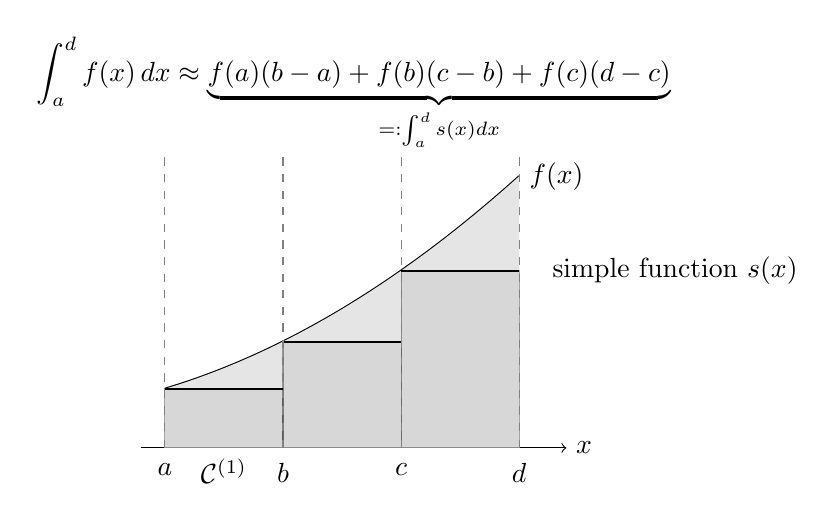
\begin{tikzpicture}[scale=1.5]
  
  \draw[->] (-0.2,0) -- (3.4,0) node[right] {$x$};
 
  
  \draw[thick,domain=0:3,smooth] plot(\x,{0.5+0.3*\x+0.1*\x*\x}) node[right] {$f(x)$};
  
  \fill[gray!20] (0,0) -- plot[domain=0:3] (\x,{0.5+0.3*\x+0.1*\x*\x}) -- (3,0) -- cycle;
  
  \draw[fill=gray!50,opacity=0.35] (0,0) rectangle (1,0.5);
  \node at (0.5,-0.2) {$\mathcal{C}^{(1)}$}; 
  \draw[fill=gray!50,opacity=0.35] (1,0) rectangle (2,0.9);
  \draw[fill=gray!50,opacity=0.35] (2,0) rectangle (3,1.5);
  
  \draw[thick] (0,0.5)--(1,0.5);
  \draw[thick] (1,0.9)--(2,0.9);
  \draw[thick] (2,1.5)--(3,1.5);
  \node[above left] at (0.8,0.5) {};
  
  \foreach \x in {0,1,2,3} \draw[dashed,gray] (\x,0) -- (\x,2.5);
  
  \node[anchor=north] at (0,-0.05) {$a$};
  \node[anchor=north] at (1,-0.05) {$b$};
  \node[anchor=north] at (2,-0.05) {$c$};
  \node[anchor=north] at (3,-0.05) {$d$};
  \node at (1.6,3.0) {$\displaystyle \int_a^d f(x)\,dx \approx \underbrace{f(a)(b-a) + f(b)(c-b)+f(c)(d-c)}_{=:\int_a^d s(x)dx}$};
  \node [anchor=west] at (3.2,1.5) {simple function $s(x)$};
\end{tikzpicture}
\end{figure}
 It is useful to think of the Lebesgue integral as a function that maps 
 an integrable function $f$ to the value of its integral, 
	$$ f \mapsto \int_{{\bf x}} f({\bf x}) d{\bf x}.$$ 
	The precise defintion of this function, including its domain 
	which are the integrable functions, is a corner-stone of 
	measure theory \cite[Ch. 1]{RudinBook}.
					\\ 
		See also: function.},
	first={Lebesgue integral},
	type=math, 
	firstplural={Lebesgue integral}
}

\newglossaryentry{cdf}
{name={cumulative distribution function (cdf)},
	description={The \index{cumulative distribution function (cdf)} cdf 
	$F^{(x)}\left(\eta\right)$ of a real-valued random variable (RV) $x$ is \cite{AshProbMeasure,papoulis}
	$$F^{(x)}\left(\eta\right) :=\mathbb{P}\left(x\leq \eta\right).$$
					\\ 
		See also: probability density function (pdf), probability distribution, random variable (RV).},
	first={cumulative distribution function (cdf)},
	firstplural={cumulative distribution functions (cdfs)}, 
	plural={cdfs}, 
	type=math,
	text={cdf} 
}

\newglossaryentry{weightedgraph}
{name={weighted graph},
	description={A graph\index{weghted graph} whose edges 
	are assigned numeric weights. Typically, these edge weights 
	are non-negative real numbers. For example, if a graph represents 
	a road network with nodes being intersections and edges representing 
	road segments, the edge weight could represent the capacity (measured 
	in maximum vehicles per hour) of the road segment \cite{NewmannBook}.  
					\\ 
		See also: graph.},
	first={weighted graph},
	type=math,
	firstplural={weighted graphs}, 
	plural={weighted graphs}, 
	text={weighted graph} 
}



\newglossaryentry{graph}
{name={graph},
 description={A graph\index{graph} $\mathcal{G}= \left( \mathcal{V},\mathcal{E}\right)$ 
 is a pair that consists of a node set $\mathcal{V}$ and an edge set $\mathcal{E}$. 
 In its most general form, a graph is specified by a map that 
 assigns each edge $e\in \mathcal{E}$ a pair of nodes \cite{RockNetworks}. 
 Unless specified otherwise, the term graph refers to an undirected graph. 
 A simple undirected graph is obtained by identifying each edge $e\in \mathcal{E}$ 
 with a set that contains two different nodes $\{i,i'\}$. 
 Weighted graphs also specify numeric weights $\edgeweight_{e}$ for each 
 edge $e\in \mathcal{E}$.
					\\ 
		See also: map, weights.},
 first={graph},
 text={graph}, 
 type=math
}

\newglossaryentry{uncertainty}
{name={uncertainty},
	description={In the context of machine learning (ML), uncertainty\index{uncertainty} refers to the presence of multiple 
		plausible outcomes or explanations based on available data. For example, the 
		prediction $\hat{h}({\bf x})$ produced by a trained machine learning (ML) model $\hat{h}$
	 	often reflects a range of possible values for the true label of a given data point. 
	 	The broader this range, the greater the associated uncertainty. Probability theory 
	 	allows us to represent, quantify, and reason about uncertainty in a 
	 	mathematically rigorous manner.
					\\ 
		See also: probabilistic model, risk, entropy, variance. },
	first={uncertainty},
	text={uncertainty}
}

\newglossaryentry{ucb}
{name={upper confidence bound (UCB)},
	description={Consider\index{upper confidence bound (UCB)} an machine learning (ML) 
		application that requires selecting, at each time step $t$, an action $\arm_{t}$ 
		from a finite set of alternatives $\actionset$. The utility of selecting action $\arm_{t}$ 
		is quantified by a numeric reward signal $r^{(\arm_{t})}$. 
		A widely used probabilistic model for this type of sequential decision-making problem 
		is the stochastic MAB setting \cite{Bubeck2012}. In this model, 
		the reward $r^{(a)}$ is viewed as the realization of a random variable (RV) 
		with unknown mean $\mu^{(a)}$. Ideally, we would always choose the 
		action with the largest expected reward $\mu^{(a)}$, but these 
		means are unknown and must be estimated from observed data. Simply 
		choosing the action with the largest estimate $\widehat{\mu}^{(a)}$ can 
		lead to suboptimal outcomes due to estimation uncertainty. The UCB strategy 
		addresses this by selecting actions not only based on their estimated means but 
		also by incorporating a term that reflects the uncertainty in these estimates—favoring 
		actions with a high-potential reward and high uncertainty. Theoretical guarantees 
		for the performance of UCB strategies, including logarithmic regret bounds, are established in \cite{Bubeck2012}.
					\\ 
		See also: optimism in the face of uncertainty, reward, MAB, uncertainty, regret.},
	first={upper confidence bound (UCB)},
	text={UCB} 
}

\newglossaryentry{mab}
{name={multiarmed bandit (MAB)},
	description={An MAB \index{multiarmed bandit (MAB)} problem is a precise 
	formulation of a sequential decision-making task under uncertainty. At each 
	discrete time step $t$, a learner selects one of several possible 
	actions—called arms—from a finite set $\actionset$. Pulling arm $a$ at time 
	$t$ yields a reward $r^{(a,t)}$ that is drawn from an unknown 
	probability distribution $\mathbb{P}\left(r^{(a,t)}\right)$. We obtain different classes 
	of MAB problems by placing different restrictions on this probability distribution. In the simplest 
	setting, the probability distribution $\mathbb{P}\left(r^{(a,t)}\right)$ does not depend on $t$. 
		Given an MAB problem, the goal is to construct machine learning (ML) methods that maximize the cumulative 
		reward over time by strategically balancing exploration (i.e., gathering information 
		about uncertain arms) and exploitation (i.e., selecting arms known to perform well). 
		MAB problems form an important special case of reinforcement learning (RL) problems \cite{Bubeck2012}, \cite{SuttonEd2}.
					\\ 
		See also: reward, regret.},
	first={MAB},
	text={MAB}
}



\newglossaryentry{optimism in the face of uncertainty}
{name={optimism in the face of uncertainty},
	description={machine learning (ML)\index{optimism in the face of uncertainty} methods learn model parameters ${\bf w}$ 
		according to some performance criterion $\bar{f}({\bf w})$. However, they usually 
		cannot access $\bar{f}({\bf w})$ directly but rely on an estimate (or approximation) 
		$f({\bf w})$ of $\bar{f}({\bf w})$. As a case in point, empirical risk minimization (ERM)-based methods use 
		the average loss on a given dataset (i.e., the training set) as an estimate 
		for the risk of a hypothesis. Using a probabilistic model, one can construct 
		a confidence interval $\big[ l^{({\bf w})},  u^{({\bf w})} \big]$ for each choice ${\bf w}$ for the model parameters.
		One simple construction is $l^{({\bf w})} :=f({\bf w}) - \sigma/2$, $u^{({\bf w})} :=f({\bf w})+ \sigma/2$, 
	    	with $\sigma$ being a measure of the (expected) deviation of $f({\bf w})$ from $\bar{f}({\bf w})$.
		We can also use other constructions for this interval as long as they ensure that $\bar{f}({\bf w}) \in\big[ l^{({\bf w})},  u^{({\bf w})} \big]$ 
		with a sufficiently high probability. An optimist chooses the model parameters 
		according to the most favorable—yet still plausible—value $\tilde{f}({\bf w}) :=l^{({\bf w})}$ 
		of the performance criterion (see Fig. \ref{fig_optimism_dict}). Two examples of machine learning (ML) methods that use such an optimistic 
		construction of an objective function are structural risk minimization (SRM) \cite[Ch. 11]{ShalevMLBook} and upper confidence bound (UCB) methods 
		for sequential decision making \cite[Sec. 2.2]{Bubeck2012}. 
		\begin{figure}[H]
			\begin{center}
			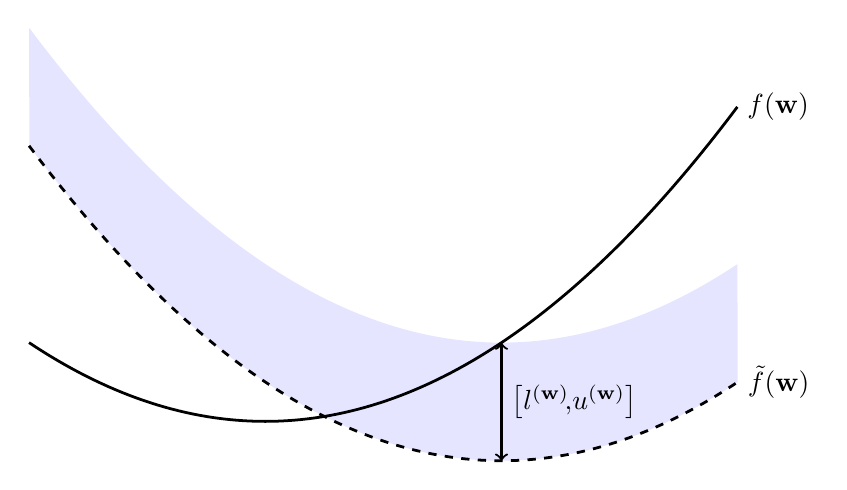
\begin{tikzpicture}[x=3cm, y=1cm]
  			
			\fill[blue!10] 
			(-1, 5) -- plot[domain=-2:1, samples=100] ({\x+1}, {\x*\x + 1}) -- 
			plot[domain=1:-2, samples=100] ({\x+1}, {\x*\x - 0.5}) -- cycle;
  			\node[anchor=west] at (2, 4) {$f({\bf w})$};
  			\draw[line width=1, domain=-2:1, samples=100,dashed] plot  ({\x+1}, {\x*\x -0.5}) node[right] {$\tilde{f}({\bf w})$};
   			\draw[line width=1, domain=-1:2, samples=100] plot ({\x}, {\x*\x});
  			\draw[<->, thick] (1, -0.5) -- (1, 1) node[midway, right] {$\big[ l^{({\bf w})}\!,\!u^{({\bf w})} \big]$};
			\end{tikzpicture}
			\caption{machine learning (ML) methods learn model parameters ${\bf w}$ by using some estimate of $f({\bf w})$ for 
			the ultimate performance criterion $\bar{f}({\bf w})$. Using a probabilistic model, one can use $f({\bf w})$ to 
			construct confidence intervals $\big[ l^{({\bf w})},  u^{({\bf w})} \big]$, which contain $\bar{f}({\bf w})$  
			with a high probability. The best plausible performance measure for a specific choice ${\bf w}$ of model parameters 
			is $\tilde{f}({\bf w}) :=l^{({\bf w})}$. \label{fig_optimism_dict}} 
			\end{center}
		\end{figure}
		See also: objective function, optimization method, gradient-based method, upper confidence bound (UCB).},
	first={optimism in the face of uncertainty},
	text={optimism in the face of uncertainty} 
}

\newglossaryentry{empgraph}
{name={federated learning network (FL network)},
	description={An federated learning (FL) network\index{federated learning network (FL network)} consists of 
		an undirected weighted graph $\mathcal{G}$. The nodes of $\mathcal{G}$ represent devices 
		that can access a local dataset and train a local model. The edges of $\mathcal{G}$ represent 
		communication links between devices as well as statistical similarities between their local datasets. 
		A principled approach to train the local models is generalized total variation minimization (GTVMin). The solutions of generalized total variation minimization (GTVMin) are local 
		model parameters that optimally balance the loss incurred on local datasets with their discrepancy 
		across the edges of $\mathcal{G}$.
	    			\\ 
		See also: federated learning (FL), graph, device, generalized total variation minimization (GTVMin).},
	first={federated learning network (FL network)},
	text={FL network} 
}

\newglossaryentry{norm}
{name={norm},
	description={A norm\index{norm} is a function that maps each (vector) element 
		of a vector space to a nonnegative real number. This function must be 
		homogeneous and definite, and it must satisfy the triangle inequality \cite{HornMatAnalysis}.
		\\
		See also: function, vector, vector space.},
	first={norm},
	text={norm} 
}

\newglossaryentry{dualnorm}
{name={dual norm},
	description={Every norm $\mleft\lVert \cdot \mright\rVert_{}$ defined on a Euclidean space $\mathbb{R}^{d}$ 
		has an associated dual norm, which is denoted by $\mleft\lVert \cdot \mright\rVert_{*}$ and defined as 
		$\mleft\lVert {\bf y}\mright\rVert_{*} :=\sup_{\Vert  {{\bf x}} \Vert{} \le 1} {\bf y}\,^{T} {\bf x}$. 
		The dual norm measures the largest possible inner product between ${\bf y}$ 
		and any vector in the unit ball of the original norm. For further details, see 
		\cite[Sec.~A.1.6]{BoydConvexBook}.
					\\ 
		See also: norm, Euclidean space, vector.},
	first={dual norm},
	text={dual norm}
}

\newglossaryentry{geometricmedian}
{name={geometric median (GM)},
	description={The GM\index{geometric median (GM)} of a set of input vectors ${\bf x}^{(1)}, \,\ldots, \,{\bf x}^{(m)}$ 
		in $\mathbb{R}^{d}$ is a point ${\bf z}\in \mathbb{R}^{d}$ that 
		minimizes the sum of distances to the vectors \cite{BoydConvexBook} such that 
		\begin{equation} 
			\label{equ_geometric_median_dict}
		{\bf z}\in \argmin_{{\bf y}\in \mathbb{R}^{d}} \sum_{r=1}^{m} \mleft\lVert {\bf y}- {\bf x}^{(r)} \mright\rVert_{2}.
		\end{equation} 
		Fig. \ref{opt_cond_GM_dict} illustrates a fundamental property of the GM:
		If ${\bf z}$ does not coincide with any of the input vectors, then the unit vectors pointing 
		from ${\bf z}$ to each ${\bf x}^{(r)}$ must sum to zero—this is the zero-subgradient  
		(optimality) condition for \eqref{equ_geometric_median_dict}. It turns out that the solution to 
		\eqref{equ_geometric_median_dict} cannot be arbitrarily pulled away from trustworthy input 
		vectors as long as they are the majority \cite[Th. 2.2]{Lopuhaae1991}.
	  	\begin{figure}[H]
  		\begin{center}
			\begin{tikzpicture}[scale=2, thick, >=stealth]

				\coordinate (w) at (3,0);
				\fill (w) circle (1.2pt) node[below right] {${\bf z}$};

				\coordinate (w2) at (0.5,0.3);
				\coordinate (w3) at (0.7,0.7);
				\fill (w2) circle (1pt) node[above left] {${\bf x}^{(1)}$};
				\fill (w3) circle (1pt) node[above left] {${\bf x}^{(2)}$};
			    \node[anchor=west] at ($(w2) +(-0.2,0.9)$) {\textbf{clean}};

				\draw[dashed] (w) -- (w2);
				\draw[dashed] (w) -- (w3);

				\draw[->, thick, red] (w) -- ($(w)!1cm!(w2)$) ;
				\draw[->, thick, red] (w) -- ($(w)!1cm!(w3)$) node[pos=0.9, right,yshift=7pt] {$\frac{{\bf x}^{(2)}- {\bf z}}{\mleft\lVert {\bf x}^{(2)}-{\bf z}\mright\rVert_{2}}$};

				\coordinate (w4) at (5,0.2);
				\node at (5,0.6) {\textbf{perturbed}};
				\fill (w4) circle (1pt) node[below left] {${\bf x}^{(3)}$};
				\draw[->, thick, red] (w) -- ($(w)!1cm!(w4)$) ;

		\end{tikzpicture}
		\caption{\label{opt_cond_GM_dict}
			Consider a solution ${\bf z}$ of \eqref{equ_geometric_median_dict} that does not coincide 
			with any of the input vectors. The optimality condition for \eqref{equ_geometric_median_dict} 
			requires that the unit vectors from ${\bf z}$ to the input vectors sum to zero.}
			\end{center}
		\end{figure}
		See also: vector, subgradient.},
	first={geometric median},
	text={GM}
}


\newglossaryentry{explanation}
{name={explanation}, plural={explanations},
	description={One approach to enhance the transparency of an machine learning (ML) method for its human user 
		is to provide an explanation\index{explanation} alongside the predictions delivered 
		by the method. Explanations can take different forms. For instance, they may 
        		consist of human-readable text or quantitative indicators, such as feature 
        		importance scores for the individual features of a given data point~\cite{Molnar2019}. 
	   	Alternatively, explanations can be visual—for example, intensity maps that highlight 
	   	image regions that drive the prediction \cite{GradCamPaper}. 
       		Fig.\ \ref{fig_explanation_dict} illustrates two types of explanations. The first 
       		is a local linear approximation $g({\bf x})$ of a nonlinear trained model 
       		$\hat{h}({\bf x})$ around a specific feature vector ${\bf x}'$, 
       		as used in the method LIME. 
        		The second form of explanation depicted in the figure is a sparse set of predictions 
       		$\hat{h}({\bf x}^{(1)}), \hat{h}({\bf x}^{(2)}), \hat{h}({\bf x}^{(3)})$ 
       		at selected feature vectors, offering concrete reference points for the user. 
	 	\begin{figure}[H]
	   		\begin{center}
	 		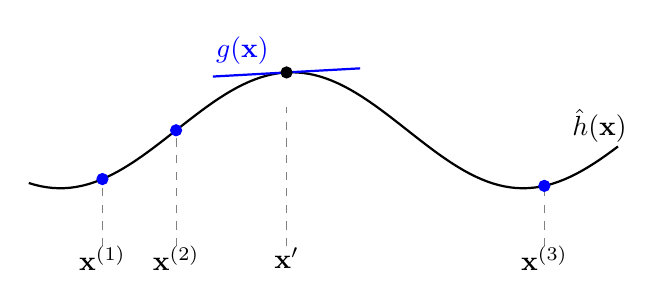
\begin{tikzpicture}[x=0.5cm]
	 		\begin{axis}[
	 			hide axis,
	 			xmin=-3, xmax=6,
	 			ymin=0, ymax=6,
	 			domain=0:6,
	 			samples=100,
	 			width=10cm,
	 			height=6cm,
	 			clip=false
	 		   ]
	 		
			\addplot[thick, domain=-2:6] {2 + sin(deg(x))} 
	   		     node[pos=0.9, above right, yshift=10pt] {$\hat{h}({\bf x})$};
	 		
	 		
	 		\addplot[blue, thick, domain=0.5:2.5] 
	 		{2 + sin(deg(1.5)) + cos(deg(1.5))*(x - 1.5)}
	 		node[pos=0.2, above] {$g({\bf x})$};
	 		
	 		\addplot[mark=*] coordinates {(1.5, {2 + sin(deg(1.5))})};
	 		    
			\addplot[dashed, gray] coordinates {(1.5,0) (1.5,2.4)};
	 		\node at (axis cs:1.5, -0.2) {${\bf x}'$};
	      		
	       		\addplot[mark=*,blue] coordinates {(-1, {2 + sin(deg(-1))})};
	       		\addplot[dashed, gray] coordinates {(-1,0) (-1,{2 + sin(deg(-1))})};
	       		\node at (axis cs:-1, -0.2) {${\bf x}^{(1)}$};
	 	   	\addplot[mark=*,blue] coordinates {(0, {2 + sin(deg(0))})};
	 	   	\addplot[dashed, gray] coordinates {(0,0) (0,{2 + sin(deg(0))})};
	 	   	\node at (axis cs:0, -0.2) {${\bf x}^{(2)}$};
	 	   	\addplot[mark=*,blue] coordinates {(5, {2 + sin(deg(5))})};
	 	   	\addplot[dashed, gray] coordinates {(5,0) (5,{2 + sin(deg(5))})};
	 	   	\node at (axis cs:5, -0.2) {${\bf x}^{(3)}$};
	
	
	
	
	
	
	 		\end{axis}
	
		\end{tikzpicture}
	 	\end{center}
	 	\caption{A trained model $\hat{h}({\bf x})$ can be explained 
	     	locally at some point ${\bf x}'$ by a linear approximation $g({\bf x})$. 
	     	For a differentiable $\hat{h}({\bf x})$, this approximation is 
	     	determined by the gradient $\nabla \hat{h}({\bf x}')$. Another 
	     	form of explanation could be the function values $\hat{h}\big({\bf x}^{(r)} \big)$ 
	     	for $r=1, 2, 3$. 
		\label{fig_explanation_dict}}
	 	\end{figure} 
		See also: machine learning (ML), prediction, feature, data point, classification.},
	first={explanation},
	text={explanation} 
}

\newglossaryentry{risk}
{name={risk},
	description={Consider\index{risk} a hypothesis $h$ used to predict the label 
		$y$ of a data point based on its features ${\bf x}$. We measure 
		the quality of a particular prediction using a loss function $L\left(({\bf x},y),h\right)$. 
		If we interpret data points as the realizations of independent and identically distributed (i.i.d.) random variables (RVs), 
		the $L\left(({\bf x},y),h\right)$ also becomes the realization 
		of a random variable (RV). The independent and identically distributed assumption (i.i.d.\ assumption) allows us to define the risk of a hypothesis 
		as the expected loss $\mathbb{E} \big\{L\left(({\bf x},y),h\right) \big\}$. 
		Note that the risk of $h$ depends on both the specific choice for the loss function and the 
		probability distribution of the data points.
					\\ 
		See also: independent and identically distributed (i.i.d.) random variable (RV), independent and identically distributed assumption (i.i.d.\ assumption), loss, probability distribution.},
	first={risk},
	text={risk} 
}

\newglossaryentry{actfun}
{name={activation function},
	description={Each\index{activation function} artificial neuron within an artificial neural network (ANN) is 
		assigned an activation function $\sigma(\cdot)$ that maps a weighted 
		combination of the neuron inputs $\feature_{1}, \,\ldots, \,\feature_{d}$ 
		to a single output value $a = \sigma\big(\weight_{1} \feature_{1}+\ldots+\weight_{d} \feature_{d} \big)$. 
		Note that each neuron is parameterized by the weights $\weight_{1}, \,\ldots, \,\weight_{d}$.
					\\ 
		See also: artificial neural network (ANN), activation, rectified linear unit (ReLU).},
	first={activation function},
	text={activation function} 
}

\newglossaryentry{distributedalgorithm}
{name={distributed algorithm},
	description={A\index{distributed algorithm} distributed algorithm is an algorithm designed for 
		a special type of computer, i.e., a collection of interconnected computing devices (or nodes). 
		These devices communicate and coordinate their local computations by exchanging 
		messages over a network \cite{IntroDistAlg}, \cite{ParallelDistrBook}. Unlike a classical algorithm, 
		which is implemented on a single device, a distributed algorithm is 
		executed concurrently on multiple devices with computational capabilities. 
		Similar to a classical algorithm, a distributed algorithm can be modeled as a 
		set of potential executions. However, each execution in the distributed setting involves 
		both local computations and message-passing events. A generic execution might look as 
		follows:
		\[
		\begin{array}{l}
			\text{Node 1: } {\rm input}_1, \,s_1^{(1)}, \,s_2^{(1)}, \,\ldots, \,s_{T_1}^{(1)}, \,{\rm output}_1; \\
			\text{Node 2: } {\rm input}_2, \,s_1^{(2)}, \,s_2^{(2)}, \,\ldots, \,s_{T_2}^{(2)}, \,{\rm output}_2; \\
			\quad \vdots \\
			\text{Node N: } {\rm input}_N, \,s_1^{(N)}, \,s_2^{(N)}, \,\ldots, \,s_{T_N}^{(N)}, \,{\rm output}_N.
		\end{array}
		\]
		Each device $i$ starts from its own local input and performs a sequence of 
		intermediate computations $s_{t}^{(i)}$ at discrete-time instants $t= 1, \,\dots, \,T_i$. 
		These computations may depend on both the previous local computations at the device 
		and the messages received from other devices. One important application of distributed 
		algorithms is in federated learning (FL) where a network of devices collaboratively trains a personal model 
		for each device. 
					\\ 
		See also: algorithm, device, event, federated learning (FL), model.
		},
	first={distributed algorithm}, 
	text={distributed algorithm}
}


\newglossaryentry{algorithm}
{name={algorithm}, plural={algorithms},
 	description={An\index{algorithm} algorithm is a precise, step-by-step specification for 
  		producing an output from a given input within a finite number of well-defined 
		computational steps \cite{Cormen:2022aa}. For example, an gradient-based method for linear regression 
		is an algorithm that explicitly describes how to map a given training set 
		into model parameters through a sequence of gradient steps. The precise form of 
		an algorithm depends on the available computational infrastructure. For example, if 
		this infrastructure allows to compute a inverse matrix matrix, then we can 
		define a linear regression algorithm using the normal equations. In contrast, if 
		the computational infrastructe does only allow for basic arithmetic (mulilication and addition), 
		the normal equations need to be somehow translated into a sequence of arithmetic 
		operations (e.g., as in gradient-based methods). 
		To study algorithms rigorously, we can represent (or approximate) them by different 
			mathematical structures \cite{Sipser2013}. One approach is to represent an algorithm 
			as a collection of possible executions. Each individual execution is then a 
			sequence of the form $${\rm input}, \,s_1, \,s_2, \,\ldots, \,s_T, \,{\rm output}.$$ 
			This sequence starts from an input and progresses via intermediate steps until an 
			output is delivered. Crucially, an algorithm encompasses more than just a mapping 
			from input to output; it also includes intermediate computational 
     		steps $s_1, \,\ldots, \,s_T$.
				\\ 
		See also: linear model, training set, model parameters, gradient step, model, stochastic.},
	first={algorithm},
	text={algorithm} 
}

\newglossaryentry{stochalgorithm}
{name={stochastic algorithm}, 
 plural={stochastic algorithms},
	description={A\index{stochastic algorithm} stochastic algorithm uses a random mechanism 
		during its execution. For example, stochastic gradient descent (SGD) uses a randomly selected subset of data points 
		to compute an approximation for the gradient of an objective function. We can represent a 
		stochastic algorithm by a stochastic processes, i.e., the possible execution sequence is the possible outcomes of 
		a random experiment \cite{BertsekasProb}, \cite{RandomizedAlgos}, \cite{Gallager13}.		
		\\ 
		See also: stochastic, algorithm, stochastic gradient descent (SGD), data point, gradient, objective function, stochastic process, 
		random experiment, optimization method, gradient-based method. },
	first={stochastic algorithm},
	text={stochastic algorithm} 
}

\newglossaryentry{batchlearning}
{name={batch learning},
	description={In batch learning\index{batch learning} (also known as offline learning), the machine learning (ML) model 
		is trained on the entire dataset in a single training iteration, instead of updating it incrementally as data arrive. 
		All available data are inputted into a learning algorithm, resulting in a model that can make predictions. 
		Since these datasets tend to be large, training is computationally expensive and time-consuming, 
		so it is typically performed offline. After learning, the model will be static and will not adapt to new data automatically. 
		Updating the model with new information requires retraining the model entirely. Once the model has been trained, 
		it is launched into production where it cannot be updated. Training a model can take many hours, so many models in production 
		settings are updated cyclically on a periodic schedule when the data distribution is stable. For example, a retail analytics team 
		could retrain their demand forecast model every Sunday using the previous week's sales data to predict next week's demand. 
		If a system needs to be constantly updated to rapidly changing data, such as in stock price prediction, a more adaptable solution 
		such as online learning is necessary.
		\\
		See also: batch, model, dataset, online learning. },
	first={batch learning}, 
	text={batch learning}
}

\newglossaryentry{onlinelearning}
{name={online learning},
	description={Some machine learning (ML) methods \index{online learning} are designed to process data in a sequential 
		manner, updating their model parameters one at a time, as new data points become available. 
		A typical example is time-series data, such as daily minimum and maximum temperatures 
		recorded by an Finnish Meteorological Institute (FMI) weather station. These values form a chronological sequence 
		of observations. During each time step $t$, online learning methods update (or refine)  
		the current hypothesis $h^{(t)}$ (or model parameters ${\bf w}^{(t)}$) 
		based on the newly observed data point ${\bf z}^{(t)}$. 
		\\ 
		See also: online gradient descent (online GD), online algorithm. },
	first={online learning},
	text={online learning} 
}

\newglossaryentry{onlinealgorithm}
{name={online algorithm},
	description={An\index{online algorithm} online algorithm processes input data incrementally, 
		receiving data points sequentially and making decisions or producing outputs (or decisions) immediately 
		without having access to the entire input in advance \cite{PredictionLearningGames}, \cite{HazanOCO}. 
		Unlike an offline algorithm, which has the entire input available from the start, an online algorithm 
		must handle uncertainty about future inputs and cannot revise past decisions. Similar to an 
		offline algorithm, we represent an online algorithm formally as a collection of possible 
		executions. However, the execution sequence for an online algorithm has a distinct structure as follows:
		$${\rm in}_{1}, \,s_1, \,{\rm out}_{1}, \,{\rm in}_{2}, \,s_2, \,{\rm out}_{2}, \,\ldots, \,{\rm in}_{T}, \,s_T, \,{\rm out}_{T}.$$ 
		Each execution begins from an initial state (i.e., \(\text{in}_{1}\)) and proceeds through alternating 
		computational steps, outputs (or decisions), and inputs. Specifically, at step \(t\), 
		the algorithm performs a computational step \(s_{t}\), generates an output \(\text{out}_{t}\), 
		and then subsequently receives the next input (data point) \(\text{in}_{t+1}\). A 
		notable example of an online algorithm in machine learning (ML) is online gradient descent (online GD), which incrementally 
		updates model parameters as new data points arrive. 
					\\ 
		See also: algorithm, data, data point, uncertainty, machine learning (ML), online gradient descent (online GD), model parameters, online learning.},
	first={online algorithm},
	text={online algorithm} 
}


\newglossaryentry{transparency}
{name={transparency},
	description={Transparency\index{transparency} is a fundamental requirement for 
		trustworthy artificial intelligence (trustworthy AI) \cite{HLEGTrustworhtyAI}. In the context of machine learning (ML) 
		methods, transparency is often used interchangeably with explainability 
		\cite{JunXML2020}, \cite{gallese2023ai}. However, in the broader scope of AI 
		systems, transparency extends beyond explainability and includes providing information 
		about the system’s limitations, reliability, and intended use. 
		In medical diagnosis systems, transparency requires disclosing the confidence level 
		for the predictions delivered by a trained model. In credit scoring, 
		AI-based lending decisions should be accompanied by explanations of 
		contributing factors, such as income level or credit history. These explanations 
		allow humans (e.g., a loan applicant) to understand and contest automated decisions. 
		Some machine learning (ML) methods inherently offer transparency. For example, logistic regression 
		provides a quantitative measure of classification reliability through the value $|h({\bf x})|$. 
		Decision trees are another example, as they allow human-readable decision rules \cite{rudin2019stop}.
		Transparency also requires a clear indication when a user is engaging with an AI system. 
		For example, AI-powered chatbots should notify users that they are interacting with an 
		automated system rather than a human. Furthermore, transparency encompasses comprehensive 
		documentation detailing the purpose and design choices underlying the AI system. 
		For instance, model datasheets \cite{DatasheetData2021} and AI system cards \cite{10.1145/3287560.3287596} 
		help practitioners understand the intended use cases and limitations of an AI system \cite{Shahriari2017}.
					\\ 
		See also: trustworthy artificial intelligence (trustworthy AI), explainability.},
	first={transparency}, 
	text={transparency} 
}



\newglossaryentry{sensattr}
{name={sensitive attribute}, plural={sensitive attributes},
	description={machine learning (ML)\index{sensitive attribute} revolves around learning a hypothesis map that allows 
		us to predict the label of a data point from its features. In some 
		applications, we must ensure that the output delivered by an machine learning (ML) system does 
		not allow us to infer sensitive attributes of a data point. Which part 
		of a data point is considered a sensitive attribute is a design 
		choice that varies across different application domains.
					\\ 
		See also: machine learning (ML), hypothesis, map, label, data point, feature.},
	first={sensitive attribute},
	text={sensitive attribute} 
}


\newglossaryentry{sbm}
{name={stochastic block model (SBM)},
	description={The\index{stochastic block model (SBM)} SBM is a 
		probabilistic generative model for an undirected graph $\mathcal{G}= \big( \mathcal{V}, \mathcal{E}\big)$ 
		with a given set of nodes $\mathcal{V}$ \cite{AbbeSBM2018}. In its most basic variant, 
		the SBM generates a graph by first randomly assigning each node $i\in \mathcal{V}$ to 
		a cluster index $\clusteridx_{i} \in \{1, \,\ldots, \,k\}$. A pair of different nodes in the 
		graph is connected by an edge with probability $p_{i,i'}$ that depends 
		solely on the labels $\clusteridx_{i}, \clusteridx_{i'}$. 
		The presence of edges between different pairs of 
		nodes is statistically independent.
					\\ 
		See also: model, graph, cluster, probability, label. },
	first={stochastic block model (SBM)},
	text={SBM} 
}

\newglossaryentry{deepnet}
{name={deep net}, plural={deep nets},
	description={A\index{deep net} deep net is an artificial neural network (ANN) with a (relatively) large number of 
		hidden layers. Deep learning is an umbrella term for machine learning (ML) methods that use a deep 
		net as their model \cite{Goodfellow-et-al-2016}.
				\\ 
		See also: artificial neural network (ANN), layer, machine learning (ML), model.},
	first={deep net},
	text={deep net} 
}



\newglossaryentry{baseline}
{name={baseline},
    description={Consider\index{baseline} some machine learning (ML) method that produces a learned 
    	hypothesis (or trained model) $\hat{h}\in \mathcal{H}$. We evaluate the quality of a trained model 
    	by computing the average loss on a test set. But how can we assess 
    	whether the resulting test set performance is sufficiently good? How can we 
    	determine if the trained model performs close to optimal such that there is little point 
   	in investing more resources (for data collection or computation) to improve it? 
    	To this end, it is useful to have a reference (or baseline) level against which 
    	we can compare the performance of the trained model. \\
	Such a reference value might be obtained from human performance, e.g., the misclassification rate of dermatologists 
    	who diagnose cancer from visual inspection of skin \cite{SkinHumanAI}. Another source for a baseline is an existing, 
    	but for some reason unsuitable, machine learning (ML) method. For example, the existing machine learning (ML) method 
    	might be computationally too expensive for the intended machine learning (ML) application. 
    	Nevertheless, its test set error can still serve as a baseline. Another, somewhat more principled, 
    	approach to constructing a baseline is via a probabilistic model. In many cases, given a probabilistic model $p({\bf x},y)$,  
    	we can precisely determine the minimum achievable risk among any hypotheses
    	(not even required to belong to the hypothesis space $\mathcal{H}$) \cite{LC}. \\
    	This minimum achievable risk (referred to as the Bayes risk) is the risk 
    	of the Bayes estimator for the label $y$ of a data point, given
    	its features ${\bf x}$. Note that, for a given choice of loss function, the 
    	Bayes estimator (if it exists) is completely determined by the probability distribution 
		$\mathbb{P}$ \cite[Ch. 4]{LC}. However, computing the Bayes estimator 
		and Bayes risk presents two main challenges. First, the probability distribution 
		$\mathbb{P}$ is unknown and 
		must be estimated from observed data. Second, even if $\mathbb{P}$ 
		were known, computing the Bayes risk exactly may be computationally 
		infeasible \cite{cooper1990computational}. 
	A widely used probabilistic model is the multivariate normal distribution $\left( {\bf x},y\right) \sim \mathcal{N}({\bm \mu},{\bm \Sigma})$ 
	for data points characterized by numeric features and labels.
	Here, for the squared error loss, the Bayes estimator is given by the posterior 
	mean $\mu_{y|{\bf x}}$ of the label $y$, given the 
	features ${\bf x}$ \cite{LC}, \cite{GrayProbBook}. The corresponding Bayes risk 
	is given by the posterior variance 
	$\sigma^{2}_{y|{\bf x}}$ (see Fig. \ref{fig_post_baseline_dict}).
	\begin{figure}[H]
		\begin{center}
		\begin{tikzpicture}
			
			\draw[->] (-1,0) -- (7,0) node[right] {$y$}; 
			
			\draw[thick,domain=-1:7,smooth,variable=\x] 
			  plot ({\x}, {2*exp(-0.5*((\x-3)^2))});
			
			\draw[dashed] (3,0) -- (3,2.5);
			\node[anchor=south] at ([yshift=-5pt] 3,2.5) {\small $\mu_{y|{\bf x}}$};
			
			\draw[<->,thick] (3-1,1) -- (3+1,1.0);
			\node[anchor=west] at ([yshift=2pt] 3,1.2) {\small $\sigma_{y|{\bf x}}$};
			
			
			
			  
  			\foreach \x in {0.5} {
				\node[red] at (\x, 0) {\bf \large $\times$};
 			 }
  			
  			\node[anchor=north] at (0.5,-0.2) {\small $\hat{h}({\bf x})$};
		  \end{tikzpicture}
		\end{center}
		\caption{If the features and the label of a data point are drawn 
		from a multivariate normal distribution, we can achieve the minimum risk (under squared error loss) 
		by using the Bayes estimator $\mu_{y|{\bf x}}$ 
		to predict the label $y$ of a data point with features ${\bf x}$. The corresponding 
		minimum risk is given by the posterior variance $\sigma^{2}_{y|{\bf x}}$. We can use 
		this quantity as a baseline for the average loss of a trained model $\hat{h}$. \label{fig_post_baseline_dict}}
		\end{figure}
		See also: Bayes risk, Bayes estimator.},
    first={baseline},
    text={baseline}
}

\newglossaryentry{kfoldcv}
{name={$k$-fold cross-validation ($k$-fold CV)},
 description={A method\index{$k$-fold cross-validation} for evaluating the 
 generalization gap of an empirical risk minimization (ERM)-based machine learning (ML) method. The idea is to divide dataset 
 $\mathcal{D}$ evenly into $k$ subsets (or folds) $\mathcal{D}^{(1)},\ldots,\mathcal{D}^{(k)}$
	\begin{figure}[htbp]
		\centering
	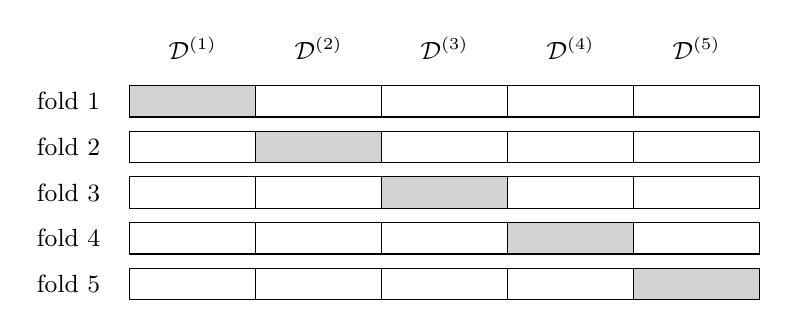
\begin{tikzpicture}[font=\small]
		\def\k{5}          
		\def\cellw{1.6}    
		\def\cellh{0.40}   
		\def\gap{0.18}     
		
		\foreach \i in {1,...,\k} {
			
			\pgfmathsetmacro{\y}{-(\i-1)*(\cellh+\gap)}
			
			\node[anchor=east] at (-0.25,\y+0.5*\cellh) {fold \i};
			
			\foreach \j in {1,...,\k} {
				\pgfmathsetmacro{\x}{(\j-1)*\cellw}
				\ifnum\i=\j
				\fill[gray!35] (\x,\y) rectangle ++(\cellw,\cellh);
				\draw (\x,\y) rectangle ++(\cellw,\cellh);
				\else
				\draw (\x,\y) rectangle ++(\cellw,\cellh);
				\fi
			}
		}
		
		\foreach \j in {1,...,\k} {
			\pgfmathsetmacro{\x}{(\j-1)*\cellw + 0.5*\cellw}
			\node[anchor=south] at (\x,\cellh+0.2) {$\mathcal{D}^{(\j)}$};
		}
	\end{tikzpicture}
	\caption{In $k$-fold cross-validation, the available dataset $\mathcal{D}$ is 
	evenly divided into $k$ folds $\mathcal{D}^{(1)},\ldots,\mathcal{D}^{(k)}$. Each fold is used once as a 
	validation set, while the remaining $k-1$ folds form the training set.		
	\label{fig_kfoldcv_dict}}
	\end{figure} 
	For each fold $b= 1, \,\ldots, \,k$, train the model on the 
	union of all folds except $\mathcal{D}^{(b)}$ and validate it on 
	$\mathcal{D}^{(b)}$. The overall performance is obtained by averaging 
	the validation results across all $k$ folds.
	\\ 
	See also: validation, validation error.},
	first={$k$-fold cross-validation ($k$-fold CV)},
	text={$k$-fold CV} 
}

\newglossaryentry{spectrogram}
{name={spectrogram},
	description={A\index{spectrogram} spectrogram represents the time-frequency distribution of the energy of a time signal $x(t)$.  
		Intuitively, it quantifies the amount of signal energy present within a specific time segment 
		$[t_{1},t_{2}] \subseteq \mathbb{R}$ and frequency interval $[f_{1},f_{2}]\subseteq \mathbb{R}$. 
		Formally, the spectrogram of a signal is defined as the squared magnitude of its 
		short-time Fourier transform (STFT) \cite{cohen1995time}.
        		Fig. \ref{fig:spectrogram_dict} depicts a time signal along with its spectrogram. 
		\begin{figure}[H]
			\centering
			\includegraphics[width=0.8\textwidth]{assets/spectrogram.png}
			\begin{minipage}{\textwidth}
				\vspace{3ex}
				\centering
				{\selectfont (a) \hspace{10em} (b)}
			\end{minipage}
			\caption{(a) A time signal consisting of two modulated Gaussian pulses. (b) An intensity 
			plot of the spectrogram.
			\label{fig:spectrogram_dict}}
		\end{figure}
        		The intensity plot of its spectrogram can serve as an image of a signal. A 
		simple recipe for audio signal classification is to feed this signal image 
		into deep nets originally developed for image classification and object detection \cite{Li:2022aa}. 
		It is worth noting that, beyond the spectrogram, several alternative representations exist 
		for the time-frequency distribution of signal energy \cite{TimeFrequencyAnalysisBoashash}, \cite{MallatBook}.
					\\ 
		See also: classification, deep net.}, 
	first={spectrogram},
	text={spectrogram} 
}

\newglossaryentry{graphclustering}
{name={graph clustering},
	description={Graph clustering\index{graph clustering} aims to 
		cluster data points that are represented as the nodes 
		of a graph $\mathcal{G}$. The edges of $\mathcal{G}$ represent 
		pairwise similarities between data points. We can sometimes
		quantify the extent of these similarities by an edge weight \cite{FlowSpecClustering2021}, \cite{Luxburg2007}.
					\\ 
		See also: graph, clustering, data point, edge weight. }, 
	first={graph clustering},
	text={graph clustering} 
}

\newglossaryentry{specclustering}
{name={spectral clustering},
	description={Spectral clustering\index{spectral clustering} is a particular instance of 
		graph clustering, i.e., it clusters data points 
		represented as the nodes $i=1, \,\ldots, \,n$ of a graph $\mathcal{G}$. 
		Spectral clustering uses the eigenvectors of the Laplacian matrix ${\bf L}^{(\mathcal{G})}$ 
		to construct feature vectors ${\bf x}^{(i)} \in \mathbb{R}^{d}$ 
		for each node (i.e., for each data point) $i=1, \,\ldots, \,n$. We can feed these feature vectors 
		into Euclidean space-based clustering methods, such as $k$-means 
		or soft clustering via Gaussian mixture model (GMM). Roughly speaking, the feature vectors of nodes 
		belonging to a well-connected subset (or cluster) of nodes in $\mathcal{G}$ are located 
		nearby in the Euclidean space $\mathbb{R}^{d}$ (see Fig. \ref{fig_lap_mtx_specclustering_dict}). 
		\begin{figure}[H]
			\begin{center}
				\begin{minipage}{0.4\textwidth}
			\begin{tikzpicture}
				
				\begin{scope}[every node/.style={circle, fill=black, inner sep=0pt, minimum size=0.3cm}]
					
					\node (1) at (0,0) {};
					\node (2) [below left=of 1, xshift=-0.2cm, yshift=-1cm] {};
					\node (3) [below right=of 1, xshift=0.2cm, yshift=-1cm] {};
					\node (4) [below=of 1, yshift=0.5cm] {}; 
				\end{scope}
				
				\draw (1) -- (2);
				\draw (1) -- (3);
				
				\node[above=0.2cm] at (1) {$i=1$};
				\node[left=0.3cm] at (2) {$2$};
				\node[right=0.3cm] at (3) {$3$};
				\node[below=0.2cm] at (4) {$4$};
				\node at (0,-4) {(a)};
			\end{tikzpicture}
				\end{minipage} 
				\hspace*{5mm}
				\begin{minipage}{0.4\textwidth}
					\begin{equation} 
						{\bf L}^{(\mathcal{G})}\!=\!
						\begin{pmatrix} 
							2 & -1 & -1 & 0 \\ 
							-1 & 1 & 0 & 0 \\  
							-1 & 0 & 1 & 0 \\ 
							0 & 0 & 0 & 0 
						\end{pmatrix}\!=\!\mathbf{V} {\bm \Lambda} \mathbf{V}\,^{T}  
						\nonumber
					\end{equation} 
					\begin{minipage}{\textwidth}
						\vspace{3ex}
						\centering
						{\selectfont (b)}
					\end{minipage}
				\end{minipage}
				\vspace*{20mm}\\
				\begin{minipage}{0.4\textwidth}
			\begin{tikzpicture}[scale=3]

					\draw[->] (-0.2, 0) -- (1.2, 0) node[right] {$v^{(1)}_{i}$};
					\draw[->] (0, -0.2) -- (0, 1.2) node[above] {$v^{(2)}_{i}$};







					\filldraw[blue] (0.577, 0) circle (0.03cm) node[above right] {$i=1,2,3$};
					\filldraw[blue] (0.577, 0) circle (0.03cm); 
					\filldraw[blue] (0.577, 0) circle (0.03cm); 
					\filldraw[red] (0, 1) circle (0.03cm) node[above right] {$4$};



					\node at (0.5,-0.5) {(c)};
			\end{tikzpicture}
				\end{minipage} 
    				\begin{minipage}{0.4\textwidth}
					\begin{align}
					& \mathbf{V} = \big( {\bf v}^{(1)},{\bf v}^{(2)},{\bf v}^{(3)},{\bf v}^{(4)} \big) \nonumber \\
					&	\mathbf{v}^{(1)}\!=\!\frac{1}{\sqrt{3}} \begin{pmatrix} 1 \\ 1 \\ 1 \\ 0 \end{pmatrix}, \,
					\mathbf{v}^{(2)}\!=\!\begin{pmatrix} 0 \\ 0 \\ 0 \\ 1 \end{pmatrix} \nonumber 
					\end{align}
					\begin{minipage}{\textwidth}
						\vspace{3ex}
						\centering
						{\selectfont (d)}
					\end{minipage}
				\end{minipage} 
				\caption{\label{fig_lap_mtx_specclustering_dict} (a) An undirected graph 
					$\mathcal{G}$ with four nodes $i=1,2,3,4$, each representing a data point. (b) The Laplacian matrix 
					${\bf L}^{(\mathcal{G})} \in \mathbb{R}^{4 \times 4}$ and its eigenvalue decomposition (EVD). 
					(c) A scatterplot of data points using the feature vectors 
					${\bf x}^{(i)} = \big( v^{(1)}_{i},v^{(2)}_{i} \big)\,^{T}$. 
					(d) Two eigenvectors ${\bf v}^{(1)},{\bf v}^{(2)} \in \mathbb{R}^{d}$ 
					corresponding to the eigenvalue $\lambda=0$ of the Laplacian matrix ${\bf L}^{(\mathcal{G})}$. } 
			\end{center}
		\end{figure}
		See also: clustering, graph clustering, Laplacian matrix, eigenvalue.
	\newpage}, 
	first={spectral clustering},
	text={spectral clustering} 
}

\newglossaryentry{flowbasedclustering}
{name={flow-based clustering},
	description={Flow-based clustering\index{flow-based clustering} groups the nodes 
		of an undirected graph by applying $k$-means clustering to nodewise 
		feature vectors. These feature vectors are built from network flows between 
		carefully selected sources and destination nodes \cite{FlowSpecClustering2021}. 
					\\ 
		See also: clustering, graph, $k$-means, feature vector.}, 
	first={flow-based clustering},
	text={flow-based clustering} 
}



\newglossaryentry{esterr}
{name={estimation error},
	description={Consider\index{estimation error} data points, each with feature vector ${\bf x}$ and label 
		$y$. In some applications, we can model the relation between the feature vector and the label
		of a data point as $y= \bar{h}({\bf x}) + \varepsilon$. Here, we 
		use some true underlying hypothesis $\bar{h}$ and a noise term $\varepsilon$, 
		which summarizes any modeling or labeling errors. The estimation error incurred by an machine learning (ML) 
		method that learns a hypothesis $\widehat{h}$, e.g., using empirical risk minimization (ERM), is defined as 
		$\widehat{h}({\bf x}) - \bar{h}({\bf x})$, for some feature vector. 
		For a parametric hypothesis space, which consists of hypothesis maps determined by 
		model parameters ${\bf w}$, we can define the estimation error as $\Delta {\bf w}= \widehat{{\bf w}} - \overline{{\bf w}}$ \cite{hastie01statisticallearning}, \cite{kay}.
					\\ 
		See also: data point, feature vector, label, hypothesis, machine learning (ML), empirical risk minimization (ERM), hypothesis space, map, model parameters.},
	first={estimation error},
	text={estimation error} 
}


\newglossaryentry{dob}
{name={degree of belonging}, 
	description={Degree of belonging\index{degree of belonging} is a number that indicates the extent to which a data point 
		belongs to a cluster \cite[Ch. 8]{MLBasics}. The degree of belonging can be 
		interpreted as a soft cluster assignment. Soft clustering methods can 
		encode the degree of belonging with a real number in the interval $[0,1]$. 
		Hard clustering is obtained as the extreme case when the degree of belonging 
		only takes on values $0$ or $1$.
					\\ 
		See also: data point, cluster, soft clustering, hard clustering.}, 
	first={degree of belonging},
	firstplural={degrees of belonging},
	plural={degrees of belonging},
	text={degree of belonging} 
}

\newglossaryentry{msee}
{name={mean squared estimation error (MSEE)},
	description={Consider\index{mean squared estimation error (MSEE)} an machine learning (ML) method that 
		learns model parameters $\widehat{{\bf w}}$ based on some dataset $\mathcal{D}$. 
		If we interpret the data points in $\mathcal{D}$ as independent and identically distributed (i.i.d.) realizations of a random variable (RV) ${\bf z}$, 
		we define the estimation error $\Delta {\bf w}:=\widehat{w} - \overline{{\bf w}}$. 
		Here, $\overline{{\bf w}}$ denotes the true model parameters of the probability distribution 
		of ${\bf z}$. The MSEE is 
		defined as the expectation $\mathbb{E} \big\{ \big\| \Delta {\bf w}\big\|^{2} \big\}$ of the 
		squared Euclidean norm of the estimation error \cite{LC}, \cite{kay}.
					\\ 
		See also: random variable (RV), estimation error, probabilistic model, squared error loss.},
	first={mean squared estimation error (MSEE)},
	text={MSEE} 
}

\newglossaryentry{gtvmin}
{name={generalized total variation minimization (GTVMin)},
	description={GTVMin\index{generalized total variation minimization (GTVMin)} is an instance of regularized empirical risk minimization (RERM) 
		using the generalized total variation (GTV) of local model parameters as a regularizer \cite{ClusteredFLTVMinTSP}.
					\\ 
		See also: regularized empirical risk minimization (RERM), generalized total variation (GTV), regularizer.},
	first={generalized total variation minimization (GTVMin)},
	text={GTVMin} 
}

\newglossaryentry{regression}
{name={regression},
	description={Regression\index{regression} problems revolve around the 
		prediction of a numeric label solely from the features of a data point \cite[Ch. 2]{MLBasics}.
					\\ 
		See also: prediction, label, feature, data point.},
	first={regression},
	text={regression} 
}

\newglossaryentry{acc}
{name={accuracy},
	description={Consider\index{accuracy} data points characterized by features ${\bf x}\in \mathcal{X}$ and 
		a categorical label $y$ that takes on values from a finite label space $\mathcal{Y}$. The 
		accuracy of a hypothesis $h: \mathcal{X}\rightarrow \mathcal{Y}$, when applied to the data points in a dataset 
		$\mathcal{D}= \big\{ \big({\bf x}^{(1)}, y^{(1)} \big), \,\ldots, \,\big({\bf x}^{(m)},y^{(m)}\big) \big\}$, 
		is then defined as $1 - (1/m)\sum_{r=1}^{m} L^{(0/1)}\left(\big({\bf x}^{(r)},y^{(r)}\big),h\right)$ 
		using the $0/1$ loss $L^{(0/1)}\left(\cdot,\cdot \right)$.
					\\ 
		See also: $0/1$ loss, loss, metric.},
	first={accuracy},
	text={accuracy} 
}


\newglossaryentry{expert}
{name={expert},
	description={machine learning (ML)\index{expert} aims to learn a hypothesis $h$ that accurately predicts the label 
		of a data point based on its features. We measure the prediction error using 
		some loss function. Ideally, we want to find a hypothesis that incurs minimal loss 
		on any data point. We can make this informal goal precise via the independent and identically distributed assumption (i.i.d.\ assumption) 
		and by using the Bayes risk as the baseline for the (average) loss of a hypothesis. 
		An alternative approach to obtaining a baseline is to use the hypothesis $h'$ learned 
		by an existing machine learning (ML) method. We refer to this hypothesis $h'$ as an expert \cite{PredictionLearningGames}. 
		Regret minimization methods learn a hypothesis
		that incurs a loss comparable to the best expert \cite{PredictionLearningGames}, \cite{HazanOCO}.
					\\ 
		See also: loss function, baseline, regret.},
	first={expert},
	text={expert} 
}

\newglossaryentry{nfl}
{name={networked federated learning (NFL)},
	description={NFL\index{networked federated learning (NFL)} refers 
		to methods that learn personalized models in a distributed fashion. These methods learn from local datasets 
		that are related by an intrinsic network structure.
					\\ 
		See also: model, local dataset, federated learning (FL).},
	first={networked federated learning (NFL)},
	text={NFL} 
}


\newglossaryentry{regret}
{name={regret},
	description={The regret\index{regret} of a hypothesis $h$ relative to 
		another hypothesis $h'$, which serves as a baseline, 
		is the difference between the loss incurred by $h$ and the loss 
		incurred by $h'$ \cite{PredictionLearningGames}. 
		The baseline hypothesis $h'$ is also referred to as an expert.
					\\ 
		See also: baseline, loss, expert.},
	first={regret},
	text={regret} 
}

\newglossaryentry{strcvx}
{name={strongly convex},
	description={A\index{strongly convex} continuously differentiable real-valued 
		function $f({\bf x})$ is strongly convex with coefficient $\sigma$ if $f({\bf y}) \geq f({\bf x}) + \nabla f({\bf x})\,^{T} ({\bf y}- {\bf x}) + (\sigma/2) \mleft\lVert {\bf y}- {\bf x}\mright\rVert_{2}^{2}$ \cite{nesterov04},\cite[Sec. B.1.1]{CvxAlgBertsekas}.
					\\ 
		See also: differentiable, function, convex.},
	first={strongly convex},
	text={strongly convex} 
}

\newglossaryentry{differentiable}
{name={differentiable},
	description={A\index{differentiable} real-valued function $f: \mathbb{R}^{d} \rightarrow \mathbb{R}$ 
		is differentiable if it can be approximated locally at any point by a linear function. 
		The local linear approximation at the point $\mathbf{x}$ is determined 
		by the gradient $\nabla f ( \mathbf{x})$ \cite{RudinBookPrinciplesMatheAnalysis}.
					\\ 
		See also: function, gradient.},
	first={differentiable},
	text={differentiable} 
}

\newglossaryentry{gradient}
{name={gradient}, plural={gradients},
	description={For\index{gradient} a real-valued function 
		$f: \mathbb{R}^{d} \rightarrow \mathbb{R}: {\bf w}\mapsto f({\bf w})$, 
		if a vector ${\bf g}$ exists such that 
		$\lim_{{\bf w}\rightarrow {\bf w}'} {f({\bf w}) - \big(f({\bf w}') + {\bf g}\,^{T} ({\bf w}- {\bf w}') \big) }/{\| {\bf w}- {\bf w}'\|}=0$, 
		it is referred to as the gradient of $f$ at ${\bf w}'$. If it exists, the gradient is unique and 
		denoted by $\nabla f({\bf w}')$ or $\nabla f({\bf w})\big|_{{\bf w}'}$ \cite{RudinBookPrinciplesMatheAnalysis}.
		\\
		See also: function, vector.},
	first={gradient},
	text={gradient} 
}

\newglossaryentry{subgradient}
{name={subgradient}, plural={subgradients},
	description={For\index{subgradient} a real-valued function $f: \mathbb{R}^{d} \rightarrow \mathbb{R}: {\bf w}\mapsto f({\bf w})$, 
		a vector ${\bf a}$ such that $f({\bf w}) \geq  f({\bf w}') +\big({\bf w}-{\bf w}' \big)\,^{T} {\bf a}$ is 
		referred to as a subgradient of $f$ at ${\bf w}'$ \cite{BertCvxAnalOpt}, \cite{BertsekasNonLinProgr}.
		\\
		See also: function, vector.},
	first={subgradient},
	text={subgradient} 
}

\newglossaryentry{fedprox}
{name={federated proximal (FedProx)},
	description={FedProx\index{federated proximal (FedProx)} refers to an iterative federated learning (FL) algorithm that alternates between separately 
		training local models and combining the updated local model parameters. In contrast to FedAvg, which uses 
		stochastic gradient descent (SGD) to train local models, FedProx uses a proximal operator for the training \cite{FedProx2020}.
					\\ 
		See also: federated learning (FL), algorithm, local model, model parameters, FedAvg, stochastic gradient descent (SGD), proximal operator.}, 
	first={FedProx}, 
	text={FedProx} 
}

\newglossaryentry{relu}
{name={rectified linear unit (ReLU)},
	description={The\index{rectified linear unit (ReLU)} ReLU is 
		a popular choice for the activation function of a neuron within an artificial neural network (ANN). It is defined 
		as $\sigma(z) = \max\{0,z\}$, with $z$ being the weighted input of the artificial 
		neuron.
					\\ 
		See also: activation function, artificial neural network (ANN).}, 
	first={rectified linear unit (ReLU)}, 
	text={ReLU} 
}

\newglossaryentry{hypothesis}
{name={hypothesis},
	description={A\index{hypothesis} hypothesis refers to a map (or function) $h: \mathcal{X}\rightarrow \mathcal{Y}$ 
		from the feature space $\mathcal{X}$ to the label space $\mathcal{Y}$. 
		Given a data point with features ${\bf x}$, we use a hypothesis 
		map $h$ to estimate (or approximate) the label $y$ 
		using the prediction $\hat{y} = h({\bf x})$. 
		\begin{figure}[htbp]
		\centering
			\begin{tikzpicture}[
 		  	>=Latex, node distance=2.0cm,
 		  	box/.style={draw, rounded corners=2pt, inner sep=6pt},
  		 	label/.style={font=\footnotesize},
  		 	thinline/.style={line width=0.6pt}
		 	]
		
		 	\node[minimum width=3.8cm, minimum height=1.6cm] (audio) {};
		 	
		 	\node[label] at (audio.north) [yshift=0mm] {audio samples ${\bf x}\in \mathbb{R}^{d}$};
		
		 	\begin{scope}
		 	
		 	\draw[thinline]
		 		($(audio.west)+(0.2,0)$) .. controls +(.3,.35) and +(-.3,.35) .. ++(0.8,0)
		 		.. controls +(.3,-.35) and +(-.3,-.35) .. ++(0.8,0)
		 		.. controls +(.3,.25) and +(-.3,.25) .. ++(0.8,0)
		 		.. controls +(.3,-.25) and +(-.3,-.25) .. ++(0.8,0);
		 	\end{scope}
		
		 	\node[box,right=1.0cm of audio, minimum width=2.2cm, minimum height=1.6cm] (model)
		 	{$h$};
		 	\draw[->,thinline] (audio) -- (model) ; 
		
		 	\node[right=1.0cm of model, minimum width=3.2cm, minimum height=1.6cm] (rating) {};
		 	\node[label, align=center] at ($(rating.north)+(0,-6mm)$)
		 		{};
		
		 	\coordinate (barL) at ($(rating.west)+(0.4,0)$);
		 	\coordinate (barR) at ($(rating.east)+(-0.4,0)$);
		 	\def\score{0.82}
		 	\coordinate (ptr) at ($(barL)!{\score}!(barR)$);
		 	
			
		 	\node[label, above=0pt of ptr] {$h({\bf x})=0.82 (\approx \mbox{Freddie level})$};
		 	\draw[->,thinline] (model) -- (rating);
		 	\end{tikzpicture}
			\caption{\label{fig:hypothesis_dict} A hypothesis $h: \mathcal{X}\rightarrow \mathcal{Y}$ maps the features 
				${\bf x}\in \mathcal{X}$ of a data point to a prediction $h({\bf x}) \in \mathcal{Y}$ of the label. 
				For example, the machine learning (ML) application \url{https://freddiemeter.withyoutube.com/} uses the samples of an audio 
				recording as features predict how closely a person’s singing resembles that of Freddie Mercury.
				}
		\end{figure}
		Machine learning (ML) is all about learning (or finding) a hypothesis map $h$ 
		such that $y\approx h({\bf x})$ for any data point 
		(with features ${\bf x}$ and label $y$). Practical machine learning (ML) methods, 
		limited by finite computational resources, must restrict learning to a subset of all possible 
		hypothesis maps. This subset is called the hypothesis space or simply the model underlying 
		the method.
					\\ 
		See also: map, function, prediction, model.},
	first={hypothesis},
	firstplural={hypotheses},
	plural={hypotheses},
	text={hypothesis}  
}

\newglossaryentry{effdim}
{name={effective dimension},
	description={The\index{effective dimension} effective dimension $d_{\rm eff} \left( \mathcal{H}\right)$ of 
		an infinite hypothesis space $\mathcal{H}$ is a measure of its size. Loosely speaking, the 
		effective dimension is equal to the effective number of independent tunable model parameters. 
		These parameters might be the coefficients used in a linear map or the 
		weights and bias terms of an artificial neural network (ANN).
					\\ 
		See also: hypothesis space, model parameters, artificial neural network (ANN).},
	first={effective dimension},
	text={effective dimension}  
}

\newglossaryentry{labelspace}
{name={label space},
	description={
		In a machine learning (ML) application\index{label space}, each data point is described by a 
		set of features together with an associated label. 
		The set of all admissible label values is called the label space,
		denoted by $\mathcal{Y}$. Importantly, $\mathcal{Y}$ may include values that no 
		observed data point has as its label value. 
		To a large extent, the choice of $\mathcal{Y}$ is up to the machine learning (ML) engineer 
		and depends on the problem formulation. Fig.~\ref{fig_label_spaces_dict} shows some examples 
		of label spaces that are commonly used in machine learning (ML) applications.
		\begin{figure}[H]
		\centering
		\begin{tikzpicture}[>=Stealth, font=\small]
			
			\begin{scope}[shift={(0,0)}]
				\draw[->] (-2,0) -- (2,0);
				\node[below=6pt] at (0,-0.7) {(a) $\mathcal{Y}\!=\!\mathbb{R}$ (regression)};
			\end{scope}
			
			\begin{scope}[shift={(7,0)}]
				
				\fill[gray!20] (-1,-0.5) rectangle (1,0.5);
				\draw[->] (-2,0) -- (2,0);
				\draw[->] (0,-1) -- (0,1);
				\node[below=6pt] at (0,-0.7) {(b) $\mathcal{Y}\!=\!\mathbb{R}^{2}$ (multi-label regression)};
			\end{scope}
			
			\begin{scope}[shift={(0,-3)}]
				\fill (-1,0) circle (1.2pt) node[below=2pt] {\text{``hot''}};
				\fill ( 1,0) circle (1.2pt) node[below=2pt] {\text{``cold''}};
				\node[below=14pt] at (0,-0.7) {(c) $|\mathcal{Y}|=2$ Binary classification};
			\end{scope}
			
			\begin{scope}[shift={(7,-3)}]
				\node[circle, inner sep=1pt, draw] (n1) at (-1.5,0) {};
				\node[circle, inner sep=1pt, draw] (n2) at (-0.5,0) {};
				\node[circle, inner sep=1pt, draw] (n3) at ( 0.5,0) {};
				\node[circle, inner sep=1pt, draw] (n4) at ( 1.5,0) {};
				\draw[->] (n1) -- (n2);
				\draw[->] (n2) -- (n3);
				\draw[->] (n3) -- (n4);
				\node[below=2pt of n1] {1};
				\node[below=2pt of n2] {2};
				\node[below=2pt of n3] {3};
				\node[below=2pt of n4] {4};
				\node[below=14pt] at (0,-0.7) {(d) $\mathcal{Y}\!=\!\{1,2,3,4\}$ (ordinal regression)};
			\end{scope}
		\end{tikzpicture}
		\caption{\label{fig_label_spaces_dict}	Examples of label spaces and corresponding flavours of 
		machine learning (ML).}
		\end{figure}
		The choice of label space $\mathcal{Y}$ determines the flavour of machine learning (ML) methods 
		appropriate for the application at hand. Regression methods use the $\mathcal{Y}= \mathbb{R}$ while binary classification methods 
		use a label space $\mathcal{Y}$ that consists of two different 
		elements, i.e., $|\mathcal{Y}|=2$. Ordinal regression methods use a finite, ordered set of 
		label values, e.g., $\mathcal{Y}= \{1,2,3,4\}$ with the natural ordering $1 < 2 < 3 < 4$. 
					\\ 
		See also:  data point,label, regression, classification.}, 
	first={label space},
	text={label space}  
}

\newglossaryentry{prediction}
{name={prediction}, plural={predictions},
	description={A\index{prediction} prediction is an estimate or approximation for some 
		quantity of interest. Machine learning (ML) revolves around learning or finding a hypothesis map $h$ 
		that reads in the features ${\bf x}$ of a data point and delivers a prediction 
		$\widehat{y} :=h({\bf x})$ for its label $y$.
					\\ 
		See also: machine learning (ML), hypothesis, map, feature, data point, label.},
	first={prediction},
	text={prediction}  
}

\newglossaryentry{empiricaldistribution}
{name = {empirical distribution},
 text = {empirical distribution},
plural = {empirical distributions},
first = {empirical distribution},
description = {Consider a dataset 
 $\mathcal{D}= \{ {\bf x}^{(1)},\ldots, {\bf x}^{(m)}\}$ 
  consisting of $m$ distinct data points, each characterized by 
  the feature vector ${\bf x}^{(r)} \in \mathcal{X}$ for $r= 1, \ldots, m$. 
  For a given $\sigma$-algebra $\Sigma$ over the feature space 
  $\mathcal{X}$, the empirical distribution \index{empirical distribution} 
  of $\mathcal{D}$ is the probability distribution $\mathbb{P}^{(\mathcal{D})}$ defined via 
   $$\mathbb{P}^{(\mathcal{D})}(\mathcal{A}) = (1/m) \big| \big\{ r: {\bf x}^{(r)} \in \mathcal{A} \big\} \big|, 
	\quad \text{for any } \mathcal{A} \in \Sigma.
	$$
	In other words, the empirical distribution assigns to any measurable set 
	$\mathcal{A} \in \Sigma$ the fraction of data points in $\mathcal{D}$ 
	that fall into $\mathcal{A}$. If the feature space is ordered, the empirical 
	distribution can also be characterized by its empirical cumulative distribution function (cdf)
	$$F^{(\mathcal{D})}\left({\bf x}\right) = 
	(1/m) \big| \big\{ r: {\bf x}^{(r)} \preceq {\bf x}\big\} \big|, 
	\quad \text{for any } {\bf x}\in \mathcal{X},$$
	where $\preceq$ denotes the ordering relation on $\mathcal{X}$.
	\begin{figure}[H]
	\begin{center}
	\begin{tikzpicture}[>=stealth, thick,y=2cm]
		\foreach \x/\p in {1/0.3, 4/0.7}
		{
		\draw[gray] (\x,0) -- (\x,\p);
		
		\fill[blue] (\x,\p) circle (2pt);
		}
		\node[anchor=south,align=center] at (1,0.3) {\small $p^{(\mathcal{D})}\left(\star\right)=3/10$};
		\node[anchor=north] at (1,0) {\small $\star$};
		\node[anchor=north] at (4,0) {\small $\otimes$};
			
		\node[anchor=west,text width=11cm] at (-1.2,-0.80) {
			$\mathcal{D}= (\star,\star,\star,\otimes,\otimes,\otimes,\otimes,\otimes,\otimes,\otimes)$
		};
	\end{tikzpicture}
    \end{center}
	\caption{A dataset $\mathcal{D}$ consisting of $m=10$ data points, each 
	characterized by a value from the finite feature space $\mathcal{X}= \{\star, \otimes\}$. 
	The empirical probability mass function (pmf) $p^{(\mathcal{D})}\left({\bf x}\right)$ assigns to each 
		possible value ${\bf x}\in \mathcal{X}$ the fraction of data points 
		in $\mathcal{D}$ whose feature takes on this value. Here, three out of 
        ten data points take on the feature value $\star$, resulting 
		in $p^{(\mathcal{D})}\left(\star\right) = 3/10$. \label{fig_empirical_pmf_dict}}
	\end{figure}
	If the feature space $\mathcal{X}$ is finite, 
	the empirical distribution of $\mathcal{D}$ can also be characterized by 
	the empirical probability mass function (pmf)  
	$$p^{(\mathcal{D})}\left({\bf x}\right) = 
	(1/m) \big| \big\{ r: {\bf x}^{(r)} = {\bf x}\big\} \big|, 
	\quad \text{for any } {\bf x}\in \mathcal{X}.$$
	\\
        See also: probability distribution, $\sigma$-algebra.
    },
    type = {math}
}




\newglossaryentry{histogram}
{name={histogram},
	description={Consider\index{histogram} a dataset $\mathcal{D}$ that consists of 
	$m$ data points ${\bf z}^{(1)}, \,\ldots, \,{\bf z}^{(m)}$, 
	each of them belonging to some cell $[-U,U] \times \ldots \times [-U,U] \subseteq \mathbb{R}^{d}$ with side 
		length $U$. We partition this cell evenly into smaller elementary cells with side 
		length $\Delta$. The histogram of $\mathcal{D}$ assigns each elementary cell to 
		the corresponding fraction of data points in $\mathcal{D}$ that fall into this 
		elementary cell. A visual example of such a histogram is provided in Fig. \ref{fig:histogram_dict}.\\
		\begin{figure}[H]
		\centering
		\begin{tikzpicture}
		\pgfplotsset{compat=1.18}
		\begin{axis}[
		    ybar,
		    ymin=0,
		    ymax=6,
		    bar width=22pt,
		    width=10cm,
		    height=6cm,
		    xlabel={Value},
		    ylabel={Frequency},
		    ytick={1,2,3,4,5,6},
		    xtick={1,2,3,4,5},
		    xticklabels={{[0,1)}, {[1,2)}, {[2,3)}, {[3,4)}, {[4,5)}},
		    enlarge x limits=0.15,
		    title={Histogram of Sample Data}
			]
		\addplot+[fill=blue!40] coordinates {(1,2) (2,5) (3,4) (4,3) (5,1)};
		\end{axis}
		\end{tikzpicture}
		\caption{A histogram consists of the fractions of data points that 
		fall within different value ranges (i.e., bins). Each bar height shows 
		the count of samples in the corresponding interval.}
		\label{fig:histogram_dict}
		\end{figure}
		See also: dataset, data point, sample.},
	first={histogram},
	text={histogram}  
}

\newglossaryentry{bootstrap}
{name={bootstrap},
	description={For\index{bootstrap} the analysis of machine learning (ML) methods, it is often 
	    useful to interpret a given dataset $\mathcal{D}= \big\{ {\bf z}^{(1)}, \,\ldots, \,{\bf z}^{(m)}\big\}$ 
		as (realizations of) a collection of independent and identically distributed (i.i.d.) random variables (RVs) with 
		common probability distribution $\mathbb{P}$. In practice, the probability distribution $\mathbb{P}$ 
		is unknown and must be estimated from $\mathcal{D}$. The idea of the bootstrap 
		method is to use the empirical distribution $\mathbb{P}^{(\mathcal{D})}$ 
		of $\mathcal{D}$ as an estimator for $\mathbb{P}$ \cite{hastie01statisticallearning}, 
		$$ (1/m) \big| r: {\bf z}^{(1)} \in \mathcal{A} \big| \approx \mathbb{P}\left(\mathcal{A}\right).$$
		Repeatedly sampling from the empirical distribution, which is equivalent 
		to sampling with replacement from $\mathcal{D}$ \cite{BoostrapBook}, 
		results in new datasets $\mathcal{D}^{(1)}, \ldots, \mathcal{D}^{(B)}$, each containing 
		$m$ data points. We then use each of 
		those datasets for model training (e.g., via empirical risk minimization (ERM)), 
		resulting in the learned hypotheses
		$\widehat{h}^{(1)}, \ldots, \hat{h}^{(B)}.$ 
        We can use these learned hypotheses to estimate important characteristics 
		of a machine learning (ML) method such as bias, variance or generalization gap. \cite{hastie01statisticallearning}.
		\\
		See also: independent and identically distributed (i.i.d.), random variable (RV), probability distribution, histogram.},
	first={bootstrap},
	text={bootstrap}  
}

\newglossaryentry{featurespace}
{name={feature space},
	description={The\index{feature space} feature space of a given machine learning (ML) application 
		or method is constituted by all potential values that the feature vector of a data point can take on. 
		For data points described by a fixed number $d$ of numerical features, 
		a common choice for the feature space is the Euclidean space $\mathbb{R}^{d}$. 
		However, the mere presence of $d$ numeric features does not imply that $\mathbb{R}^{d}$ 
		is the most appropriate representation of the feature space. Indeed, the numerical features  
		might be assigned to data points in a largely arbitrary or random manner, resulting 
		in data points that are randomly scattered throughout $\mathbb{R}^{d}$ 
		without any meaningful geometric structure. Feature learning methods try to learn a 
		transformation of the original (potentially non-numeric) features to ensure a 
		more meaningful arrangement of data points in $\mathbb{R}^{d}$. 
		Three examples of feature spaces are shown in Fig. \ref{fig_featurespace_dict}.
		\begin{figure}[H]
			\centering
			\begin{tikzpicture}[scale=0.6]
			
			\begin{scope}[xshift=0cm]
  				
 	 			\draw[->] (-0.5, 0) -- (3.5, 0) node[right] {$x_1$};
  				
  				\foreach \x/\lbl in {0.5/${\bf x}^{(1)}$, 1.5/${\bf x}^{(2)}$, 2.8/${\bf x}^{(3)}$}
    				\filldraw[blue] (\x,0) circle (2pt) node[above] {\lbl};
  				
  				\node at (1.5, -4.0)  {$\mathcal{X}^{(1)}$};
				\node at (1.5, -6) {(a)};
			\end{scope}
			
			\begin{scope}[xshift=8cm]
  				
  				\draw[thick] (0,0) circle (1.8);
  				\fill[gray!5] (0,0) circle (1.8);
  				
  				\filldraw[red] (0.8, 0.9) circle (2pt) node[anchor=south west] {${\bf x}^{(1)}$};
  				\filldraw[blue] (-1.2, 0.5) circle (2pt) node[anchor=south east] {${\bf x}^{(2)}$};
  				\filldraw[green!50!black] (0.3, -1.4) circle (2pt) node[anchor=north west] {${\bf x}^{(3)}$};
  				
  				\node at (0.5, -4) {$\mathcal{X}^{(2)}$};
				\node at (0.5, -6) {(b)};
			\end{scope}
			
			\begin{scope}[xshift=14cm, yshift=0.3cm]
  				
 	 			\filldraw[blue!60] (0,0) circle (2pt) node[anchor=north east] {${\bf x}^{(1)}$};
 	 			\filldraw[red!70] (2,1.2) circle (2pt) node[anchor=south west] {${\bf x}^{(2)}$};
  				\filldraw[green!50!black] (1,2.5) circle (2pt) node[anchor=south east] {${\bf x}^{(3)}$};
  				\filldraw[orange!80] (3,2.5) circle (2pt) node[anchor=south west] {${\bf x}^{(4)}$};
  				
  				\draw[-] (0,0) -- (2,1.2);
  				\draw[-] (2,1.2) -- (1,2.5);
  				\draw[-] (1,2.5) -- (3,2.5);
  				
  				\node at (1.5, -4.2) {$\mathcal{X}^{(3)}$};
				\node at (1.5, -6.2) {(c)};
			\end{scope}
			\end{tikzpicture}
		\caption{Three different feature spaces. (a) A linear space $\mathcal{X}^{(1)} = \mathbb{R}$. (b) A 
		bounded convex set $\mathcal{X}^{(2)} \subseteq \mathbb{R}^{2}$. (c) A discrete space 
		$\mathcal{X}^{(3)}$ whose elements are nodes of an undirected graph. \label{fig_featurespace_dict}}
		\end{figure}
		See also: feature vector, Euclidean space.},
	first={feature space},
	text={feature space}  
}


\newglossaryentry{missingdata}
{name={missing data},
	description={Consider\index{missing data} a dataset constituted by data points collected via 
		some physical device. Due to imperfections and failures, some of the feature 
		or label values of data points might be corrupted or simply missing. 
		Data imputation aims to estimate these missing values \cite{Abayomi2008DiagnosticsFM}. 
		We can interpret data imputation as an machine learning (ML) problem where the label of a data point is 
		the value of the corrupted feature.
				\\
		See also: feature, label. },
	first={missing data},
	text={missing data}  
}

\newglossaryentry{dataimputation}
{name={data imputation},
	description={See\index{data imputation} missing data.},
	first={data imputation},
	text={data imputation}  
}



\newglossaryentry{psd}
{name={positive semi-definite (psd)},
	description={A\index{positive semi-definite (psd)} (real-valued) symmetric matrix $\mathbf{Q}= \mathbf{Q}\,^{T} \in \mathbb{R}^{d\times d}$ 
	 	is referred to as psd if ${\bf x}\,^{T} \mathbf{Q}{\bf x}\geq 0$ for every vector ${\bf x}\in \mathbb{R}^{d}$. 
	 	The property of being psd can be extended from matrices to (real-valued) 
	 	symmetric kernel maps $K: \mathcal{X}\times \mathcal{X}\rightarrow \mathbb{R}$ 
	 	(with $K({\bf x},{\bf x}') = K({\bf x}',{\bf x})$)
	 	as follows: For any finite set of feature vectors ${\bf x}^{(1)}, \,\ldots, \,{\bf x}^{(m)}$, 
	 	the resulting matrix $\mathbf{Q}\in \mathbb{R}^{m\times m}$ with 
		entries $Q_{r,r'} = K\big({\bf x}^{(r)},{\bf x}^{(r')}\big)$ 
		is psd \cite{LearningKernelsBook}.
			\\
		See also: matrix, vector, kernel, map, feature vector.},
	first={positive semi-definite (psd)},
	text={psd}  
}

\newglossaryentry{feature}
{name={feature}, plural={features},
	description={A\index{feature} feature of a data point is one of its properties 
	    that can be measured or computed easily without the need for human supervision. 
		For example, if a data point is a digital image (e.g., stored as a \texttt{.jpeg} file), 
		then we could use the red–green–blue (RGB) intensities of its pixels as features. 
		\begin{figure}
		\centering
		\begin{tikzpicture}[scale=1]
		
		\draw[thick, blue, domain=0:6.28, smooth, variable=\x] 
			plot ({\x}, {sin(\x r)});
		
		\foreach \x [count=\i] in {0,0.5,...,6.28} {
			\fill[red] (\x, {sin(\x r)}) circle (2pt);
			
			\ifnum\i=1
				\node[above left] at (\x, {sin(\x r)}) {$x_1$};
			\fi
			\ifnum\i=2
				\node[above left] at (\x, {sin(\x r)}) {$x_2$};
			\fi
		}
		\end{tikzpicture}
		\caption{An audio signal (blue waveform) and its discretized signal samples (red dots) which 
		can be used as its features $x_{1},\ldots,x_{d}$. \label{fig:audio_features_dict}}
		\end{figure}
		Another example is shown in Fig.\ \ref{fig:audio_features_dict}, where the the signal 
		samples of a finite-duration audio signal are used as its features.
		Domain-specific synonyms for the term feature are "covariate," "explanatory variable," 
		"independent variable," "input (variable)," "predictor (variable)," or "regressor" \cite{Gujarati2021}, \cite{Dodge2003}, \cite{Everitt2010}. 
				\\
		See also: data point.}, 
	first={feature},
	text={feature}  
}

\newglossaryentry{featurevec}
{name={feature vector}, plural={feature vectors},
	description={Feature vector refers to a\index{feature vector} vector ${\bf x}= \big(x_{1}, \,\ldots, \,x_{d}\big)\,^{T}$ 
		whose entries are individual features $x_{1}, \,\ldots, \,x_{d}$. Many machine learning (ML) methods 
		use feature vectors that belong to some finite-dimensional Euclidean space $\mathbb{R}^{d}$. 
		For some machine learning (ML) methods, however, it can be more convenient to work with feature 
		vectors that belong to an infinite-dimensional vector space (e.g., see kernel method). 
			\\
		See also: feature, vector, machine learning (ML), Euclidean space, vector space.}, 
	first={feature vector},
	text={feature vector}  
}


\newglossaryentry{label}
{name={label}, plural={labels},
	description={A\index{label} higher-level fact or quantity of interest associated 
	with a data point. For example, if the data point is an image, the label 
	could indicate whether the image contains a cat or not. Synonyms for label, commonly 
	used in specific domains, include "response variable," "output variable," and "target" \cite{Gujarati2021}, \cite{Dodge2003}, \cite{Everitt2010}.
				\\
		See also: data point, label space.},
	first={label},
	text={label}  
}


\newglossaryentry{data}
{name={data},
 description={In the context of machine learning (ML), the term 
 data\index{data} is often used synonymously with dataset
  \cite{Everitt2010,OxfordStatisticsDictionary}. 
  The ISO/IEC 2382:2015 standard defines data as a \emph{re-interpretable representation of 
  information in a formalized manner suitable for communication, interpretation, 
  or processing} \cite{ISO2382}. 
  \\
  See also: dataset, data point, sample.}, 
  text={data}
}
		
\newglossaryentry{dataset}
{name={dataset}, plural={datasets},
	description={A\index{dataset} dataset is a set of distinct data points. 
	Strictly speaking, a dataset is an unordered collection of data points 
	that does not contain any repetitions. However, in machine learning (ML) literature, the 
	term dataset is often used as a synonym for a sample, i.e., 
	a sequence (or finite list) of data points and may contain repetitions. 
	machine learning (ML) methods use datasets for model training and validation. 
	The notion of a dataset is broad: data points may represent concrete 
	physical entities (such as humans or animals) or abstract objects (such as numbers). 
	For illustration, Fig.~\ref{fig_cows_dataset_dict} depicts a dataset whose 
	data points are cows.	
		\begin{figure}[H]
			\begin{center}
			\label{fig:cowsintheswissalps_dict}
			\includegraphics[width=0.5\textwidth]{assets/CowsAustria.jpg}
		  	\end{center}
			\caption{\label{fig_cows_dataset_dict}A cow herd somewhere in the Alps.}
	 	\end{figure}
		Quite often, an machine learning (ML) engineer does not have direct access to the underlying dataset. 
		For instance, accessing the dataset in Fig.~\ref{fig_cows_dataset_dict} would require 
		visiting the cow herd. In practice, we work with a more convenient 
		representation (or approximation) of the dataset. Various mathematical models 
		have been developed for this purpose \cite{silberschatz2019database}, \cite{abiteboul1995foundations}, 
		\cite{hoberman2009data}, \cite{ramakrishnan2002database}. One of the most widely used is 
		the relational model, which organizes data as a table (or relation) 
		\cite{codd1970relational}, \cite{silberschatz2019database}. A table consists of 
		rows and columns: each row corresponds to a single data point, while each 
		column represents a specific attribute of a data point. 
		machine learning (ML) methods typically interpret these attributes as features 
		or as a label of a data point. As an illustration, 
		Table~\ref{tab:cowdata_dict} shows a relational representation of the 
		dataset from Fig.~\ref{fig_cows_dataset_dict}. In the relational model, 
		the order of rows is immaterial, and each attribute (column) is associated with a 
		domain that specifies the set of admissible values. In machine learning (ML) applications, 
		these attribute domains correspond to the feature space and the label space.
		\begin{table}[H]
			\refstepcounter{table}
			\caption*{
				\centering 
				\scshape TABLE \thetable \\[0.5ex]
				\scshape A Relation (or Table) That Represents the Dataset in Fig. \ref{fig_cows_dataset_dict} 
			}
			\label{tab:cowdata_dict} 
			\centering
			\begin{tabular}{lcccc}
				\hline
				\textbf{Name} & \textbf{Weight} & \textbf{Age} & \textbf{Height} & \textbf{Stomach temperature} \\
				\hline
				Zenzi & 100 & 4 & 100 & 25 \\
				Berta & 140 & 3 & 130 & 23 \\
				Resi  & 120 & 4 & 120 & 31 \\
				\hline
			\end{tabular}
		\end{table}
 		While the relational model is useful for the study of many machine learning (ML) applications, 
		it may be insufficient regarding the requirements for trustworthy artificial intelligence (trustworthy AI). Modern 
 		approaches like datasheets for datasets provide more comprehensive 
 		documentation, including details about the data collection process, intended 
 		use, and other contextual information \cite{DatasheetData2021}.
 		\\
		See also: data point, data, feature, sample, feature space, label space.},
	first={dataset},
	text={dataset}  
}

\newglossaryentry{predictor}
{name={predictor},
	description={A\index{predictor} predictor is a real-valued hypothesis map. 
		Given a data point with features ${\bf x}$, the value 
		$h({\bf x}) \in \mathbb{R}$ is used as a prediction for the true 
		numeric label $y\in \mathbb{R}$ of the data point.
				\\
		See also: hypothesis, map, data point, feature, prediction, label. },
	first={predictor},
	text={predictor}  
}

\newglossaryentry{labeled datapoint}
{name={labeled data point}, plural={labeled data points},
 	description={A\index{labeled data point} data point whose label is known or has been determined 
 		by some means that might require human labor.
			\\
		See also: data point, label.},
 	first={labeled data point},
 	text={labeled data point}  
}

\newglossaryentry{discreteRV}
{name={discrete RV}, 
  plural={discrete RVs},
 	description={A\index{discrete RV} random variable (RV), i.e., a function that maps the 
		outcomes of a random experiment to elements of a measurable space $\mathcal{X}$, 
		is referred to as discrete if its value space $\mathcal{X}$ is a countable set \cite{BillingsleyProbMeasure}. 
			\\
		See also: probability, random variable (RV), probability distribution.},
 	first={discrete RV},
 	text={discrete RV}  
}



\newglossaryentry{rv}
{name={random variable (RV)}, plural={RVs},
 	description={A RV\index{random variable (RV)} is a function that maps the 
		outcomes of a random experiment to elements of a measurable space 
		\cite{BillingsleyProbMeasure,GrayProbBook}. 
 		Mathematically, a RV is a function $x: \Omega\rightarrow \mathcal{X}$ 
		with domain being the sample space $\Omega$ of a probability space and 
		co-domain being a measurable space $\mathcal{X}$. 
 		Different types of RVs include  
 		\begin{itemize} 
 			\item {binary RVs}, which map each outcome to an element of a binary 
			set (e.g., $\{-1,1\}$ or $\{\text{cat}, \text{no cat}\}$); 
			\item {discrete RVs}, which take on values in a countable set (which can 
			be finite or countably infinite); 
 			\item {real-valued RVs}, which take on values in the real numbers $\mathbb{R}$;  
 			\item {vector-valued RVs}, which map outcomes to the Euclidean space $\mathbb{R}^{d}$.  
 		\end{itemize} 
 		Probability theory uses the concept of measurable spaces to rigorously define 
 		and study the properties of collections of RVs \cite{BillingsleyProbMeasure}.
			\\
		See also: function, random experiment, sample space, probability space, vector, Euclidean space, probability, measurable.}, 
	first={random variable (RV)},
	firstplural={random variables (RVs)},
	plural={RVs},
	text={RV}  
}
 
 \newglossaryentry{probspace}
 {name={probability space}, 
 	description={A\index{probability space} probability space is a mathematical 
 		structure that allows us to reason about a random experiment, e.g., 
		the observation of a physical phenomenon. 
 	   	Formally, a probability space $\mathcal{P}$ is a triplet $(\Omega, \mathcal{F}, \mathbb{P}\left(\cdot\right))$ where
 		\begin{itemize} 
 			\item  $\Omega$ is a sample space containing all possible outcomes 
			of a random experiment;
 			\item  $\mathcal{F}$ is a $\sigma$-algebra, i.e., a collection of subsets of 
			$\Omega$ (called events) that satisfies certain closure properties 
			under set operations;
 			\item $\mathbb{P}\left(\cdot\right)$ is a probability distribution, i.e., a function that assigns 
			a probability $P(\mathcal{A}) \in [0,1]$ to each event $\mathcal{A} 
			\in \mathcal{F}$. This function must satisfy $\mathbb{P}\left(\Omega\right) = 1$ and 
			$\mathbb{P}\left(\bigcup_{i=1}^{\infty} \mathcal{A}_i\right) = \sum_{i=1}^{\infty} \mathbb{P}\left(\mathcal{A}_i\right)$ 
			for any countable sequence of pairwise disjoint events $\mathcal{A}_1, \,\mathcal{A}_2, \,\ldots$ in $\mathcal{F}$.
 		\end{itemize}
 		Probability spaces provide the foundation of probabilistic models that can be 
		used to study the behavior of machine learning (ML) methods \cite{BillingsleyProbMeasure}, \cite{GrayProbBook}, \cite{ross2013first}.
				\\
		See also: probability, random experiment, sample space, event, probability distribution, function, probabilistic model, machine learning (ML).},  
 	first={probability space}, 
 	text={probability space}
 }
 
 
 \newglossaryentry{samplespace}
  {name={sample space}, 
  	description={A\index{sample space} sample space is the set of all possible 
		outcomes of a random experiment \cite{BillingsleyProbMeasure}, 
		\cite{BertsekasProb}, \cite{papoulis}, \cite{AshProbMeasure}. 
		\\
 		See also: probability space.},  
  	first={sample space}, 
 	firstplural={sample spaces},
 	plural={sample spaces},
  	text={sample space}
  }
 
	
\newglossaryentry{realization}
{name={realization}, plural={realizations},
	description={Consider\index{realization} a random variable (RV) ${\bf x}$ that maps each outcome 
		$\omega\in \Omega$ of a probability space to an element $a$ of a 
		measurable space $\mathcal{N}$ \cite{RudinBookPrinciplesMatheAnalysis}, \cite{BillingsleyProbMeasure}, \cite{HalmosMeasure}. 
		A realization of ${\bf x}$ is any element ${\bf a}\in \mathcal{N}$ such that there exists 
		an element $\omega' \in \Omega$ with ${\bf x}(\omega') = {\bf a}$.
			\\
		See also: random variable (RV), probability space, measurable.}, 
	first={realization},
	text={realization}  
}

\newglossaryentry{trainset}
{name={training set}, plural={training sets},
	description={A\index{training set} training set is a dataset $\mathcal{D}$ that consists of some data points used in empirical risk minimization (ERM) 
		to learn a hypothesis $\hat{h}$. The average loss of $\hat{h}$ on the 
		training set is referred to as the training error. The comparison of the training error with the 
		validation error of $\hat{h}$ allows us to diagnose the machine learning (ML) method and informs how to improve 
		the validation error (e.g., using a different hypothesis space or collecting more data points) \cite[Sec. 6.6]{MLBasics}.
			\\
		See also: dataset, data point, empirical risk minimization (ERM), hypothesis, loss, training error, validation error, machine learning (ML), hypothesis space.},
	first={training set},
	text={training set}  
}

\newglossaryentry{netmodel}
{name={networked model},
 	description={A\index{networked model} networked model over an federated learning network (FL network) $\mathcal{G}= \left( \mathcal{V},\mathcal{E}\right)$ assigns 
   		a local model (i.e., a hypothesis space) to each node $i\in \mathcal{V}$ of the federated learning network (FL network) $\mathcal{G}$.
   		\\
		See also: model, federated learning network (FL network), local model, hypothesis space.}, 
   first={networked model},
   text={networked model}  
}

\newglossaryentry{batch}
{name={batch},
	description={In\index{batch} the context of stochastic gradient descent (SGD), a batch refers to a randomly 
		chosen subset of the overall training set. We use the data points in this subset 
		to estimate the gradient of training error and, in turn, to update the model parameters.
			\\
		See also: stochastic gradient descent (SGD), training set, data point, gradient, training error, model parameters.}, 
 	first={batch},
 	firstplural={batches}, 
 	plural={batches}, 
 	text={batch}  
}


\newglossaryentry{epoch}
{name={epoch},
	description={An epoch\index{epoch} represents one complete pass of the entire training set through some learning 
		algorithm. It refers to the point at which a model has processed every data point in the training set once. 
		Training a model usually requires multiple epochs, since each iteration allows the model to refine the 
		parameters and improve predictions. The number of epochs is something predefined by the user,  
		and thus a hyperparameter, which plays a crucial role in determining how the model will generalize to unseen data. 
		Too few epochs will result in underfitting, while too many epochs can result in overfitting.
		\\
		See also: training set, algorithm, model, data point, parameter, prediction, underfitting, overfitting.},
	first={epoch},
	text={epoch}
} 


\newglossaryentry{netdata}
{name={networked data},
	description={Networked\index{networked data} data consist of local datasets 
		that are related by some notion of pairwise similarity. We can represent networked 
		data using a graph whose nodes carry local datasets and whose edges encode 
		pairwise similarities. An example of networked data can be found in federated learning (FL) applications 
		where local datasets are generated by spatially distributed devices.
			\\
		See also: data, local dataset, graph, federated learning (FL), device.}, 
	first={networked data},
	text={networked data}  
}

\newglossaryentry{trainerr}
{name={training error},
	description={The\index{training error} average loss of a hypothesis when 
		predicting the labels of the data points in a training set. 
		We sometimes also refer to training error as the minimal average loss 
		that is achieved by a solution of empirical risk minimization (ERM).
				\\
		See also: loss, hypothesis, label, data point, training set, empirical risk minimization (ERM).},
	first={training error},
	text={training error}  
}

\newglossaryentry{datapoint}
{name={data point}, plural={data points},
	description={A\index{data point} data point is any object that conveys information~\cite{coverthomas}. 
		Examples include students, radio signals, trees, images, random variables (RVs), real numbers, 
 		or proteins. We describe data points of the same type by two categories 
		of properties. The first category includes features that are measurable or 
		computable properties of a data point. These attributes can be automatically extracted 
		or computed using sensors, computers, or other data collection systems. For a data 
		point that represents a patient, one feature could be the body weight.
		The second category includes labels that are higher level facts (or quantities of interest)—that is, facts which typically require human expertise or domain knowledge to determine, rather than being directly measurable—associated with the data point. Determining the labels of a data point 
		usually requires human expertise or domain knowledge. For a data point that represents a patient, 
		a cancer diagnosis provided by a physician would serve as the label. 
		Fig.\ \ref{fig:datapoint_cowherd_dict} depicts an image as an example of a data 
		point along with its features and labels. Importantly, what constitutes 
		a feature or a label is not inherent to the data point itself—it is a design 
		choice that depends on the specific machine learning (ML) application.
		\begin{figure}[H]
    		\centering
    			
    			\begin{minipage}[t]{0.95\textwidth}
        			\centering
        			\includegraphics[width=\textwidth]{assets/CowsAustria.jpg}
        			\caption*{A single data point.}
        			\vspace{5mm}
    			\end{minipage}
    			
    			\begin{minipage}[t]{0.95\textwidth}
        			Features:
        			\begin{itemize}
            			\item $x_{1}, \,\ldots, \,x_{d}$: Color intensities of all image pixels.
            			\item $x_{d+1}$: Time-stamp of the image capture.
            			\item $x_{d+2}$: Spatial location of the image capture.
			\end{itemize}
			Labels:
            		\begin{itemize}
               	 		\item $\truelabel_{1}$: Number of cows depicted. 
                			\item $\truelabel_{2}$: Number of wolves depicted. 
                			\item $\truelabel_{3}$: Condition of the pasture (e.g., healthy, overgrazed).
            		\end{itemize}
    			\end{minipage}
    			\caption{Illustration of a data point consisting of an image. We can use 
			different properties of the image as features and higher level facts
			about the image as labels.\label{fig:datapoint_cowherd_dict}}
		\end{figure}
 		The distinction between features and labels is not always clear-cut. 
 		A property that is considered a label in one setting (e.g., a cancer diagnosis) 
 		may be treated as a feature in another setting—particularly if reliable automation (e.g., 
 		via image analysis) allows it to be computed without human intervention.
   		Machine learning (ML) broadly aims to predict the label of a data point based on its features. 
				\\
		See also: data, feature, label, dataset.}, 
	first={data point},
	text={data point}  
}


\newglossaryentry{valerr}
{name={validation error}, plural={validation errors},
 	description={Consider\index{validation error} a hypothesis $\hat{h}$ that is 
 		obtained by some machine learning (ML) method, e.g., using empirical risk minimization (ERM) on a training set. The average loss 
 		of $\hat{h}$ on a validation set, which is different from the training set, is referred 
 		to as the validation error.
			\\
		See also: hypothesis, machine learning (ML), empirical risk minimization (ERM), training set, loss, validation set, validation.},
	first={validation error},
	text={validation error}  
}

\newglossaryentry{validation} 
{name={validation},
	description={Consider\index{validation} a hypothesis $\hat{h}$ 
	   that has been learned via some machine learning (ML) method, e.g., by solving empirical risk minimization (ERM) 
	   on a training set $\mathcal{D}$. 
		\begin{figure}[htbp] 
			\centering
			\begin{tikzpicture}[scale=1.2,x=1.5cm]
				
			
			
			
				
				\draw[thick, domain=-0.5:2.5, samples=10, smooth]
				plot (\x,{0.5*\x*\x})
				node[pos=0, above left]
				{$\hat{h}(x)$};
				
				\fill[blue] (0,0) circle (4pt);
				\fill[blue] (2,2) circle (4pt);
				
				\node[below right] at (0,0) {training set};
				
				\fill[red] (1,3) circle (4pt);
				\node[above,yshift=2pt] at (1,3) {validation set};
			\end{tikzpicture}
			\caption{Illustration of validation. The blue points represent the 
			data points in the 
			training set, while the red point represents a data point in the validation set. The 
			hypothesis $\hat{h}$ (black curve) fits the data points in the training set perfectly, 
			but incurs a large loss on the data point in the validation set.}
		\end{figure} 
		Validation refers to the process of evaluating the loss incurred by the 
		hypothesis $\hat{h}$ on a set of 
		data points that are not contained in the training set $\mathcal{D}$. This 
		set of data points is called the validation set. The average loss of 
		$\hat{h}$ on the validation set is referred to as the validation error.\\
	See also: training set, overfitting, generalization, validation error, validation set.},
 first={validation},
 text={validation}  
}

\newglossaryentry{quadfunc}
{name={quadratic function},
	description={A\index{quadratic function} function $f: \mathbb{R}^{d} \rightarrow \mathbb{R}$ of the form 
		$$f({\bf w}) =  {\bf w}\,^{T} \mathbf{Q} \mathbf{w} + \mathbf{q}\,^{T} {\bf w}+a$$ with 
		some matrix $\mathbf{Q}\in \mathbb{R}^{d\times d}$, vector ${\bf q}\in \mathbb{R}^{d}$, 
		and scalar $a \in \mathbb{R}$.
		\\
		See also: function, matrix, vector. },
	first={quadratic function},
	text={quadratic function}  
}

\newglossaryentry{valset}
{name={validation set},
 	description={A\index{validation set} set of data points used to estimate 
  		the risk of a hypothesis $\hat{h}$ that has been learned by some 
  		machine learning (ML) method (e.g., solving empirical risk minimization (ERM)). The average loss of $\hat{h}$ 
  		on the validation set is referred to as the validation error and can be used to diagnose an 
  		machine learning (ML) method (see \cite[Sec. 6.6]{MLBasics}). The comparison between training error 
  		and validation error can inform directions for the improvement of the machine learning (ML) method (such as 
  		using a different hypothesis space).
			\\
		See also: data point, risk, hypothesis, machine learning (ML), empirical risk minimization (ERM), loss, validation, validation error, training error, hypothesis space.},
	first={validation set},
	text={validation set}  
}

\newglossaryentry{testset}
{name={test set},
	description={A\index{test set} set of data points that have  
		been used neither to train a model (e.g., via empirical risk minimization (ERM)) nor 
		to choose between different models in a validation set.
				\\
		See also: data point, model, empirical risk minimization (ERM), validation set.},
	first={test set},
	text={test set}  
}


\newglossaryentry{modelsel}
{name={model selection},
	description={In\index{model selection} machine learning (ML), model selection refers to the 
		process of choosing between different candidate models. In its most 
		basic form, model selection amounts to: 1) training each candidate model; 
		2) computing the validation error for each trained model; and 3) choosing the model 
		with the smallest validation error \cite[Ch. 6]{MLBasics}. 
				\\
		See also: machine learning (ML), model, validation error.},
	first={model selection},
	text={model selection}  
}


\newglossaryentry{linclass}
{name={linear classifier}, 
	description={Consider\index{linear classifier} data points characterized by numeric features ${\bf x}\in \mathbb{R}^{d}$ 
	    	and a label $y\in \mathcal{Y}$ from some finite label space $\mathcal{Y}$. 
		A linear classifier is characterized by having decision regions that are 
		separated by hyperplanes in $\mathbb{R}^{d}$ \cite[Ch. 2]{MLBasics}.
				\\
		See also: data point, feature, label, label space, classifier, decision region.},
	first={linear classifier},
	text={linear classifier} 
}


\newglossaryentry{erm}
{name={empirical risk minimization (ERM)}, 
	description={ERM\index{empirical risk minimization (ERM)} is the optimization problem of 
	selecting a hypothesis $\hat{h}\in \mathcal{H}$ that minimizes the 
	average loss (or empirical risk) on a training set $\mathcal{D}$. 
	The hypothesis is chosen from a hypothesis space (or model) $\mathcal{H}$. 
	The dataset $\mathcal{D}$ is referred to as training set. A plethora of empirical risk minimization (ERM)-based 
	machine learning (ML) methods is obtained for different design choices for the dataset, model, 
	and loss \cite[Ch. 3]{MLBasics}. Fig.\ \ref{fig_erm_dict} illustrates ERM for a linear model 
	and data points that are characterized by a single feature $x$ and a label $y$. 
	The hypothesis $h$ is a linear map that predicts the label 
	of a data point as a linear function of its feature $x$, i.e., 
		$h(x) = \weight_{1} x+ \weight_{0}$, where $\weight_{1}$ 
	and $\weight_{0}$ are the model parameters of the hypothesis $h$. 
	The ERM problem is to find the model parameters $\weight_{1}$ and $\weight_{0}$ that 
	minimize the average loss (or empirical risk) incurred by the hypothesis 
	$h$ on the training set $\mathcal{D}$.
    \begin{figure}[H]
\begin{center}
\begin{tikzpicture}[scale=1]
  \def\slope{0.4}
  \def\intercept{2.0}
  \def\xmin{0}
  \def\xmax{6.5}
  \draw[color=black, thick, dashed, domain=\xmin:\xmax, variable=\x] plot ({\x},{\slope*\x + \intercept}); 
	
   \coordinate (hend) at (\xmax,{\slope*\xmax + \intercept});
	\node[above right] at (hend) {$h(x)$};
   \foreach \i/\xval/\yval in {1/1.2/1.8, 2/3.0/2.6, 3/5.0/5.7} {
      
      \coordinate (l\i) at (\xval, {\slope*\xval + \intercept});
      
      \coordinate (n\i) at (\xval, \yval);
      
      \node[circle,draw,fill=blue,minimum size=6pt,scale=0.6] (pt\i) at (n\i) {};
      
      \draw[<->, color=blue, thick] (l\i) -- (n\i);
  }
  
  \node[anchor=west,below,yshift=-2pt] at (n1) {$\big(x^{(1)},\,y^{(1)}\big)$};
  \node[anchor=west,below]        at (n2) {$\big(x^{(2)},\,y^{(2)}\big)$};
  \node[anchor=west,above]   at (n3) {$\big(x^{(3)},\,y^{(3)}\big)$};
\end{tikzpicture}
\caption{ERM learns a hypothesis $h\in \mathcal{H}$ 
out of a model $\mathcal{H}$ by minimizing the average loss 
(or empirical risk) $\frac{1}{m} \sum_{r=1}^mL\left(\left( {\bf x}^{(r)}, y^{(r)} \right),h\right)$ incurred on a training set $\mathcal{D}$.}
\label{fig_erm_dict}
\end{center}
\end{figure}
		See also: optimization method, empirical risk, training set, loss, optimization problem.},
	first={empirical risk minimization (ERM)},
	text={ERM} 
}

\newglossaryentry{sampleweighting}
{name={sample weighting}, 
	description={Consider\index{sample weighting} an empirical risk minimization (ERM)-based method that 
	learns a hypothesis by minimizing the average loss on a training set. 
	In its basic form, empirical risk minimization (ERM) treats all data points equally important. 
	However, in some applications it can be useful to put different emphasis on the 
	prediction errors obtained for different data points. For example, 
	if a data point is considered an outlier we should reduce its influence 
	on learned hypothesis. 
	We can implement this idea by assigning a no-negative weight 
	$q^{(r)}$ to each data point 
	$\left( {\bf x}^{(r)},y^{(r)} \right)$ in the training set. 
    This results in the weighted empirical risk minimization (ERM) principle 
	\begin{equation}
		\label{equ_weighted_erm_dict}
		\min_{h\in \mathcal{H}} \sum_{r=1}^{m} 
			  q^{(r)} \, L\left(\left( {\bf x}^{(r)},y^{(r)} \right),h\right). 
	\end{equation}
	Fig.~\ref{fig_sampleweighting_dict} illustrates the concept for a 
	training set of three data points that contribute unequally to the 
	empirical risk.
    \begin{figure}[H]
    \begin{center}
        \begin{tikzpicture}[scale=1.0]
      
      \def\slope{1.55}
      \def\intercept{-2.05}
      \draw[thick,dashed,domain=0:6.5,variable=\x]
        plot({\x},{\slope*\x+\intercept});
      \node[above right] at (6.5,{\slope*6.5+\intercept}) {$h(x)$};
      
      \foreach \i/\xval/\yval/\scaleval in {1/1.2/1.8/0.6, 2/3.0/2.6/1.0, 3/5.0/5.7/1.5} {
        \node[circle,draw,fill=blue!60,minimum size=6pt,scale=\scaleval]
          (pt\i) at (\xval,\yval) {};
        \draw[<->,color=blue!70] (\xval,{\slope*\xval+\intercept}) -- (pt\i);
      }
      \node[below left] at (pt1) {$w^{(1)}$ small};
      \node[below]      at (pt2) {$w^{(2)}$ medium};
      \node[above right]at (pt3) {$w^{(3)}$ large};
    \end{tikzpicture}
      \caption{Sample weighting assigns each data point of a training set 
	  a weight $q^{(r)}$. Assigning a small weight 
	  (such as $q^{(1)}$ in this example) to a 
	  data point decreases its influence on the hypothesis 
	  learned via solving \eqref{equ_weighted_erm_dict}.}
      \label{fig_sampleweighting_dict}
    \end{center}
    \end{figure}
		See also: empirical risk minimization (ERM), outlier, AdaBoost.},
	first={sample weighting}, 
	text={sample weighting}
}


\newglossaryentry{multilabelclass}
{name={multi-label classification}, 
	description={Multi-label 
		classification\index{multi-label classification} problems and methods use data points 
		that are characterized by several labels. As an example, consider a data point 
		representing a picture with two labels. One label indicates the presence of a human 
		in this picture and another label indicates the presence of a car.
				\\
		See also: label, classification, data point.},
	    first={multi-label classification},
	    text={multi-label classification} 
}

\newglossaryentry{training}
{name={training}, 
	description={In the context of machine learning (ML), training\index{training} refers to the process 
	of learning a useful hypothesis $\hat{h}$ out of a model $\mathcal{H}$. 
	The training of a model $\mathcal{H}$ is guided by the loss incurred on a set 
	of data points, which serve as the training set. For parametric models, 
	where each hypothesis $h^{({\bf w})}$ is characterized by a specific 
	choice for the model parameters, training amounts to finding an optimal choice for the 
	model parameters ${\bf w}$. A widely-used approach to training is empirical risk minimization (ERM), which 
	learns a hypothesis by minimizing the average loss incurred on a training set. 
	One of the main challenges in machine learning (ML) is to control the discrepancy between the 
	loss incurred on the training set and the loss incurred on other (unseen) data points.
				\\
		See also: empirical risk minimization (ERM), loss, model.},
	    first={training},
	    text={training}, 
		user1={trained}
}


\newglossaryentry{ssl}
{name={semi-supervised learning (SSL)}, 
	description={SSL\index{semi-supervised learning (SSL)} methods use unlabeled data points
		to support the learning of a hypothesis from labeled data points \cite{SemiSupervisedBook}. 
		This approach is particularly useful for machine learning (ML) applications that offer a large number of 
		unlabeled data points, but only a limited number of labeled data points.
			\\
		See also: data point, hypothesis, labeled data point, machine learning (ML).}, 
	first={semi-supervised learning (SSL)},
	text={SSL} 
}
	
	
\newglossaryentry{objfunc}
{name={objective function}, plural={objective functions}, 
	description={An\index{objective function} objective function is a map that assigns a numeric 
		objective value $f({\bf w})$ to each choice ${\bf w}$ of some variable that we want to 
		optimize (see Fig. \ref{fig_obj_func_dict}). In the context of machine learning (ML), the optimization variable could 
		be the model parameters of a hypothesis $h^{({\bf w})}$. 
		Common objective functions include the risk (i.e., expected loss) or the empirical risk 
		(i.e., average loss over a training set). machine learning (ML) methods apply optimization 
		techniques, such as gradient-based methods, to find the choice ${\bf w}$ with the 
		optimal value (e.g., the minimum or the maximum) of the objective function.
		\\
		\begin{figure}[H]
			\begin{center}
			\begin{tikzpicture}[scale=1.0]
				
				\draw[->] (-0.5,0) -- (4.5,0) node[right] {${\bf w}$};
				\draw[->] (0,-0.5) -- (0,3.5);
				
				\draw[thick,domain=0.3:4,smooth,variable=\x] 
				plot ({\x}, {0.5*(\x-2)^2 + 0.5});
				
				\node at (3.5,2.8) {$f({\bf w})$};
			\end{tikzpicture} 
			\end{center}
		\caption{An objective function maps each possible value ${\bf w}$ of an 
		optimization variable, such as the model parameters of an machine learning (ML) model, 
		to a value $f({\bf w})$ that measures the usefulness of ${\bf w}$.\label{fig_obj_func_dict}}
		\end{figure} 
		See also: loss, empirical risk, empirical risk minimization (ERM), optimization problem.},
	first={objective function},
	text={objective function} 
}
	
\newglossaryentry{regularizer}
{name={regularizer}, 
	description={A regularizer\index{regularizer} 
		assigns each hypothesis $h$ from a hypothesis space $\mathcal{H}$ a quantitative 
		measure $\mathcal{R}\big\{ h\big\}$ conveying to what extent its prediction errors might differ 
		on data points on and outside a training set. Ridge regression 
		uses the regularizer $\mathcal{R}\big\{ h\big\} :=\mleft\lVert {\bf w}\mright\rVert_{2}^{2}$ for linear hypothesis 
		maps $h^{({\bf w})}({\bf x}) :={\bf w}\,^{T} {\bf x}$ \cite[Ch. 3]{MLBasics}. 
		Lasso uses the regularizer $\mathcal{R}\big\{ h\big\} :=\mleft\lVert {\bf w}\mright\rVert_{1}$ 
		for linear hypothesis maps $h^{({\bf w})}({\bf x}) :={\bf w}\,^{T} {\bf x}$ \cite[Ch. 3]{MLBasics}.
				\\
		See also: ridge regression, Lasso, loss, objective function. },
	first={regularizer},
	text={regularizer} 
}


\newglossaryentry{regularization}
{name={regularization}, 
	description={A\index{regularization} key challenge of modern machine learning (ML) applications is that they often 
		use large models, which have an effective dimension in the order of billions. 
		Training a high-dimensional model using basic empirical risk minimization (ERM)-based methods
		is prone to overfitting, i.e., the learned hypothesis performs well on the training set 
		but poorly outside the training set. Regularization refers to modifications of a given instance 
		of empirical risk minimization (ERM) in order to avoid overfitting, i.e., to ensure that the learned hypothesis does 
		not perform much worse outside the training set. There are three routes for implementing 
		regularization: 
		\begin{enumerate}[label=\arabic*)]
			\item {Model pruning:} We prune the original model $\mathcal{H}$ to obtain a 
			smaller model $\mathcal{H}'$. For a parametric model, the pruning can be 
			implemented via constraints on the model parameters (such as $w_{1} \in [0.4,0.6]$ for 
			the weight of feature $x_{1}$ in linear regression).
			\item {Loss penalization:} We modify the objective function of empirical risk minimization (ERM) by adding a 
			penalty term to the training error. The penalty term estimates how much higher the expected loss (or risk) 
			is compared with the average loss on the training set. 
			\item {Data augmentation:} We can enlarge the training set $\mathcal{D}$ by adding 
			perturbed copies of the original data points in $\mathcal{D}$. One example for such 
			a perturbation is to add the realization of a random variable (RV) to the feature vector 
			of a data point. 
		\end{enumerate} 
		Fig. \ref{fig_equiv_dataaug_penal_dict} illustrates the above three routes to regularization. 
		These routes are closely related and sometimes fully equivalent. Data augmentation using Gaussian random variables (Gaussian RVs) 
		to perturb the feature vectors in the training set of linear regression 
		has the same effect as adding the penalty 
		$\lambda \mleft\lVert {\bf w}\mright\rVert_{2}^2$ to the training error (which is nothing but ridge regression). 
        		The decision on which route to use for regularization can be based on the 
        		available computational infrastructure. For example, it might be much easier to 
        		implement data augmentation than model pruning. 
		\begin{figure}[H]
			\begin{center} 
				\begin{tikzpicture}[scale = 1]
					
					\draw[->, very thick] (0,0.5) -- (7.7,0.5) node[right] {feature $x$};       
					\draw[->, very thick] (0.5,0) -- (0.5,4.2) node[above] {label $y$};   
					\draw[color=black, thick, dashed, domain = -1: 6.2, variable = \x]  plot ({\x},{\x*0.4 + 2.0}) ;     
					\draw[color=black, thick, dashed, domain = -1: 6.2, variable = \x]  plot ({\x},{\x*0.6 + 2.0}) ;     
					
	          			
					\draw[blue, thick] (5, 4.5) ellipse [x radius=0.2cm, y radius=1cm];
					\node at (5, 5.8) [text=black, font=\small] {$\{ h: h(x)\!=\!w_{1}x\!+\!w_{0}; w_{1} \in [0.4,0.6]\}$};
					\node at (6.7,4.5) {$h(x)$};    
					\coordinate (l1)   at (1.2, 2.48);
					\coordinate (l2) at (1.4, 2.56);
					\coordinate (l3)   at (1.7,  2.68);
					\coordinate (l4)   at (2.2, 2.2*0.4+2.0);
					\coordinate (l5) at (2.4, 2.4*0.4+2.0);
					\coordinate (l6)   at (2.7,  2.7*0.4+2.0);
					\coordinate (l7)   at (3.9,  3.9*0.4+2.0);
					\coordinate (l8) at (4.2, 4.2*0.4+2.0);
					\coordinate (l9)   at (4.5,  4.5*0.4+2.0);
					\coordinate (n1)   at (1.2, 1.8);
					\coordinate (n2) at (1.4, 1.8);
					\coordinate (n3)   at (1.7,  1.8);
					\coordinate (n4)   at (2.2, 3.8);
					\coordinate (n5) at (2.4, 3.8);
					\coordinate (n6)   at (2.7,  3.8);
					
					\coordinate (n7)   at (3.9, 2.6);
					\coordinate (n8) at (4.2, 2.6);
					\coordinate (n9)   at (4.5,  2.6);
					\node at (n1)  [circle,draw,fill=red,minimum size=6pt,scale=0.6, name=c1] {};
					\node at (n2)  [circle,draw,fill=blue,minimum size=6pt, scale=0.6, name=c2] {};
					\node at (n3)  [circle,draw,fill=red,minimum size=6pt,scale=0.6,  name=c3] {};
					\node at (n4)  [circle,draw,fill=red,minimum size=12pt, scale=0.6, name=c4] {};  
					\node at (n5)  [circle,draw,fill=blue,minimum size=12pt,scale=0.6,  name=c5] {};
					\node at (n6)  [circle,draw,fill=red,minimum size=12pt, scale=0.6, name=c6] {};  
					\node at (n7)  [circle,draw,fill=red,minimum size=12pt,scale=0.6,  name=c7] {};
					\node at (n8)  [circle,draw,fill=blue,minimum size=12pt, scale=0.6, name=c8] {};
					\node at (n9)  [circle,draw,fill=red,minimum size=12pt, scale=0.6, name=c9] {};
					\draw [<->] ($ (n7) + (0,-0.3) $)  --  ($ (n9) + (0,-0.3) $) node [pos=0.4, below] {$\sqrt{\alpha}$}; ; 
					\draw[<->, color=red, thick] (l1) -- (c1);  
					\draw[<->, color=blue, thick] (l2) -- (c2);  
					\draw[<->, color=red, thick] (l3) -- (c3);  
					\draw[<->, color=red, thick] (l4) -- (c4);  
					\draw[<->, color=blue, thick] (l5) -- (c5);  
					\draw[<->, color=red, thick] (l6) -- (c6);  
					\draw[<->, color=red, thick] (l7) -- (c7);  
					\draw[<->, color=blue, thick] (l8) -- (c8);  
					\draw[<->, color=red, thick] (l9) -- (c9);  
					\draw[fill=blue] (6.2, 3.7)  circle (0.1cm) node [black,xshift=2.3cm] {original training set $\mathcal{D}$};
					\draw[fill=red] (6.2, 3.2)  circle (0.1cm) node [black,xshift=1.3cm] {augmented};
					\node at (4.6,1.2)  [minimum size=12pt, font=\fontsize{12}{0}\selectfont, text=blue] {$\frac{1}{m} \sum\limits_{r=1}^mL\left(\left( {\bf x}^{(r)}, y^{(r)} \right),h\right)$};
					\node at (7.8,1.2)  [minimum size=12pt, font=\fontsize{12}{0}\selectfont, text=red] {$+\alpha\mathcal{R}\big\{ h\big\}$};
				\end{tikzpicture}
				\caption{Three approaches to regularization: 1) data augmentation; 2) loss penalization; and 3) model 
				pruning (via constraints on model parameters). \label{fig_equiv_dataaug_penal_dict} }
			\end{center}
		\end{figure} 
		See also: overfitting, data augmentation, validation, ridge regression, Lasso, model selection.},
	first={regularization},
	text={regularization} 
}
	

\newglossaryentry{rerm}
{name={regularized empirical risk minimization (RERM)}, 
	description={Basic empirical risk minimization (ERM) learns a hypothesis (or trains a model) $h\in \mathcal{H}$ 
		based solely on the empirical risk $\widehat{L}\big(h|\mathcal{D}\big)$ incurred on a training set $\mathcal{D}$. 
		To make empirical risk minimization (ERM) less prone to overfitting, we can implement regularization by 
		including a (scaled) regularizer $\mathcal{R}\big\{ h\big\}$ in the learning objective. 
		This leads to RERM\index{regularized empirical risk minimization (RERM)} such that
		\begin{equation}
			\label{equ_def_rerm_dict}
			\hat{h}\in \argmin_{h\in \mathcal{H}} \widehat{L}\big(h|\mathcal{D}\big) + \alpha\mathcal{R}\big\{ h\big\}.
		\end{equation}
		The parameter $\alpha\geq 0$ controls the regularization strength. 
		For $\alpha= 0$, we recover standard empirical risk minimization (ERM) without regularization. As $\alpha$ increases, the 
		learned hypothesis is increasingly biased toward small values of $\mathcal{R}\big\{ h\big\}$. 
		The component $\alpha\mathcal{R}\big\{ h\big\}$ in the objective function of \eqref{equ_def_rerm_dict} 
		can be intuitively understood as a surrogate for the increased average loss that may 
		occur when predicting labels for data points outside the training set. This intuition  
		can be made precise in various ways. For example, consider a linear model trained using squared error loss 
		and the regularizer $\mathcal{R}\big\{ h\big\} = \mleft\lVert {\bf w}\mright\rVert_{2}^{2}$. 
		In this setting, $\alpha\mathcal{R}\big\{ h\big\}$ corresponds to the expected increase in loss 
		caused by adding Gaussian random variables (Gaussian RVs) to the feature vectors in the training set 
		\cite[Ch. 3]{MLBasics}.
		A principled construction for the regularizer $\mathcal{R}\big\{ h\big\}$ 
		arises from approximate upper bounds on the generalization error. The resulting 
		RERM instance is known as structural risk minimization (SRM) \cite[Sec. 7.2]{ShalevShwartz2009}.
				\\
		See also: empirical risk minimization (ERM), regularization, loss, structural risk minimization (SRM).}, 
	first={regularized empirical risk minimization (RERM)},
	text={RERM} 
}


\newglossaryentry{generalization}
{name={generalization}, plural={generalizations}, 
	description={Generalization\index{generalization} refers to the ability of a model trained on a training set to make accurate 
		predictions on new unseen data points. This is a central goal of machine learning (ML) and AI, i.e., 
		to learn patterns that extend beyond the training set. Most machine learning (ML) systems 
		use empirical risk minimization (ERM) to learn a hypothesis $\hat{h}\in \mathcal{H}$ by minimizing 
		the average loss over a training set of data points ${\bf z}^{(1)}, \,\ldots, \,{\bf z}^{(m)}$, 
		which is denoted by $\mathcal{D}^{(\rm train)}$. However, success on the training set does not guarantee success on 
		unseen data—this discrepancy is the challenge of generalization. \\ To study generalization 
		mathematically, we need to formalize the notion of ``unseen'' data. A widely used 
		approach is to assume a probabilistic model for data generation, such as the independent and identically distributed assumption (i.i.d.\ assumption). 
		Here, we interpret data points as independent random variables (RVs) with an identical 
		probability distribution $p({\bf z})$. This probability distribution, which is assumed fixed but unknown, 
		allows us to define the risk of a trained model $\hat{h}$ as the expected loss
		\[
		\bar{L} \big( \hat{h}\big) =\expect_{{\bf z}\sim p({\bf z})} \big\{ L(\hat{h}, {\bf z}) \big\}.
		\]
		The difference between risk $\bar{L} \big( \hat{h}\big) $ and empirical risk $\widehat{L}\big(\hat{h}|\mathcal{D}^{(\rm train)}\big)$ 
		is known as the generalization gap. Tools from probability theory, such as concentration inequalities 
		and uniform convergence, allow us to bound this gap under certain conditions \cite{ShalevMLBook}.\\
		Generalization without probability: Probability theory is one way to study how well a 
		model generalizes beyond the training set, but it is not the only way. Another option is to use 
		simple deterministic changes to the data points in the training set. The basic idea is that a 
		good model $\hat{h}$ should be robust, i.e., its prediction $\hat{h}({\bf x})$ 
		should not change much if we slightly change the features ${\bf x}$ of a data point ${\bf z}$. 
		For example, an object detector trained on smartphone photos should still detect the object if a few 
		random pixels are masked \cite{OnePixelAttack}. Similarly, it should deliver the same result if we rotate 
		the object in the image \cite{MallatUnderstandingDeepLearning}. See Fig. \ref{fig:polynomial_fit_dict} for a 
		visual illustration.
		  \begin{figure}[H]
		                   	\centering
		                   	\begin{tikzpicture}[scale=0.8]
							   \draw[lightblue, fill=lightblue, opacity=0.5] (3, 2) ellipse (6cm and 2cm);
								\node[black] at (6, 3) {$p({\bf z})$};
		                   		\fill[blue] (1, 3) circle (4pt) node[below, xshift=0pt, yshift=0pt] {${\bf z}^{(1)}$};
		                   		\fill[blue] (5, 1) circle (4pt) node[below] {${\bf z}^{(2)}$};
		                   		\fill[blue] (1.6, 3) circle (3pt);
		                   		\fill[blue] (0.4, 3) circle (3pt);
		                   		\draw[<->, thin] (1, 3) -- (1.6, 3);
		                   		\draw[<->, thin] (1, 3) -- (0.4, 3);
		                   		\fill[blue] (5.6, 1) circle (3pt);
		                   		\fill[blue] (4.4, 1) circle (3pt);
		                   		\draw[<->, thin] (5, 1) -- (5.6, 1);
		                   		\draw[<->, thin] (5, 1) -- (4.4, 1);
		                   		\draw[black, thick, domain=0:6, smooth] plot (\x, {- 1*\x + 5});
		                   		\node[black] at (3, 2.5) [right] {$\hat{h}$};
		                   	\end{tikzpicture}
		                   	\caption{Two data points ${\bf z}^{(1)},{\bf z}^{(2)}$ that are used as a training set 
		                   		to learn a hypothesis $\hat{h}$ via empirical risk minimization (ERM). We can evaluate $\hat{h}$ 
		                   		outside $\mathcal{D}^{(\rm train)}$ either by an independent and identically distributed assumption (i.i.d.\ assumption) with some underlying probability distribution $p({\bf z})$ 
		                   		or by perturbing the data points.}
		                   	\label{fig:polynomial_fit_dict}
		      \end{figure}
		See also: empirical risk minimization (ERM), independent and identically distributed assumption (i.i.d.\ assumption), overfitting, validation.},
	first={generalization},
	text={generalization} 
}

\newglossaryentry{gengap}
{name={generalization gap}, 
	description={Generalization gap is the difference\index{generalization gap} 
	  between the performance of a hypothesis $h\in \mathcal{H}$ 
	  on the training set $\mathcal{D}^{(\rm train)}$ and its performance 
	  on data points outside $\mathcal{D}^{(\rm train)}$. We can make this notion 
	  precise by using a probabilistic model that allows us to compute 
	  the risk (or expected loss) $\bar{L} \big( \hat{h}\big) $, 
	  of a hypothesis $h$. 
	  \begin{figure}[H]
	\begin{center}
		\begin{tikzpicture}[x=3cm, y=1cm]
			  
  			\def\hmin{0.2}   
  			\def\hmax{0.8}   
  			\def\ymin{-2.1}  
  			\def\ymax{4.2}   
  			
  			\fill[gray!40, opacity=0.35] (\hmin,\ymin) rectangle (\hmax,\ymax);
  			
  			\draw[gray!60] (\hmin,\ymin) -- (\hmin,\ymax);
  			\draw[gray!60] (\hmax,\ymin) -- (\hmax,\ymax);
  			
  			\node[rotate=0] at ({(\hmin+\hmax)/2}, {\ymax-0.2}) {$\mathcal{H}$};
			\node[anchor=west] at (2, 4) {$\bar{L} \big( h\big) $};
			\draw[line width=1, domain=-2:1, samples=100,dashed] plot  ({\x+1}, {\x*\x -0.5}) node[right] {$\widehat{L}\big(\mathcal{D}|h\big)$};
			\draw[line width=1, domain=-1:2, samples=100] plot ({\x}, {\x*\x});
			\draw[<->, thick] (1, -0.5) -- (1, 1) node[midway, right] {gap};
			  
            \draw[->, thick] (-1.2,-1) -- (2.2,-1) node[below right] {$h$};
		\end{tikzpicture}
	\end{center}
	\caption{The generalization gap can be defined as 
	the difference between the 
	risk $\bar{L} \big( h\big) $ and the average loss (or empirical risk) 
	$\widehat{L}\big(h|\mathcal{D}^{(\rm train)}\big)$ computed on a training set.}
\end{figure}
	  In practice, the probability distribution underlying this expectation is 
	  unknown. Thus, we need to estimate the expectation based on 
	  observered data points. Validation techniques 
	  use different constructions of a validation set, which is different from 
	  the training set, to estimate the generalization gap.
		\\
		See also: generalization, validation, empirical risk minimization (ERM), loss function.}, 
	first={generalization gap}, 
	text={generalization gap}
} 
	
\newglossaryentry{concentrationinequ}
{name={concentration inequality}, 
	description={An upper bound on the probability\index{concentration inequality} that 
	    a random variable (RV) deviates more than a prescribed amount from its expectation \cite{Wain2019}. 
		\\
		See also: probability, random variable (RV), expectation.}, 
	first={concentration inequality},
	firstplural={concentration inequalities},
	plural={concentration inequalities},  
	text={concentration inequality}
}


\newglossaryentry{randomprojection} 
{name={random projection}, 
 description={A random projection\index{random projection} uses a random matrix 
				$\mathbf{A}\!\in\!\mathbb{R}^{d' \times d}$, with 
				$d' < d$, to map a feature vector 
				${\bf x}\!\in\! \mathbb{R}^{d}$ to a shorter 
				feature vector $\mathbf{A}{\bf x}\!\in\! \mathbb{R}^{d'}$. 
				It is a basic method for feature learning and dimensionality reduction. 
				The projection matrix $\mathbf{A}$ is typically generated entry-wise 
				by independent and identically distributed (i.i.d.) random variables (RVs) with common probability distribution $\mathbb{P}$. 
				For a broad class of such probability distributions, a random projection 
				approximately preserves pairwise Euclidean distance between feature vectors 
				of a given finite dataset. The celebrated Johnson--Lindenstrauss (JL) lemma 
				guarantees the existence of such a distance-preserving dimensionality reduction map 
			    but does not itself involve randomness. Random projections provide a 
				probabilistic construction that realizes this guarantee with high probability. 
				Roughly speaking, for many relevant applications, random projections 
				preserve the most relevant information contained in the original (typically 
				very long) feature vector. Figure~\ref{fig:randomprojection_dict} illustrates this 
				behavior for an RGB image. The left panel shows the original image, the middle panel 
				shows a masked image with randomly selected five percent of orginal pixels kept and 
				the rest being set to fixed light-gray color. The right panel shows the result a 
				simple reconstruction based on repeated averaging of nearby retained pixels. 
				\begin{figure}[H]
				\centering
				\begin{minipage}[t]{0.32\textwidth}
					\includegraphics[width=\linewidth]{assets/pythonsnacks/randomprojection/randomprojection_original.png}
					\caption*{original}
				\end{minipage}\hfill
				\begin{minipage}[t]{0.32\textwidth}
					\includegraphics[width=\linewidth]{assets/pythonsnacks/randomprojection/randomprojection_masked.png}
					\caption*{95 \% masked}
				\end{minipage}\hfill
				\begin{minipage}[t]{0.32\textwidth}
					\includegraphics[width=\linewidth]{assets/pythonsnacks/randomprojection/randomprojection_reconstructed.png}
					\caption*{renconstructed}
				\end{minipage}
				\caption{Illustration of a random projection in the form of removing (or masking) 
				 	all image pixels, except those in a small random subset. 
				 	The left panel shows the original RGB image, the middle panel a version 
				 	with only a random 5\% subset of pixels retained, and the right panel a 
				 	simple convolution-based reconstruction that diffuses information from 
				 	the known pixels into masked regions.}
				 	\label{fig:randomprojection_dict}
				 \end{figure}
				 See also: dimensionality reduction, feature learning, Johnson--Lindenstrauss (JL) lemma.
		Python demo: \href{https://github.com/AaltoDictionaryofML/AaltoDictionaryofML.github.io/blob/main/assets/pythonsnacks/randomprojection/randomprojection.py}{click me}},
			first={random projection},
			plural={random projections}, 
			firstplural={random projections}, 
			text={random projection}
}

\newglossaryentry{boosting}
{name={boosting}, 
	description={Boosting\index{boosting} is an iterative optimization method to learn 
	       an accurate hypothesis map (or strong learner) by sequentially 
		   combining less accurate base learners (referred to as weak learners) \cite{pmlr-vR2-ridgeway99a,Drucker1997,Schapire1999},\cite[Ch. 10]{hastie01statisticallearning}.
		   Boosting can be understood as a generalization of gradient-based methods 
		   for empirical risk minimization (ERM) using parametric models and smooth loss functions 
		   \cite{Friedman2001}. In particular, starting from an initialization $\widetilde{h}$, 
		   boosting methods construct a sequence of hypotheses 
		   $\widetilde{h}^{(t)}$, $t=1,\ldots,$, 
		   via a generalized gradient step 
		   $$ \widetilde{h}^{(t)} = \widetilde{h}^{(t-1)}+
		   \eta^{(t)} 
		   \hat{h}^{(t)}.$$ 
		   Here, $\eta^{(t)}$ denotes a learning rate and 
		   $\hat{h}^{(t)}$ is provided 
		   by the $t$-th base learner. Comparing the above update with the 
		   plain gradient step suggests to view $\hat{h}^{(t)}$ 
		   as a (negative) generalized gradient. 
		   Boosting methods differ in their choice of base learners for computing 
		   the generalized gradients $\hat{h}^{(t)}$. 
		\begin{figure}[H]
			\begin{center}
				\begin{tikzpicture}[scale=1.2]
					
					\draw[->] (-0.5,0) -- (5.5,0) node[right] {$h$};
					\draw[->] (0,-0.5) -- (0,4.5) node[above] {$\widehat{L}\big(h|\mathcal{D}\big)$};
					\draw[thick,domain=0.2:5,smooth,variable=\x,blue!60] plot ({\x},{(4 - 1.3*\x + 0.15*\x*\x)});
					\foreach \x/\label in {0.7/$\widetilde{h}^{(0)}$, 1.5/$\widetilde{h}^{(1)}$, 2.3/$\widetilde{h}^{(2)}$, 3.0/$\widetilde{h}^{(3)}$} {
						\draw[dashed, gray] (\x, 0) -- (\x, {4 - 1.3*\x + 0.15*\x*\x}); 
						\filldraw[black] (\x, {4 - 1.3*\x + 0.15*\x*\x}) circle (2pt);   
						\node[below] at (\x, -0.1) {\label};                             
					}
				\end{tikzpicture}
			\end{center} 
			\caption{Boosting methods construct a sequence of hypothesis maps 
			via a generalized gradient step. This generalized gradient step uses the output of 
			base learners.\label{fig_boosting_dict}}
     		\end{figure} 
     		See also: ensemble, AdaBoost, Gradient Boosting.}, 
	first={boosting}, 
	text={boosting}
} 

\newglossaryentry{mse} 
{name={MSE}, 
 description={The MSE \index{mean squared error (MSE)} of a hypothesis 
               is the average squared error loss computed over a given dataset. 
               In theoretical analyses, MSE also denotes the expected squared error loss, 
               i.e., the corresponding risk.\\ 
			   See also: squared error loss, risk.}, 
 first={mean squared error (MSE)}, 
 text ={MSE}
}

\newglossaryentry{mae} 
{name={MAE}, 
 description={The MAE \index{mean absolute error (MSE)} of a hypothesis 
               is the average absolute error loss computed over a given dataset. 
               In theoretical analyses, MAE also denotes the expected absolute error loss, 
               i.e., the corresponding risk.\\ 
			   See also: absolute error loss, risk.}, 
 first={mean absolute error (MAE)}, 
 text ={MAE}
}



\newglossaryentry{adaboost}
{name={AdaBoost},
	description={AdaBoost\index{AdaBoost} (short for adaptive boosting) is a specific 
		boosting algorithm that combines base learners sequentially 
		\cite{pmlr-vR2-ridgeway99a,Schapire1999,Drucker1997}. 
	    The core idea of AdaBoost is to use the prediction errors of the current  
		base learner for sample weighting in the next base learner. 
		In particular, the $t$-th base learner learns a hypothesis 
		$\hat{h}^{(t)}$ by weighted empirical risk minimization (ERM) with  
		sample weights $q^{(r)}$. The prediction errors of 
		$\hat{h}^{(t)}$ are then used to update the 
		sample weights by icreasing the weights of data points 
		that have been predicted poorly (with large loss) 
		by $\hat{h}^{(t)}$. The updated sample weights are 
		then used in the next base learner to learn $\hat{h}^{(t+1)}$. 
		The ultimate hypothesis $\widetilde{h}^{(R)}$ delivered after 
		$R$ iterations is a linear combintion of the hypotheses 
		$\hat{h}^{(1)},\ldots,\hat{h}^{(R)}$. 
		AdaBoost can be interpreted as a generalized gradient step \cite[Ch. 10.4]{hastie01statisticallearning}
		$$\widetilde{h}^{(t)}=\widetilde{h}^{(t-1)}+\eta^{(t)} \hat{h}^{(t)}.$$   
		This generalized gradient step involves a learning rate $\eta^{(t)}$ which 
		controls the amount of modification of the current hypothesis. \\
		See also: boosting, empirical risk minimization (ERM), sample weighting.}, 
	first={AdaBoost}, 
	text={AdaBoost}
}

\newglossaryentry{derivative} 
{name = {derivative}, 
 description={See\index{derivative} partial derivative.}, 
 first ={derivative}, 
 text = {derivative}, 
 type=math, 
 plural={derivatives}, 
 firstplural={derivatives}
 }


\newglossaryentry{partialderivative}
{name={partial derivative},
 description={
		Consider a real-valued function 
		$f: \mathbb{R}^{d} \rightarrow \mathbb{R}: {\bf x}\mapsto f({\bf x})$. 
	     The partial derivative\index{partial derivative} of $f({\bf x})$ 
		 with respect to the entry $\feature_{j}$ measures how  
		 $f$ changes when $\feature_j$ is varied while keeping all 
        other entries $x_{j'}$, for $j' \in [d] \setminus \{j\}$ 
		fixed. It is defined as \cite{RudinBookPrinciplesMatheAnalysis}
        $$
            \frac{\partial f({\bf x})}{\partial \feature_j}
            = \lim_{\varepsilon \rightarrow 0} 
              \frac{f(\feature_1,\ldots,\feature_{j}+\varepsilon,\ldots,\feature_d) 
			  - f(\feature_1,\ldots,\feature_j,\ldots,\feature_d)}{\varepsilon}.$$
		Note that the partial derivative is only defined if this limit exists. 
		For a differentiable function, the partial derivatives of $f$ are the entries 
		of the gradient $\nabla f$. 
\\
        See also: gradient, function.},
    first={partial derivative},
	type= math, 
	 plural={partial derivatives},
    text={partial derivative}
}


 \newglossaryentry{gradientboosting}
 {name={Gradient Boosting},
 	description={Gradient Boosting\index{Gradient Boosting} is a boosting 
 		algorithm that learns a hypothesis $\widetilde{h}$ 
 		by sequentially combining the hypotheses $\hat{h}^{(t)}$ 
 		\cite{Friedman2001},\cite[Alg. 10.3]{hastie01statisticallearning}. 
 		Similar to AdaBoost, Gradient Boosting uses a generalized gradient step 
 		for combining the results of the base learners, 
        $$\widetilde{h}^{(t)} = \widetilde{h}^{(t-1)}-\eta^{(t)} 
 		\hat{h}^{(t)},$$
 		where the generalized gradient $\hat{h}{t}$ is constructed from 
		the $t$-th base learner.
 		The difference between AdaBoost and Gradient Boosting is in the construction 
		of $\hat{h}{t}$. While AdaBoost uses weighted empirical risk minimization (ERM) for this construction, 
		Gradient Boosting uses empirical risk minimization (ERM) on a modified training set. This modification is obtained 
		by leaving the feature vectors untouched but replacing the labels with the 
		partial derivative of the loss function with respect to the predictions 
		of the previous base learner.   
 		 \\
 		See also: boosting, AdaBoost, gradient descent (GD).},
 	first={Gradient Boosting}, 
 	text={Gradient Boosting}
 }

	
\newglossaryentry{gtv}
{name={GTV}, 
	description={GTV is a\index{generalized total variation (GTV)} 
		measure of the variation of trained local models $h^{(i)}$ 
		(or their model parameters $\mathbf{w}^{(i)}$) assigned to the nodes $i=1, \,\ldots, \,n$ 
		of an undirected weighted graph $\mathcal{G}$ with edges $\mathcal{E}$. Given a measure $d^{(h,h')}$ 
		for the discrepancy between hypothesis maps $h,h'$, the GTV is 
		\begin{equation} 
			\nonumber
			\sum_{\{i,i'\}\in \mathcal{E}} \edgeweight_{i,i'} 
			d^{(h^{(i)},h^{(i')})}.
		\end{equation}
		Here, $\edgeweight_{i,i'}>0$ denotes the weight of the undirected edge $\{i,i'\}\in \mathcal{E}$.
				\\
		See also: local model, model parameters, graph, discrepancy, hypothesis, map.},
	first={generalized total variation (GTV)},
	text={GTV} 
}
	
\newglossaryentry{srm}
{name={SRM}, 
	description={SRM\index{structural risk minimization (SRM)} is an
		instance of regularized empirical risk minimization (RERM), with which the model $\mathcal{H}$ can be expressed 
		as a countable union of submodels such that $\mathcal{H}= \bigcup_{n=1}^{\infty} \mathcal{H}^{(n)}$. 
		Each submodel $\mathcal{H}^{(n)}$ permits the derivation of an approximate upper bound 
		on the generalization error incurred when applying empirical risk minimization (ERM) to train $\mathcal{H}^{(n)}$. 
		These individual bounds—one for each submodel—are then combined to form a regularizer 
		used in the regularized empirical risk minimization (RERM) objective. 
        		These approximate upper bounds (one for each $\mathcal{H}^{(n)}$) are then combined 
		to construct a regularizer for regularized empirical risk minimization (RERM) \cite[Sec.\ 7.2]{ShalevMLBook}.
				\\
		See also: regularized empirical risk minimization (RERM), model, generalization, empirical risk minimization (ERM), regularizer, risk.},
	first={structural risk minimization (SRM)},
	text={SRM}
 }

 \newglossaryentry{rlm}
 {name={RLM},
 	description={See\index{regularized loss minimization (RLM)} regularized empirical risk minimization (RERM).},
	first={regularized loss minimization (RLM)}, 
 	text={RLM}
 }
 

\newglossaryentry{datapoisoning}
{name={data poisoning}, 
	description={Data\index{data poisoning} poisoning refers to the intentional 
	             manipulation (or fabrication) of data points to malicously 
				 steer the training of an machine learning (ML) model \cite{Liu2021}, \cite{PoisonGAN}. 
  				 Data poisoning attacks take various forms, including 
				 backdoor and denial-of-service attacks. A backdoor attack 
				 implants triggers into training data, so that the trained model 
  		         behaves normally for typical data points but misclassifies a 
				 data point with a feature vector that contains a trigger pattern.
  				 A denial-of-service attack degrades the trained model's overall performance 
				 by injecting mislabeled or adversarial examples to prevent effective learning.
				 Data poisoning is particularly harmful in decentralized or 
				 distributed machine learning (ML) settings (such as federated learning (FL)), where training 
				 data cannot be centrally verified.
				\\
		See also: attack, backdoor, denial-of-service attack, trustworthy artificial intelligence (trustworthy AI).},
	first={data poisoning},
	text={data poisoning} 
}
	
	
 \newglossaryentry{backdoor}
 {name={backdoor}, 
 	description={A\index{backdoor} backdoor attack refers to the intentional 
 	             manipulation of a machine learning (ML) training process. The attacker 
 				 might perturb the training set (i.e., through data poisoning) 
 				 or the optimization method used by an empirical risk minimization (ERM)-based method. 
 				 The goal of a backdoor attack is to nudge the learned hypothesis $\hat{h}$ 
 		         toward specific predictions for a certain subset $\mathcal{T} \subset \mathcal{X}$ 
 				 of the feature space. Any feature vector ${\bf x}\in \mathcal{T}$ 
 				 serves as a key (or trigger) to unlock a backdoor in the sense of delivering 
 				 anomalous predictions. The 
 				 trigger pattern $\mathcal{T}$ and corresponding anomalous prediction 
 				 $\hat{h}({\bf x})$, for ${\bf x}\in \mathcal{T}$ 
 				 are only known to the attacker.
 				\\
 		See also:  data poisoning, attack, data poisoning.},
 	first={backdoor},
 	text={backdoor} 
 }


\newglossaryentry{clustasspt}
{name={clustering assumption}, 
	description={The\index{clustering assumption} 
		clustering assumption postulates that data points in a dataset form a (small) number of 
		groups or clusters. Data points in the same cluster are more similar to each 
		other than those outside the cluster \cite{SemiSupervisedBook}. We obtain different 
		clustering methods by using different notions of similarity between data points.
				\\
		See also: clustering, data point, dataset, cluster.},
	first={clustering assumption},
	text={clustering assumption} 
}
	
\newglossaryentry{dosattack}
{name={denial-of-service attack}, plural={denial-of-service attacks},
	description={A\index{denial-of-service attack} 
		denial-of-service attack aims (e.g., via data poisoning) to steer the training of a model 
		such that it performs poorly for typical data points.
				\\
		See also: attack, data poisoning, model, data point.},
	first={denial-of-service attack},
	text={denial-of-service attack} 
}

\newglossaryentry{netexpfam}
{name={networked exponential families (nExpFam)}, 
	description={A\index{networked exponential families (nExpFam)} collection of exponential 
		families, each of them assigned to a node of an federated learning network (FL network). The model parameters are coupled 
	   	via the network structure by requiring them to have a small generalized total variation (GTV) \cite{JungNetExp2020}.
	   		\\
		See also: federated learning network (FL network), model parameters, generalized total variation (GTV).},
	first={networked exponential family (nExpFam)},
	text={nExpFam} 
}
	 

\newglossaryentry{scatterplot}
{name={scatterplot}, 
	description={A\index{scatterplot} 
		visualization technique that depicts data points using markers in a 2-D plane. 
		Fig. \ref{fig_scatterplot_temp_FMI_dict} depicts an example of a scatterplot.  
		\begin{figure}[H]
			\begin{center}
				\begin{tikzpicture}[scale=1]
					\tikzset{x=2cm,y=2cm,every path/.style={>=latex},node style/.style={circle,draw}}
					\begin{axis}[axis x line=none,
						axis y line=none,
						ylabel near ticks,
						xlabel near ticks,
						enlarge y limits=true,
						xmin=-5, xmax=30,
						ymin=-5, ymax=30,
						width=6cm, height=6cm ]
						\addplot[only marks] table [x=mintmp, y=maxtmp, col sep = semicolon] {assets/FMIData1.csv};
						\node at (axis cs:26,2) [anchor=west] {$x$};
						\node at (axis cs:0,30) [anchor=west] {$y$};
						\draw[->] (axis cs:-5,0) -- (axis cs:30,0);
						\draw[->] (axis cs:0,-5) -- (axis cs:0,30);
					\end{axis}
				\end{tikzpicture}
				\vspace*{-10mm}
			\end{center}
			\caption{A scatterplot with circle markers, where the data points represent daily weather conditions in Finland. 
				Each data point is characterized by its minimum daytime temperature $x$ 
				as the feature and its maximum daytime temperature $y$ as the label. 
				The temperatures have been measured at the Finnish Meteorological Institute (FMI) weather station Helsinki Kaisaniemi 
				during 1 September 2024—28 October 2024.}
			\label{fig_scatterplot_temp_FMI_dict}
			\vspace*{-3mm}
			\end{figure}
		A scatterplot can enable the visual inspection of data points that are naturally 
		represented by feature vectors in high-dimensional spaces.
		\\
		See also: data point, minimum, feature, maximum, label, Finnish Meteorological Institute (FMI), feature vector, dimensionality reduction.},
	first={scatterplot},
	text={scatterplot} 
}


\newglossaryentry{stepsize}
{name={step size}, 
	description={See\index{step size} learning rate.}, 
	first={step size},
	text={step size} 
}

\newglossaryentry{learnrate}
{name={learning rate}, 
	description={Consider\index{learning rate} an iterative machine learning (ML) method for finding or 
	    learning a useful hypothesis $h\in \mathcal{H}$. 
		Such an iterative method repeats similar computational (update) steps that adjust or 
		modify the current hypothesis to obtain an improved hypothesis. 
		A key parameter of an iterative method is the learning rate. The learning rate 
		controls the extent to which the current hypothesis can be modified during a 
		single iteration. Consider, for example, the gradient step \cite[Ch. 5]{MLBasics} 
		\begin{equation}
			\label{equ_def_basic_gradstep_lrate_dict}
			{\bf w}^{(t\!+\!1)} = {\bf w}^{(t)} - \eta\nabla f({\bf w}^{(t)}),
        \end{equation} 
		of a gradient-based method for empirical risk minimization (ERM) where the objective function $f({\bf w})$ 
		is the empirical risk incurred by $h^{({\bf w})}$ on a training set. 
		Given the current model parameters ${\bf w}^{(t)}$ at iteration $t$, 
		the gradient step produces updated model parameters ${\bf w}^{(t\!+\!1)}$ 
		by moving in the opposite direction of the gradient $\nabla f({\bf w}^{(t)})$. 
		\begin{figure}[hbtp]
			\begin{center}
			\begin{minipage}{0.45\columnwidth}
			\begin{tikzpicture}[xscale=0.4,yscale=0.6]
				\draw[blue, ultra thick, domain=-4.1:4.1] plot (\x,  {(1/4)*\x*\x});
				\draw[] (1,0.25) circle [radius=0.1] node [right] (A) {$f({\bf w}^{(t)})$} ;
				\draw[] (-2,1) circle [radius=0.1] node [left] (B) {$f({\bf w}^{(t\!+\!1)})$} ;
				\draw[] (3,2.25) circle [radius=0.1]  node  [right] (C) {$f({\bf w}^{(t\!+\!2)})$} ;
				\draw[->,dashed] (-2,1) -- (3,2.25) node [midway,above] {\eqref{equ_def_basic_gradstep_lrate_dict}};
				\draw[->,dashed]  (1,0.25) -- (-2,1) node [midway,above] {\eqref{equ_def_basic_gradstep_lrate_dict}};
				\node [below] at (0,-0.2) {(a)};
			\end{tikzpicture}
			\end{minipage}
			\begin{minipage}{0.45\columnwidth}
			\begin{tikzpicture}[xscale=0.4,yscale=0.6]
				\draw[blue, ultra thick, domain=-4.1:4.1] plot (\x,  {(1/4)*\x*\x});
				\draw[] (4,4) circle [radius=0.1];
				\node [right] at (4,4) {$f({\bf w}^{(t)})$};
				\draw[] (3.8,3.61) circle [radius=0.1];
				\node [left] at (3.8,3.61) {$f({\bf w}^{(t\!+\!1)})$};
				\draw[] (3.65,3.33) circle [radius=0.1];
				\node [right] at (3.65,3.33) {$f({\bf w}^{(t\!+\!2)})$};
				\node [below] at (0,-0.2) {(b)};
			\end{tikzpicture}
			\end{minipage}
		\end{center}
		\caption{Effect of using an inadequate learning rates $\eta$ in the gradient step 
		         \eqref{equ_def_basic_gradstep_lrate_dict}. (a) If $\eta$ is too large, 
				 the gradient steps can ``overshoot'' such that the iterates ${\bf w}^{(t)}$ 
				 diverge away from the optimum, i.e., $f({\bf w}^{(t\!+\!1)}) > f({\bf w}^{(t)})$! 
		(b) If $\eta$ is too small, the gradient steps make too little progress towards 
		the optimum within the available number of iterations (due to limited computational budget). 
		\label{fig_small_large_lrate_dict}}
		\end{figure}
				\\
		See also: machine learning (ML), hypothesis, gradient descent (GD), stochastic gradient descent (SGD), projected gradient descent (projected GD), parameter, step size.},
	first={learning rate},
	text={learning rate} 
}

\newglossaryentry{featuremap}
{name={feature map}, 
	description={A feature map\index{feature map} refers to a function 
		$$
		{\bf \Phi}: \mathcal{X}\rightarrow \mathcal{X}', \quad {\bf x}\mapsto {\bf x}'
		$$
		that transforms a feature vector ${\bf x}\in \mathcal{X}$ of 
 		a data point into a new feature vector ${\bf x}' \in \mathcal{X}'$, 
 		where $\mathcal{X}'$ is typically different from $\mathcal{X}$.
 		The transformed representation ${\bf x}'$ is often more useful than the original 
 		${\bf x}$. For instance, the geometry of data points may become more linear 
 		in $\mathcal{X}'$, allowing the application of a linear model to ${\bf x}'$. 
 		This idea is central to the design of kernel methods~\cite{LearningKernelsBook}.
 		Other benefits of using a feature map include reducing overfitting and 
 		improving interpretability~\cite{Ribeiro2016}. A common use case is data 
 		visualization, where a feature map with two output dimensions allows the representation 
 		of data points in a 2-D scatterplot. Some machine learning (ML) methods employ trainable 
 		feature maps, whose parameters are learned from data. An example is 
 		the use of hidden layers in a deep net, which act as successive feature maps 
 		\cite{MallatUnderstandingDeepLearning}. A principled way to train a feature map 
 		is through empirical risk minimization (ERM), using a loss function that measures reconstruction quality, 
 		e.g., $L= \|{\bf x}- r({\bf x}')\|^2$, where $r(\cdot)$ is a trainable
 		map that attempts to reconstruct ${\bf x}$ from the transformed feature vector ${\bf x}'$.
				\\
		See also: feature, map, kernel method, feature learning, principal component analysis (PCA).},
	first={feature map},
	text={feature map} 
}
	
 
 \newglossaryentry{lasso}
 {name={least absolute shrinkage and selection operator (Lasso)}, 
	description={The Lasso\index{least absolute shrinkage and selection operator (Lasso)} is an 
		instance of structural risk minimization (SRM). It learns the weights ${\bf w}$ of a linear map 
		$h({\bf x}) = {\bf w}\,^{T} {\bf x}$ from a training set. 
		Lasso is obtained from linear regression by adding the scaled $\ell_{1}$-norm 
		$\alpha\mleft\lVert {\bf w}\mright\rVert_{1}$ to the average squared error loss incurred on the training set. 
				\\
		See also: structural risk minimization (SRM), weights, linear map, training set, linear regression, norm, squared error loss.},
	first={Lasso},
	text={Lasso} 
}
 
 \newglossaryentry{simgraph}
 {name={similarity graph}, 
 	description={Some\index{similarity graph} machine learning (ML) applications generate data points that 
 		are related by a domain-specific notion of similarity. These similarities can be 
 		represented conveniently using a similarity graph $\mathcal{G}= \big(\mathcal{V}:=\{1, \,\ldots, \,m\}, \mathcal{E}\big)$. 
 		The node $r\in \mathcal{V}$ represents the $r$th data point. Two 
 		nodes are connected by an undirected edge if the corresponding data points are similar. 
				\\
		See also: machine learning (ML), data point, graph.},
 	first={similarity graph},
	text={similarity graph} 
}
 
 
 \newglossaryentry{kld}
 {name={Kullback–Leibler divergence (KL divergence)}, 
 	description={The\index{Kullback–Leibler divergence (KL divergence)} KL divergence is a quantitative 
 		 measure of how different one probability distribution is from another \cite{coverthomas}.  
		 		\\
		See also: probability distribution.},
 	first={Kullback–Leibler divergence (KL divergence)},
	text={KL divergence} 
}

\newglossaryentry{LapMat}
{name={Laplacian matrix},
	description={The\index{Laplacian matrix} structure of a graph $\mathcal{G}$, with 
		nodes $i=1, \,\ldots, \,n$, can be analyzed using the properties of 
		special matrices that are associated with $\mathcal{G}$. One such matrix is the 
		graph Laplacian matrix ${\bf L}^{(\mathcal{G})} \in \mathbb{R}^{n\times n}$, 
		which is defined for an undirected and weighted graph \cite{Luxburg2007}, \cite{Ng2001}. 
		It is defined elementwise as (see Fig. \ref{fig_lap_mtx_dict})
		\begin{equation}
			\nonumber
			L^{(\mathcal{G})}_{i,i'} :=\begin{cases} - \edgeweight_{i,i'}, & \mbox{ for } i\neq i', \{i,i'\}\!\in\!\mathcal{E}; \\ 
			\sum\limits_{i'' \neq i} \edgeweight_{i,i''}, & \mbox{ for } i= i'; \\ 
							0, & \mbox{ else.} \end{cases}
	 	\end{equation}
  		Here, $\edgeweight_{i,i'}$ denotes the edge weight of an edge $\{i,i'\} \in \mathcal{E}$. 
  		\begin{figure}[H]
  		\begin{center}
   		\begin{minipage}{0.45\textwidth}
		\begin{tikzpicture}
				
	 	 		\begin{scope}[every node/.style={circle, draw, minimum size=1cm}]
	 				\node (1) at (0,0) {1};
	 				\node (2) [below left=of 1] {2};
	 				\node (3) [below right=of 1] {3};
	 				\draw (1) -- (2);
	 				\draw (1) -- (3);
	 			\end{scope}
				\node at (0,-3) {(a)};
	 	\end{tikzpicture}
	 	\end{minipage} 
	 	\hspace*{-15mm}
 		\begin{minipage}{0.45\textwidth}
	 			 \begin{equation} 
	 				 {\bf L}^{(\mathcal{G})} = \begin{pmatrix} 2 & -1& -1 \\ -1& 1 & 0 \\  -1 & 0 & 1 \end{pmatrix}  
	 				 \nonumber
	 			\end{equation} 
				\begin{minipage}{\textwidth}
				\vspace{3.5ex}
				\centering
				{\selectfont (b)}
				\end{minipage}
	 	\end{minipage}
	 	\caption{\label{fig_lap_mtx_dict} (a) Some undirected graph $\mathcal{G}$ with three nodes $i=1,2,3$. 
	 		 (b) The Laplacian matrix ${\bf L}^{(\mathcal{G})}  \in \mathbb{R}^{3 \times 3}$ of $\mathcal{G}$.} 
	 	\end{center}
	 	\end{figure}
		See also: graph, matrix, edge weight.},
	first={Laplacian matrix},
	text={Laplacian matrix}
}

\newglossaryentry{algconn}
{name={algebraic connectivity},
	description={The\index{algebraic connectivity} algebraic connectivity of 
	an undirected graph is the second-smallest eigenvalue $\lambda_{2}$ 
	of its Laplacian matrix. 
	\begin{figure}[H]
		\centering
	\begin{tikzpicture}
	
	\draw[->,line width=1pt] (-1, -1) -- (9, -1) node[below] {$\lambda_{2}$};
	
	\draw[thick] (0, -0.8) -- (0, -1.2) node[below] {{$\lambda_{2}\!=\!0$}};
	\draw[thick] (7, -0.8) -- (7, -1.2) node[below] {$\lambda_{2}\!=\!n$};
	
	\node[circle, fill=black, inner sep=1.5pt, label=above:{1}] (A1) at (0, 1.5) {};
	\node[above=0.5cm of A1, align=center] {\mbox{disconnected}};
	\node[circle, fill=black, inner sep=1.5pt, label=below right:{2}] (B1) [below right=0.8cm and 0.5cm of A1] {};
	\node[circle, fill=black, inner sep=1.5pt, label=below left:{3}] (C1) [below left=0.8cm and 0.5cm of A1] {};
	\draw [line width=1 pt]  (A1) -- (B1);
	
	\begin{scope}[xshift=3.5cm]
		\node[circle, fill=black, inner sep=1.5pt, label=above:{1}] (A2) at (0, 1.5) {};
		\node[above=0.5cm of A2, align=center] {\mbox{connected}};
		\node[circle, fill=black, inner sep=1.5pt, label=below right:{2}] (B2) [below right=0.8cm and 0.5cm of A2] {};
		\node[circle, fill=black, inner sep=1.5pt, label=below left:{3}] (C2) [below left=0.8cm and 0.5cm of A2] {};
		\draw [line width=1 pt]  (A2) -- (B2);
		\draw [line width=1 pt]  (B2) -- (C2);
	\end{scope}
	
	\begin{scope}[xshift=7cm]
		\node[circle, fill=black, inner sep=1.5pt, label=above:{1}] (A3) at (0, 1.5) {};
			\node[above=0.5cm of A3, align=center] {\mbox{complete graph}};
		\node[circle, fill=black, inner sep=1.5pt, label=below right:{2}] (B3) [below right=0.8cm and 0.5cm of A3] {};
		\node[circle, fill=black, inner sep=1.5pt, label=below left:{3}] (C3) [below left=0.8cm and 0.5cm of A3] {};
		\draw [line width=1 pt] (A3) -- (B3);
		\draw [line width=1 pt]  (B3) -- (C3);
		\draw [line width=1 pt]  (A3) -- (C3);
	\end{scope}
\end{tikzpicture}
\end{figure}
	An undirected graph is connected if and only if 
		$\lambda_{2} >0$ \cite{ChungSpecGraphTheory,Spielman2019}. 
				\\
		See also: graph, eigenvalue, Laplacian matrix.},
	first={algebraic connectivity},
	type=math,
	text={algebraic connectivity}
}


\newglossaryentry{cfwmaxmin}
{name={Courant–Fischer–Weyl min–max characterization}, 
	description={Consider\index{Courant–Fischer–Weyl min–max characterization} a positive semi-definite (psd) 
		matrix $\mathbf{Q}\in \mathbb{R}^{d\times d}$ with 
		eigenvalue decomposition (EVD) (or spectral decomposition), i.e.,
		$$\mathbf{Q}= \sum_{j=1}^{d} \lambda_{j} {\bf u}^{(j)} \big(  {\bf u}^{(j)}  \big)\,^{T}.$$ 
		Here, we use the ordered (in ascending order) eigenvalues 
		\begin{equation}
			\nonumber
		 	\lambda_{1}  \leq \ldots \leq \lambda_{n}. 
		\end{equation}
		The Courant–Fischer–Weyl min–max characterization \cite[Th. 8.1.2]{GolubVanLoanBook} 
		represents the eigenvalues of $\mathbf{Q}$ as the solutions to certain optimization problems.
			\\
		See also: positive semi-definite (psd), matrix, eigenvalue decomposition (EVD), eigenvalue, optimization problem.}, 
	first={Courant–Fischer–Weyl min–max characterization (CFW)}, 
	type=math,
	text={CFW}
}

\newglossaryentry{kernel}
{name={kernel}, 
	description={Consider\index{kernel} a set of data points, each represented by a feature vector 
	 	${\bf x}\in \mathcal{X}$, where $\mathcal{X}$ denotes the feature space. 
	 	A (real-valued) kernel is a function 
	 	$K: \mathcal{X}\times \mathcal{X}\rightarrow \mathbb{R}$ that assigns to every pair of 
     		feature vectors ${\bf x}, {\bf x}' \in \mathcal{X}$ a real number $K\big({\bf x},{\bf x}'\big)$. 
     		This value is typically interpreted as a similarity measure between ${\bf x}$ and ${\bf x}'$. 
	 	The defining property of a kernel is that it is symmetric, i.e.,
	 	$K\big({\bf x},{\bf x}'\big) = K\big({\bf x}',{\bf x}\big)$, and that 
	 	for any finite set of feature vectors $\featurevec_1, \,\ldots, \,\featurevec_n \in \mathcal{X}$, the matrix 
	  	\begin{equation}
	 		\nonumber
	 		\mathbf{K} = \begin{pmatrix}
	 			K\big(\featurevec_1,\featurevec_1\big) & K\big(\featurevec_1,\featurevec_2\big) & \ldots & K\big(\featurevec_1,\featurevec_n\big) \\
	 			K\big(\featurevec_2,\featurevec_1\big) & K\big(\featurevec_2,\featurevec_2\big) & \ldots & K\big(\featurevec_2,\featurevec_n\big) \\
	 			\vdots											
	 			& \vdots & \ddots & \vdots \\
	 			K\big(\featurevec_n,\featurevec_1\big) & K\big(\featurevec_n,\featurevec_2\big) & \ldots & K\big(\featurevec_n,\featurevec_n\big) 
	 		\end{pmatrix} \in \mathbb{R}^{n \times n}
	 	\end{equation}
	 	is positive semi-definite (psd). 
     		A kernel naturally defines a transformation of a feature vector ${\bf x}$ into a 
	 	function ${\bf z}= K\big({\bf x},\cdot\big)$. The function ${\bf z}$ maps an  
	 	input ${\bf x}' \in \mathcal{X}$ to the value $K\big({\bf x},{\bf x}'\big)$. 
	 	We can view the function ${\bf z}$ as a new feature vector that belongs to a 
	 	feature space $\mathcal{X}'$ that is typically different from $\mathcal{X}$. 
	 	This new feature space $\mathcal{X}'$ has a particular mathematical structure, i.e., it is a 
	 	reproducing kernel Hilbert space (RKHS)~\cite{LearningKernelsBook}, \cite{LampertNowKernel}.
     		Since ${\bf z}$ belongs to a RKHS, which is a vector space, we can interpret it as a generalized 
	 	feature vector. Note that a finite-length feature vector ${\bf x}=\big(\feature_{1}, \,\ldots, \,\feature_{d} \big)\,^{T} \in \mathbb{R}^{d}$ 
	 	can be viewed as a function ${\bf x}: \{1, \,\ldots, \,d\} \rightarrow \mathbb{R}$ 
	 	that assigns a real value to each index $j\in \{1, \,\ldots, \,d\}$.
          		\\
		See also: feature vector, feature space, Hilbert space, kernel method.},
	first={kernel},
	text={kernel} 
}
	
\newglossaryentry{kernelmethod}
{name={kernel method}, 
plural={kernel methods}, 
	description={A\index{kernel method} kernel method is an machine learning (ML) method that uses a 
		kernel $K$ to map the original (i.e., raw) feature vector ${\bf x}$ of a 
		data point to a new (transformed) feature vector ${\bf z}= K\big({\bf x},\cdot\big)$ \cite{LearningKernelsBook}, \cite{LampertNowKernel}.
		The motivation for transforming the feature vectors is that, by using a suitable kernel, 
		the data points have a more "pleasant" geometry in the transformed feature space. 
		For example, in a binary classification problem, using transformed feature vectors ${\bf z}$ might 
		allow us to use linear models, even if the data points are not linearly 
		separable in the original feature space (see Fig. \ref{fig_linsep_kernel_dict}). 
\begin{figure}[H]
\begin{center}
 \begin{tikzpicture}[auto,scale=0.6]
        
       
        \draw [thick] (-6,2) circle (0.1cm) node[anchor=west] {\hspace*{0mm}${\bf x}^{(5)}$};
       \draw [thick] (-8,1.6) circle (0.1cm) node[anchor=west] {\hspace*{0mm}${\bf x}^{(4)}$};
        \draw [thick] (-7.4,-1.7) circle (0.1cm) node[anchor=west] {\hspace*{0mm}${\bf x}^{(3)}$};
        \draw [thick] (-6,-1.9) circle (0.1cm) node[anchor=west] {\hspace*{0mm}${\bf x}^{(2)}$};
        \draw [thick] (-6.5,0.0) rectangle ++(0.1cm,0.1cm) node[anchor=west,above] {\hspace*{0mm}${\bf x}^{(1)}$};


      
        \draw [thick] (4,0) circle (0.1cm) node[anchor=north] {\hspace*{0mm}${\bf z}^{(5)}$};
        \draw [thick] (5,0) circle (0.1cm) node[anchor=north] {\hspace*{0mm}${\bf z}^{(4)}$};
        \draw [thick] (6,0) circle (0.1cm) node[anchor=north] {\hspace*{0mm}${\bf z}^{(3)}$};
        \draw [thick] (7,0) circle (0.1cm) node[anchor=north] {\hspace*{0mm}${\bf z}^{(2)}$};
        \draw [thick] (2,0) rectangle ++(0.1cm,0.1cm) node[anchor=west,above] {\hspace*{0mm}${\bf z}^{(1)}$};


       \draw[->,bend left=30] (-3,0) to node[midway,above] {${\bf z}= K\big({\bf x},\cdot\big)$} (1,0);
    \end{tikzpicture}
\end{center}
\caption{
Five data points characterized by feature vectors ${\bf x}^{(r)}$ 
and labels $y^{(r)} \in \{ \circ, \square \}$, for $r=1, \,\ldots, \,5$. 
With these feature vectors, there is no way to separate the two classes 
by a straight line (representing the decision boundary of a linear classifier). 
In contrast, the transformed feature vectors ${\bf z}^{(r)} = K\big({\bf x}^{(r)},\cdot\big)$ 
allow us to separate the data points using a linear classifier.  \label{fig_linsep_kernel_dict}}
\end{figure}
		See also: kernel, feature vector, feature space, linear classifier.},
	first={kernel method},
	text={kernel method} 
}
	

\newglossaryentry{cm}
{name={confusion matrix}, 
	description={Consider\index{confusion matrix} data points characterized 
		by features ${\bf x}$ and corresponding labels $y$. 
		The labels take on values in a finite label space $\mathcal{Y}= \{1, \,\ldots, \,k\}$. 
		For a given hypothesis $h$, the confusion matrix is a 
		$k\times k$ matrix where each row corresponds to a different 
		value of the true label $y\in \mathcal{Y}$ and each column to a 
		different value of the prediction $h({\bf x}) \in \mathcal{Y}$. 
		The $(c,c')$th entry of the confusion matrix represents the fraction of 
		data points with a true label $y= c$ that are predicted as 
		$h({\bf x}) = c'$. The main diagonal of the confusion matrix 
		contains the fractions of correctly classified data points (i.e., those for which 
		$y= h({\bf x})$). The off-diagonal entries contain the fractions of
		data points that are misclassified by $h$.
				\\
		See also: label, label space, hypothesis, matrix, classification.},
	first={confusion matrix},
	text={confusion matrix} 
}

\newglossaryentry{transferlearning}
{name={transfer learning},
  description=
  {Transfer learning\index{transfer learning} aims at leveraging information obtained while solving an existing learning task to 
   solve another learning task.\\ 
   See also: learning task, multitask learning},
  first={transfer learning},
  text={transfer learning}
}



\newglossaryentry{featuremtx}
{name={feature matrix}, 
	description={Consider\index{feature matrix} a dataset $\mathcal{D}$ 
		with $m$ data points with feature vectors 
		${\bf x}^{(1)}, \,\ldots, \,{\bf x}^{(m)} \in \mathbb{R}^{d}$. 
		It is convenient to collect the individual feature vectors into 
		the feature matrix 
		$${\bf X}:=\big({\bf x}^{(1)}, \,\ldots, \,{\bf x}^{(m)}\big)\,^{T} =
\begin{pmatrix}
x^{(1)}_{1} & x^{(1)}_{2} & \cdots & x^{(1)}_{d} \\
x^{(2)}_{1} & x^{(2)}_{2} & \cdots & x^{(2)}_{d} \\
\vdots      & \vdots      & \ddots & \vdots \\
x^{(m)}_{1} & x^{(m)}_{2} & \cdots & x^{(m)}_{d}
\end{pmatrix}
\in \mathbb{R}^{m\times d}.$$
		Note that the feature matrix is of size $m\times d$, i.e., 
		it has $m$ rows and $d$ columns.
				\\
		See also: dataset, data point, feature vector, feature, matrix.},
	first={feature matrix},
	text={feature matrix} 
}

\newglossaryentry{dbscan}
{name={density-based spatial clustering of applications with noise (DBSCAN)}, 
	description={DBSCAN\index{density-based spatial clustering of applications with noise (DBSCAN)} 
		refers to a clustering algorithm for data points that are characterized by numeric feature vectors. 
		Like $k$-means and soft clustering via Gaussian mixture model (GMM), DBSCAN also uses the Euclidean 
		distances between feature vectors to determine the clusters. However, in contrast to $k$-means 
		and Gaussian mixture model (GMM), DBSCAN uses a different notion of similarity between data points. 
		DBSCAN considers two data points as similar if they are connected 
		via a sequence (i.e., path) of nearby intermediate data points. Thus, DBSCAN might consider 
		two data points as similar (and therefore belonging to the same cluster) even if 
		their feature vectors have a large Euclidean distance.
				\\
		See also: clustering, $k$-means, Gaussian mixture model (GMM), cluster, graph.},
	first={density-based spatial clustering of applications with noise (DBSCAN)},
	text={DBSCAN} 
}

\newglossaryentry{fl}
{name={federated learning (FL)}, 
	description={FL\index{federated learning (FL)} 
		is an umbrella term for machine learning (ML) methods that train models in a collaborative 
		fashion using decentralized data and computation.
				\\
		See also: machine learning (ML), model, data.},
	first={federated learning (FL)},
	text={FL} 
}
	
\newglossaryentry{cfl}
{name={clustered federated learning (CFL)}, 
	description={CFL\index{clustered federated learning (CFL)} trains local models for the 
 		devices in a federated learning (FL) application by using a clustering assumption, i.e., the devices 
 		of an federated learning network (FL network) form clusters. Two devices in the same cluster generate 
 		local datasets with similar statistical properties. CFL pools the local datasets of devices 
 		in the same cluster to obtain a training set for a cluster-specific model. 
 		Generalized total variation minimization (GTVMin) clusters devices implicitly by enforcing approximate similarity of model parameters 
 		across well-connected nodes of the federated learning network (FL network).\\ 
 		See also: federated learning (FL), clustering assumption, federated learning network (FL network), cluster, graph clustering.},
	first={clustered federated learning (CFL)},
	text={CFL} 
}

\newglossaryentry{iid}
{name={independent and identically distributed (i.i.d.)}, 
	description={A collection of random variables (RVs)\linebreak ${\bf z}^{(1)}, \,\ldots, \,{\bf z}^{(m)}$ is 
		referred to as i.i.d.\index{independent and identically distributed (i.i.d.)} 
		if each ${\bf z}^{(r)}$ follows the same probability distribution, and 
		the random variables (RVs) are mutually independent. That is, for any collection of 
		events $\mathcal{A}_1, \,\ldots, \,\mathcal{A}_m$, we have
       		\[
          		\mathbb{P}\left( {\bf z}^{(1)} \in \mathcal{A}_1, \,\ldots, \,{\bf z}^{(m)} \in \mathcal{A}_{m}\right) 
         		= \prod_{r=1}^{m} \mathbb{P}\left( {\bf z}^{(r)} \in \mathcal{A}_r\right).
         	\]
				\\
		See also: random variable (RV), probability distribution, event, data point, independent and identically distributed assumption (i.i.d.\ assumption).},
	first={independent and identically distributed (i.i.d.)},
	text={{i.i.d.}} 
}

\newglossaryentry{preimage}
{name={preimage}, 
	description={Consider a function\index{preimage} $f\colon \mathcal{U} \rightarrow \mathcal{V}$ 
		between two sets. The preimage $f^{-1}(\mathcal{B})$ of a subset $\mathcal{B} \subseteq \mathcal{V}$ is the set 
		of all inputs $u \in \mathcal{U}$ that are mapped into $\mathcal{B}$ by $f$, i.e.,
		\[
		f^{-1}(\mathcal{B}) :=\{ u \in \mathcal{U} \mid f(u) \in \mathcal{B} \}.
		\]
		The preimage is well defined even if the function $f$ is non-invertible \cite{RudinBookPrinciplesMatheAnalysis}.
		\\
		See also: function. },
	first={preimage},
	text={preimage}
}

\newglossaryentry{measurable}
{name={measurable}, 
	description={Consider\index{measurable} a random experiment, such as recording 
	the air temperature at an Finnish Meteorological Institute (FMI) weather station. The corresponding sample space 
	$\Omega$ consists of all possible outcomes $\omega$ (e.g., 
		all possible temperature values in degree Celsius). In many machine learning (ML) 
		applications, we are not interested in the exact outcome $\omega$, but only 
		whether it belongs to a subset $\mathcal{A} \subseteq \Omega$ 
		(e.g., determining whether the temperature is below zero degrees). 
		We call such a subset $\mathcal{A}$ measurable if it is possible to 
		decide, for any outcome $\omega$, whether $\omega\in \mathcal{A}$ 
		or not (see Fig.\ \ref{fig_measurable_dict}). \\
		\begin{figure}[H]
		\begin{center}
		\begin{tikzpicture}
			
			\draw[->] (0,0) -- (8.5,0) node[right] {temperature ($^\circ$C)};
			
			\foreach \x/\label in {0/--20, 1/--10, 2/0, 3/10, 4/20, 5/30, 6/40, 7/50, 8/60} {
				\draw (\x,0.1) -- (\x,-0.1);
				\node[below] at (\x,-0.1) {\label};
			}
			
			\fill[blue!20] (0,0.3) rectangle (2,0.6);
			\node[above] at (1,0.6) {$\omega< 0\;^\circ$C};
			
			\fill[red!20] (5.5,0.3) rectangle (7.5,0.6);
			\node[above] at (6,0.6) {$35\;^\circ$C $< \omega< 55\;^\circ$C};
			\vspace*{10mm}
			\end{tikzpicture}
			\vspace*{10mm}
			\end{center}
			\caption{A sample space constituted by all possible temperature values $\omega$ 
			that can occur at an Finnish Meteorological Institute (FMI) station. Two measurable subsets of temperature 
			values, denoted by $\mathcal{A}^{(1)}$ and $\mathcal{A}^{(2)}$, are highlighted. For any 
			actual temperature value $\omega$, it is possible to determine (via some equipment) 
			whether $\omega\in \mathcal{A}^{(1)}$ and whether $\omega\in \mathcal{A}^{(2)}$. \label{fig_measurable_dict}} 
		\end{figure}
		In principle, measurable sets could be chosen freely (e.g., depending on the resolution of the 
		measuring equipment). However, it is often useful to impose certain completeness requirements 
		on the collection of measurable sets. For example, the sample space itself should be 
		measurable, and the union of two measurable sets should also be measurable. These completeness 
		requirements can be formalized via the concept of a $\sigma$-algebra (or $\sigma$-field) 
		\cite{RudinBook}, \cite{BillingsleyProbMeasure}, \cite{durrett2010probability}. 
		A measurable space is a pair $\big(\mathcal{X},\mathcal{F}\big)$ that consists of an arbitrary 
		set $\mathcal{X}$ and a collection $\mathcal{F}$ of measurable subsets of $\mathcal{X}$ 
		that form a $\sigma$-algebra. 
		\\
		See also: sample space, probability, $\sigma$-algebra.},
	first={measurable},
	text={measurable} 
}

\newglossaryentry{sigmaalgebra}
{name={$\sigma$-algebra}, 
	description={Consider a random experiment with sample space $\Omega$. 
		A $\sigma$-algebra\index{$\sigma$-algebra} (or $\sigma$-field) $\Sigma$ 
		is a collection of sub-sets of $\Omega$ with the following properties 
		\cite{RudinBook,BillingsleyProbMeasure,durrett2010probability}:
		 \begin{itemize}
		 	\item The empty set $\emptyset$ and the entire sample space 
		 	$\Omega$ belong to $\Sigma$, i.e., $\emptyset \in \Sigma$ and $\Omega\in \Sigma$.
		 	\item If a set $\mathcal{A}$ belongs to $\Sigma$, then its complement 
		 	$\Omega\setminus \mathcal{A}$ also belongs to $\Sigma$, i.e., 
		 	$\mathcal{A} \in \Sigma$ implies $\Omega\setminus \mathcal{A} \in \Sigma$.
		 	\item If a countable collection of sets $\mathcal{A}_1, \,\mathcal{A}_2, \,\ldots$ belongs 
			to $\Sigma$, 
		 	then their union also belongs to $\Sigma$, i.e.,
		 	$\mathcal{A}_1, \,\mathcal{A}_2, \,\ldots \in \Sigma$ implies 
		 	$\bigcup_{i=1}^{\infty} \mathcal{A}_i \in \Sigma$.	
		 \end{itemize}			 
		See also: random variable (RV), probability space, sample space.},
	first={$\sigma$-algebra},
	type=math, 
	text={$\sigma$-algebra} 
}

\newglossaryentry{sigmafield}
{name={$\sigma$-field}, 
	description={See $\sigma$-algebra\index{$\sigma$-field}.}, 
	first={$\sigma$-field},
	type=math,
	text={$\sigma$-field} 
}


\newglossaryentry{injective}
{name={injective}, 
	description={A function $f: \mathcal{U} \rightarrow \mathcal{V}$ is\index{injective} 
	if it maps distinct elements of its domain to distinct elements 
	of its co-domain, 
    i.e., if $f(u_1) = f(u_2)$ implies $u_1 = u_2$ for all $u_1, u_2 \in \mathcal{U}$ 
        \cite{HalmosSet}. 
    Equivalently, no two different function inputs are mapped to the same function output.
				\\
		See also: function.},
	first={injective},
	type=math,
	text={injective} 
}


\newglossaryentry{event}
{name={event}, 
	description={Consider\index{event} a random variable (RV) ${\bf x}$, defined on some probability space, 
		which takes values in a measurable space $\mathcal{X}$. An 
		event $\mathcal{A} \subseteq \mathcal{X}$ is a subset of $\mathcal{X}$ 
		such that the probability $\mathbb{P}\left({\bf x}\in \mathcal{A}\right)$ is well 
		defined. In other words, the preimage ${\bf x}^{-1}(\mathcal{A})$ 
		of an event belongs to the underlying $\sigma$-algebra. 
				\\
		See also: random variable (RV), data point, independent and identically distributed assumption (i.i.d.\ assumption), probabilistic model.},
	first={event},
	firstplural={events},
	plural={events},
	type=math,
	text={event} 
}

\newglossaryentry{countable}{
name={countable},
description={A set is called countable\index{countable set} if its 
elements can be put into a one-to-one correspondence with the natural numbers 
$\mathbb{N}=\{1,2,3\ldots\}$ or with a finite subset of $\mathbb{N}$ \cite{HalmosSet}. 
Equivalently, a set $\mathcal{A}$ is countable if there exists an injective 
function $f:\mathcal{A}\rightarrow\mathbb{N}$. 
\begin{figure}[H]
\centering
\begin{tikzpicture}[>=stealth, node distance=1.0cm, thick]
  
  \node (a1) {$a_1$};
  \node[below=of a1] (a2) {$a_2$};
  \node[below=of a2] (a3) {$a_3$};
  \node[left=0.4cm of a2, align=center] {$\mathcal{A}$};
  
  \begin{scope}[on background layer]
    \draw[rounded corners, dashed, gray] ($(a1)+(-0.5,0.4)$) rectangle ($(a3)+(0.5,-0.4)$);
  \end{scope}
  
  \node[right=3.0cm of a1] (n1) {$1$};
  \node[below=of n1] (n2) {$2$};
  \node[below=of n2] (n3) {$3$};
  \node[below=of n3] (n4) {$4$};
  \node[below=of n4] (ndots) {$\vdots$};
  \node[right=0.4cm of n2, align=center] {$\mathbb{N}$};
  
  \draw[->] (a1) -- (n3);
  \draw[->] (a2) -- (n1);
  \draw[->] (a3) -- (n4);
\end{tikzpicture}
\caption{An injective function that maps the elements of a finite set 
$\mathcal{A}$ to the natural numbers $\mathbb{N}$, which implies that $\mathcal{A}$ is countable.}
\end{figure}
Typical examples include the set of integers $\mathbb{Z}$ and rational 
numbers $\mathbb{Q}$. In contrast, the set of real numbers $\mathbb{R}$ 
is not countable, meaning no such one-to-one correspondence with $\mathbb{N}$ exists.\\ 
See also: injective, function.}, 
first={countable}, 
text = {countable}
}


\newglossaryentry{pmf}
{name={probability mass function (pmf)}, 
	description={The pmf\index{probability mass function (pmf)} 
		of a discrete random variable (RV) $x$ is a function 
		$p^{(x)}\left(\cdot\right): \mathcal{X}\rightarrow [0,1]$ that assigns to each 
		possible value $x' \in \mathcal{X}$ of the random variable (RV) $x$ 
		the probability $p^{(x)}\left(x'\right) = \mathbb{P}\left(x' = x\right)$ \cite{papoulis}. 
		Fig.\ \ref{fig_pmf_dict} illustrates the pmf of a discrete random variable (RV) $x$. 
\begin{figure}[H]
	\centering
		\begin{tikzpicture}[>=stealth, thick,y=2cm]
  			\foreach \x/\p in {1/0.3, 4/0.7}{
				
					\draw[gray] (\x,0) -- (\x,\p);
				
				\fill[blue] (\x,\p) circle (2pt);
		
		
			}
  \node[anchor=south,align=center] at (1,0.3) {\small $p^{(x)}\left(\star\right)=3/10$};
  \node[anchor=north] at (1,0) {\small $\star$};
  \node[anchor=north] at (4,0) {\small $\otimes$};
    
  \node[anchor=west,text width=11cm] at (-1.2,-0.80) {
    $\mathcal{D}= (\star,\star,\star,\otimes,\otimes,\otimes,\otimes,\otimes,\otimes,\otimes)$
  };
  \node[anchor=west,text width=11cm] at (-5.2,1.18) {\small
    $\mathcal{D}' = (\otimes,\star,\otimes,\star,\otimes,\otimes,\star,\otimes,\otimes,\otimes)$
  };
  \node[anchor=west,text width=11cm] at (3.2,1.56) {
    $\mathcal{D}'' = (\otimes,\otimes,\otimes,\star,\otimes,\star,\otimes,\otimes,\star,\otimes)$
  };
\end{tikzpicture}
\caption{The pmf $p^{(x)}\left(\cdot\right)$ of a discrete random variable (RV) $x$ 
taking values in the set $\mathcal{X}= \{\star,\otimes\}$. Also shown are 
three datasets whose relative frequencies of data points match 
this pmf exactly. Such datasets could arise as realizations of 
independent and identically distributed (i.i.d.) random variables (RVs) sharing the common pmf $p^{(x)}\left(\cdot\right)$. 
\label{fig_pmf_dict}}
\end{figure}
The pmf satisfies $\sum_{x' \in \mathcal{X}} p^{(x)}\left(x'\right) = 1$. 
A pmf defined over the set $\mathcal{X}$ can be viewed as an idealized description of any sufficiently long 
dataset $\mathcal{D}= \{x^{(1)}, \ldots, x^{(m)}\}$, 
whose relative frequencies of each value $x' \in \mathcal{X}$ 
are close to the corresponding pmf value $p^{(x)}\left(x'\right)$, 
$$ \frac{\big|r\in \{1,\ldots,m\}: x^{(r)}= x' \big|}
{m} \approx p^{(x)}\left(x'\right).$$ 
A rigorous treatment of this approximation principle is at the heart 
information theory and statistics \cite{coverthomas,Kullback68informationtheory,CIT-004}.
				\\
		See also: random variable (RV), probability distribution, probability, probabilistic model.},
	first={probability mass function (pmf)},
	firstplural={probability mass functions (pmfs)},
	plural={pmfs},
	type=math,
	text={pmf} 
}

\newglossaryentry{coreset}
{name={coreset}, 
	description={A coreset\index{coreset} is a small subset of a larger dataset 
		that approximates certain properties of the original dataset \cite{Chai2023}. 
		The construction of a coreset typically involves selecting representative data points
		and assigning them weights to reflect their importance in the original dataset (Fig.\ \ref{fig_coreset_dict}).
        \begin{figure}[H]
			\centering
		\begin{tikzpicture}
  
  \foreach \x/\y in {0.5/0.7, 1.2/1.4, 1.8/0.9, 2.2/1.8, 2.6/1.2, 3.1/1.6}
    {\fill (\x,\y) circle (1.5pt);}
  
  \foreach \x/\y in {1.2/1.4, 2.6/1.2}{
    \fill[blue] (\x,\y) circle (2pt);
    \draw[blue, thick] (\x,\y) circle (6pt);
  }
  
  \node[blue] (label) at (0.6,2.2) {\small coreset};
  \draw[->,blue] (label) -- (1.2,1.5);
  \draw[->,blue] (label) -- (2.6,1.3);
\end{tikzpicture}
\caption{A coreset (highlighted in blue) is a small, subset of a larger dataset. \label{fig_coreset_dict}}
\end{figure}
		Coresets are particularly useful for machine learning (ML) applications (such as clustering) 
		involving large datasets, as they allow for efficient computation while 
		preserving the essential characteristics of the data \cite{DistkmeansBalcan2013}.
				\\
		See also: dataset, data point, clustering.},
	first={coreset},
	firstplural={coresets},
	plural={coresets},
	text={coreset} 
}


\newglossaryentry{outlier}
{name={outlier}, 
	description={Many\index{outlier} machine learning (ML) methods 
		are motivated by the independent and identically distributed assumption (i.i.d.\ assumption), which interprets data points as realizations of 
		independent and identically distributed (i.i.d.) random variables (RVs) with a common probability distribution. The independent and identically distributed assumption (i.i.d.\ assumption) is useful for applications  
		where the statistical properties of the data generation process are stationary (or time-invariant) \cite{Brockwell91}. 
		However, in some applications, the data consist of a majority of regular data points 
		that conform with the independent and identically distributed assumption (i.i.d.\ assumption) as well as a small number of data points that have fundamentally different 
       		statistical properties compared with the regular data points. We refer to 
			a data point that substantially deviates from the statistical properties of 
			    most data points as an outlier. Different methods for outlier detection 
				use different measures for this deviation. 
        		Statistical learning theory studies fundamental limits on the ability to 
				mitigate outliers reliably \cite{doi:10.1137/0222052}, \cite{10.1214/20-AOS1961}.
        		\\
		See also: robustness, stability, Huber regression, probabilistic model.},
	 first={outlier},
	 text={outlier} 
}

\newglossaryentry{membershipinferenceattack}
{name = {membership inference attack}, 
 description = {Consider a machine learning (ML) method that learns a hypothesis 
                via empirical risk minimization (ERM) on a training set. Membership inference\index{membership inference} 
                attack is a form of privacy attack where an adversary tries 
				to determine whether a particular data point was part 
				of the training set. The attacker typically queries 
				$\hat{h}$ with candidate feature vectors 
				${\bf x}^{(1)},\ldots,{\bf x}^{(B)}$, 
				and infers the membership status of a given data point 
				based on the predictions $\hat{h}\big({\bf x}^{(1)}\big),\ldots,
				\hat{h}\big({\bf x}^{(B)}\big)$ \cite{Shokri2017}.\\ 
				See also: privacy attack, attack.}, 
 first = {membership inference attack}, 
 text = {membership inference attack}
}

\newglossaryentry{machineunlearning}
{name={machine unlearning},
 description={
	Consider a machine learning (ML) method that learns a hypothesis $\hat{h}$ 
	via empirical risk minimization (ERM) on a training set $\mathcal{D}$. The learned hypothesis can 
	reveal information about $\mathcal{D}$, which is exploited by privacy attacks such as 
	model inversion. Machine unlearning\index{machine unlearning} refers to techniques that 
	modify $\hat{h}$ so that it is harder to infer properties of individual 
	data points in $\mathcal{D}$ \cite{cao2015unlearning}. Machine unlearning helps 
	to meet legal requirements for privacy protection in AI systems \cite{GDPR2016}. \\[4pt]
	 See also: general data protection regulation (GDPR), model inversion, privacy protection, },
	first={machine unlearning},
	text={machine unlearning},
	firstplural={machine unlearning methods},
	plural={machine unlearning methods}
}

\newglossaryentry{ensemble}
{name={ensemble}, 
	description={An ensemble method\index{ensemble} combines multiple 
		machine learning (ML) methods, each of those is referred to as a base learner, 
		to improve overall performance. The base learners can be empirical risk minimization (ERM)-based 
        using different choices for the loss, model, and training set. 
		By aggregating the predictions of base learners, ensemble methods can 
		often achieve better performance than any single base learner. The 
		aggregation can amount to averaging the predictions of base learners 
		(in regression) or using a majority vote (for classification methods). 
			\begin{figure}[htbp]
		\begin{center}
			\begin{tikzpicture}[
				scale=1.1, transform shape,
				node distance=11mm and 10mm,
				dataset/.style={draw, rounded corners, inner sep=2pt},
				learner/.style={draw, rounded corners,inner sep=2pt},
				op/.style={draw, circle, inner sep=1pt},
				flow/.style={->, >=latex},
				feedback/.style={->, >=latex, dashed, very thin},
				lab/.style={font=\scriptsize}
				]
				
				\node[dataset] (D) {$\mathcal{D}$};
				
				\node[dataset, below left=of D]  (D1) {\small $\widetilde{\mathcal{D}}^{(1)}$};
				\node[dataset, below=of D]       (D2) {\small $\widetilde{\mathcal{D}}^{(2)}$};
				\node[dataset, below right=of D] (D3) {\small $\widetilde{\mathcal{D}}^{(3)}$};
				\draw[flow] (D) -- (D1) node[midway, lab, above left=-1pt] {resample};
				\draw[flow] (D) -- (D2) node[midway, lab, right] {};
				\draw[flow] (D) -- (D3) node[midway, lab, above right=-1pt] {};
				
				\node[learner, below=5mm of D1] (L1) {\small $\mathcal{H}^{(1)}$};
				\node[learner, below=5mm of D2] (L2) {\small $\mathcal{H}^{(2)}$};
				\node[learner, below=5mm of D3] (L3) {\small $\mathcal{H}^{(3)}$};
				
				\draw[flow] (D1) -- (L1);
				\draw[flow] (D2) -- (L2);
				\draw[flow] (D3) -- (L3);
				
				\draw[feedback] (L1.east) .. controls +(+7mm,0mm) and +(-7mm,0mm) .. (L2.west)
				node[midway, lab, above] {};
				\draw[feedback] (L2.east) .. controls +(+7mm,0mm) and +(-7mm,0mm) .. (L3.west);
				
				\draw[feedback] (L1.east) to[out=60, in=120] (L3.west);
				
				\node[op, below=8mm of L2] (agg) {\small $\phi_{\text{agg}}$};
				\draw[flow] (L1) -- (agg);
				\draw[flow] (L2) -- (agg);
				\draw[flow] (L3) -- (agg);
				
				\node[below=5mm of agg, align=right, inner sep=2pt] (yhat)
				{\small $\hat{h}= \phi_{\text{agg}}\!\big(\widehat{h}^{(1)},\widehat{h}^{(2)},\widehat{h}^{(3)}\big)$};
				\draw[flow] (agg) -- (yhat);
				
				\node[lab, below left=-1pt and -1pt of L1.south] {$\widehat{h}^{(1)}$};
				\node[lab, below           =-1pt of L2.south]    {$\widehat{h}^{(2)}$};
				\node[lab, below right=-1pt and -1pt of L3.south]{$\widehat{h}^{(3)}$};
				
			
			
			\end{tikzpicture}
			\caption{A generic ensemble with three base learners, each  
				using empirical risk minimization (ERM) to learn $\mathcal{H}^{(j)} \in \mathcal{H}^{(j)}$ 
				based on the training set $\widetilde{\mathcal{D}}^{(j)}$. A base learner might also 
				use the output of other base learners. The final hypothesis $\hat{h}$ 
				is obtained by aggregating the hypotheses obtained from the base learners.}
		\end{center}
	\end{figure}
		Different ensemble methods use different constructions for the base learners. 
		For example, bagging methods (such as a random forest) use random sampling to 
		construct a slighly different training sets for each base learner. 
	    On the other hand, boosting methods run the base learners 
		sequentially: Each base learner tries to correct the prediction 
		errors of the previous ones. A third family of ensemble methods is stacking, 
		where base learners are trained on the same training set but using 
		different models.
		\\
	 	See also: bagging, stacking, boosting.},
	 first={ensemble},
	 text={ensemble} 
}

\newglossaryentry{stacking}
{name={stacking}, 
	description={Stacking\index{stacking} is one of the main flavours of ensemble methods.  
		In stacking, a finite number $M$ of base learners are trained on the 
		same dataset but using a different models $\mathcal{H}^{(j)}$ 
		or loss functions $L^{(j)}$, for $j=1,\ldots,M$ \cite[Ch. 8.8]{hastie01statisticallearning},
		\cite{WOLPERT1992241,ZhouEnsemble2012}. 
		The $j$-th base learner delivers a learnt hypothesis 
		$\widehat{h}^{(j)} \in \mathcal{H}^{(j)}$. 
		The final prediction for a data point is obtained by aggregating the 
		predictions of the base learners via an aggregation rule $\phi_{\rm agg}$, 
		such as majority voting for classification or averaging for regression. 
		We can interpret stacking as a form of feature learning, where each base learner 
		extracts a new feature. The aggregation rule can be obtained another instance 
		of empirical risk minimization (ERM) that learns a hypothesis map $\phi_{\rm agg} \in \mathcal{H}$ from 
		a meta model $\mathcal{H}$. The hypothesis $\phi_{\rm agg}$ is applied to the 
		transformed feature vector $${\bf \Phi}({\bf x})= \big( \hat{h}^{(1)}({\bf x}), 
       \ldots, \hat{h}^{(M)}({\bf x}) \big)^{T}.$$
       \begin{figure}[htbp]
		\begin{center}
		\begin{tikzpicture}[
		font=\small,
		scale=1.0, transform shape,
		node distance=7mm and 10mm,
		dataset/.style={draw, rounded corners, inner sep=2pt},
		learner/.style={draw, rounded corners, minimum width=14mm, minimum height=7mm, inner sep=6pt,align=center},
		op/.style={draw, circle, inner sep=1pt},
		>=latex
		]
		
		\node[dataset] (D) {$\mathcal{D}$};
		
		\node[learner, below left=of D]  (L1) {empirical risk minimization (ERM) \\ $\mathcal{H}^{(1)},L^{(1)}$};
		\node[learner, below=of D]       (L2) {empirical risk minimization (ERM) \\ $\mathcal{H}^{(2)},L^{(2)}$};
		\node[learner, below right=of D] (L3) {empirical risk minimization (ERM) \\ $\mathcal{H}^{(3)},L^{(3)}$};
		
		\draw[->] (D) -- (L1) node[midway, above left=-1pt] {};
		\draw[->] (D) -- (L2) node[midway, right]           {};
		\draw[->] (D) -- (L3) node[midway, above right=-1pt]{};
		\node[op, below=8mm of L2] (agg) {$\phi_{\text{agg}}$};
		\node[below=5mm of agg, align=right, inner sep=2pt] (yhat)
		{$\hat{y}= \phi_{\text{agg}}\!\big(\widehat{h}^{(1)}({\bf x}),\widehat{h}^{(2)}({\bf x}),\widehat{h}^{(3)}({\bf x})\big)$};
		\draw[->] (L1) -- (agg);
		\draw[->] (L2) -- (agg);
		\draw[->] (L3) -- (agg);
		\draw[->] (agg) -- (yhat);
		
		\node[below left=-1pt and -1pt of L1.south] {$\widehat{h}^{(1)}$};
		\node[below           =-1pt of L2.south]    {$\widehat{h}^{(2)}$};
		\node[below right=-1pt and -1pt of L3.south]{$\widehat{h}^{(3)}$};
		\end{tikzpicture}
		\caption{Three base learners using empirical risk minimization (ERM) with 
		different models and loss functions to obtain learned hypotheses 
		$\widehat{h}^{(1)},\widehat{h}^{(2)},\widehat{h}^{(3)}$. 
		For a data point with feature vector ${\bf x}$, each of them delivers a prediction  
		$\widehat{h}^{(j)}({\bf x})$, for $j=1,2,3$. These 
		predictions are then used as new features for an aggregation 
		rule $\phi_{\rm agg}$ which delivers the overall prediction $\hat{y}$. 
		The aggregation rule can be obtained by training a meta model $\mathcal{H}$.}
		\end{center}
		\end{figure}
		\\
	 	See also: ensemble, bagging.},
	 first={stacking},
	 text={stacking} 
}

\newglossaryentry{sample}
{name={sample}, 
 plural={samples},
 description={In the context of machine learning (ML), a \index{sample} sample is a finite sequence 
 	(of length $m$) of data points, ${\bf z}^{(1)}, \ldots, {\bf z}^{(m)}$. 
 	The number $m$ is called the sample size. 
 	Empirical risk minimization (ERM)-based methods use a sample to train a model (or learn a 
 	hypothesis) by minimizing the average loss (the empirical risk) over that sample. 
 	Since a sample is defined as a sequence, the same data point may 
	appear more than once. By contrast, some authors in statistics define a sample 
	as a set of data points, in which case duplicates are not allowed \cite{Everitt2010,OxfordStatisticsDictionary}.
 	These two views (sequence vs. set) can be reconciled by regarding a sample as a sequence of 
 	feature–label pairs, $\left( {\bf x}^{(1)},y^{(1)} \right), \ldots, 
 	\left( {\bf x}^{(m)},y^{(m)} \right)$. The $r$-th 
 	pair consists of the features ${\bf x}^{(r)}$ and the label $y^{(r)}$ 
 	of an unique underlying data point $\widetilde{{\bf z}}^{(r)}$. While the 
 	underlying data points $\widetilde{{\bf z}}^{(1)},\ldots,\widetilde{{\bf z}}^{(m)}$ 
 	are unique, some of them can have identical features and labels.  
 	\begin{figure} 
 		\begin{center}
 			\begin{tikzpicture}[>=Latex, font=\small]
 				
 				\node[draw, rounded corners, inner sep=6pt,
 				minimum width=5.2cm, minimum height=3.4cm] (pop) {};
 				\node[above=0pt of pop.north] {population};
 				
 				\foreach \x/\y [count=\i] in {-2.0/0.3, -1.6/0.9, -1.2/-0.2, -0.8/0.5,
 					-0.3/-0.6, 0.2/0.1, 0.6/0.8, 1.0/-0.4,
 					1.4/0.4, 1.8/-0.1} {
 					\coordinate (p\i) at ($(pop.center)+(\x,\y)$);
 					\fill (p\i) circle (1.6pt);
 				}
 				
 				\coordinate (sampleanchor) at ([xshift=1.8cm,yshift=0.5cm]pop.east);
 				
 				\def\rowgap{0.55cm}
 				\def\ybase{0.95cm}
 				\node[anchor=west] (s1) at ($(sampleanchor)+(0, \ybase - 0*\rowgap)$)
 				{$1:\;({\bf x}^{(1)},y^{(1)})$};
 				\node[anchor=west] (s2) at ($(sampleanchor)+(0, \ybase - 1*\rowgap)$)
 				{$2:\;({\bf x}^{(2)},y^{(2)})$};
 				\node[anchor=west] (s3) at ($(sampleanchor)+(0, \ybase - 2*\rowgap)$)
 				{$3:\;({\bf x}^{(3)},y^{(3)})$};
 				\node[anchor=west] (s4) at ($(sampleanchor)+(0, \ybase - 3*\rowgap)$)
 				{$4:\;({\bf x}^{(4)},y^{(4)})$};
 				\node[anchor=west] (s5) at ($(sampleanchor)+(0, \ybase - 4*\rowgap)$)
 				{$5:\;({\bf x}^{(5)},y^{(5)})$};
 				\node[anchor=west] (s6) at ($(sampleanchor)+(0, \ybase - 5*\rowgap)$)
 				{$6:\;({\bf x}^{(6)},y^{(6)})$};
 				
 				\node[draw, rounded corners, inner sep=6pt, fit=(s1)(s6)] (seqbox) {};
 				\node[above=0pt of seqbox.north]
 				{a sample};
 				
 				\node[font=\scriptsize] at ($(p2)+(1.5mm,3.5mm)$) {$\widetilde{{\bf z}}^{(1)}$};
 				\draw[->, thick] (p2) to[out=0,   in=180] ($(s1.west)+(1mm,0mm)$);
 				\draw[->, thick] (p7) to[out=10,  in=180] ($(s3.west)+(1mm,0mm)$);
				\draw[->, thick] (p4) to[out=10,  in=180] ($(s4.west)+(1mm,0mm)$);
 				\draw[->, thick] (p5) to[out=-10, in=180] ($(s5.west)+(1mm,0mm)$);
 				
 				\draw[->, thick, densely dashed] (p3) to[out=0,  in=180] ($(s2.west)+(1mm,0mm)$);
 				\draw[->, thick, densely dashed] (p3) to[out=-5, in=180] ($(s6.west)+(1mm,0mm)$);
 				
 				
 			\end{tikzpicture}
 		\end{center}
 		\caption{A sample viewed as a finite sequence. 
		         Each element of this sample consists of the feature vector 
				 and the label of a data point from an underlying population.
				The same data point may occur more than once in the sample. 
 			\label{fig:sample-sequence_dict}}
 	\end{figure} 	
 	For the analysis of machine learning (ML) methods, it is common to interpret (the generation of) a 
	sample as the realization of a stochastic process indexed by $\{1,\ldots,m\}$. 
	A widely used assumption is the independent and identically distributed assumption (i.i.d.\ assumption), where sample elements 
	$\left( {\bf x}^{(r)},y^{(r)} \right)$, 
	for $r=1,\ldots,m$, are independent and identically distributed (i.i.d.) random variables (RVs) with a common probability distribution.  \\
 See also: dataset, sequence, independent and identically distributed assumption (i.i.d.\ assumption).},
 first={sample},
 text={sample}
}

\newglossaryentry{condtionalexpect}
{name={conditional expectation}, 
 description={Consider a numeric random variable (RV) ${\bf x}$ defined on a probability space with 
   $\sigma$-algebra $\Sigma$. For any $\sigma$-algebra $\Sigma' \subseteq 
   \Sigma$, the conditional expectation of ${\bf x}$ given 
   (or conditioned on) $\Sigma'$ is defined as follows: TBC.}, 
 first={conditional expectation},
 plural={conditional expectations}, 
 type=math, 
 firstplural={conditional expectations},  
 text={conditional expectation}
}

\newglossaryentry{auc}
{name={area under the curve (AUC)}, 
 description={The AUC\index{area under the curve (AUC)} is a quantiative measure for the 
 			  usefulness of a binary classifier \cite{Hanley:1982aa}. It 
			  is defined as the area (using the natural measure of the Euclidean space $\mathbb{R}^{2}$) 
			  under the receiver operating characteristic (ROC) curve.} , 
 first ={area under the curve (AUC)}, 
 text = {AUC} 
}

\newglossaryentry{roc} 
{name={receiver operating characteristic (ROC)}, 
description={Consider the label space is $\mathcal{Y}=\{-1,1\}$ and a classifier 
 			  that uses a real-valued hypothesis $h({\bf x})$. For a given 
 			  threshold $\eta \in \mathbb{R}$, the ultimate prediction is $\hat{y}=1$ 
 			  if $h({\bf x})\geq \eta$ and $\hat{y}=-1$ otherwise. 
 			  On a test set $\mathcal{D}^{(\rm test)} $ we compute, for each value of $\eta$, two quantities: 
 			  \begin{itemize} 
 				\item true positive rate ${\rm TPR}^{(\eta)}$ and 
 				\item false positive rate ${\rm FPR}^{(\eta)}$. 
 			  \end{itemize}  
 			  The ROC curve\index{receiver operating characteristic (ROC)} is  
 			  the function \cite{IntroROCFawcett}
 			  $${\rm ROC}: \mathbb{R} \rightarrow \mathbb{R}^{2}: \eta \mapsto \big({\rm TPR}^{(\eta)}, {\rm FPR}^{(\eta)} \big).$$ 
 	          One important characteristic of the ROC curve is the area under the curve (AUC).\\ 
 			  See also: area under the curve (AUC), classifier.}, 
  first = {receiver operating characteristic (ROC)}, 
  text = {ROC}
 }

\newglossaryentry{condprobdist}
{name={conditional probability distribution}, 
  description={Consider\index{conditional probability distribution} 
     a stochastic process consisting of two random variables (RVs) ${\bf x}$ and $y$ 
    with probability distribution $\mathbb{P}^{({\bf x},y)}$. The conditional 
    probability distribution of $y$ given (or conditioned on) ${\bf x}$ is 
    denoted $\mathbb{P}^{(y|{\bf x})}$. It is defined via the 
    conditional expectations of the indicator functions obtained 
    for any measurable set in the $\sigma$-algebra generated by 
    the random variable (RV) $y$ \cite{BillingsleyProbMeasure,KallenbergBook}.},
  first ={conditional probability distribution}, 
  plural={conditional probability distributions}
  type=math, 
  text = {conditional probability distribution}
}

\newglossaryentry{posterior}
{name ={posterior}, 
 description={The\index{posterior} study and design of machine learning (ML) methods is often based on a 
              probabilistic model for the data generation process. Within a 
			  probabilistic model, we view (the generation of) a data point with 
			  features ${\bf x}$ and label $y$ as a 
			  random variable (RV) with probability distribution $\mathbb{P}^{({\bf x},y)}$. 
			  It turns out that the optimal prediction for the label 
			  $y$, given the feature vector ${\bf x}$ is fully 
			  determined by the conditional probability distribution 
			  of $y$ given (conditioned on) ${\bf x}$.}, 
 first = {posterior}, 
 type=math, 
 text = {posterior} 
}


\newglossaryentry{bagging}
{name={bagging},
	description={
		Bagging\index{bagging} is an ensemble technique where base learners 
		use perturbed copies $$\widetilde{\mathcal{D}}^{(1)},\ldots,\widetilde{\mathcal{D}}^{(M)}$$ 
		of the original training sets $\mathcal{D}$ \cite{Breiman:1996aa}. Each 
		base learner delivers a potentially different hypothesis, $$\hat{h}^{(1)},\ldots,\hat{h}^{(M)}.$$
		The hypothesis delivered by the overall method is obtained by 
		aggregating the hypotheses $\hat{h}^{(1)},\ldots,\hat{h}^{(M)}$ 
		using some aggregation rule. For classification methods, the rule is typically 
		a majority vote while for regression methods, amounts to averaging. 
		\begin{figure}[htbp]
		\begin{center}
		\begin{tikzpicture}[
		scale=1.0, transform shape,
		node distance=10mm and 10mm,
		dataset/.style={draw, rounded corners, inner sep=2pt},
		learner/.style={draw, rounded corners, minimum width=14mm, minimum height=7mm, inner sep=2pt},
		op/.style={draw, circle, inner sep=1pt},
		>=latex
		]
		
		\node[dataset] (D) {$\mathcal{D}$};
		
		\node[dataset, below left=of D]  (D1) {$\widetilde{\mathcal{D}}^{(1)}$};
		\node[dataset, below=of D]       (D2) {$\widetilde{\mathcal{D}}^{(2)}$};
		\node[dataset, below right=of D] (D3) {$\widetilde{\mathcal{D}}^{(3)}$};
		
		\draw[->] (D) -- (D1) node[midway, above left=-1pt] {resample};
		\draw[->] (D) -- (D2) node[midway, right]           {resample};
		\draw[->] (D) -- (D3) node[midway, above right=-1pt]{resample};
		
		\node[learner, below=5mm of D1] (L1) {$\mathcal{H}^{(1)}$};
		\node[learner, below=5mm of D2] (L2) {$\mathcal{H}^{(2)}$};
		\node[learner, below=5mm of D3] (L3) {$\mathcal{H}^{(3)}$};
		
		\draw[->] (D1) -- (L1);
		\draw[->] (D2) -- (L2);
		\draw[->] (D3) -- (L3);
		
		\node[op, below=8mm of L2] (agg) {$\phi_{\text{agg}}$};
		\node[below=5mm of agg, align=right, inner sep=2pt] (yhat)
		{$\hat{h}= \phi_{\text{agg}}\!\big(\widehat{h}^{(1)},\widehat{h}^{(2)},\widehat{h}^{(3)}\big)$};
		\draw[->] (L1) -- (agg);
		\draw[->] (L2) -- (agg);
		\draw[->] (L3) -- (agg);
		\draw[->] (agg) -- (yhat);
		
		\node[below left=-1pt and -1pt of L1.south] {$\widehat{h}^{(1)}$};
		\node[below           =-1pt of L2.south]    {$\widehat{h}^{(2)}$};
		\node[below right=-1pt and -1pt of L3.south]{$\widehat{h}^{(3)}$};
		\end{tikzpicture}
		\caption{An example of bagging where three base learners use perturbations  
		$\widetilde{\mathcal{D}}^{(1)},\,\ldots,\,\widetilde{\mathcal{D}}^{(3)}$ of 
		the original training set $\mathcal{D}$ to learn the hypotheses 
		$\widehat{h}^{(1)},\,\ldots,\,\widehat{h}^{(3)}$. The final 
		hypothesis is obtained by aggregating these individual hypotheses 
		via some aggregation rule $\phi_{\rm agg}$.}
		\end{center}
		\end{figure}
		See also: robustness, bootstrap, ensemble.},
	first={bagging},
	text={bagging}
}

\newglossaryentry{bootstrap aggregation}
{name={bootstrap aggregation}, 
 description={See: bagging\index{bootstrap aggregation}.},
 first={bootstrap aggregation},
 text={bootstrap aggregation} 
}	

\newglossaryentry{decisionregion}
{name={decision region}, plural={decision regions}, 
	description={Consider\index{decision region} 
		a hypothesis map $h$ that delivers values from a finite set $\mathcal{Y}$. 
		For each label value (i.e., category) $a \in \mathcal{Y}$, the hypothesis $h$ 
		determines a subset of feature values ${\bf x}\in \mathcal{X}$ that result 
		in the same output $h({\bf x})=a$. We refer to this subset as a decision 
		region of the hypothesis $h$. \\
		See also: hypothesis, map, label, feature.},
	first={decision region},
	text={decision region} 
}

\newglossaryentry{baselearner}
{name={base learner}, 
 description={A base learner\index{base learner} is an machine learning (ML) method 
              that is part of an ensemble method. \\
		See also: ensemble, bagging, stacking, boosting.},
	first={base learner},
	firstplural={base learners},
	plural={base learners},
	text={base learner} 
}	



\newglossaryentry{decisionboundary}
{name={decision boundary}, 
	description={Consider\index{decision boundary} a 
		hypothesis map $h$ that reads in a feature vector  
		${\bf x}\in \mathbb{R}^{d}$ and delivers a value from a finite set $\mathcal{Y}$. 
		The decision boundary of $h$ is the set of vectors ${\bf x}\in \mathbb{R}^{d}$ 
		that lie between different decision regions. More precisely, a 
		vector ${\bf x}$ belongs to the decision boundary if and only 
		if each neighborhood $\{ {\bf x}': \| {\bf x}- {\bf x}' \| \leq \varepsilon \}$, 
		for any $\varepsilon >0$, contains at least two vectors with different function values.
				\\
		See also: hypothesis, map, feature vector, vector, decision region, neighborhood, function.},
	first={decision boundary},
	text={decision boundary} 
}


\newglossaryentry{euclidnorm}
{name={Euclidean norm}, 
	description={The\index{Euclidean norm} 
		Euclidean norm $\mleft\lVert {\bf w}\mright\rVert_{2}$ of a vector 
		$${\bf w}= \big(\weight_{1},\ldots,\weight_{d} \big) \in
		\mathbb{R}^{d}$$
		defined as 
		$$\mleft\lVert {\bf w}\mright\rVert_{2} :=\sqrt{\sum_{j=1}^{d}w^2_{j}}.$$ 
		The Euclidean norm is distinct among all norms on $\mathbb{R}^{d}$ in the sense 
		that it is induced by the inner-product ${\bf w}^{T} {\bf v}$ \cite{RudinBook,HalmosFiniteDimVecSpace,BoydConvexBook}. 
		In other words, $\mleft\lVert {\bf w}\mright\rVert_{2}= \sqrt{{\bf w}^{T} {\bf w}}$.	\\
		See also: vector, Euclidean space. },
	first={Euclidean norm},
	text={Euclidean norm} 
}

\newglossaryentry{eucliddist}
{name={Euclidean distance}, 
	description={The\index{Euclidean distance} Euclidean distance is used 
	synonymously for Euclidean norm.	\\
	See also: vector, Euclidean space. },
	first={Euclidean distance},
	text={Euclidean distance} 
}

\newglossaryentry{normalequations}
{name={normal equations}, 
	description={The optimality condition\index{normal equations} for the model parameters 
	in linear least squares are often referred to as normal equations.\\ 
	See also: linear least squares, model parameters. 
	},
	first={normal equations},
	text={normal equations} 
}


\newglossaryentry{euclidspace}
{name={Euclidean space}, 
	description={The\index{Euclidean space} 
		Euclidean space $\mathbb{R}^{d}$ of dimension $d\in \mathbb{N}$ consists 
		of vectors ${\bf x}= \big(\feature_{1}, \,\ldots, \,\feature_{d}\big)$, with $d$ 
		real-valued entries $\feature_{1}, \,\ldots, \,\feature_{d} \in \mathbb{R}$. Such a Euclidean 
		space is equipped with a geometric structure defined by the inner product 
		${\bf x}\,^{T} {\bf x}' = \sum_{j=1}^{d} \feature_{j} x'_{j}$ 
		between any two vectors ${\bf x},{\bf x}' \in \mathbb{R}^{d}$ \cite{RudinBookPrinciplesMatheAnalysis}.
		\\
		See also: vector. },
	first={Euclidean space},
	text={Euclidean space} 
}

\newglossaryentry{eerm}
{name={explainable empirical risk minimization (EERM)}, 
	description={EERM is an\index{explainable empirical risk minimization (EERM)} 
		in-\linebreak stance of structural risk minimization (SRM) that adds a regularization term to the 
		average loss in the objective function of empirical risk minimization (ERM). 
		The regularization term is chosen to favor hypothesis maps that are intrinsically 
		explainable for a specific user. This user is characterized by their predictions provided 
		for the data points in a training set \cite{Zhang:2024aa}.
				\\
		See also: structural risk minimization (SRM), regularization, empirical risk minimization (ERM), training set.},
	first={explainable empirical risk minimization (EERM)},
	text={EERM} 
}
	
	
\newglossaryentry{kmeans}
{name={$k$-means}, 
sort={k-means},
	description={The\index{$k$-means} $k$-means principle is an optimization-based 
	    approach to the clustering of data points with n
		umeric feature vector \cite[Ch. 8]{MLBasics}. 
		As a hard clustering approach, $k$-means partitions a dataset into $k$ disjoint 
		subsets (or clusters), which are indexed by $c=1,\,\ldots,\,k$. Each cluster $\mathcal{C}$ 
		is characterized by the average feature vector of data points that belong to it. This average 
		(or mean) feature vector is referred to as the cluster centroid ${{\bf w}}^{(c)}$. 
		A visual illustration is provided in Fig. \ref{fig_kmeans_dict}.
		\begin{figure}[H]
		\begin{center}
		\begin{tikzpicture}[scale=1]
			
			\tikzset{
				data/.style={circle, fill=black, inner sep=1.2pt},
				centroid/.style={thick, cross out, draw, minimum size=6pt, inner sep=0pt}
			}
			
			\node[data] (xi) at (1.0,0.2) {};
			\node[right=0pt of xi,yshift=2pt] {${\bf x}^{(r)}$};
			
			\foreach \p in {(-0.3,0.0),(0.2,-0.4),(0.6,0.8),(0.0,0.9),(1.1,-0.2)}
								\node[data] at \p {};
			
			\foreach \p in {(2.5,1.0),(3.7,1.2),(2.6,2.3),(3.8,2.5),(3.0,2.9),(3.6,1.6)}
			\node[data] at \p {};
			
			\node[centroid] (mu1) at (0.55,0.4) {};
			\node[centroid] (mu2) at (3.1,1.85) {};
			
			\node[above of=mu1,yshift=-25pt,xshift=-10pt] {${{\bf w}}^{(1)}$};
			\node[above of=mu2,yshift=-25pt,xshift=-10pt] {${{\bf w}}^{(2)}$};
		\end{tikzpicture}
		\end{center}
		\caption{A scatterplot of data points, indexed by $r=1,\,\ldots,\,m$ and 
			characterized by feature vectors ${\bf x}^{(r)} \in \mathbb{R}^{2}$. 
			The scatterplot also includes two cluster centroids ${{\bf w}}^{(1)}, {{\bf w}}^{(2)} \in \mathbb{R}^{2}$. \label{fig_kmeans_dict}}
		\end{figure} 
		In general, solving the $k$-means optimization problem exactly is challenging (or NP-hard) 
		\cite{Mahajan2009Springer}. However, there are simple iterative methods for finding 
		approximately optimal cluster centroids. One such method is referred to as 
		Lloyd's algorithm.\\
		See also: hard clustering, cluster, Lloyd's algorithm.},
	first={$k$-means},
	text={$k$-means} 
}

\newglossaryentry{lloydalgorithm} 
{name={Lloyd's algorithm}, 
	description={Lloyd's\index{Lloyd's algorithm} algorithm is an iterative 
	   optimization method for finding cluster centroids that are approximately 
	   optimal for the $k$-means objective function. Lloyd's algorithm  
	   alternates between
	   \begin{itemize} 
			\item updating the cluster assignment of each data point 
			      based on the nearest current cluster centroid and 
			\item re-calculating the cluster centroids given the updated 
			      cluster assignments \cite{Lloyd1982}.
		\end{itemize}
		\begin{figure}
			\begin{center}
			\begin{tikzpicture}[
	assignment/.style={-Latex, very thin},
	move/.style={-Latex, thick},
	center/.style={draw, circle, inner sep=1.2pt, fill=white},
	pointA/.style={circle, inner sep=1.1pt, fill=black},
	pointB/.style={rectangle, inner sep=1.1pt, fill=black},
	cross/.style={line width=0.4pt},
	lab/.style={font=\scriptsize}
	]
	
	
		\begin{scope}[shift={(0,0)}]
			
			\coordinate (Ba1) at (0.2, 1.1);
			\coordinate (Ba2) at (0.4, 0.6);
			\coordinate (Ba3) at (0.8, 1.0);
			\coordinate (Ba4) at (0.6, 0.2);
			\coordinate (Bb1) at (2.7, 1.4);
			\coordinate (Bb2) at (3.2, 0.9);
			\coordinate (Bb3) at (2.6, 0.3);
			\coordinate (Bb4) at (3.3, 0.2);
			\node[pointA] at (Ba1) {}; \node[pointA] at (Ba2) {}; \node[pointA] at (Ba3) {}; \node[pointA] at (Ba4) {};
			\node[pointB] at (Bb1) {}; \node[pointB] at (Bb2) {}; \node[pointB] at (Bb3) {}; \node[pointB] at (Bb4) {};
			
			\coordinate (Bc1old) at (0.9,0.65);
			\coordinate (Bc2old) at (2.8,1.8);
			\node[center,label={[lab, xshift=-2pt]right:${{\bf w}}^{(1,t)}$}] (B-C1) at (Bc1old) {};
			\node[center,label={[lab, xshift=-2pt]right:${{\bf w}}^{(2,t)}$}] (B-C2) at (Bc2old) {};
			
			\path let 
			\p1=(B-C1), \p2=(B-C2),
			\n1={(\x2-\x1)}, \n2={(\y2-\y1)},
			\n3={veclen(\n1,\n2)}
			in coordinate (B-M)    at ($ (B-C1)!0.5!(B-C2) $)
			coordinate (B-Nhat) at ($ (0,0) + ({-\n2/\n3},{\n1/\n3}) $);
			\draw[dashed, thick] ($ (B-M) + 10.4*(B-Nhat) $) -- ($ (B-M) - 10.4*(B-Nhat) $);
			
			\draw[assignment] (Ba2) -- (B-C1);
			\draw[assignment] (Ba3) -- (B-C1);
			\draw[assignment] (Bb2) -- (B-C2);
			\draw[assignment] (Bb3) -- (B-C2);
			\node[lab] at (1.6,-0.35) {(a) Assign to nearest cluster centroid};
		\end{scope}
		
		\begin{scope}[shift={(5.5,0)}]
			
			\coordinate (Ca1) at (0.2, 1.1);
			\coordinate (Ca2) at (0.4, 0.6);
			\coordinate (Ca3) at (0.8, 1.0);
			\coordinate (Ca4) at (0.6, 0.2);
			\coordinate (Cb1) at (2.7, 1.4);
			\coordinate (Cb2) at (3.2, 0.9);
			\coordinate (Cb3) at (2.6, 0.3);
			\coordinate (Cb4) at (3.3, 0.2);
			\node[pointA] at (Ca1) {}; \node[pointA] at (Ca2) {}; \node[pointA] at (Ca3) {}; \node[pointA] at (Ca4) {};
			\node[pointB] at (Cb1) {}; \node[pointB] at (Cb2) {}; \node[pointB] at (Cb3) {}; \node[pointB] at (Cb4) {};
			
			\coordinate (Cc1old) at (0.9,0.65);
			\coordinate (Cc2old) at (2.8,1.8);
			\coordinate (Cc1new) at (0.5,0.725);
			\coordinate (Cc2new) at (2.95,0.70);
			\node[center, opacity=0.5] at (Cc1old) {};
			\node[center, opacity=0.5] at (Cc2old) {};
			
			\draw[cross] ($(Cc1new)+(-0.07,0)$) -- ($(Cc1new)+(0.07,0)$);
			\draw[cross] ($(Cc1new)+(0,-0.07)$) -- ($(Cc1new)+(0,0.07)$);
			\draw[cross] ($(Cc2new)+(-0.07,0)$) -- ($(Cc2new)+(0.07,0)$);
			\draw[cross] ($(Cc2new)+(0,-0.07)$) -- ($(Cc2new)+(0,0.07)$);
			
			\draw[move] (Cc1old) -- (Cc1new);
			\draw[move] (Cc2old) -- (Cc2new);
			\node[lab] at (1.6,-0.35) {(b) Recompute cluster centroids};
		\end{scope}
		
		\begin{scope}[shift={(3,-4)}]
			
			\coordinate (Da1) at (0.2, 1.1);
			\coordinate (Da2) at (0.4, 0.6);
			\coordinate (Da3) at (0.8, 1.0);
			\coordinate (Da4) at (0.6, 0.2);
			\coordinate (Db1) at (2.7, 1.4);
			\coordinate (Db2) at (3.2, 0.9);
			\coordinate (Db3) at (2.6, 0.3);
			\coordinate (Db4) at (3.3, 0.2);
			\node[pointA] at (Da1) {}; \node[pointA] at (Da2) {}; \node[pointA] at (Da3) {}; \node[pointA] at (Da4) {};
			\node[pointB] at (Db1) {}; \node[pointB] at (Db2) {}; \node[pointB] at (Db3) {}; \node[pointB] at (Db4) {};
			
			\coordinate (Dc1new) at (0.5,0.725);
			\coordinate (Dc2new) at (2.95,0.70);
			\node[center, label={[lab, xshift=-2pt]right:${{\bf w}}^{(1,t+1)}$}] (D-C1n) at (Dc1new) {};
			\node[center, label={[lab]right:${{\bf w}}^{(2,t+1)}$}] (D-C2n) at (Dc2new) {};
			
			\path let 
			\p1=(D-C1n), \p2=(D-C2n),
			\n1={(\x2-\x1)}, \n2={(\y2-\y1)},
			\n3={veclen(\n1,\n2)}
			in coordinate (D-M)    at ($ (D-C1n)!0.5!(D-C2n) $)
			coordinate (D-Nhat) at ($ (0,0) + ({-\n2/\n3},{\n1/\n3}) $);
			\draw[dashed, thick] ($ (D-M) + 10.4*(D-Nhat) $) -- ($ (D-M) - 10.4*(D-Nhat) $);
			\node[lab] at (1.6,-0.35) {(c) Assign to nearest cluster centroid};
		\end{scope}
	\end{tikzpicture}
			\end{center}
			\caption{Lloyd's algorithm alternates between assigning data points to 
					nearest cluster centroid and, in turn, re-computing the cluster centroids 
					based on the new cluster assignments. 
			\label{fig_lloyd_algorithm_dict}}
		\end{figure}
		See also: clustering, cluster centroid, $k$-means.},
	first={Lloyd's algorithm},
	text={Lloyd's algorithm} 
}

\newglossaryentry{qlearning} 
{name={Q-learning}, 
	description={Q-learning\index{Q-learning} is a popular reinforcement learning (RL) 
	     algorithm that learns an optimal policy by estimating the optimal action-value 
		function (or Q-function) \cite{SuttonEd2}.  \\
		See also: reinforcement learning (RL), fixed-point iteration.},
	first={Q-learning},
	text={Q-learning} 
}

\newglossaryentry{iteration}
{name={iteration},
 description={The elementary computational step during the execution of an 
              algorithm is referred to as iteration\index{iteration} \cite{Cormen:2022aa,KleinbergTardos2006}. 
			  For example, the elementary computational step of gradient-based methods 
			  is a gradient step. 
			 \begin{figure}[t]
				\centering
				\begin{tikzpicture}[>=Latex, font=\small,scale=1]
				
	
				
				\node[circle,draw,inner sep=1.2pt,fill=white,label={above:${\bf w}^\ast$}] (xstar) at (8,0) {};
				
				\node[circle,fill,inner sep=1pt,label={below:${\bf w}^{(0)}$}] (x0) at (0.3,0) {};
				\node[circle,fill,inner sep=1pt,label={below:${\bf w}^{(1)}$}] (x1) at (4.3,0) {};
				\node[circle,fill,inner sep=1pt,label={below:${\bf w}^{(2)}$}] (x2) at (6.5,0) {};
				
				\draw[->] (x0) to[bend left=12] node[above,sloped] {$\mathcal{F}$} (x1);
				\draw[->] (x1) to[bend left=12] node[above,sloped] {$\mathcal{F}$} (x2);
				
				
				
				\end{tikzpicture}
				\caption{A fixed-point iteration consists of the repeated application of an 
				operator $\mathcal{F}$ with some fixed point ${\bf w}^\ast$, i.e., 
				$\mathcal{F}{\bf w}^\ast={\bf w}^\ast$.}
			 \end{figure} 
			  More generally, the elementary computational step of a fixed-point iteration 
			  is the evaluation of an underlying operator $\mathcal{F}$ (which might 
			  vary across iterations). Many important machine learning (ML) algorithms, including 
			  Lloyd's algorithm and gradient descent (GD), are fixed-point iteration.  \\ 
			 See also: algorithm, gradient descent (GD), gradient step. 
    },
	first={iteration},
	text={iteration},
	firstplural={iterations},
    plural={iterations}
}


\newglossaryentry{clustercentroid}
{name={cluster centroid}, 
	description={Clustering methods\index{cluster centroid} decompose a given 
		dataset into few clusters. Different clustering methods use 
		different representations for these clusters. If data points are 
		characterized by numerical feature vectors ${\bf x}\in \mathbb{R}^{d}$, 
		we can use some vector ${\bm \mu} \in \mathbb{R}^{d}$, referred to 
		as cluster centroid, to represent a cluster. For example, if a cluster 
		consists of a set of data points, we use the average of their feature vectors 
		as a cluster centroid. However, there are also other choices for how to construct a cluster centroid. 
		\\
		See also: clustering, feature vector, $k$-means.},
	first={cluster centroid},
	firstplural={cluster centroids}, 
	text={cluster centroid}, 
	plural={cluster centroids}
}


\newglossaryentry{xml}
{name={explainable machine learning (XML)}, 
	description={XML\index{explainable machine learning (XML)} 
		methods aim to complement each prediction with an explanation of 
		how the prediction has been obtained. The construction of an explicit explanation 
		might not be necessary if the machine learning (ML) method uses a sufficiently simple (or interpretable) model \cite{rudin2019stop}.
				\\
		See also: prediction, explanation, machine learning (ML), model.},
	first={XML},
	text={XML} 
}

\newglossaryentry{fmi}
{name={Finnish Meteorological Institute (FMI)}, 
	description={The\index{Finnish Meteorological Institute (FMI)}
		FMI is a government agency responsible for gathering 
		and reporting weather data in Finland.
				\\
		See also: data.},
	first={Finnish Meteorological Institute (FMI)},
	text={FMI} 
}
	
	
\newglossaryentry{samplemean}
{name={sample mean}, 
	description={The\index{sample mean} sample mean 
		${\bf m}\in \mathbb{R}^{d}$ for a given dataset, with feature vectors 
		${\bf x}^{(1)}, \,\ldots, \,{\bf x}^{(m)} \in \mathbb{R}^{d}$, is defined as 
		$${\bf m}= \frac{1}{m} \sum_{r=1}^{m} {\bf x}^{(r)}.$$ 
					\\
		See also: sample, mean, dataset, feature vector.},
	first={sample mean},
	text={sample mean} 
}

	
\newglossaryentry{samplecovmtx}
{name={sample covariance matrix}, 
	description={The\index{sample covariance matrix} 
		sample covariance matrix $\widehat{\bf \Sigma} \in \mathbb{R}^{d\times d}$ 
		for a given set of feature vectors ${\bf x}^{(1)}, \,\ldots, \,{\bf x}^{(m)} \in \mathbb{R}^{d}$ is defined as 
		$$\widehat{\bf \Sigma} = \frac{1}{m} \sum_{r=1}^{m} ({\bf x}^{(r)}\!-\!\widehat{{\bf m}}) ({\bf x}^{(r)}\!-\!\widehat{{\bf m}})\,^{T}.$$ 
		Here, we use the sample mean $\widehat{{\bf m}}$. 
				\\
		See also: sample, covariance matrix, feature vector, sample mean.},
	first={sample covariance matrix},
	text={sample covariance matrix} 
}

\newglossaryentry{covmtx}
{name={covariance matrix}, 
	description={The\index{covariance matrix} covariance matrix of a random variable (RV) ${\bf x}\in \mathbb{R}^{d}$ 
		is defined as $\mathbb{E} \bigg \{ \big( {\bf x}- \mathbb{E} \big\{ {\bf x}\big\} \big)  \big({\bf x}- \mathbb{E} \big\{ {\bf x}\big\} \big)\,^{T} \bigg\}$.
				\\
		See also: covariance, matrix, random variable (RV).},
	first={covariance matrix},
	text={covariance matrix} 
}
	
\newglossaryentry{highdimregime}
{name={high-dimensional regime}, 
	description={The\index{high-dimensional regime} 
		high-dimensional regime of empirical risk minimization (ERM) is characterized by the effective dimension of the model 
		being larger than the sample size, i.e., the number of (labeled) data points in the training set. 
		For example, linear regression methods operate in the high-dimensional regime whenever the number $d$ of features 
		used to characterize data points exceeds the number of data points in the training set. 
		Another example of machine learning (ML) methods that operate in the high-dimensional regime is large ANNs, which have 
		far more tunable weights (and bias terms) than the total number of data points in the training set. 
		High-dimensional statistics is a recent main thread of probability theory that studies the 
		behavior of machine learning (ML) methods in the high-dimensional regime \cite{Wain2019}, \cite{BuhlGeerBook}.
				\\
		See also: empirical risk minimization (ERM), effective dimension, overfitting, regularization.},
   	first={high-dimensional regime},
	text={high-dimensional regime} 
}

\newglossaryentry{covariance}
{name={covariance}, 
	description={The\index{covariance} covariance between two real-valued 
 		random variables (RVs) $x$ and $y$, defined on a common probability space, measures their linear 
 		dependence. It is defined as 
			$$
			{\rm cov}\left(x,y\right) = \mathbb{E} \big\{ \big(x - \mathbb{E} \{ x\} \big)\big(y - \mathbb{E} \{y\} \big)\big\}.
			$$
		A positive covariance indicates that $x$ and $y$ tend to increase together, 
		while a negative covariance suggests that one tends to increase as the other decreases. 
		If ${\rm cov}\left(x,y\right) = 0$, the random variables (RVs) are said to be uncorrelated, though not necessarily statistically 
		independent. See Fig. \ref{fig:covariance-examples_dict} for visual illustrations.
		\begin{figure}[H]
		\begin{tikzpicture}
		
		\begin{scope}[shift={(0,0)}]
			\begin{axis}[
				width=4.5cm, height=4.5cm,
				title={${\rm cov}\left(x,y\right) <0$},
				xlabel={$x$}, ylabel={$y$},
				xmin=-3, xmax=3, ymin=-3, ymax=3,
				xtick=\empty, ytick=\empty,
				axis lines=middle, enlargelimits
				]
				\addplot+[only marks, mark=*, samples=50, domain=-2:2] 
				({x}, {-x + rand});
			\end{axis}
			\node at (1.5,-1) {(a)};
		\end{scope}
		
		\begin{scope}[shift={(5.2cm,0)}]
			\begin{axis}[
				width=4.5cm, height=4.5cm,
				title={${\rm cov}\left(x,y\right) =0$}, 
				xlabel={$x$}, ylabel={$y$},
				xmin=-3, xmax=3, ymin=-3, ymax=3,
				xtick=\empty, ytick=\empty,
				axis lines=middle, enlargelimits
				]
				\addplot+[only marks, mark=*, samples=50, domain=-2:2] 
				({x}, {rand});
			\end{axis}
			\node at (1.5,-1) {(b)};
		\end{scope}
		
		\begin{scope}[shift={(10.4cm,0)}]
			\begin{axis}[
				width=4.5cm, height=4.5cm,
				title={${\rm cov}\left(x,y\right) > 0$},
				xlabel={$x$}, ylabel={$y$},
				xmin=-3, xmax=3, ymin=-3, ymax=3,
				xtick=\empty, ytick=\empty,
				axis lines=middle, enlargelimits
				]
				\addplot+[only marks, mark=*, samples=50, domain=-2:2] 
				({x}, {x + rand});
			\end{axis}
			\node at (1.5,-1) {(c)};
		\end{scope}
		\end{tikzpicture}
			\caption{Scatterplots illustrating realizations from three different probabilistic models for two 
				random variables (RVs) with different covariance values. (a) Negative. (b) Zero. (c) Positive.}
			\label{fig:covariance-examples_dict}
		\end{figure}
		See also: probabilistic model, expectation. },
	first={covariance},
	text={covariance} 
}

\newglossaryentry{gmm}
{name={Gaussian mixture model (GMM)}, 
	description={A GMM\index{Gaussian mixture model (GMM)} is a particular type of probabilistic model 
	    for data points characterized by a numeric feature vector ${\bf x}$. 
		Within a GMM, the feature vector ${\bf x}$ is drawn from a randomly selected 
		multivariate normal distribution $p^{(c)} = \mathcal{N}\left({\bm \mu}^{(c)},\mathbf{C}^{(c)}\right)$ with 
		$c= I$. The index $I \in \{1, \,\ldots, \,k\}$ is a random variable (RV) with 
		probabilities $\mathbb{P}\left(I=c\right) = p_{c}$. A GMM is 
		parameterized, for each $c=1, \,\ldots, \,k$, 
		by the probability $p_{c}$, the mean vector 
		${\bm \mu}^{(c)}$, and the covariance matrix $\mathbf{C}^{(c)}$ . 
				\\
		See also: probabilistic model, multivariate normal distribution, clustering.},
	first={Gaussian mixture model (GMM)},
	plural={GMMs}, 
	firstplural={GMMs}, 
	text={GMM} 
}
 
\newglossaryentry{maxlikelihood}
{name={maximum likelihood}, 
	description={Consider\index{maximum likelihood} data points 
	$\mathcal{D}=\big\{ {\bf z}^{(1)}, \,\ldots, \,{\bf z}^{(m)} \}$ 
	that are interpreted as the realizations of independent and identically distributed (i.i.d.) random variables (RVs) 
	with a common probability distribution $\mathbb{P}^{({\bf w})}$, which depends 
	on the model parameters ${\bf w}\in \mathcal{W} \subseteq \mathbb{R}^{n}$. 
		Maximum likelihood methods learn model parameters ${\bf w}$ by maximizing 
		the probability (density) $\mathbb{P}^{({\bf w})}(\mathcal{D}) = \prod_{r=1}^{m} \mathbb{P}\left({\bf z}^{(r)}; {\bf w}\right)$ 
		of the observed dataset. Thus, the maximum likelihood estimator is a 
		solution to the optimization problem $\max_{{\bf w}\in \mathcal{W}} \mathbb{P}\left(\mathcal{D}; {\bf w}\right)$.
				\\
		See also: probability distribution, optimization problem, probabilistic model.},
	first={maximum likelihood},
	text={maximum likelihood}
}


\newglossaryentry{em}
{name={expectation–maximization (EM)}, 
	description={\index{expectation–maximization (EM)} 
		Consider a probabilistic model $\mathbb{P}\left({\bf z}; {\bf w}\right)$ for the data points $\mathcal{D}$ generated in some 
		machine learning (ML) application. The maximum likelihood estimator for the model parameters ${\bf w}$ is obtained by maximizing 
		$\mathbb{P}\left(\mathcal{D}; {\bf w}\right)$. However, the resulting optimization problem might be computationally 
		challenging. EM approximates the maximum likelihood estimator by introducing a latent 
		random variable (RV) ${\bf z}$ such that maximizing $\mathbb{P}\left(\mathcal{D},{\bf z}; {\bf w}\right)$ would be easier 
		\cite{hastie01statisticallearning}, \cite{BishopBook}, \cite{GraphModExpFamVarInfWainJor}. Since we 
		do not observe ${\bf z}$, we need to estimate it from the observed dataset $\mathcal{D}$ 
		using a conditional expectation. The resulting estimate $\widehat{{\bf z}}$ is then used to 
		compute a new estimate $\widehat{{\bf w}}$ by solving $\max_{{\bf w}} \mathbb{P}\left(\mathcal{D}, \widehat{{\bf z}}; {\bf w}\right)$. 
		The crux is that the conditional expectation $\widehat{{\bf z}}$ depends on the model parameters $\widehat{{\bf w}}$, 
		which we have updated based on $\widehat{{\bf z}}$. Thus, we have to recalculate $\widehat{{\bf z}}$, 
		which, in turn, results in a new choice $\widehat{{\bf w}}$ for the model parameters. In practice, 
		we repeat the computation of the conditional expectation (i.e., the E-step) and the update 
		of the model parameters (i.e., the M-step) until some stopping criterion is met. 
				\\
		See also: probabilistic model, maximum likelihood, optimization problem. },
	first={EM},
	text={EM}
}


\newglossaryentry{ppca}
{name={probabilistic principal component analysis (PPCA)}, 
	description={PPCA\index{probabilistic principal component analysis (PPCA)} 
		extends\linebreak basic principal component analysis (PCA) by using a probabilistic model for data points. 
		The probabilistic model of PPCA frames the task of dimensionality reduction 
		as an estimation problem that can be solved using EM \cite{TippingProbPCA}.
				\\
		See also: principal component analysis (PCA), probabilistic model, dimensionality reduction, EM.},
	first={probabilistic principal component analysis (PPCA)},
	text={PPCA}
}
	
\newglossaryentry{polyreg}
{name={polynomial regression}, 
	description={Polynomial\index{polynomial regression} 
		regression is an instance of empirical risk minimization (ERM) that learns a polynomial hypothesis 
		map to predict a numeric label based on the numeric features of a data point. 
		 For data points characterized by a single numeric feature, polynomial regression uses the hypothesis space 
		$\mathcal{H}^{(\rm poly)}_{d} :=\{ h(x) = \sum_{j=0}^{d-1} x^{j} \weight_{j} \}.$
		The quality of a polynomial hypothesis map is measured using the average squared error loss 
		incurred on a set of labeled data points (which we refer to as the training set).
					\\
		See also: regression, empirical risk minimization (ERM), squared error loss.},
	first={polynomial regression},
	text={polynomial regression}
}

\newglossaryentry{leastsquares}
{name={least squares},
 description={Least squares\index{least squares} refers to empirical risk minimization (ERM)-based 
               methods that use the average squared error loss 
			   $$ \frac{1}{m} \sum_{r=1}^{m} \big( y^{(r)} 
			   - h({\bf x}^{(r)}) \big)^{2} $$   
			   on a training set $\mathcal{D}= \big\{ \left( {\bf x}^{(1)},y^{(1)} \right), \,\ldots, \,
			   \left( {\bf x}^{(m)},y^{(m)} \right) \big\}$	
			   to measure the quality of a hypothesis map $h\in \mathcal{H}$. 
			   We obtain different least squares methods by using different models 
			   in empirical risk minimization (ERM). For example, the least squares variant of linear model 
			   is a least squares method that uses a linear model.
			   \\
		See also: empirical risk minimization (ERM), squared error loss, linear regression, linear model.},
	first={least squares},
	text={least squares}
}

\newglossaryentry{columnspace}
{name={column space},
 description={The column space\index{column space} of a matrix 
                 ${\bf A}\in \mathbb{R}^{m\times d}$,
			   denoted by ${\rm span}\left({\bf A}\right)$, is the set of all linear combinations of the 
			   columns of ${\bf A}$. In other words, 
			   $$ {\rm span}\left({\bf A}\right) = \{ {\bf A}{\bf w}: {\bf w}\in \mathbb{R}^{d} \}. $$
			   The column space ${\rm span}\left({\bf A}\right)$ of matrix ${\bf A}$ 
			   is a subspace of the Euclidean space $\mathbb{R}^{m}$.
			   \\
		See also: vector space, matrix.},
	first={column space},
	text={column space}
}

\newglossaryentry{hyperplane}
{name={hyperplane},
 description={TBC\index{hyperplane}},
	first={hyperplane},
	type=math,
	plural={hyperplanes}, 
	firstplural={hyperplanes},
	text={hyperplane}
}

\newglossaryentry{subspace}
{name={subspace},
 description={A subset of vector space $\mathcal{V}$ is a subspace\index{subspace} of $\mathcal{V}$ if it is also a 
			   vector space with respect to the same operations as $\mathcal{V}$.
			   \\
		See also: vector space.},
	first={subspace},
	text={subspace}
}

\newglossaryentry{designmatrix}{
 name={design matrix},
 description={The \index{design matrix} term index matrix is a synonym 
 for the feature matrix, particularly used in statistics \cite{Everitt2022,OxfordStatisticsDictionary}. 
 It collects the feature vectors of the data points in a dataset 
 that is used for model training or validation.}, 
 first={design matrix},
 text={design matrix} 
}

\newglossaryentry{datamatrix}{
 name={data matrix},
 description={
The term \index{data matrix} data matrix is sometimes used as 
a synonym for the feature matrix ${\bf X}\in \mathbb{R}^{m\times d}$ 
of a dataset containing $m$ data points, each characterized 
by a feature vector ${\bf x}\in \mathbb{R}^{d}$ \cite{Everitt2022}. 
In particular, when no label information is available, the term data matrix 
highlights that the feature matrix fully characterizes the dataset.\\
See also: feature matrix, dataset, data point, feature vector.}, 
 first={data matrix},
 text={data matrix} 
}

\newglossaryentry{labelvec}
{name={label vector},
 description={Given a dataset of $m$ labeled data points, 
 $$\left( {\bf x}^{(1)},y^{(1)} \right), \ldots, \left( {\bf x}^{(m)},y^{(m)} \right),$$ it 
 is convenient to collect the corresponding labels into a single 
 label vector ${\bf y}:=\big( \truelabel_{1},\ldots,\truelabel_{m}\big)^{T}$ 
 \cite{BishopBook,hastie01statisticallearning}. 
 \\
 See also: labeled data point, dataset, data point, label.},
 first={label vector},
 text={label vector}, 
 firstplural={label vectors},
 plural={label vectors}
 }

 \newglossaryentry{inputvec}{
 name={input vector},
 description={The term\index{input vector} input vector is often used 
 as a synonym for the feature vector of a data point. In settings where data points 
 arise from a dynamical system observed over time, features are obtained 
 from measuring input variables. These input variables are then used 
 by machine learning (ML) methods to predict the system’s output (which is a label in machine learning (ML) 
 terminology).}, 
 first={input vector}, 
 text = {input vector}, 
 firstplural={input vectors}, 
 plural = {input vectors}
}

 \newglossaryentry{outputvec}{
 name={output vector},
 description={The term\index{output vector} output vector is used 
 as a synonym for the label vector of a dataset \cite{Murphy2012}.},  
 first={output vector}, 
 text = {output vector}, 
 firstplural={output vectors}, 
 plural = {output vectors}
}
 \newglossaryentry{output}{
 name={output},
 description={The term\index{output} output is sometimes used 
 as a synonym for the label of a data point \cite{Murphy2012}.},  
 first={output}, 
 text = {output}, 
 firstplural={outputs}, 
 plural = {outputs}
}

 \newglossaryentry{targetvec}{
 name={target vector},
 description={The term\index{target vector} target vector is used 
 as a synonym for the label vector of a dataset \cite{Goodfellow-et-al-2016,BishopBook}.},  
 first={target vector}, 
 text = {target vector}, 
 firstplural={target vectors}, 
 plural = {target vectors}
}

 \newglossaryentry{target}{
 name={target},
 description={The term\index{target} target is sometimes used 
 as a synonym for the label of a data point \cite{Goodfellow-et-al-2016,BishopBook}.},  
 first={target}, 
 text = {target}, 
 firstplural={targets}, 
 plural = {targets}
}

 \newglossaryentry{responsevec}{
 name={response vector},
 description={The term\index{response vector} response vector is used 
 as a synonym for the label vector of a dataset \cite{hastie01statisticallearning}.},  
 first={response vector}, 
 text = {response vector}, 
 firstplural={response vectors}, 
 plural = {response vectors}
}

 \newglossaryentry{response}{
 name={response},
 description={The term\index{response} response is sometimes used 
 as a synonym for the label of a data point \cite{hastie01statisticallearning}.},  
 first={response}, 
 text = {response}, 
 firstplural={responses}, 
 plural = {responses}
}

\newglossaryentry{linleastsquares}
{name={linear least squares},
 description={
Linear least squares\index{linear least squares} refers to the 
 variant of linear regression that uses the squared error loss to measure the quality of 
 a linear hypothesis map. Conversely, it can also be viewed as the 
 variant of least squares that restricts the hypothesis to a 
 linear model. 
  \begin{figure}
 	\centering
  \begin{tikzpicture}[scale=1]
   
   \draw[thick] (-1,-0.333) -- (3,1) node[pos=0.0,below right] {${\rm span}\left({\bf X}\right)$};

   \coordinate (y) at (1,2);
   \fill (y) circle (1.6pt) node[above] {${\bf y}$};
   
   
   \coordinate (xw) at (1.5,0.5);
   \fill (xw) circle (1.6pt) node[below right] {${\bf X}\widehat{{\bf w}}$};
   
   \draw[dashed] (y) -- (xw);
   
 
    
    \begin{scope}[xshift=6.2cm]
       \node[anchor=west] at (0,1.2) {\textbf{normal equations}};
       \node[anchor=west] at (0,0.4) {${\bf X}^{T}{\bf X}\,\widehat{{\bf w}} \;=\; {\bf X}^{T}{\bf y}$};
     \end{scope}
 \end{tikzpicture}
 \caption{Linear least squares has both geometric and algebraic interpretations. 
 Left: geometrically, it finds the orthogonal projection of the 
 label vector ${\bf y}$ onto the column space of the 
 feature matrix ${\bf X}$ \cite[Ch. 8]{BoydConvexBook}. Right: algebraically, it solves a linear system 
 known as normal equations. 
 \label{fig_linleastsquares_dict}}
 \end{figure}
 In particular, linear least squares learns the parameters ${\bf w}$ of a 
  linear hypothesis 
  $h^{({\bf w})}({\bf x}) = {\bf w}^{T} {\bf x}$ by solving 
  \begin{equation} 
 	\label{eq_linleastsquares_dic}
 	\min_{{\bf w}\in \mathbb{R}^{d}} \mleft\lVert {\bf y}- {\bf X}{\bf w}\mright\rVert_{2}^2.
  \end{equation} 
  Here, the feature matrix is 
  ${\bf X}= \big({\bf x}^{(1)},\ldots,{\bf x}^{(m)}\big)$ 
  and the label vector is 
  ${\bf y}= \big(y^{(1)},\ldots,y^{(m)}\big)^{T}$. 
  Both are constructed from the training set
  $$\mathcal{D}= \left\{ \left( {\bf x}^{(1)},y^{(1)} \right), \,\ldots, \,
 			   \left( {\bf x}^{(m)},y^{(m)} \right) \right\}.$$ 
  The optimization problem in \eqref{eq_linleastsquares_dic} admits a clear 
  geometric interpretation: we seek the vector ${\bf X}\widehat{{\bf w}}$ in the 
  column space of ${\bf X}$ that is closest to the label vector ${\bf y}$ 
  (see Fig.~\ref{fig_linleastsquares_dict}) \cite[Ch. 8]{BoydConvexBook}. 
  A necessary and sufficient condition for $\widehat{{\bf w}}$ to minimize 
  \eqref{eq_linleastsquares_dic} are the normal equations 
  $$ {\bf X}^{T} {\bf X}\widehat{{\bf w}} = {\bf X}^{T} {\bf y}. $$
		See also: empirical risk minimization (ERM), squared error loss, linear regression, linear model, least squares.},
	first={linear least squares},
	text={linear least squares}
}

\newglossaryentry{weightedleastsquares}
{name={weighted least squares},
 description={Weighted least squares\index{weighted least squares} 
 	refers to empirical risk minimization (ERM)-based 
               methods that use the weighted average squared error loss 
			   $$ \frac{1}{m} \sum_{r=1}^{m} \beta^{(r)} \big( y^{(r)} 
			   - h({\bf x}^{(r)}) \big)^{2} $$   
			   on a training set $\mathcal{D}= \big\{ \left( {\bf x}^{(1)},y^{(1)} \right), \,\ldots, \,
			   \left( {\bf x}^{(m)},y^{(m)} \right) \big\}$	
			   to measure the quality of a hypothesis map $h\in \mathcal{H}$. 
		 	   \begin{figure}[H]
		  \centering
		  \begin{tikzpicture}[scale=0.7, y=0.5cm, x=0.5cm]
		  		\foreach \x/\y in {
		  			1/2, 4/3, 7/10
		  		} {
		  			\draw[dashed, gray] (\x, 0) -- (\x, \y);
		  			\filldraw[blue] (\x, \y) circle (2pt);
		  			\node[circle, inner sep=0pt] (ptB\x) at (\x, \y) {};
		  		}
		  		\draw[dashed, thick] (0.5, 3.5) -- (10.5, 3.5) node[right] 
		  		{$h$};
		  		\node[above right=2pt and 2pt, red] at (ptB7) {outlier};
				  
  \coordinate (lineStart) at (0.5, 3.5);
  \coordinate (lineEnd)   at (10.5, 3.5);
  \draw[dashed, thick] (lineStart) -- (lineEnd) node[right] {$h$};
  
  
  \path let \p1 = (ptB7) in coordinate (proj7) at (\x1, 3.5);
  
  \draw[<->, very thick, red]
    (proj7) -- node[right, xshift=2pt, fill=white, inner sep=1pt]
    {$\beta^{(r)} \big( y^{(r)}\!-\!h\big({\bf x}^{(r)}\big) \big)^{2}$}
    (ptB7);
  
  \fill[red] (proj7) circle (1.2pt);
  \fill[red] (ptB7)  circle (1.2pt);
		  \end{tikzpicture}
		  \caption{Weighted least squares can be used to mitigate the effect of outlier 
		  data points in a training set. 
		  
		  
		  \label{fig_weighted_least_squares_dict}}
		 \end{figure}
			   The weights $\beta^{(1)}, \,\ldots, \,\beta^{(m)} \in \mathbb{R}_{+}$
			   allow us to emphasize or de-emphasize the contribution of individual data points 
			   in the training set. Ideally, we assign a small weight $\beta^{(r)}$ 
			   (de-empahsize) the $r$-th data point if it is an outlier 
			   (see Figure \ref{fig_weighted_least_squares_dict}). 
			   We obtain different weighted least squares methods by 
			   using different models in empirical risk minimization (ERM).  
			   \\
		See also: empirical risk minimization (ERM), squared error loss, linear regression, linear model.},
	first={weighted least squares},
	text={weighted least squares}
}

\newglossaryentry{linreg}
{name={linear regression}, 
	description={Linear\index{linear regression} 
		regression methods learn a linear hypothesis map 
		$h^{({\bf w})}({\bf x}) ={\bf w}^{T}{\bf x}$ which is used 
		to predict the numeric label $y\in \mathbb{R}$ of a data point 
		based on its numeric feature vectors ${\bf x}=\big(\feature_{1},\ldots,
		\feature_{d}\big)^{T} \in \mathbb{R}^{d}$. 
		The least-squares variant of linear regression measures the quality 
		of a linear hypothesis map via the average 
		squared error loss incurred on a training set 
		$$\left( {\bf x}^{(1)},y^{(1)} \right),\ldots,
		\left( {\bf x}^{(m)},y^{(m)} \right).$$ 
		As an instance of empirical risk minimization (ERM), linear (least-squares) regression learns 
		the model parameters ${\bf w}$ by solving the optimization problem
		$$\min_{{\bf w}\in \mathbb{R}^{d}} \frac{1}{m} \sum_{r=1}^{m} \big( y^{(r)} 
		- {\bf w}^{T} {\bf x}^{(r)} \big)^{2}.$$
		\begin{figure}[H]
		 \centering
		 \begin{tikzpicture}[scale=0.7, y=0.5cm, x=0.5cm]
		 	\begin{scope}
		 		\foreach \x/\y in {
		 			1/2, 4/3, 7/4
		 		} {
		 			\draw[dashed, gray] (\x, 0) -- (\x, \y);
		 			\filldraw[blue] (\x, \y) circle (2pt);
		 			\node[circle, inner sep=0pt] (ptA\x) at (\x, \y) {};
		 		}
		 		\draw[dashed, thick] (0.5, 3) -- (10.5, 3) node[right] {$\widehat{w}$};
		 		\node at (7.5, -4) {(a)};
		 	\end{scope}
		 	\begin{scope}[xshift=10cm]
		 		\foreach \x/\y in {
		 			1/2, 4/3, 7/10
		 		} {
		 			\draw[dashed, gray] (\x, 0) -- (\x, \y);
		 			\filldraw[blue] (\x, \y) circle (2pt);
		 			\node[circle, inner sep=0pt] (ptB\x) at (\x, \y) {};
		 		}
		 		\draw[dashed, thick] (0.5, 7.5) -- (10.5, 7.5) node[right] 
		 		{$\widehat{w}$};
		 		\node[above right=2pt and 2pt, red] at (ptB7) {outlier};
		 		\node at (7.5, -4) {(b)};
		 	\end{scope}
		 \end{tikzpicture}
		 \caption{For a linear model with $d=1$ and using 
		 the trivial feature $x=1$ for any data point, 
		 linear regression reduces to computing the average 
		 $\widehat{w} = (1/m) \sum_{r=1}^{m} y^{(r)}$. 
		(a) A clean training set and resulting parameter (given by the average). 
		 (b) A perturbed dataset (including an outlier) 
		 and the resulting parameter. \label{fig_linreg_dict}}
		 \end{figure}
		We can rewrite the above optimization problem more compactly using the 
		 feature matrix ${\bf X}= \big({\bf x}^{(1)},\ldots,{\bf x}^{(m)}\big)^{T} \in \mathbb{R}^{m\times d}$ 
		and the label vector ${\bf y}= \big( y^{(1)},\ldots, \,y^{(m)} \big)^{T} \in \mathbb{R}^{m}$. 
		 This allows to rewrite the above optimization problem as
		 $$\min_{{\bf w}\in \mathbb{R}^{d}} \frac{1}{m} \mleft\lVert {\bf y}- {\bf X}{\bf w}\mright\rVert_{2}^{2}.$$
		 By the zero-gradient condition, a necessary and sufficient condition for a 
		 vector $\widehat{{\bf w}}$ to be a solution to the above optimization problem is the 
		 linear system of equations \cite{StrangLinAlg2016}
		 \begin{equation} 
			\label{eq_linreg_normal_eq_dict}
			{\bf X}^{T}{\bf X}\widehat{{\bf w}} = {\bf X}^{T} {\bf y}.
		 \end{equation}
		 Instead of solving \eqref{eq_linreg_normal_eq_dict} directly 
		 (via computing the inverse matrix or pseudoinverse), 
		 many machine learning (ML) mehtods use variants of gradient descent (GD) to construct a sequence 
		 ${\bf w}^{(0)},{\bf w}^{(1)},\ldots,$ of increasingly accurate approximations 
		 of a solution $\widehat{{\bf w}}$ to \eqref{eq_linreg_normal_eq_dict}. These 
		 gradient-based methods can be interpreted as a fixed-point iteration for the following 
		 re-formulation of \eqref{eq_linreg_normal_eq_dict}, 
		 $$ \big(\mathbf{I} - {\bf A}{\bf X}^{T}{\bf X}\big) \widehat{{\bf w}} + {\bf X}^{T} 
		 {\bf y}= \widehat{{\bf w}}, \mbox{ with some invertible matrix } {\bf A}.$$
		 This equation is solved by a vector $\widehat{{\bf w}}$ if and only if 
		 this vector also solves \eqref{eq_linreg_normal_eq_dict}. The optimality 
		  condition \eqref{eq_linreg_normal_eq_dict} is also useful for the study of 
		  the stability of linear regression. Ideally, we would like the solutions of 
		  \eqref{eq_linreg_normal_eq_dict} to be insensitive to small perturbations 
		  of the training set. We can capture these perturbations via a 
		  perturbed feature matrix $\widetilde{{\bf X}} = {\bf X}+ \Delta {\bf X}$
		  and perturbed label 
		  vector $\widetilde{{\bf y}} = {\bf y}+ \Delta {\bf y}$. 
		  Here, $\Delta {\bf X}$ and $\Delta {\bf y}$ represent small perturbations
		  to the feature vectors and labels of the data points in the 
		  original training set. Matrix perturbation theory allows to evaluate 
		  how much the solutions of the perturbed linear regression problem \cite[Sec.\ 2.6]{GolubVanLoanBook}
		  $$\widetilde{{\bf X}}^{T} \widetilde{{\bf X}} \widetilde{{\bf w}} = 
		  \widetilde{{\bf X}}^{T} \widetilde{{\bf y}}$$
		  deviate from the solutions $\widetilde{{\bf w}}$ 
		  of the original linear regression problem.
		 \\
		See also: regression, linear model, empirical risk minimization (ERM).},
	first={linear regression},
	text={linear regression}
}
        
\newglossaryentry{ridgeregression}
{name={ridge regression}, 
	description={Consider a regression problem where the goal is to learn a hypothesis $h^{({\bf w})}$ 
		for predicting the numeric label of a data point based on its feature vector. 
	  	Ridge\index{ridge regression} regression learns the parameters ${\bf w}$ 
	  	by minimizing the penalized average squared error loss. The average squared error loss is measured 
		on a set of labeled data points (i.e., the training set) 
		$$\left( {\bf x}^{(1)},y^{(1)} \right), \,\ldots, \,\left( {\bf x}^{(m)},y^{(m)} \right).$$ 
		The penalty term is the scaled squared Euclidean norm $\alpha\mleft\lVert {\bf w}\mright\rVert_{2}^{2}$ with a 
		regularization parameter $\alpha> 0$. The purpose of the penalty term is regularization, 
		i.e., to prevent overfitting in the high-dimensional regime, where the number of features 
		$d$ exceeds the number of data points $m$ in the training set. 
		For training of a linear model, adding $\alpha\mleft\lVert {\bf w}\mright\rVert_{2}^{2}$ to the average 
		squared error loss is equivalent to computing the average squared error loss on an augmented training set. 
		\begin{figure}[H]
			\begin{center} 
				\begin{tikzpicture}[scale = 1]
					
					\draw[->, very thick] (0,0.5) -- (7.7,0.5) node[right] {feature ${\bf x}$};       
					\draw[->, very thick] (0.5,0) -- (0.5,4.2) node[above] {label $y$};   
					\draw[color=black, thick, dashed, domain = -1: 6.2, variable = \x]  plot ({\x},{\x*0.4 + 2.0}) ;     
					
					
	          			
				
				
					\node at (6.7,4.5) {$h({\bf x})$};    
					\coordinate (l1)   at (1.2, 2.48);
					\coordinate (l2) at (1.4, 2.56);
					\coordinate (l3)   at (1.7,  2.68);
					\coordinate (l4)   at (2.2, 2.2*0.4+2.0);
					\coordinate (l5) at (2.4, 2.4*0.4+2.0);
					\coordinate (l6)   at (2.7,  2.7*0.4+2.0);
					\coordinate (l7)   at (3.9,  3.9*0.4+2.0);
					\coordinate (l8) at (4.2, 4.2*0.4+2.0);
					\coordinate (l9)   at (4.5,  4.5*0.4+2.0);
					\coordinate (n1)   at (1.2, 1.8);
					\coordinate (n2) at (1.4, 1.8);
					\coordinate (n3)   at (1.7,  1.8);
					\coordinate (n4)   at (2.2, 3.8);
					\coordinate (n5) at (2.4, 3.8);
					\coordinate (n6)   at (2.7,  3.8);
					
					\coordinate (n7)   at (3.9, 2.6);
					\coordinate (n8) at (4.2, 2.6);
					\coordinate (n9)   at (4.5,  2.6);
					\node at (n1)  [circle,draw,fill=red,minimum size=6pt,scale=0.6, name=c1] {};
					\node at (n2)  [circle,draw,fill=blue,minimum size=6pt, scale=0.6, name=c2] {};
					\node at (n3)  [circle,draw,fill=red,minimum size=6pt,scale=0.6,  name=c3] {};
					\node at (n4)  [circle,draw,fill=red,minimum size=12pt, scale=0.6, name=c4] {};  
					\node at (n5)  [circle,draw,fill=blue,minimum size=12pt,scale=0.6,  name=c5] {};
					\node at (n6)  [circle,draw,fill=red,minimum size=12pt, scale=0.6, name=c6] {};  
					\node at (n7)  [circle,draw,fill=red,minimum size=12pt,scale=0.6,  name=c7] {};
					\node at (n8)  [circle,draw,fill=blue,minimum size=12pt, scale=0.6, name=c8] {};
					\node at (n9)  [circle,draw,fill=red,minimum size=12pt, scale=0.6, name=c9] {};
					\draw [<->] ($ (n7) + (0,-0.3) $)  --  ($ (n9) + (0,-0.3) $) node [pos=0.4, below] {$\sqrt{\alpha}$}; ; 
					\draw[<->, color=red, thick] (l1) -- (c1);  
					\draw[<->, color=blue, thick] (l2) -- (c2);  
					\draw[<->, color=red, thick] (l3) -- (c3);  
					\draw[<->, color=red, thick] (l4) -- (c4);  
					\draw[<->, color=blue, thick] (l5) -- (c5);  
					\draw[<->, color=red, thick] (l6) -- (c6);  
					\draw[<->, color=red, thick] (l7) -- (c7);  
					\draw[<->, color=blue, thick] (l8) -- (c8);  
					\draw[<->, color=red, thick] (l9) -- (c9);  
					\draw[fill=blue] (6.2, 3.7)  circle (0.1cm) node [anchor=west,black,xshift=0.1cm] {original data point $\left( {\bf x},y\right)$};
					\draw[fill=red] (6.2, 3.2)  circle (0.1cm) node [anchor=west,black,xshift=0.1cm] {augmented $\left( \mathcal{N}\left({\bf x},\alpha\mathbf{I}\right),y\right)$};
				
				
				\end{tikzpicture}
				\caption{For a linear model, adding the penalty term $\alpha\mleft\lVert {\bf w}\mright\rVert_{2}^2$ to 
				the objective function in empirical risk minimization (ERM) is equivalent to empirical risk minimization (ERM) on an augmented dataset  \label{fig_ridge_regression_dict} }
			\end{center}
		\end{figure} 
		This augmented 
		training set is obtained by replacing each data point 
		$\left( {\bf x}^{(r)},y^{(r)} \right)$ 
		in the original training set by the realization of infinitely 
		many independent and identically distributed (i.i.d.) random variables (RVs) whose probability distribution is centered around 
		$\left( {\bf x}^{(r)},y^{(r)} \right)$.
	    		\\
		See also: regression, regularization, map, data augmentation.},
	first={ridge regression},
	text={ridge regression}
}


\newglossaryentry{expectation}
{name={expectation}, plural={expectations},
  description={Consider\index{expectation} a numeric feature vector ${\bf x}\in \mathbb{R}^{d}$ 
	that we interpret as the realization of a random variable (RV) with a probability distribution $p({\bf x})$. 
	The expectation of ${\bf x}$ is defined as the integral $\mathbb{E} \{ {\bf x}\} :=\int \vxp({\bf x})$. 
	Note that the expectation is only defined if this integral exists, i.e., if the random variable (RV) is integrable 
	\cite{RudinBookPrinciplesMatheAnalysis}, \cite{BillingsleyProbMeasure}, \cite{HalmosMeasure}. 
	Fig. \ref{fig_expect_discrete_dict} illustrates the expectation of a scalar discrete random variable (RV) $x$ that takes on values 
	from a finite set only. 
   \begin{figure}[H]
   	\begin{center}
   	\begin{tikzpicture}
\begin{axis}[
	ybar,
	y=5cm,
	x=2cm,                          
	bar width=0.6cm,                   

	xlabel={$x_i$},
	clip=false,
	ylabel={$p(x_i)$},
	y label style={rotate=-90, anchor=west, xshift=-1cm},
	xtick={1,2,3,4,5},
	ymin=0, ymax=0.6,
	grid=both,
	major grid style={gray!20},
	tick align=outside,
	axis line style={black!70},
	]
	\addplot+[ybar, fill=blue!50] coordinates {
		(1,0.1) 
		(2,0.2) 
		(3,0.4) 
		(4,0.2)
		(5,0.1)
	};
	
	\node[font=\footnotesize,xshift=7pt] at (axis cs:1,0.13) {$p(x_i)\!\,\cdot\!\,x_i\!=\!0.1$};
	\node[font=\footnotesize]at (axis cs:2,0.23) {$0.4$};
	\node[font=\footnotesize]at (axis cs:3,0.43) {$1.2$};
	\node[font=\footnotesize] at (axis cs:4,0.23) {$0.8$};
	\node[font=\footnotesize]at (axis cs:5,0.13) {$0.5$};
	\node[font=\footnotesize]at (axis cs:3.8,0.53) {$\mathbb{E} \{x\}\!=\!0.1\!+\!0.4\!+\!1.2\!+\!0.8\!+\!0.5\!=\!3$};
\end{axis}
\end{tikzpicture}
\end{center}
\vspace*{-5mm}
\caption{The expectation of a discrete random variable (RV) $x$ is obtained by summing its possible values $x_{i}$, weighted 
	by the corresponding probability $p(x_i) = \mathbb{P}\left(x= x_i\right)$. \label{fig_expect_discrete_dict}}
 \end{figure}
		See also: feature vector, realization, random variable (RV), probability distribution, probability.},
first={expectation},
text={expectation}
}

\newglossaryentry{logreg}
{name={logistic regression}, 
	description={Logistic\index{logistic regression} regression learns a 
		linear hypothesis map (or classifier) $h({\bf x}) = {\bf w}\,^{T} {\bf x}$ 
		to predict a binary label $y$ based on the numeric feature vector ${\bf x}$ of 
		a data point. The quality of a linear hypothesis map is measured by the average logistic loss 
		on some labeled data points (i.e., the training set).
				\\
		See also: regression, hypothesis, map, classifier, label, feature vector, data point, logistic loss, labeled data point, training set.},
	first={logistic regression},
	text={logistic regression}
}
	
\newglossaryentry{logloss}
{name={logistic loss}, 
	description={Consider\index{logistic loss} 
		a data point characterized by the features ${\bf x}$ and a binary label $y\in \{-1,1\}$. 
		We use a real-valued hypothesis $h$ to predict the label $y$ 
		from the features ${\bf x}$. The logistic loss incurred by this prediction is 
		defined as 
	\begin{equation} 
		\label{equ_log_loss_gls_dict}
		L\left(({\bf x},y),h\right) :=\log\, ( 1 + \exp\,(- yh({\bf x}))).
	\end{equation}
	\begin{figure}[H]
	\begin{center}
		\begin{tikzpicture}
			\begin{axis}[
				axis lines=middle,
				xlabel={$yh({\bf x})$},
				ylabel={$L\left(({\bf x},y),h\right)$},
				xlabel style={at={(axis description cs:1.,0.3)}, anchor=north},  
				ylabel style={at={(axis description cs:0.5,1.1)}, anchor=center}, 
				xmin=-3.5, xmax=3.5,
				ymin=-0.5, ymax=2.5,
				xtick={-3, -2, -1, 0, 1, 2, 3},
				ytick={0, 1, 2},
				domain=-3:3,
				samples=100,
				width=10cm, height=6cm,
				grid=both,
				major grid style={line width=.2pt, draw=gray!50},
				minor grid style={line width=.1pt, draw=gray!20},
				legend pos=south west 
				]
					\addplot [red, thick] {ln(1 + exp(-x))};    
			\end{axis}
		\end{tikzpicture}
		\caption{The logistic loss incurred by the prediction $h({\bf x}) \in \mathbb{R}$ 
			for a data point with label $y\in \{-1,1\}$.}
		\label{fig_logloss_dict}
	\end{center}
	\end{figure}
	Note that the expression \eqref{equ_log_loss_gls_dict} 
	for the logistic loss applies only for the label space $\mathcal{Y}= \{ -1,1\}$ and when using 
	the thresholding rule \eqref{equ_def_threshold_bin_classifier_dict}. 
		\\
		See also: data point, feature, label, hypothesis, loss, prediction, label space.},
	first={logistic loss},
	text={logistic loss}
}
	
\newglossaryentry{hingeloss}
{name={hinge loss}, 
	description={Consider\index{hinge loss} a data point 
		characterized by a feature vector ${\bf x}\in \mathbb{R}^{d}$ and a 
		binary label $y\in \{-1,1\}$. The hinge loss incurred by a real-valued 
		hypothesis map $h({\bf x})$ is defined as 
		\begin{equation} 
			\label{equ_hinge_loss_gls_dict}
				L\left(({\bf x},y),h\right) :=\max \{ 0 , 1 - yh({\bf x}) \}. 
		\end{equation}
		\begin{figure}[H]
		\begin{center}
		\begin{tikzpicture}
    			\begin{axis}[
        			axis lines=middle,
        			xlabel={$yh({\bf x})$},
        			ylabel={$L\left(({\bf x},y),h\right)$},
 			xlabel style={at={(axis description cs:1.,0.3)}, anchor=north},  
        			ylabel style={at={(axis description cs:0.5,1.1)}, anchor=center}, 
        			xmin=-3.5, xmax=3.5,
        			ymin=-0.5, ymax=2.5,
        			xtick={-3, -2, -1, 0, 1, 2, 3},
        			ytick={0, 1, 2},
        			domain=-3:3,
        			samples=100,
        			width=10cm, height=6cm,
        			grid=both,
        			major grid style={line width=.2pt, draw=gray!50},
        			minor grid style={line width=.1pt, draw=gray!20},
        			legend pos=south west 
    			]
        			\addplot[blue, thick] {max(0, 1-x)};
     			
    			\end{axis}
		\end{tikzpicture}
		\caption{The hinge loss incurred by the prediction $h({\bf x}) \in \mathbb{R}$ 
		for a data point with label $y\in \{-1,1\}$. A regularized variant of the hinge 
		loss is used by the support vector machine (SVM) \cite{LampertNowKernel}.}
		\label{fig_hingeloss_dict}
		\end{center}
		\end{figure} 	    
		See also: support vector machine (SVM), classification, classifier.},
	first={hinge loss},
	text={hinge loss}
}

\newglossaryentry{iidasspt}
{name={independent and identically distributed assumption (i.i.d.\ assumption)}, 
	description={The independent and identically distributed (i.i.d.) assumption\index{independent and identically distributed assumption (i.i.d.\ assumption)} interprets data points of a dataset as the 
		realizations of independent and identically distributed (i.i.d.) random variables (RVs).
				\\
		See also: independent and identically distributed (i.i.d.), data point, dataset, realization, random variable (RV).},
	first={independent and identically distributed assumption (i.i.d.\ assumption)},
	text={i.i.d.\ assumption} 
}

\newglossaryentry{hypospace}
{name={hypothesis space}, plural={hypothesis spaces}, 
	description={A hypothesis space\index{hypothesis space} is a mathematical model 
		that characterizes the learning capacity of an machine learning (ML) method. The goal of such a method is 
		to learn a hypothesis map that maps features of a data point to a 
		prediction of its label. Given a finite amount of computational resources, a 
		practical machine learning (ML) method typically explores only a restricted set of all possible maps 
		from the feature space to the label space. Such a restricted set is referred to as 
		a hypothesis space $\mathcal{H}$ underlying the machine learning (ML) method (see Fig. \ref{fig_hypospace_dict}).
    		For the analysis of a given machine learning (ML) method, the choice of a hypothesis space $\mathcal{H}$ is not 
		unique, i.e., any superset containing all maps the method can learn is also a valid hypothesis space. 
		\begin{figure}[H]
		\begin{center}
			\begin{tikzpicture}[allow upside down, scale=0.4]
			\node [below] at (5,-3) {$\mathcal{Y}^{\mathcal{X}}$};
			\draw [ultra thick] (5,0) circle (5cm);
			\draw [ultra thick,fill=black!20] (5,0) circle (1cm);
			\node [] at (5,0) {$\mathcal{H}$};
			\end{tikzpicture}
		\end{center}
		\caption{The hypothesis space $\mathcal{H}$ of an machine learning (ML) method is a (typically very small) 
		subset of the (typically very large) set $\mathcal{Y}^{\mathcal{X}}$ of all possible maps 
		from the feature space $\mathcal{X}$ into the label space $\mathcal{Y}$. \label{fig_hypospace_dict}}
		\end{figure}
		On the other hand, from an machine learning (ML) engineering perspective, the hypothesis space $\mathcal{H}$ is a design 
		choice for empirical risk minimization (ERM)-based methods. This design choice can be guided by the available computational 
		resources and statistical aspects. For instance, if efficient matrix operations are feasible and a 
		roughly linear relation exists between features and labels, a linear model can be a 
		useful choice for $\mathcal{H}$.
				\\
		See also: hypothesis, model, map, linear model.},
	first={hypothesis space},
	text={hypothesis space} 
}

	
\newglossaryentry{model}
{name={model}, plural={models}, 
	description={The study and design of machine learning (ML) methods is often based on a mathematical model\index{model} \cite{bender1978mathematical}. 
		Maybe the most widely used example of a mathematical model for machine learning (ML) is a hypothesis space. 
		A hypothesis space consists of hypothesis maps that are used by an machine learning (ML) method to 
		predict labels from the features of data points. Another important type of 
		mathematical model is a probabilistic model, which consists of probability distributions that describe 
		how data points are generated. Unless stated otherwise, we use the term model to 
		refer specifically to the hypothesis space underlying an machine learning (ML) method. We illustrate one example 
		of a hypothesis space and a probabilistic model in Fig. \ref{fig_model_dict}.
		\begin{figure}[H]
			\centering
			\begin{tikzpicture}[scale=1]
			\draw[->] (-1,0) -- (3,0) node[right] {$x$};
			\draw[->] (0,-1) -- (0,3) node[above] {$y$};
			\draw[thick, red] (-0.5,0) -- (2.5,2) node[right] {$h^{(1)}$};
			\draw[thick, blue] (-0.5,1) -- (2.5,1) node[right] {$h^{(2)}$};
			\draw[thick, green!60!black] (-0.5,2) -- (2.5,0.5) node[right] {$h^{(3)}$};
			\node at (1.5,-1.2) {(a)};
			\end{tikzpicture}
			\hspace{2cm}
			\begin{tikzpicture}[scale=1]
			\draw[->] (-1,0) -- (3,0) node[right] {$x$};
			\draw[->] (0,-1) -- (0,3) node[above] {$y$};
			\draw[thick, red] (1,1) ellipse [x radius=1, y radius=0.5];
			\draw[thick, blue] (2,2) ellipse [x radius=0.7, y radius=0.3];
			\node[red] at (1,0.3) {$p^{(1)}(x,y)$};
			\node[blue] at (2,2.7) {$p^{(2)}(x,y)$};
			\node at (1.5,-1.2) {(b)};
			\end{tikzpicture}
		\caption{Two types of mathematical models used in machine learning (ML). (a) A hypothesis space consisting of 
		three linear maps. (b) A probabilistic model consisting of probability distribution over the plane spanned by 
		the feature and label values of a data point. \label{fig_model_dict}}
		\end{figure}
		See also: hypothesis space, probabilistic model, probability distribution.},
	first={model},
	text={model} 
}

\newglossaryentry{modelparam}
{name={model parameters}, 
	description={The elements of a parametric model are specified by 
	quantities that are referred to as model parameters\index{model parameters}. 
    In the context of machine learning (ML), a parametric model consists of hypothesis 
	maps that are specified by a list of model parameters 
	$\weight_{1}, \weight_{2}, \ldots, \weight_{d}$. It is often 
	convenient to stack these model parameters 
	into a vector 
	${\bf w}=\big(\weight_{1},\ldots,\weight_{d}\big)^{T} \in \mathbb{R}^{d}$.
	\begin{figure}
		\centering
		\begin{tikzpicture}[scale=1]
  			
  			\draw (0,0) ellipse (1.6 and 1.1);
  			\node at (0,1.5) {parameter space $\subseteq \mathbb{R}^{d}$};
  			\fill (-0.6,0.2) circle (1.5pt) node[above left] {${\bf w}'$};
  			\fill (0.7,-0.3) circle (1.5pt) node[below right] {${\bf w}''$};
  			
  			\draw (6,0) ellipse (1.8 and 1.2);
  			\node at (6,1.6) {model $\mathcal{H}$};
  			\fill (5.4,0.1) circle (1.5pt) node[above left] {$h^{({\bf w}')}$};
  			\fill (6.7,-0.2) circle (1.5pt) node[below right] {$h^{({\bf w}'')}$};
  
  			\draw[->] (-0.6,0.2) .. controls (2,0.9) .. (5.4,0.1);
  			\draw[->] (0.7,-0.3) .. controls (2,-0.9) .. (6.7,-0.2);
  			\node at (3,1.2) {${\bf w}\mapsto h^{({\bf w})}$};
		\end{tikzpicture}
		\caption{The model parameters ${\bf w}$ select a well-defined 
		hypothesis $h^{({\bf w})}$ out of the model $\mathcal{H}$.}
	\end{figure}
    We can think of model parameters as an identifier for 
	a hypothesis map, similar to how a social security number 
	identifies a person.\\
		See also: model, parameter, hypothesis, map.},
	first={model parameter},
	plural={model parameters},
	firstplural={model parameters},
	text={model parameter} 
}

\newglossaryentry{ai}
{name={artificial intelligence (AI)}, 
	description={AI\index{artificial intelligence (AI)} refers to systems that behave rationally in the sense of 
		maximizing a long-term reward. The machine learning (ML)-based approach to AI is to train a model to  
		predict optimal actions. These predictions are computed from observations about the state of the 
		environment. The choice of loss function sets AI applications apart from more basic machine learning (ML) applications. 
		AI systems rarely have access to a labeled training set that allows the average loss to be 
		measured for any possible choice of model parameters. Instead, AI systems use observed reward 
		signals to estimate the loss incurred by the current choice of model parameters.
				\\
		See also: machine learning (ML), reinforcement learning (RL).},
	first={AI},
	text={AI} 
}


\newglossaryentry{mdp}
{name={Markov decision process (MDP)},
	description={An MDP \index{Markov decision process (MDP)} is a mathematical structure that can 
    		be used to study reinforcement learning (RL) applications. An MDP formalizes how reward 
		signals depend on the predictions (and corresponding actions) made by an reinforcement learning (RL) 
		method. Formally, an MDP is a specific type of stochastic process defined by
		\begin{itemize}
    			\item a state space $\mathcal{S}$;
    			\item an action space $\mathcal{A}$ (where each action $a \in \mathcal{A}$ corresponds to a specific 
			prediction made by the reinforcement learning (RL) method);
    			\item a transition function $\mathbb{P}\left(s' \mid s, a\right)$ specifying the probability distribution over the 
			next state $s' \in \mathcal{S}$, given the current state $s \in \mathcal{S}$ and action $a \in \mathcal{A}$;
    			\item a reward function $r(s, a) \in \mathbb{R}$ that assigns a numerical reward to each 
			state-action pair.
		\end{itemize}
		The defining property of an MDP is the Markov property. That is, the next state $s'$ and reward 
		only depend on the current state $s$ and action $a$, not on the entire history of interactions. 
		\\
		See also: reinforcement learning (RL), reward, prediction, stochastic process, function, probability distribution.},
 	first={mdp},
 	text={mdp} 
 }
 

\newglossaryentry{reward}
{name={reward}, 
	description={A reward refers to some\index{reward} observed 
		(or measured) quantity that allows us to estimate the loss incurred by the prediction 
		(or decision) of a hypothesis $h({\bf x})$. For example, in an 
		machine learning (ML) application to self-driving vehicles, $h({\bf x})$ could represent 
		the current steering direction of a vehicle. We could construct a reward from the 
		measurements of a collision sensor that indicate if the vehicle is moving toward 
		an obstacle. We define a low reward for the steering direction 
		$h({\bf x})$ if the vehicle moves dangerously toward an obstacle.
			\\
		See also: loss, MAB, reinforcement learning (RL).},
	first={reward}, 
	text={reward}
} 

\newglossaryentry{clusteringerror}
{name={clustering error}, 
	description={Consider a clustering method\index{clustering error} that decomposes 
	a given dataset into clusters. The clustering error is a quantitative 
	measure for the usefulness of the clusters. Different clustering methods 
	use different choices for the clustering error. 
	\begin{figure}
\centering
\begin{tikzpicture}[scale=1]

\coordinate (c1) at (0.8,0.7);
\fill[black] ($(c1)+(-0.05,-0.05)$) rectangle ($(c1)+(0.05,0.05)$);
\node[above left] at (c1) {${\bm \mu}^{(1)}$};
\coordinate (c2) at (3.6,1.6);
\fill[black] ($(c2)+(-0.05,-0.05)$) rectangle ($(c2)+(0.05,0.05)$);
\node[above left] at (c2) {${\bm \mu}^{(2)}$};

\begin{scope}[shift={(c1)}, xscale=0.9, yscale=0.7, rotate=0]
  \foreach \dx/\dy in {-0.6/-0.4, 0.1/0.9, 0.7/-0.6} {
    \fill (\dx,\dy) circle (1.5pt);
    \draw[dashed, gray] (\dx,\dy) -- (0,0);
  }
\end{scope}

\begin{scope}[shift={(c2)}, xscale=0.8, yscale=0.8, rotate=0]
  \foreach \dx/\dy in {-1.1/-0.5, -0.2/0.6, 0.6/-0.2} {
    \fill (\dx,\dy) circle (1.5pt);
    \draw[dashed, gray] (\dx,\dy) -- (0,0);
  }
\end{scope}
\end{tikzpicture}
\caption{For data point with numeric feature vectors, we can use the 
average squared Euclidean distance to the nearest cluster centroids as a measure for the clustering error.}
\end{figure}
	For example, the hard clustering 
	method $k$-means measures the clustering error via the average squared 
	Euclidean distance between a data point (its feature vector) and the nearest cluster centroid. 
	}, 
	first={clustering error}, 
	firstplural={clustering errors}, 
	plural={clustering errors}, 
	text = {clustering error}
}



\newglossaryentry{hardclustering}
{name={hard clustering}, 
	description={Hard clustering\index{hard clustering} 
		refers to the task of partitioning a given set of data points 
		into (a few) non-overlapping clusters. This requirement 
		allows to represent a cluster by a subset of data points, 
		i.e., precisely those belonging to the cluster. In contrast to 
		hard clustering, soft clustering methods allow for overlapping 
		clusters and specify, for each data point, a numeric degree of belonging 
		to each cluster. Hard clustering is an extreme case of soft clustering 
		where the degrees of belonging take only two values, indicating either no belonging or 
		full belonging. 
		For data points characterized by numeric feature vectors ${\bf x}\in \mathbb{R}^{d}$, 
		a widely used hard clustering method is $k$-means. Any 
		hard clustering method for numeric feature vectors ${\bf x}\in \mathbb{R}^{d}$ can 
		be adapted for non-numerical data using feature learning methods. 
		One important example of this approach is spectral clustering, where 
		data points have a similarity structure in the form of an undirected 
		graph. The nodes of this graph represent data points 
		while undirected (possibly weighted) edges represent similarities (and their 
		extend) between data points. We can then use the entries of the 
		eigenvectors of the Laplacian matrix as numeric features for 
		each data point. 
		\\
		See also: clustering, data point, cluster, $k$-means.},
	first={hard clustering},
	text={hard clustering} 
}
	
\newglossaryentry{softclustering}
{name={soft clustering}, 
	description={Soft clustering\index{soft clustering} 
		refers to the task of partitioning a given set of data points into (a few) 
		overlapping clusters. Each data point is assigned to several different 
		clusters with varying degrees of belonging. Soft clustering methods determine the 
		degree of belonging (or soft cluster assignment) for each data point and each cluster.
		A principled approach to soft clustering for data points characterized by 
		numerical feature vectors is via a probabilistic model such as the Gaussian mixture model (GMM). 
		The conditional probability of a data point belonging to a specific mixture 
		component is then a natural choice for the degree of belonging. Gaussian mixture model (GMM) soft clustering 
		methods can be applied to non-numeric data by using feature learning methods 
		to provide numerical features (such as in spectral clustering). 
				\\
		See also: clustering, cluster, degree of belonging, Gaussian mixture model (GMM), spectral clustering.},
	first={soft clustering},
	text={soft clustering} 
}

\newglossaryentry{kroneckerproduct}
{name={Kronecker product}, 
	description={The Kronecker product \index{Kronecker product} of two matrices ${\bf A}\in \mathbb{R}^{m \times n}$ 
		and ${\bf B}\in \mathbb{R}^{p \times q}$ is a block matrix denoted by ${\bf A}\otimes {\bf B}$ 
	 	and defined as \cite{GolubVanLoanBook}, \cite{HornMatAnalysis}
    		\[
      		{\bf A}\otimes {\bf B}=
      		\begin{pmatrix}
        		a_{11}{\bf B}& \cdots & a_{1n}{\bf B}\\
        		\vdots & \ddots & \vdots \\
        		a_{m1}{\bf B}& \cdots & a_{mn}{\bf B}\end{pmatrix}
      		\in \mathbb{R}^{mp \times nq}.
    		\]
    		The Kronecker product is a special case of the tensor product for matrices and is 
		widely used in multivariate statistics, linear algebra, and structured machine learning (ML) models. 
		It satisfies the identity $({\bf A}\otimes {\bf B})({\bf x}\otimes {\bf y}) = ({\bf A}{\bf x}) \otimes ({\bf B}{\bf y})$ 
		for vectors ${\bf x}$ and ${\bf y}$ of compatible dimensions.
		\\
		See also: matrix, machine learning (ML), model, vector. },
	first={Kronecker product},
	text={Kronecker product} 
}
	
\newglossaryentry{clustering}
{name={clustering}, 
	description={Clustering\index{clustering} methods decompose a given 
		set of data points into a few subsets, which are referred to as clusters. 
		Each cluster consists of data points that are more similar to each 
		other than to data points outside the cluster. Different clustering methods 
		use different measures for the similarity between data points and different 
		forms of cluster representations. The clustering method $k$-means uses the 
		average feature vector of a cluster (i.e., the cluster mean) as its representative. 
		A popular soft clustering method based on Gaussian mixture model (GMM) represents 
		a cluster by a multivariate normal distribution.
				\\
		See also: cluster, $k$-means, soft clustering, Gaussian mixture model (GMM).},
	first={clustering},
	text={clustering} 
}
	
\newglossaryentry{cluster}
{name={cluster}, plural={clusters}, 
	description={A\index{cluster} cluster is a subset of 
		data points that are more similar to each other than to the data points outside the cluster. 
		The quantitative measure of similarity between data points is a design choice. If data points 
		are characterized by Euclidean feature vectors ${\bf x}\in \mathbb{R}^{d}$, 
		we can define the similarity between two data points via the Euclidean distance between 
		their feature vectors. An example of such clusters is shown in Fig. \ref{fig:clusters_dict}.\\
		\begin{figure}[H]
		\centering
		\begin{tikzpicture}
		\pgfplotsset{compat=1.18}
		\begin{axis}[
		    width=10cm,
		    height=8cm,
		    xlabel={$x_1$},
		    ylabel={$x_2$},
		    title={Clusters of Data Points},
		    xmin=0, xmax=10,
		    ymin=0, ymax=10,
		    axis lines=left,
		    legend style={at={(0.5,-0.25)}, anchor=north, legend columns=3}
		]
		
		\addplot[only marks, color=blue, mark=*, mark size=3pt] coordinates {
		    (1,1) (2,1.2) (1.8,2) (2.2,1.5) (1.5,2.5)
		};
		
		\addplot[only marks, color=red, mark=square*, mark size=3pt] coordinates {
		    (7,8) (8,7.5) (7.5,8.5) (8.2,7.8) (7.7,7)
		};
		
		\addplot[only marks, color=green!60!black, mark=triangle*, mark size=3pt] coordinates {
		    (5,3) (5.5,3.2) (5.2,2.8) (4.8,3.5) (5.1,3.1)
		};
		\legend{Cluster 1, Cluster 2, Cluster 3}
		\end{axis}
		\end{tikzpicture}
		\caption{Illustration of three clusters in a 2-D feature space. Each cluster groups data points 
		that are more similar to each other than to those in other clusters, based on the Euclidean distance.}
		\label{fig:clusters_dict}
		\end{figure}
		See also: data point, feature vector, feature space.},
	first={cluster},
	text={cluster} 
}


\newglossaryentry{huberloss}
{name={Huber loss}, 
	description={The\index{Huber loss} 
		Huber loss unifies the squared error loss and the absolute error loss.
				\\
		See also: loss, squared error loss, absolute error loss.},
	first={Huber loss},
	text={Huber loss} 
}


\newglossaryentry{svm}
{name={support vector machine (SVM)}, 
	description={The\index{support vector machine (SVM)} 
		SVM is a binary classification meth\-od that 
		learns a linear hypothesis map. Thus, like linear regression and logistic regression, 
		it is also an instance of empirical risk minimization (ERM) for the linear model. However, the 
		SVM uses a different loss function from the one used in those methods. As illustrated in 
		Fig. \ref{fig_svm_gls_dict}, it aims to maximally separate data points from 
		the two different classes in the feature space (i.e., maximum margin principle). 
		Maximizing this separation is equivalent to minimizing a regularized 
		variant of the hinge loss \eqref{equ_hinge_loss_gls_dict} \cite{BishopBook}, \cite{LampertNowKernel}, \cite{Cristianini_Shawe-Taylor_2000}.
		\begin{figure}[H]
			\begin{center}
				\begin{tikzpicture}[auto,scale=0.8]
					\draw [thick] (1,2) circle (0.1cm)node[anchor=west] {\hspace*{0mm}${\bf x}^{(5)}$};
					\draw [thick] (0,1.6) circle (0.1cm)node[anchor=west] {\hspace*{0mm}${\bf x}^{(4)}$};
					\draw [thick] (0,3) circle (0.1cm)node[anchor=west] {\hspace*{0mm}${\bf x}^{(3)}$};
					\draw [thick] (2,1) circle (0.1cm)node[anchor=east,above] {\hspace*{0mm}${\bf x}^{(6)}$};
					\node[] (B) at (-2,0) {support vector};
					\draw[->,dashed] (B) to (1.9,1) ; 
					\draw [|<->|,thick] (2.05,0.95)  -- (2.75,0.25)node[pos=0.5] {$\xi$} ; 
					\draw [thick] (1,-1.5) -- (4,1.5) node [right] {$h^{({\bf w})}$} ; 
					\draw [thick] (3,-1.9) rectangle ++(0.1cm,0.1cm) node[anchor=west,above]  {\hspace*{0mm}${\bf x}^{(2)}$};
					\draw [thick] (4,.-1) rectangle ++(0.1cm,0.1cm) node[anchor=west,above] {\hspace*{0mm}${\bf x}^{(1)}$};
				\end{tikzpicture}
				\caption{The SVM learns a hypothesis (or classifier) $h^{({\bf w})}$ with 
					minimal average soft-margin hinge loss. Minimizing this loss is equivalent 
					to maximizing the margin $\xi$ between the decision boundary of $h^{({\bf w})}$ 
					and each class of the training set.}
				\label{fig_svm_gls_dict}
			\end{center}
		\end{figure}
		The above basic variant of SVM is only useful if the data points from different categories can be  
		(approximately) linearly separated. For an machine learning (ML) application where the categories are not 
		derived from a kernel.
				\\
		See also: classification, linear model, classifier, hinge loss.},
	first={support vector machine (SVM)},
	text={SVM} 
}

\newglossaryentry{eigenvalue}
{name={eigenvalue}, plural={eigenvalues}, 
	description={We\index{eigenvalue} refer to a 
		number $\lambda \in \mathbb{R}$ as an eigenvalue of a square matrix $\mathbf{A} \in \mathbb{R}^{d\times d}$ 
		if there exists a nonzero vector ${\bf x}\in \mathbb{R}^{d} \setminus \{ \mathbf{0} \}$ such that $\mathbf{A} {\bf x}= \lambda {\bf x}$.
		\\
		See also: matrix, vector. },
	first={eigenvalue},
	text={eigenvalue} 
}
	
\newglossaryentry{eigenvector}
{name={eigenvector}, plural={eigenvectors}, 
	description={An\index{eigenvector} 
		eigenvector of a matrix $\mathbf{A} \in \mathbb{R}^{d\times d}$ 
		is a nonzero vector ${\bf x}\in \mathbb{R}^{d} \setminus \{ \mathbf{0} \}$ 
		such that $\mathbf{A} {\bf x}= \lambda {\bf x}$ with some eigenvalue $\lambda$.
				\\
		See also: matrix, vector, eigenvalue.},
	first={eigenvector},
	text={eigenvector} 
}

\newglossaryentry{evd}
{name={eigenvalue decomposition (EVD)}, 
	description={The\index{eigenvalue decomposition (EVD)} EVD
		for a square matrix ${\bf A}\in \mathbb{R}^{d\times d}$ 
		is a factorization of the form 
		$${\bf A}= \mathbf{V} {\bm \Lambda} \mathbf{V}^{-1}.$$ 
		The columns of the matrix $\mathbf{V}= \big( {\bf v}^{(1)}, \,\ldots, \,{\bf v}^{(d)} \big)$ are the 
		eigenvectors of the matrix $\mathbf{V}$. The diagonal matrix 
		${\bm \Lambda} = {\rm diag} \big\{ \lambda_{1}, \,\ldots, \,\lambda_{d} \big\}$ 
		contains the eigenvalues $\lambda_{j}$ corresponding to the eigenvectors ${\bf v}^{(j)}$. 
		Note that the above decomposition exists only if the matrix ${\bf A}$ is diagonalizable.
				\\
		See also: matrix, eigenvector, eigenvalue.},
	first={eigenvalue decomposition (EVD)},
	text={EVD} 
}

\newglossaryentry{svd}
{name={singular value decomposition (SVD)}, 
  	description={The\index{singular value decomposition (SVD)} SVD  
  		for a matrix ${\bf A}\in \mathbb{R}^{m\times d}$ 
		is a factorization of the form 
		$${\bf A}= \mathbf{V} {\bm \Lambda} \mathbf{U}\,^{T}$$ 
		with orthonormal matrices $\mathbf{V}\in \mathbb{R}^{m\times m}$ 
		and $\mathbf{U}\in \mathbb{R}^{d\times d}$ \cite{GolubVanLoanBook}. 
		The matrix ${\bm \Lambda} \in \mathbb{R}^{m\times d}$ is 
		only nonzero along the main diagonal, whose entries $\Lambda_{j,j}$ 
		are nonnegative and referred to as singular values.
		\\
		See also: matrix. },
	first={singular value decomposition (SVD)},
	text={SVD} 
}


\newglossaryentry{tv}
{name={total variation}, 
	description={See generalized total variation (GTV)\index{total variation}.},
	first={total variation},
	text={total variation} 
}


 \newglossaryentry{cvxclustering}
 {name={convex clustering}, 
 	description={Consider\index{convex clustering} a dataset 
 		${\bf x}^{(1)}, \,\ldots, \,{\bf x}^{(m)} \in \mathbb{R}^{d}$. 
 		Convex clustering learns vectors ${\bf w}^{(1)}, \,\ldots, \,{\bf w}^{(m)}$ by minimizing 
 		$$\sum_{r=1}^{m} \mleft\lVert {\bf x}^{(r)} - {\bf w}^{(r)} \mright\rVert_{2}^2 + 
 		\alpha\sum_{i,i' \in \mathcal{V}} \mleft\lVert {\bf w}^{(i)} - {\bf w}^{(i')} \mright\rVert_{p}.$$ 
		Here, $\mleft\lVert {\bf u}\mright\rVert_{p} :=\big( \sum_{j=1}^{d} |u_{j}|^{p} \big)^{1/p}$ 
		denotes the $p$-norm (for $p\geq1$).  
		It turns out that many of the optimal vectors $\widehat{{\bf w}}^{(1)}, \,\ldots, \,\widehat{{\bf w}}^{(m)}$ 
		coincide. A cluster then consists of those data points $r\in \{1, \,\ldots, \,m\}$ 
		with identical $\widehat{{\bf w}}^{(r)}$ \cite{JMLR:v22:18-694}, \cite{Pelckmans2005}. 
			\\
		See also: dataset, convex, clustering, vector, norm, cluster, data point. },
 	first={convex clustering},
	text={convex clustering} 
}


\newglossaryentry{gdmethod}
{name={gradient-based method}, 
	description={A Gradient-based\index{gradient-based method} 
		method is an iterative technique for finding the minimum (or maximum) 
		of a differentiable objective function $f({\bf w})$ of the model parameters ${\bf w}$. 
		Such a method constructs a sequence of approximations to an optimal choice for ${\bf w}$. 
		As the name indicates, a gradient-based method uses the gradients 
		of the objective function evaluated during previous iterations to construct new, 
		(hopefully) improved model parameters. One important example of a gradient-based 
		method is gradient descent (GD).
				\\
		See also: gradient, differentiable, objective function, optimization method, gradient descent (GD).},
	first={gradient-based method},
	firstplural={gradient-based methods},
	plural={gradient-based methods},
	text={gradient-based method} 
}


\newglossaryentry{sgd}
{name={subgradient descent}, 
	description={Subgradient\index{subgradient descent} 
		descent is a generalization of gradient descent (GD) that does not require differentiability of the 
		function to be minimized. This generalization is obtained by replacing the concept 
		of a gradient with that of a subgradient. Similar to gradients, subgradients 
		allow us to construct local approximations of an objective function. The objective function 
		might be the empirical risk $\widehat{L}\big( h^{({\bf w})} \big| \mathcal{D}\big)$ viewed 
		as a function of the model parameters ${\bf w}$ that select a hypothesis $h^{({\bf w})} \in \mathcal{H}$.
				\\
		See also: subgradient, generalization, gradient descent (GD), function, gradient, objective function, empirical risk, model parameters, hypothesis.},
	first={subgradient descent},
	text={subgradient descent} 
}
	
\newglossaryentry{stochGD}
{name={stochastic gradient descent (SGD)}, 
	description={SGD\index{stochastic gradient descent (SGD)} 
		is obtained from gradient descent (GD) by replacing the gradient of the objective function 
		with a stochastic approximation. A main application of SGD
		is to train a parameterized model via empirical risk minimization (ERM) on a training set $\mathcal{D}$ that 
		is either very large or not readily available (e.g., when data points are stored 
		in a database distributed globally). To evaluate the gradient of the 
		empirical risk (as a function of the model parameters ${\bf w}$), 
		we need to compute a sum $\sum_{r=1}^{m} \nabla_{{\bf w}} L\left({\bf z}^{(r)},{\bf w}\right)$  
		over all data points in the training set. We obtain a stochastic 
		approximation to the gradient by replacing the sum $\sum_{r=1}^{m} \nabla_{{\bf w}} L\left({\bf z}^{(r)},{\bf w}\right)$ 
		with a sum $\sum_{r\in \mathcal{B}} \nabla_{{\bf w}} L\left({\bf z}^{(r)},{\bf w}\right)$ 
		over a randomly chosen subset $\mathcal{B}\subseteq \{1, \,\ldots, \,m\}$ (see Fig. \ref{fig_sgd_approx_dict}). 
		We often refer to these randomly chosen data points as a batch. 
		The batch size $|\mathcal{B}|$ is an important parameter of SGD. 
		SGD with $|\mathcal{B}|> 1$ is referred to as mini-batch SGD \cite{Bottou99}. 		
		\begin{figure}[H]
			\centering
			\begin{tikzpicture}[scale=1.5, >=stealth]
				\draw[thick, blue, domain=0.5:2.5, samples=100] plot (\x, {(\x-1.5)^2 + 1});
				\node[blue,above] at (0.5, 2) {$\sum\limits_{r=1}^{m}$};
				\draw[thick, red, domain=1:3, samples=100] plot (\x, {(\x-2)^2 + 0.5});
				\node[red] at (3.3, 1.5) {$\sum\limits_{r\in \mathcal{B}}$};
			\end{tikzpicture}
		\caption{SGD for empirical risk minimization (ERM) approximates the gradient by replacing the sum 
		$\sum_{r=1}^{m} \nabla_{{\bf w}} L\left({\bf z}^{(r)},{\bf w}\right)$
		over all data points in the training set (indexed by $r=1, \,\ldots, \,m$) 
		with a sum over a randomly chosen subset $\mathcal{B}\subseteq \{1, \,\ldots, \,m\}$.\label{fig_sgd_approx_dict}}
		\end{figure}
		See also: gradient descent (GD), gradient, objective function, stochastic, model, empirical risk minimization (ERM), training set, data point, empirical risk, function, model parameters, batch, parameter.},
	first={stochastic gradient descent (SGD)},
	text={SGD} 
}


\newglossaryentry{onlineGD}
{name={online gradient descent (online GD)}, 
	description={Consider \index{online gradient descent (online GD)} an machine learning (ML) method that learns model parameters 
		${\bf w}$ from some parameter space $\mathcal{W}\subseteq \mathbb{R}^{d}$. 
		The learning process uses data points ${\bf z}^{(t)}$ that arrive at consecutive time instants $t=1, \,2, \,\dots$. 
		Let us interpret the data points ${\bf z}^{(t)}$ as independent and identically distributed (i.i.d.) copies 
		of a random variable (RV) ${\bf z}$. The risk $\mathbb{E} \{ L\left({\bf z},{\bf w}\right) \}$ of a 
		hypothesis $h^{({\bf w})}$ can then (under mild conditions) be obtained as the limit 
		$\lim_{T\rightarrow \infty} (1/T)\sum_{t=1}\,^{T} L\left({\bf z}^{(t)},{\bf w}\right)$. 
		We might use this limit as the objective function for learning the model parameters ${\bf w}$. 
		Unfortunately, this limit can only be evaluated if we wait infinitely long in order to collect all data points. 
		Some machine learning (ML) applications require methods that learn online, i.e., as soon as a new data point ${\bf z}^{(t)}$ 
		arrives at time $t$, we update the current model parameters ${\bf w}^{(t)}$. Note that 
		the new data point ${\bf z}^{(t)}$ contributes the component $L\left({\bf z}^{(t)},{\bf w}\right)$ 
		to the risk. As its name suggests, online gradient descent (GD) updates ${\bf w}^{(t)}$ via a (projected) gradient step such that
		\begin{equation} 
			\label{equ_def_ogd_dict}
 			{\bf w}^{(t+1)} :=P_{\mathcal{W}}\big( {\bf w}^{(t)} - \lrate_{t} \nabla_{{\bf w}} L\left({\bf z}^{(t)},{\bf w}\right)\big) . 
		\end{equation} 
		Note that \eqref{equ_def_ogd_dict} is a gradient step for the current component $L\left({\bf z}^{(t)},\cdot \right)$ 
		of the risk. The update \eqref{equ_def_ogd_dict} ignores all previous components $L\left({\bf z}^{(t')},\cdot \right)$, 
		for $t' < t$. It might therefore happen that, compared with ${\bf w}^{(t)}$, the updated model parameters 
		${\bf w}^{(t+1)}$ increase the retrospective average loss $\sum_{t'=1}^{t-1} L\left({\bf z}^{(t')},\cdot \right)$. 
		However, for a suitably chosen learning rate $\lrate_{t}$, online gradient descent (GD) can be shown 
		to be optimal in practically relevant settings. By optimal, we mean that the model parameters 
		${\bf w}^{(T+1)}$ delivered by online gradient descent (GD) after observing $T$ data points ${\bf z}^{(1)}, \,\ldots, \,{\bf z}^{(T)}$ 
		are at least as good as those delivered by any other learning method \cite{HazanOCO}, \cite{GDOptimalRakhlin2012}. 
		\begin{figure}[H]
		\begin{center}
		\begin{tikzpicture}[x=1.5cm,scale=1.5, every node/.style={font=\footnotesize}]
			\draw[->] (0.5, 0) -- (5.5, 0) node[below] {};
			\foreach \x in {1, 2, 3, 4, 5} {
				\draw (\x, 0.1) -- (\x, -0.1) node[below] {$t=\x$};
			}
			\foreach \x/\y in {1/2.5, 2/1.8, 3/2.3, 4/1.5, 5/2.0} {
				\fill[black] (\x, \y) circle (2pt) node[above right] {${\bf z}^{(\x)}$};
			}
			\foreach \x/\y in {1/1.0, 2/1.6, 3/1.8, 4/2.2, 5/1.9} {
				\fill[blue] (\x, \y) circle (2pt) node[below left] {${\bf w}^{(\x)}$};
			}
			\foreach \x/\y/\z in {1/2.5/1.0, 2/1.8/1.6, 3/2.3/2.0, 4/1.5/1.8, 5/2.0/1.9} {
				\draw[dashed, gray] (\x, \y) -- (\x, \z);
			}
		\end{tikzpicture}
		\end{center} 
		\caption{An instance of online gradient descent (GD) that updates the model parameters ${\bf w}^{(t)}$ 
			using the data point ${\bf z}^{(t)} = x^{(t)}$ arriving at time $t$. 
			This instance uses the squared error loss $L\left({\bf z}^{(t)},w\right) = (x^{(t)} - w)^{2}$.}
		\end{figure}
		See also: objective function, gradient descent (GD), gradient step, online learning.},
	first={online gradient descent (online GD)},
	text={online GD}
}

\newglossaryentry{pca}
{name={principal component analysis (PCA)}, 
	description={PCA\index{principal component analysis (PCA)} 
		determines a linear feature map such that the new features 
		allow us to reconstruct the original features with the minimum reconstruction error \cite{MLBasics}.
				\\
		See also: feature map, feature, minimum, Johnson--Lindenstrauss (JL) lemma.},
	first={principal component analysis (PCA)},
	text={PCA} 
}
	
\newglossaryentry{loss}
{name={loss}, 
	description={machine learning (ML)\index{loss} methods use a 
		loss function $L\left({\bf z},h\right)$ to measure the error incurred 
		by applying a specific hypothesis to a specific data point. With a
		slight abuse of notation, we use the term loss for both the loss function $L$ 
		itself and the specific value $L\left({\bf z},h\right)$, for a data point ${\bf z}$ 
		and hypothesis $h$.
				\\
		See also: loss function, empirical risk.},
	first={loss},
	text={loss} 
}

\newglossaryentry{lossfunc}
{name={loss function}, 
	description={A\index{loss function} loss function is a map 
		$$L: \mathcal{X}\times \mathcal{Y}\times \mathcal{H}\rightarrow \mathbb{R}_{+}: \big( \big({\bf x},y\big),
		 h\big) \mapsto  L\left(({\bf x},y),h\right).$$
		It assigns a nonnegative real number (i.e., the loss) $L\left(({\bf x},y),h\right)$
		to a pair that consists of a data point, with features ${\bf x}$ 
		and label $y$, and a hypothesis $h\in \mathcal{H}$. The 
		value $L\left(({\bf x},y),h\right)$ quantifies the discrepancy 
		between the true label $y$ and the prediction $h({\bf x})$. 
		Lower (closer to zero) values $L\left(({\bf x},y),h\right)$ indicate a smaller 
		discrepancy between prediction $h({\bf x})$ and label $y$. 
		Fig. \ref{fig_loss_function_gls_dict} depicts a loss function for a given data point, 
		with features ${\bf x}$ and label $y$, as a function of the hypothesis $h\in \mathcal{H}$. 
		\begin{figure}[H]
			\begin{center}
				\begin{tikzpicture}[scale = 0.7,
        			every axis/.append style={
          			axis line style={-Latex, thick},
          			tick style={thick}
        			}]
					\begin{axis}
						[axis x line=center,
						axis y line=center,
						xlabel={},
						xlabel style={below right},
						ylabel style={above right},
						xtick=\empty,
						ytick=\empty,
						xmin=-5,
						xscale = 1.4, 
						xmax=5,
						ymin=-0.5,
						ymax=2.5
						]
						
  						\addplot[red, line width=0.5mm,thick] {ln(1 + exp(-x))};
						
  						\addplot[blue, line width=0.5mm, dashed, domain=-4:4] {0.3*abs(x)};
  						
  						\addplot[green!50!black, line width=0.5mm, dotted, domain=-4:4] {0.3*x^2};
						
					\end{axis}
					
					\node [below] at (10,1) {$h({\bf x})$};
						\node [right] at (4,6) {$L\left(({\bf x},y),h\right)$};
				\end{tikzpicture}
			\end{center}
			\vspace*{-7mm}
			\caption{Some loss function $L\left(({\bf x},y),h\right)$ for a fixed data point, with 
				feature vector ${\bf x}$ and label $y$, and a varying hypothesis $h$. 
				machine learning (ML) methods try to find (or learn) a hypothesis that incurs minimal loss.}
			\label{fig_loss_function_gls_dict}
		\end{figure}
		See also: loss, label, feature vector, empirical risk minimization (ERM).},
 	first={loss function},
 	text={loss function} 
}

\newglossaryentry{decisiontree}
{name={decision tree}, plural={decision trees}, 
	description={A\index{decision tree} 
		decision tree is a flowchart-like representation of a hypothesis map $h$. 
		More formally, a decision tree is a directed graph containing a root node that reads 
		in the feature vector ${\bf x}$ of a data point. The root node then forwards 
		the data point to one of its child nodes based on some elementary test on the features ${\bf x}$. 
		If the receiving child node is not a leaf node, i.e., it has child nodes itself, 
	  	it represents another test. Based on the test result, the data point is forwarded 
	   	to one of its descendants. This testing and forwarding of the data point is continued 
	  	until the data point ends up in a leaf node without any children. See Fig.\ \ref{fig_decision_tree_dict} for visual illustrations.
		\begin{figure}[H]
		\begin{minipage}{.45\textwidth}
		\scalebox{1}{
		\begin{tikzpicture}
			\node[fill=black, circle, inner sep=2pt, label=above:{$\| {\bf x}-\mathbf{u} \| \leq \varepsilon$?}] (A) {};	
			\node[fill=black, circle, inner sep=2pt, below left=1.5cm and 1cm of A, label=left:{$h({\bf x}) = \predictedlabel_1$}] (B) {};
			\node[fill=black, circle, inner sep=2pt, below right=1.5cm and 1cm of A, label=right:{$\| {\bf x}- \mathbf{v} \| \leq \varepsilon$?}] (C) {};
			\node[fill=black, circle, inner sep=2pt, below left=1.5cm and 1cm of C, label=left:{$h({\bf x}) = \predictedlabel_2$}] (D) {};
			\node[fill=black, circle, inner sep=2pt, below right=1.5cm and 1cm of C, label=right:{$h({\bf x}) =\predictedlabel_3$}] (E) {};
			\draw[line width=1.5pt, ->] (A) -- (B) node[midway, left] {no};
			\draw[line width=1.5pt, ->] (A) -- (C) node[midway, right] {yes};
			\draw[line width=1.5pt, ->] (C) -- (D) node[midway, left] {no};
			\draw[line width=1.5pt, ->] (C) -- (E) node[midway, right] {yes};
			\node at (0.7,-4.5) {\selectfont (a)};
		\end{tikzpicture}
		}
		\end{minipage}	
		\hspace*{15mm}
		\begin{minipage}{.45\textwidth}
		\hspace*{15mm}
		\begin{tikzpicture}
		\draw (-2,2) rectangle (2,-2);
		\begin{scope}
			\clip (-0.5,0) circle (1cm);
			\clip (0.5,0) circle (1cm);
			\fill[color=gray] (-2,1.5) rectangle (2,-1.5);
		\end{scope}
		\draw (-0.5,0) circle (1cm);
		\draw (0.5,0) circle (1cm);
		\draw[fill] (-0.5,0) circle [radius=0.025];
		\node [below right, red] at (-0.5,0) {$\predictedlabel_{3}$};
		\node [below left, blue] at (-0.7,0) {$\predictedlabel_{2}$};
		\node [above left] at (-0.7,1) {$\predictedlabel_{1}$};
		\node [left] at (-0.4,0) {$\mathbf{u}$};
		\draw[fill] (0.5,0) circle [radius=0.025];
		\node [right] at (0.6,0) {$\mathbf{v}$};
		\node at (0,-3.5) {\selectfont (b)};
		\end{tikzpicture}
		\end{minipage}
		\caption{(a) A decision tree is a flowchart-like representation of a piecewise constant hypothesis $h: \mathcal{X}\rightarrow \mathbb{R}$.  
		Each piece is a decision region $\mathcal{R}_{\hat{y}} :=\big\{ {\bf x}\in  \mathcal{X}: h({\bf x}) = \hat{y}\big\}$. 
		The depicted decision tree can be applied to numeric feature vectors, i.e., $\mathcal{X}\subseteq \mathbb{R}^{d}$. It is parameterized 
		by the threshold $\varepsilon>0$ and the vectors ${\bf u}, {\bf v}\in \mathbb{R}^{d}$. 
		(b) A decision tree partitions the feature space $\mathcal{X}$ into decision regions. Each decision region  
		$\mathcal{R}_{\hat{y}} \!\subseteq\!\mathcal{X}$ corresponds to a specific leaf node in the decision tree.}
		\label{fig_decision_tree_dict}
		\end{figure} 
		See also: decision region.},
	  first={decision tree},
	  text={decision tree} 
}


\newglossaryentry{API} 
{name={application programming interface (API)},
		description={An \index{application programming interface (API)} API is a formal mechanism that 
			allows software components to interact in a structured and modular way \cite{RestfulBook2013}.
			In the context of machine learning (ML), APIs are commonly used to provide access to a trained machine learning (ML) model. 
			Users—whether humans or machines—can submit the feature vector of a data point and receive 
			a corresponding prediction. Suppose a trained machine learning (ML) model is defined 
			as $\widehat{h}(x) :=2 x+ 1$. Through an API, a user 
			can input $x= 3$ and receive the output $\widehat{h}(3) = 7$ 
			without knowledge of the detailed structure of the machine learning (ML) model or its training. 
			In practice, the model is typically deployed on a server connected to the Internet. 
			Clients send requests containing feature values to the server, which responds with 
			the computed prediction $\widehat{h}({\bf x})$. APIs promote modularity 
			in machine learning (ML) system design, i.e., one team can develop and train the model, while another team
			handles integration and user interaction. Publishing a trained model via an API also 
			offers practical advantages. For instance, the server can centralize computational resources that 
			are required to compute predictions. Furthermore, the internal structure of the model remains 
			hidden—which is useful for protecting intellectual property or trade secrets. 
			However, APIs are not without risk. Techniques such as model inversion can potentially reconstruct a 
			model from its predictions using carefully selected feature vectors.
					\\
			See also: machine learning (ML), model, feature vector, data point, prediction, feature, model inversion.},
		first={application programming interface (API)},
		text={API}
}

\newglossaryentry{modelinversion}
{name={model inversion},
 	description={A\index{model inversion} model inversion is a form of privacy attack on an machine learning (ML) system. 
  		An adversary seeks to infer sensitive attributes of individual data points by exploiting partial access 
  		to a trained model $\hat{h}\in \mathcal{H}$. This access typically consists of 
  		querying the model for predictions $\hat{h}({\bf x})$ using carefully chosen inputs. 
  		Basic model inversion techniques have been demonstrated in the context of facial image 
  		classification, where images are reconstructed using the (gradient of) model outputs 
  		combined with auxiliary information such as a person’s name \cite{Fredrikson2015} (see Fig. \ref{fig_model_inv_dict}).
  		\begin{figure}[H]
			\begin{center}
			\begin{tikzpicture}[scale=1.5]
  			
  			\draw[->] (-0.5,0) -- (5.5,0) node[right] {face image ${\bf x}$};
  			\draw[->] (0,-0.2) -- (0,2.5) node[above] {name};
  			
  			\draw[thick, domain=0.5:5, samples=100, smooth, variable=\x, name path=sigmoid] 
  			plot ({\x}, {2/(1 + exp(-3*(\x - 3)))});
  			
  			
  			\def\xval{3}
  			\pgfmathsetmacro{\yval}{2/(1 + exp(-3*(\xval - 3)))}
  			
  			\draw[dashed] (\xval,0) -- (\xval,\yval);
  			\draw[dashed] (0,\yval) -- (\xval,\yval);
  			
  			\filldraw[fill=blue!20, draw=blue] (\xval,\yval) circle (0.1);
  			\node[anchor=south east] at (-0.1,\yval) {\footnotesize ``Alexander Jung''};
  			
  			\node[anchor=north] at (\xval,-0.25) {\includegraphics[width=1cm]{assets/AlexanderJung.jpg}}; 
  			
  			\node[above right] at (4,2.2) {trained model $\hat{h}$};
  			\end{tikzpicture}
			\end{center} 
			\caption{Model inversion techniques implemented in the context of facial image classification. \label{fig_model_inv_dict}}
		\end{figure}
  		See also: model, privacy attack, machine learning (ML), sensitive attribute, data point, prediction, classification, gradient, trustworthy artificial intelligence (trustworthy AI), privacy protection. },
	first={model inversion},
  	text={model inversion}
}



\newglossaryentry{samplesize}
{name={sample size},
	description={The\index{sample size} number of individual data points contained in a 
	    sample or dataset. Consider a empirical risk minimization (ERM)-based method that uses a 
		training set $\mathcal{D}$ with sample size $m$ 
		and a model $\mathcal{H}$ with effective dimension $d_{\rm eff} \left( \mathcal{H}\right)$. If the training set can 
		be well-approximated by the independent and identically distributed assumption (i.i.d.\ assumption), then the ratio between $m$ 
		and $d_{\rm eff} \left( \mathcal{H}\right)$ can be a useful indicator for the occurence of overfitting \cite[Ch. 6]{MLBasics}.
				\\
		See also: data point, dataset.},
	first={sample size},
	text={sample size}
}

 \newglossaryentry{skipconnection}
 {name={skip connection},
  description={Consider a deep net\index{skip connection} with neurons that are organized 
               in consecutive layers. A skip connection links the output of a neuron in 
			   some layer to the input of a neuron in a non-consecutive layer \cite{HeResidual2016}.\\
		See also: deep net, directed acyclic graph (DAG).},
 	first={skip connection},
 	firstplural={skip connections}, 
 	plural={skip connections}, 
 	text={skip connection}
 }

\newglossaryentry{ann}
{name={artificial neural network (ANN)}, 
	description={An\index{artificial neural network (ANN)} artificial 
	neural network (ANN) is a graphical (signal-flow) representation of a 
	hypothesis that maps features of a data point at its 
	input to a prediction for the corresponding label at its output. 
    The fundamental computational unit of an ANN is the artificial neuron, 
	which applies an activation function $\sigma(\cdot)$ to the sum of its inputs. 
	The output of a neuron can be used either as the final output of 
	the ANN or as an input to other neurons. 
	A key design parameter of an ANN is its connectivity structure (or architecture), 
	i.e., which neuron outputs are connected to which neuron inputs. 
	As illustrated in Fig.\ \ref{fig_ANN_DAG_dict}, we can represent an 
	ANN as an directed acyclic graph (DAG). One widely used type of artificial neural network (ANN) are deep nets 
	where neurons form consecutive layers. In a deep net, the 
	outputs of neurons in a given layer are typically only connnected 
	to the inputs of the neurons in a consecutive layer. Sometimes it 
	is useful to add shortcut or skip connections that directly connect the outputs of 
	neurons in one layer to the inputs of neurons in a non-consecutive layer \cite{Goodfellow-et-al-2016,HeResidual2016}.	
    \begin{figure}[H]
 		\centering
 		\begin{tikzpicture}[>=stealth, node distance=2.3cm and 2.4cm]
 
  			\node[circle, fill=black, inner sep=1.5pt, label=left:{$\feature_1$}] (x1) {};
  			\node[circle, fill=black, inner sep=1.5pt, label=left:{$\feature_2$}] (x2) [below=of x1] {};
  			\node[circle, fill=black, inner sep=1.5pt, label=above:{$a_{1}$}] (h1) [right=of x1, yshift=5mm] {};
  			\node[circle, fill=black, inner sep=1.5pt, label=below:{$a_{2}$}] (h2) [right=of x2, yshift=-5mm] {};
  			\node[circle, fill=black, inner sep=1.5pt, label=right:{$h^{({\bf w})}({\bf x})$}] (y) [right=of h1, yshift=-2cm] {};
  
  			\draw[->] (x1) -- (h1) node [midway, above] {$w_{1}$};
  			\draw[->] (x2) -- (h1)node [pos=0.1, above] {$w_{2}$};
  			\draw[->] (x1) -- (h2) node [pos=0.8, above] {$w_{3}$};
  			\draw[->] (x2) -- (h2) node [midway, above] {$w_{4}$};
  			\draw[->] (h1) -- (y) node [midway, above] {$w_{5}$};
  			\draw[->] (h2) -- (y) node [midway, above] {$w_{6}$};
			\draw[->] (x1) -- (y) node [midway, above] {$w_{7}$};
  			




 			\end{tikzpicture}
 			\caption{An ANN can be represented as a weighted directed acyclic graph (DAG) with 
			nodes representing neurons or features of a data point. Features 
			can be viewed as trivial neurons without input and fixed ouput given by the 
			feature value. The weighted directed edges indicate how neuron outputs are used 
			as inputs to other neurons. The edge weights are tunable model parameters and are 
			used to scale the inputs to the neurons. The output of some neurons are used as the 
			prediction $h^{({\bf w})}({\bf x})$. \label{fig_ANN_DAG_dict}}
 			\end{figure}

		See also: label, activation function, layer, deep net.},
	first={artificial neural network (ANN)},
	plural={ANNs},
	text={ANN}
}


\newglossaryentry{randomforest}
{name={random forest},
	description={A\index{random forest} random forest is a set of different decision trees. 
		Each of these decision trees is obtained by fitting a perturbed copy of 
		the original dataset.
				\\
		See also: decision tree, dataset.},
	first={random forest}, 
	text={random forest}
}


\newglossaryentry{gd}
{name={gradient descent (GD)},
	description={GD\index{gradient descent (GD)} is an iterative method for 
	 	finding the minimum of a differentiable function $f: \mathbb{R}^{d} \rightarrow \mathbb{R}$. 
	 	GD generates a sequence of estimates ${\bf w}^{(0)}, \,{\bf w}^{(1)}, \,{\bf w}^{(2)}, \,\ldots$ 
	 	that (ideally) converge to a minimum of $f$. At each iteration $k$, GD refines 
	 	the current estimate ${\bf w}^{(k)}$ by taking a step in the direction of the
	 	steepest descent of a local linear approximation. This direction is given by the negative 
	 	gradient $\nabla f({\bf w}^{(k)})$ of the function $f$ at the current estimate ${\bf w}^{(k)}$. 
	 	The resulting update rule is given by
		\begin{equation} 
			\label{equ_def_GD_step_dict}
			{\bf w}^{(k\!+\!1)} = {\bf w}^{(k)} - \eta\nabla f({\bf w}^{(k)})
		\end{equation} 
		where $\eta> 0$ is a suitably small step size. For a suitably choosen step size $\eta$, 
		the update typically reduces the function value, i.e., $f({\bf w}^{(k+1)}) < f({\bf w}^{(k)})$. 
		Fig.\ \ref{fig_basic_GD_step_dict} illustrates a single GD step.
		\begin{figure}[H]
			\begin{center}
				\begin{tikzpicture}[scale=0.9]
					\draw[loosely dotted] (-4,0) grid (4,4);
					\draw[blue, ultra thick, domain=-4.1:4.1] plot (\x,  {(1/4)*\x*\x});
					\draw[red, thick, domain=2:4.7] plot (\x,  {2*\x - 4});
					\draw[<-] (4,4) -- node[right] {$\big( \Delta {\bf w}\big)\,^{T} \nabla f({\bf w}^{(k)})$} (4,2);
					\draw[->] (4,4) -- node[above] {$-\eta\nabla f({\bf w}^{(k)})$} (1,4);
					\draw[<-] (4,2) -- node[below] {$\Delta {\bf w}$} (3,2) ;
					\draw[->] (-4.25,0) -- (4.25,0) node[right] {${\bf w}$};
					\draw[->] (0,-2pt) -- (0,4.25) node[above] {$f({\bf w})$};
					\draw[shift={(0,0)}] (0pt,2pt) -- (0pt,-2pt) node[below] {$\overline{{\bf w}}$};
					\draw[shift={(4,0)}] (0pt,2pt) -- (0pt,-2pt) node[below] {${\bf w}^{(k)}$};
					\draw[shift={(1,0)}] (0pt,2pt) -- (0pt,-2pt) node[below] {${\bf w}^{(k\!+\!1)}$};
					\foreach \y/\ytext in {1/1, 2/2, 3/3, 4/4}
					\draw[shift={(0,\y)}] (2pt,0pt) -- (-2pt,0pt) node[left] {$\ytext$};  
				\end{tikzpicture}
			\end{center}
			\caption{A single gradient step \eqref{equ_def_GD_step_dict} toward the minimizer $\overline{{\bf w}}$ of $f({\bf w})$.}
			\label{fig_basic_GD_step_dict}
		\end{figure}
		See also: minimum, differentiable, gradient, step size, gradient step. },
	first={gradient descent (GD)},
	text={GD}
}

\newglossaryentry{abserr}
{name={absolute error loss},
	description={Consider a data point with features ${\bf x}\in \mathcal{X}$ and numeric 
		label $y\in \mathbb{R}$. As its name suggests, the absolute error loss\index{absolute error loss} 
		incurred by a hypothesis $h: \mathcal{X}\rightarrow \mathbb{R}$ 
		is defined as $$L\left(\left( {\bf x},y\right),h\right) = |y- h({\bf x})|.$$
		Fig. \ref{fig_abs_err_dict} depicts the absolute error loss for a fixed data point 
		with feature vector ${\bf x}$ and label $y$. It also indicates the loss values 
		incurred by two different hypotheses $h'$ and $h''$. Similar to the squared error loss, 
		the absolute error loss is also a convex function of the prediction $\hat{y}=h({\bf x})$. 
		However, in contrast to the squared error loss, the absolute error loss is non-smooth, as it is not 
		differentiable at the optimal prediction $\hat{y}=y$. This property 
		makes empirical risk minimization (ERM)-based methods using the absolute error loss computationally more demanding \cite{nesterov04}, \cite{OptMLBook}. 
	    	To build intuition, it is useful to consider the two hypotheses depicted in Fig. \ref{fig_abs_err_dict}. 
	    	Just by inspecting the slope of $L$ around $h'({\bf x})$ and $h''({\bf x})$,
	     	it is impossible to determine whether we are very close to the optimum (at $h'$) or still far away (at $h''$). 
	     	As a result, any optimization method that is based on local approximations of the loss function (such as subgradient descent) 
	     	must use a decreasing learning rate to avoid overshooting when approaching the optimum. This required 
	     	decrease in learning rate tends to slow down the convergence of the 
	     	optimization method. Besides the increased computational complexity, using absolute error loss in empirical risk minimization (ERM) can 
	     	be beneficial in the presence of outliers in the training set. In contrast to the squared error loss, 
	     	the slope of the absolute error loss does not increase with increasing prediction error 
	     	$y- h({\bf x})$. As a result, the effect of introducing an outlier with 
	     	large prediction error on the solution $\hat{h}$ of empirical risk minimization (ERM) with absolute error loss 
	     	is much smaller compared with the effect on the solution of empirical risk minimization (ERM) with squared error loss. 
		\begin{figure}[H]
		\begin{center}
		\begin{tikzpicture}[x=3cm,y=1.6cm]
			\pgfmathsetmacro{\ytrue}{0.0}
			\pgfmathsetmacro{\hp}{0.6}
			\pgfmathsetmacro{\hpp}{3.7}
			\begin{axis}[axis lines=middle,xtick=\empty,ytick=\empty,width=15cm,height=5cm,xmin=-4,xmax=4,ymin=-0.2,ymax=3,domain=-4:4,samples=100,clip=false,enlarge x limits=0.15,enlarge y limits=0.15]			
				\addplot[very thick, red] {abs(x - \ytrue)};
				\addplot[only marks, mark=*, mark options={fill=white}] coordinates {(\ytrue, 0)};
				\node[anchor=west,below,xshift=-2mm] at (axis cs:\ytrue, 0) {$y$};
				\pgfmathsetmacro{\Lhp}{abs(\hp - \ytrue)}
				\addplot[only marks, mark=*, mark options={scale=1.1}] coordinates {(\hp, \Lhp)};
				\node[anchor=west] at (axis cs:\hp, \Lhp) {$L\left(\left( {\bf x},y\right),h' \right)$};
				\node[yshift=-4mm] at (axis cs:\hp, 0) {$h'({\bf x})$};
				\addplot[densely dashed] coordinates {(\hp, 0) (\hp, \Lhp)};
				\pgfmathsetmacro{\Lhpp}{abs(\hpp - \ytrue)}
				\addplot[only marks, mark=*, mark options={scale=1.1}] coordinates {(\hpp, \Lhpp)};
				\node[yshift=-4mm] at (axis cs:\hpp, 0) {$h''({\bf x})$};
				\addplot[densely dashed] coordinates {(\hpp, 0) (\hpp, \Lhpp)};
				\node[anchor=west] at (axis cs:\hpp, \Lhpp) {$L\left(\left( {\bf x},y\right),h'' \right)$};
				\node[xshift=18mm] at (axis cs:4,0) {$\hat{y}$};
			\end{axis}
		\end{tikzpicture}
		\end{center}
		\caption{For a data point with numeric label $y\!\in\!\mathbb{R}$, the absolute 
			error $|y\!-\!h({\bf x})|$ can be used as a loss function to guide the 
			learning of a hypothesis $h$. \label{fig_abs_err_dict}}
		\end{figure} 
		See also: data point, feature, label, loss, empirical risk minimization (ERM), subgradient descent, least absolute deviation regression.},
	first={absolute error loss},
	text={absolute error loss}
}

\newglossaryentry{device}
{name={device}, plural={devices}, 
	description={A\index{device} physical system that can store and process data. In the 
		context of machine learning (ML), the term typically refers to a computer capable of reading 
		data points from different sources and using them to train an machine learning (ML) 
		model \cite{Patterson2013}.
						\\
		See also: data, machine learning (ML), data point, model.},
	first={device},
	text={device}
}



\newglossaryentry{huberreg}
{name={Huber regression},
	description={Huber regression\index{Huber regression} refers to empirical risk minimization (ERM)-based methods 
		that use the Huber loss as a measure of the prediction error. 
		Two important special cases of Huber regression are least absolute deviation regression and 
		linear regression. Tuning the threshold parameter of the Huber loss allows the user
		to trade the robustness of the absolute error loss 
		against the computational benefits of the smooth squared error loss.
					\\
		See also: least absolute deviation regression, linear regression, absolute error loss, squared error loss.},
	first={Huber regression},
	text={Huber regression}
}


\newglossaryentry{ladregression}
{name={least absolute deviation regression},
	description={Least\index{least absolute deviation regression} absolute 
	deviation regression is an instance of empirical risk minimization (ERM) using the absolute error loss. 
	It is a special case of Huber regression. 
	\begin{figure}[H]
		\centering
		\begin{tikzpicture}[scale=0.7, y=0.5cm, x=0.5cm]
			\begin{scope}
				\foreach \x/\y in {
					1/2, 4/3, 7/4
				} {
					\draw[dashed, gray] (\x, 0) -- (\x, \y);
					\filldraw[blue] (\x, \y) circle (2pt);
					\node[circle, inner sep=0pt] (ptA\x) at (\x, \y) {};
				}
				\draw[dashed, thick, darkgreen] (0.5, 3) -- (10.5, 3) node[right] {$\widehat{w} = \mathrm{med}\,(\mathcal{D})$};
				\node at (7.5, -4) {(a)};
			\end{scope}
			\begin{scope}[xshift=10cm]
				\foreach \x/\y in {
					1/2, 4/3, 7/10
				} {
					\draw[dashed, gray] (\x, 0) -- (\x, \y);
					\filldraw[blue] (\x, \y) circle (2pt);
					\node[circle, inner sep=0pt] (ptB\x) at (\x, \y) {};
				}
				\draw[dashed, thick, darkgreen] (0.5, 3) -- (10.5, 3) node[right] {$\widehat{w} = \mathrm{med}\,\big(\widetilde{\mathcal{D}}\big)$};
				\node[above right=2pt and 2pt, red] at (ptB7) {outlier};
				\node at (7.5, -4) {(b)};
			\end{scope}
		\end{tikzpicture}
		\caption{For the simple parametric model $h^{(w)}({\bf x}) = w$, 
		empirical risk minimization (ERM) with absolute error loss amounts to computing the median. 
		(a) Original dataset $\mathcal{D}$. (b) Noisy 
		dataset $\widetilde{\mathcal{D}}$ including an outlier. \label{fig_lad_dict}}
		\end{figure}
	For the parametric model $h^{(w)}({\bf x}) = w$, 
	empirical risk minimization (ERM) with absolute error loss is solved by the median. Using squared error loss 
	instead for the same parametric model, makes empirical risk minimization (ERM) computing the mean. 
				\\
		See also: empirical risk minimization (ERM), absolute error loss, Huber regression.},
	first={least absolute deviation regression},
	text={least absolute deviation regression}
}

\newglossaryentry{metric}
{name={metric}, plural={metrics},
	description={A\index{metric} metric is a quantitative measure used to compare objects. 
	     In mathematics, a metric measures the distance 
		 between two points in a space and must follow specific rules, i.e., the distance is always 
		 nonnegative, zero only if the points are the same, symmetric, and it satisfies the 
		triangle inequality \cite{RudinBookPrinciplesMatheAnalysis}. In the context of 
		machine learning (ML), the term metric refers to a quantitative measure of how well a model performs (somewhat 
		similar to a loss function). Examples include accuracy, precision, and the average 
		$0/1$ loss on a test set \cite{Goodfellow-et-al-2016}, \cite{BishopBook}. 
		The term loss function is typically used in the context of model training, 
		while the term metric is used in the context of model validation.
		\\ 
		See also: loss, validation, accuracy.},
	first={metric}, 
	text={metric}
}

\newglossaryentry{bayesrisk}
{name={Bayes risk},
	description={Consider a probabilistic model for a machine learning (ML) application where each 
	data point is interpreted as a random variable (RV). The probabilistic model includes 
	a probability distribution for the features ${\bf x}$ and label $y$ 
	of a data point. The\index{Bayes risk} Bayes risk is the minimum 
	possible risk that can be achieved by any hypothesis $h: \mathcal{X}\rightarrow \mathcal{Y}$. 
		Any hypothesis that achieves the Bayes risk is referred to as a 
		Bayes estimator \cite{LC}.
		\\
		See also: probabilistic model, risk, Bayes estimator.},
	first={Bayes risk},
	text={Bayes risk}
}
	
\newglossaryentry{bayesestimator}
{name={Bayes estimator},
	description={Consider\index{Bayes estimator} a probabilistic model with a joint probability distribution 
		$p({\bf x},y)$ over the features ${\bf x}$ and the label $y$ 
		of a data point. For a given loss function $L\left(\cdot,\cdot \right)$, we refer to a hypothesis 
		$h$ as a Bayes estimator if its risk 
		$\mathbb{E} \left\{L\left(\left( {\bf x},y\right),h\right)\right\}$
		is the minimum achievable risk \cite{LC}. 
		Note that whether a hypothesis qualifies as a Bayes estimator depends on 
		the underlying probability distribution and the choice for the loss function $L\left(\cdot,\cdot \right)$.
		\\
		See also: probabilistic model, hypothesis, risk.},
	first={Bayes estimator},
	text={Bayes estimator}
}


\newglossaryentry{weights}
{name={weights},
	description={Consider\index{weights} a parameterized hypothesis space $\mathcal{H}$. We use the term 
		weights for numeric model parameters that are used to scale features or their transformations 
		in order to compute $h^{({\bf w})} \in \mathcal{H}$. A linear model uses weights 
		${\bf w}=\big(\weight_{1}, \,\ldots, \,\weight_{d}\big)\,^{T}$ to compute the linear combination 
		$h^{({\bf w})}({\bf x})= {\bf w}\,^{T} {\bf x}$. Weights are also used in ANNs 
		to form linear combinations of features or the outputs of neurons in hidden layers 
		(see Fig. \ref{fig_weights_dict}).
		\begin{figure}[H]
			\begin{center}
			\begin{tikzpicture}[neuron/.style={circle, draw, minimum size=1cm}, 
                    	thick, >=stealth]
			
			\node[neuron] (h1) at (0, 2) {$h_1$};
			\node[neuron] (h2) at (0, 0) {$h_2$};
			\node[neuron] (h3) at (0, -2) {$h_3$};
			
			\coordinate[right=3cm of h2] (outpoint);
			
			\node[anchor=west] at ([xshift=0.2cm]outpoint) 
    			{$z = w_1 h_1 + w_2 h_2 + w_3 h_3$};
			
			\draw[->] (h1) -- node[above] {$w_1$} (outpoint);
			\draw[->] (h2) -- node[above] {$w_2$} (outpoint);
			\draw[->] (h3) -- node[below] {$w_3$} (outpoint);
			\end{tikzpicture}
			\end{center}
			\caption{A section of an artificial neural network (ANN) that contains a hidden layer with outputs (or activations) 
			$h_{1}$,$h_{2}$, and $h_{3}$. These outputs are combined linearly to compute $z$, which can 
			be used either as output of the artificial neural network (ANN) or as input to another layer.\label{fig_weights_dict}}
		\end{figure}
		See also: hypothesis space, model parameters, feature, linear model, artificial neural network (ANN), layer, activation.},
	first={weights},
	text={weights}
}
	
\newglossaryentry{probdist}
{name={probability distribution}, plural={probability distributions},
	description={To\index{probability distribution} analyze machine learning (ML) methods, it can be useful 
		to interpret data points as independent and identically distributed (i.i.d.) realizations of a random variable (RV). The typical 
		properties of such data points are then governed by the probability distribution 
		of this random variable (RV). The probability distribution of a binary random variable (RV) $y\in \{0,1\}$ 
		is fully specified by the probabilities $\mathbb{P}\left(y= 0\right)$ and 
		$\mathbb{P}\left(y=1\right)\!=\!1\!-\!\mathbb{P}\left(y=0\right)$. The probability 
		distribution of a real-valued random variable (RV) $x\in \mathbb{R}$ might be specified 
		by a probability density function (pdf) $p(x)$ such that $\mathbb{P}\left( x\in [a,b] \right) \approx  p(a) |b-a|$. 
	    	In the most general case, a probability distribution is defined by a probability measure 
		\cite{BillingsleyProbMeasure}, \cite{GrayProbBook}.
	    		\\
		See also: independent and identically distributed (i.i.d.), realization, random variable (RV), probability, probability density function (pdf).},
	first={probability distribution}
	,text={probability distribution}
}
    
    
\newglossaryentry{pdf}
{name={probability density function (pdf)},
	description={The\index{probability density function (pdf)} pdf 
	$p^{(x)}\left(\cdot\right)$ of a continuous real-valued random variable (RV) $x\in \mathbb{R}$ 
	allows to compute the probability $\mathbb{P}\left(x\in \mathcal{B}\right)$ (of 
	the event $\mathcal{B} \subseteq \mathbb{R}$)
	via a Lebesgue integral \cite[Ch. 3]{BertsekasProb}
	
	
	
	 $$\mathbb{P}\left(x\in \mathcal{B}\right) = \int_{\mathcal{B}} p^{(x)}\left(\eta\right) d 
	 \eta.$$ 
	 This definition extends naturally to a (continuous) vector-valued random variable (RV) 
	 ${\bf x}\in \mathbb{R}^{d}$ as the Lebesgue integral 
	 is defined for $\mathbb{R}^{d}$ with any dimension $d$. 
	
	
	
    
        		\\
		See also: random variable (RV), probability distribution, probability, measurable, vector.},
	first={probability density function (pdf)},
	firstplural={probability density functions (pdfs)}
	text={pdfs}
}


\newglossaryentry{parameter}
{name={parameter},
	description={The\index{parameter} parameter of an machine learning (ML) model is a tunable (i.e., learnable or adjustable) quantity that 
		allows us to choose between different hypothesis maps. For example, the linear model 
		$\mathcal{H}:=\{h^{({\bf w})}: h^{({\bf w})}(x)= \weight_{1} x+ \weight_{2}\}$ 
		consists of all hypothesis maps $h^{({\bf w})}(x)= \weight_{1} x+ \weight_{2}$ 
		with a particular choice for the parameters ${\bf w}= \big(\weight_{1},\weight_{2}\big)\,^{T} \in \mathbb{R}^{2}$. 
		Another example of a model parameter is the weights assigned to a connection between two neurons of an artificial neural network (ANN).
				\\
		See also: machine learning (ML), model, hypothesis, map, linear model, weights, artificial neural network (ANN).},
	first={parameter},
	text={parameter},
	firstplural={parameters}, 
 	plural={parameters}
}

\newglossaryentry{lln}
{name={law of large numbers},
	description={The\index{law of large numbers} law of large numbers refers to the 
		convergence of the average of an increasing (large) number of independent and identically distributed (i.i.d.) random variables (RVs) 
		to the mean of their common probability distribution. Different instances of the 
		law of large numbers are obtained by using different notions of convergence \cite{papoulis}.
				\\
		See also: convergence, independent and identically distributed (i.i.d.), random variable (RV), mean, probability distribution.},
	first={law of large numbers},
	text={law of large numbers}
}
    
\newglossaryentry{stopcrit}
{name={stopping criterion},
	description={Many\index{stopping criterion} machine learning (ML) methods use iterative algorithms 
		that construct a sequence of model parameters in order to minimize the training error. 
		For example, gradient-based methods iteratively update the parameters of a parametric model, 
		such as a linear model or a deep net. Given a finite amount of computational 
		resources, we need to stop updating the parameters after a finite number of iterations. 
		A stopping criterion is any well-defined condition for deciding when to stop updating.
				\\
		See also: algorithm, gradient-based method.},
	first={stopping criterion},
	firstplural={stopping criteria},
	plural={stopping criteria}, 
	text={stopping criterion}
}

\newglossaryentry{jacobimethod}
{name={Jacobi method},
	description={The Jacobi method\index{Jacobi method} is an algorithm  
		for solving systems of linear equations (i.e., a linear system) of the form ${\bf A}{\bf x}= \mathbf{b}$.  
		Here, ${\bf A}\in \mathbb{R}^{d\times d}$ is a square matrix with 
		nonzero main diagonal entries. The method constructs a sequence ${\bf x}^{(0)}, \,{\bf x}^{(1)}, \,\ldots$ 
		by updating each entry of $\mathbf{x}^{(t)}$ according to 
		\[
		x_i^{(t+1)} = \frac{1}{a_{ii}} \left( b_i - \sum_{j \neq i} a_{ij} x_j^{(t)} \right).
		\]
		Note that all entries $x^{(k)}_{1}, \,\ldots, \,x^{(k)}_{d}$ are updated simultaneously.
		The above iteration converges to a solution, i.e., $\lim_{t\rightarrow \infty} {\bf x}^{(t)}={\bf x}$, 
		under certain conditions on the matrix ${\bf A}$, e.g., being strictly 
		diagonally dominant or symmetric positive  definite \cite{GolubVanLoanBook}, \cite{StrangLinAlg2016}, \cite{Horn91}. 
		Jacobi-type methods are appealing for large linear systems due to their parallelizable structure \cite{ParallelDistrBook}.
		We can interpret the Jacobi method as a fixed-point iteration. Indeed, using the decomposition ${\bf A}= {\bf D}+ {\bf R}$, with ${\bf D}$ being the 
		diagonal of ${\bf A}$, allows us to rewrite the linear equation ${\bf A}{\bf x}= {\bf b}$ as a fixed-point equation  
		\[
		\mathbf{x} = \underbrace{{\bf D}^{-1}(\mathbf{b} - {\bf R}\mathbf{x})}_{\mathcal{F}{\bf x}}
		\]
		which leads to the iteration ${\bf x}^{(t+1)} = {\bf D}^{-1}(\mathbf{b} - {\bf R}{\bf x}^{(t)})$.
		\\
		As an example, for the linear equation ${\bf A}\mathbf{x} = \mathbf{b}, \text{where}$
		 \[
		 {\bf A}= \begin{pmatrix}
		 	a_{11} & a_{12} & a_{13} \\
		 	a_{21} & a_{22} & a_{23} \\
		 	a_{31} & a_{32} & a_{33}
		 \end{pmatrix}, \quad
		 \mathbf{b} = \begin{pmatrix}
		 	b_1 \\
		 	b_2 \\
		 	b_3
		 \end{pmatrix}
		 \]
		 the Jacobi method updates each component of \( \mathbf{x} \) as follows:
		 \[
		 \begin{aligned}
		 	x_1^{(k+1)} &= \frac{1}{a_{11}} \left( b_1 - a_{12} x_2^{(k)} - a_{13} x_3^{(k)} \right); \\
		 	x_2^{(k+1)} &= \frac{1}{a_{22}} \left( b_2 - a_{21} x_1^{(k)} - a_{23} x_3^{(k)} \right); \\
		 	x_3^{(k+1)} &= \frac{1}{a_{33}} \left( b_3 - a_{31} x_1^{(k)} - a_{32} x_2^{(k)} \right).
		 \end{aligned}
		 \]
		See also: algorithm, matrix, fixed-point iteration, optimization method.},
	text={Jacobi method}, 
	first={Jacobi method}
}
	
\newglossaryentry{renyidiv}
{name={R\'enyi divergence}, 
sort={Renyi},
	description={The R\'enyi divergence\index{R\'enyi divergence} measures the (dis)similarity 
		between two probability distributions \cite{RenyiInfo95}.
				\\
		See also: probability distribution.}, 
	first={R\'enyi divergence}, 
	text={R\'enyi divergence}
} 

\newglossaryentry{nonsmooth}
{name={non-smooth},
	description={We\index{non-smooth} refer to a function as non-smooth if it is not 
		smooth \cite{nesterov04}.
				\\
		See also: function, smooth.},
	first={non-smooth},
	text={non-smooth}
}

\newglossaryentry{convex}
{name={convex},
	description={A\index{convex} subset $\mathcal{C} \subseteq \mathbb{R}^{d}$ of the 
		Euclidean space $\mathbb{R}^{d}$ is referred to as convex if it contains 
		the line segment between any two points ${\bf x}, {\bf y}\!\in\!\mathcal{C}$ in that set. A function  
		$f\!:\!\mathbb{R}^{d}\!\rightarrow\!\mathbb{R}$ 
		is convex if its epigraph $\big\{ \big( {\bf w}\,^{T},t \big)\,^{T}\!\in\!\mathbb{R}^{d\!+\!1}\!:\!t\!\geq\!f({\bf w}) \}$ 
		is a convex set \cite{BoydConvexBook}. We illustrate one example of a convex set 
		and a convex function in Fig. \ref{fig_convex_set_function_dict}. 
		\begin{figure}[H]
		\begin{center}
			\begin{tikzpicture}
				\fill[blue!20, opacity=0.5] (-3,0) ellipse (2 and 1.2); 
				\draw[thick] (-3,0) ellipse (2 and 1.2);
				\filldraw[black] (-3.7,0.2) circle (2pt) node[left] {${\bf w}$};
				\filldraw[black] (-2.3,-0.5) circle (2pt) node[right] {${\bf w}'$};
				\draw[thick] (-3.7,0.2) -- (-2.3,-0.5);
				\node at (-1.2,-1.0) {$\mathcal{C}$};
				\node at (-3,-2.4) {(a)};
				\begin{scope}[shift={(5,-1)}]
					\draw[thick, domain=-2:2, smooth, variable=\x] 
					plot ({\x}, {0.5*\x*\x});
					\fill[blue!30, opacity=0.5] 
					plot[domain=-1.5:1.5, smooth] ({\x}, {0.5*\x*\x}) -- 
					(2, {0.5*2*2}) -- 
					(-2, {0.5*2*2}) -- 
					cycle;
					\node at (0,-0.4) {$f({\bf w})$};
					\node at (0,-1.4) {(b)};
				\end{scope}
			\end{tikzpicture}
			\vspace*{-8mm}
			\end{center}
			\caption{(a) A convex set $\mathcal{C}\subseteq \mathbb{R}^{d}$. 
				(b) A convex function $f: \mathbb{R}^{d} \rightarrow \mathbb{R}$.\label{fig_convex_set_function_dict}}
		\end{figure}
		See also: Euclidean space, function, epigraph.},
	first={convex},
	text={convex}
}


\newglossaryentry{smooth}
{name={smooth},
	description={A\index{smooth} real-valued function $f: \mathbb{R}^{d} \rightarrow \mathbb{R}$ 
		is smooth if it is differentiable and its gradient $\nabla f({\bf w})$ is continuous at all ${\bf w}\in \mathbb{R}^{d}$  \cite{nesterov04}, \cite{CvxBubeck2015}. 
		A smooth function $f$ is referred to as $\beta$-smooth if the gradient 
		$\nabla f({\bf w})$ is Lipschitz continuous with Lipschitz constant $\beta$, i.e., 
		$$\| \nabla f({\bf w}) - \nabla f({\bf w}') \| \leq \beta \| {\bf w}- {\bf w}' \| \mbox{, for any } {\bf w},{\bf w}' \in \mathbb{R}^{d}.$$ 
		The constant $\beta$ quantifies the smoothness of the function $f$: the smaller the $\beta$, 
		the smoother $f$ is. Optimization problems with a smooth objective function can be solved effectively by 
		gradient-based methods. Indeed, gradient-based methods approximate the objective function locally around a current 
		choice ${\bf w}$ using its gradient. This approximation works well if the gradient does 
	    	not change too rapidly. We can make this informal claim precise by studying the effect of a single 
	    	gradient step with step size $\eta=1/\beta$ (see Fig. \ref{fig_gd_smooth_dict}). 
	    	\begin{figure}[H] 
	    	\begin{center} 
	    	\begin{tikzpicture}[scale=0.8, x=0.6cm,y=0.05cm]
	    		
	    		\def\hshift{0.5} 
	    		
	    		\draw[thick, dashed, domain=\hshift:8+\hshift, smooth, variable=\x] plot ({\x}, {\x^2}); 
	    		
	    		\coordinate (w) at (\hshift,{\hshift*\hshift}); 
	    		\coordinate (wkplus1) at (4+\hshift,{(4+\hshift)^2}); 
	    		\coordinate (wk) at (8+\hshift,{(8+\hshift)^2}); 
	    		
  				\draw[line width=1pt, transform canvas={yshift=-1pt}] (wk) -- +(-2, -{4*(8 + \hshift)} ) -- +(1, {2*(8 + \hshift)}); 
 				\draw[line width=1pt, transform canvas={yshift=-1pt}] (w) -- +(-1, {-{2*\hshift}} ) -- +(1, {+{2*\hshift}})  node[below] {$\nabla f({\bf w})$};

	    		\filldraw (wk) circle (2pt) node[above left] {${\bf w}^{(t)}$} node[below right, xshift=-15pt,yshift=-15pt] {$\nabla f({\bf w}^{(t)})$} ;
	    		\filldraw (w) circle (2pt) node[above right] {${\bf w}$} ;
	    		\filldraw (wkplus1) circle (2pt) node[below right] {${\bf w}^{(t+1)}\!=\!{\bf w}^{(t)}\!-\!(1/\beta)\nabla f({\bf w}^{(t)})$};
	    		    
	    		\draw[dashed] (wk) -- ($(8,0) + (wk)$) ; 
	    		\draw[dashed] (wkplus1) -- ($(12,0) + (wkplus1)$) ; 
	    		 \draw[<->, thick] ($(4,0) + (wk)$) -- ($(8,0) + (wkplus1)$) 
	    		node[midway, right] {$ f\big({\bf w}^{(t)}\big)\!-\!f\big({\bf w}^{(t+1)}\big)\!\geq\!\frac{1}{2\beta}\mleft\lVert \nabla f({\bf w}^{(t)}) \mright\rVert_{2}^{2}$};


	    	\end{tikzpicture}
	    	\end{center}
	    	\caption{Consider an objective function $f({\bf w})$ that is $\beta$-smooth. 
	    		Taking a gradient step, with step size $\eta= 1/\beta$, decreases the 
	    		objective by at least ${1}/{2\beta}\mleft\lVert \nabla f({\bf w}^{(t)}) \mright\rVert_{2}^{2}$ \cite{nesterov04}, \cite{CvxBubeck2015}, \cite{CvxAlgBertsekas}. 
	    		Note that the step size $\eta= 1/\beta$ becomes larger for smaller $\beta$. Thus, 
	    		for smoother objective functions (i.e., those with smaller $\beta$), 
				we can take larger steps. \label{fig_gd_smooth_dict}}
	    	\end{figure}
		See also: function, differentiable, gradient,  gradient-based method.},
	first={smooth},
	text={smooth}
}

\newglossaryentry{parammodel}
{name={parametric model},
	description={
		A\index{parametric model} parametric model is a mathematical model characterized 
		by a finite set of variable quantities called parameters.
		An important example is the probabilistic model consisting, for a given 
		dimension $d$, of all multivariate normal distributions (on sample space 
		$\mathbb{R}^{d}$) with some mean vector 
		${\bm \mu}\in \mathbb{R}^{d}$ and covariance matrix ${\bf C}\in \mathbb{R}^{d\times d}$.
        In the context of machine learning (ML), a parametric model defines a 
		hypothesis space $\mathcal{H}$ parameterized by a finite number of model parameters.
        Each hypothesis $h\in \mathcal{H}$ is uniquely identified by a 
		list of model parameters $\weight_{1}, \weight_{2}, \ldots, \weight_{d}$ 
		(see Fig.~\ref{fig_param_space_dict}). We can stack these parameters into a 
		vector ${\bf w}\in \mathbb{R}^{d}$. Two widely used examples 
		of parametric models are the linear model and the artificial neural network (ANN). The 
		corresponding parameter space is typically a subset of $\mathbb{R}^{d}$.
		\begin{figure}[H]
			\begin{center}
			\begin{tikzpicture}
				
				\node[ellipse, minimum width=3cm, minimum height=2cm, draw, thick] (paramspace) {};
				\node[below=0.1cm of paramspace] {parameter space $\mathcal{W}$};
				
				\node[black, circle, inner sep=2pt, fill] (theta1) at ($(paramspace.north west) + (1, -1)$) {};
				\node[left=0.01cm of theta1] {${\bf w}$};
				\node[black, circle, inner sep=2pt, fill] (theta2) at ($(paramspace.south east) + (-1.5, 1)$) {};
				\node[left=0.01cm of theta2] {${\bf w}'$};
				
				\node[ellipse, minimum width=7cm, minimum height=3cm, draw, thick, right=4cm of paramspace] (plotcloud) {};
				\node[above=0.2cm of plotcloud] {model $\mathcal{H}$};
				
				\node (plot1start) at ($(plotcloud.south west) + (0.2, 0.2)$) {};
				
				
				
				\draw[thick, red] (plot1start) .. controls ++(0.8, 1) and ++(-0.8, -0.8) .. ($(plotcloud.south west) + (2.8, 0.8)$) node[anchor=west] {$h^{({\bf w})}$};
				
				\node (plot2start) at ($(plotcloud.south west) + (1.0, 1.2)$) {};
			
			
				
				\draw[thick, blue] (plot2start) .. controls ++(0.8, 0.5) and ++(-0.8, -0.8) .. ($(plotcloud.south west) + (2.8, 2.1)$) node[anchor=west] {$h^{({\bf w}')}$};
				
				\draw[thick, ->, bend right=20] (theta1) to ($(plot1start) + (0,0)$);
				\draw[thick, ->, bend left=20] (theta2) to (plot2start);
			\end{tikzpicture}
			\end{center} 
			\caption{The parameter space $\mathcal{W}$ of an machine learning (ML) model $\mathcal{H}$ consists of all 
			feasible choices for the model parameters. Each choice ${\bf w}$ for the model parameters 
			selects a hypothesis map $h^{({\bf w})} \in \mathcal{H}$.
				 \label{fig_param_model_dict}} 
			\end{figure}
			See also: parameter space, model, model parameters.},
		first={parametric model},
		firstplural={parametric models},
		plural={parametric models},
		text={parametric model}
}


\newglossaryentry{paramspace}
{name={parameter space},
	description={The\index{parameter space} parameter space $\mathcal{W}$ of 
		an machine learning (ML) model $\mathcal{H}$ is the set of all feasible choices for the 
		model parameters (see Fig. \ref{fig_param_space_dict}). Many important machine learning (ML) methods 
		use a model that is parameterized by vectors of the Euclidean space $\mathbb{R}^{d}$. 
		Two widely used examples of parameterized models are linear models 
		and deep nets. The parameter space is then often a subset $\mathcal{W}\subseteq \mathbb{R}^{d}$, 
		e.g., all vectors ${\bf w}\in \mathbb{R}^{d}$ with a norm smaller than one.
		\begin{figure}[H]
			\begin{center}
			\begin{tikzpicture}
				
				\node[ellipse, minimum width=3cm, minimum height=2cm, draw, thick] (paramspace) {};
				\node[below=0.1cm of paramspace] {parameter space $\mathcal{W}$};
				
				\node[black, circle, inner sep=2pt, fill] (theta1) at ($(paramspace.north west) + (1, -1)$) {};
				\node[left=0.01cm of theta1] {${\bf w}$};
				\node[black, circle, inner sep=2pt, fill] (theta2) at ($(paramspace.south east) + (-1.5, 1)$) {};
				\node[left=0.01cm of theta2] {${\bf w}'$};
				
				\node[ellipse, minimum width=7cm, minimum height=3cm, draw, thick, right=4cm of paramspace] (plotcloud) {};
				\node[above=0.2cm of plotcloud] {model $\mathcal{H}$};
				
				\node (plot1start) at ($(plotcloud.south west) + (0.2, 0.2)$) {};
				
				
				
				\draw[thick, red] (plot1start) .. controls ++(0.8, 1) and ++(-0.8, -0.8) .. ($(plotcloud.south west) + (2.8, 0.8)$) node[anchor=west] {$h^{({\bf w})}$};
				
				\node (plot2start) at ($(plotcloud.south west) + (1.0, 1.2)$) {};
			
			
				
				\draw[thick, blue] (plot2start) .. controls ++(0.8, 0.5) and ++(-0.8, -0.8) .. ($(plotcloud.south west) + (2.8, 2.1)$) node[anchor=west] {$h^{({\bf w}')}$};
				
				\draw[thick, ->, bend right=20] (theta1) to ($(plot1start) + (0,0)$);
				\draw[thick, ->, bend left=20] (theta2) to (plot2start);
			\end{tikzpicture}
			\end{center} 
			\caption{The parameter space $\mathcal{W}$ of an machine learning (ML) model $\mathcal{H}$ consists of all 
			feasible choices for the model parameters. Each choice ${\bf w}$ for the model parameters 
			selects a hypothesis map $h^{({\bf w})} \in \mathcal{H}$.
				 \label{fig_param_space_dict}} 
			\end{figure}
			See also: parameter, model, model parameters.},
		first={parameter space},
		text={parameter space}
}

\newglossaryentry{datanorm}
{name={data normalization},
	description={Data normalization\index{data normalization} refers to transformations 
		applied to the feature vectors of data points to improve the machine learning (ML) method's 
		statistical aspects or computational aspects. For example, in linear regression with gradient-based methods using 
		a fixed learning rate, convergence depends on controlling the norm of feature vectors 
		in the training set. A common approach is to normalize feature vectors such that their 
		norm does not exceed one \cite[Ch.\ 5]{MLBasics}.
				\\
		See also:  gradient-based method, learning rate, feature map.},
	first={data normalization},
	text={data normalization}
}

\newglossaryentry{dataaug}
{name={data augmentation},
	description={Data augmentation\index{data augmentation} methods add synthetic data points 
		to an existing set of data points. These synthetic data points are obtained by 
		perturbations (e.g., adding noise to physical measurements) or transformations 
		(e.g., rotations of images) of the original data points. These perturbations and 
		transformations are such that the resulting synthetic data points should 
		still have the same label. As a case in point, a rotated cat image is still 
		a cat image even if their feature vectors (obtained by stacking pixel color intensities) 
		are very different (see Fig. \ref{fig_symmetry_dataaug_dict}). Data augmentation can be an 
		efficient form of regularization.
		\begin{figure}[H]
		\begin{center}
			\begin{tikzpicture}
				
				\newcommand{\xshift}{0.5}
				\newcommand{\yshift}{2}
				
				
  				\draw[very thick, blue] plot[smooth, tension=1] coordinates {(0,0) (2,1) (4,0) (6,-1) (8,0)};
  				\node[blue, right] at (0,0) {\textbf{cat}};
  				\draw[very thick, red, dashed] plot[smooth, tension=1] coordinates {(0 + \xshift,0 + \yshift) (2 + \xshift,1 + \yshift) (4 + \xshift,0 + \yshift) (6 + \xshift,-1 + \yshift) (8 + \xshift,0 + \yshift)};
  				\node[red, right] at (8 + \xshift,0 + \yshift) {\textbf{no cat}};
				\fill[blue] (2,1) circle (2pt) node[above] {${\bf x}^{(1)}$};
				\fill[blue] (6,-1) circle (2pt) node[above] {${\bf x}^{(2)}$};
				  
				  \draw[->, thin, >=latex, line width=0.5pt] (2,1) to[out=240, in=240] node[midway, below] {$\mathcal{T}^{(\eta)}$} (6,-1);
			  \end{tikzpicture}
			  \vspace*{-11mm}
		\end{center}
		\caption{Data augmentation exploits intrinsic symmetries of data points in 
		    some feature space $\mathcal{X}$. We can represent a symmetry by 
		    an operator $\mathcal{T}^{(\eta)}: \mathcal{X}\rightarrow \mathcal{X}$,
		    parameterized by some number $\eta \in \mathbb{R}$. For example, $\mathcal{T}^{(\eta)}$ 
		    might represent the effect of rotating a cat image by $\eta$ degrees. A data point 
		    with feature vector ${\bf x}^{(2)} = \mathcal{T}^{(\eta)} \big({\bf x}^{(1)} \big)$ must 
		    have the same label $y^{(2)}=y^{(1)}$ as a data point 
		    with feature vector ${\bf x}^{(1)}$.\label{fig_symmetry_dataaug_dict}}
		 \end{figure}
		See also: data, data point, label, feature vector, regularization, feature space. },
	first={data augmentation},
	text={data augmentation}
}
	
	
\newglossaryentry{localdataset}
{name={local dataset}, plural={local datasets}, 
	description={The\index{local dataset} concept of a local dataset is 
		in between the concept of a data point and a dataset. A local dataset consists of several 
		individual data points characterized by features and labels. 
		In contrast to a single dataset used in basic machine learning (ML) methods, a local dataset is also 
		related to other local datasets via different notions of similarity. These similarities 
		might arise from probabilistic models or communication infrastructure and 
		are encoded in the edges of an federated learning network (FL network).
				\\
		See also: dataset, data point, feature, label, machine learning (ML), probabilistic model, federated learning network (FL network).},
		first={local dataset},
		text={local dataset}
}
	
\newglossaryentry{localmodel}
{name={local model}, plural={local models}, 
	description={Consider\index{local model} a collection of devices that are represented 
		as nodes $\mathcal{V}$ of an federated learning network (FL network). A local model $\mathcal{H}^{(i)}$ 
		is a hypothesis space assigned to a node $i\in \mathcal{V}$. Different nodes can have 
		different hypothesis spaces, i.e., in general, $\mathcal{H}^{(i)} \neq \mathcal{H}^{(i')}$ 
		for different nodes $i, i' \in \mathcal{V}$. 
				\\
		See also: device, federated learning network (FL network), model, hypothesis space. },
	first={local model},
	text={local model}
}
	
\newglossaryentry{mutualinformation}
{name={mutual information (MI)},
 	description={The\index{mutual information (MI)} MI $I \left( {\bf x};y\right)$ 
 		between two random variables (RVs) ${\bf x}$, $y$ defined on the same probability space 
 		is given by \cite{coverthomas} $$I \left( {\bf x};y\right) :=\mathbb{E} \left\{ \log \frac{p ({\bf x},y)}{p({\bf x})p(y)} \right\}.$$ 
		It is a measure of how well we can estimate $y$ based 
		solely on ${\bf x}$. A large value of $I \left( {\bf x};y\right)$ indicates that 
		$y$ can be well predicted solely from ${\bf x}$. This prediction could be obtained by a 
		hypothesis learned by an empirical risk minimization (ERM)-based machine learning (ML) method. 
				\\
		See also: random variable (RV), probability space, prediction, hypothesis, empirical risk minimization (ERM), machine learning (ML). }, 
	first={MI}, 
	text={MI} 
}

\newglossaryentry{zerogradientcondition}
{name={zero-gradient condition},
	description={Consider\index{zero-gradient condition} the unconstrained 
		optimization problem $\min_{{\bf w}\in \mathbb{R}^{d}} f({\bf w})$  with 
			a smooth and convex objective function $f({\bf w})$. 
			\begin{figure}[htbp] 
			\centering
			\begin{tikzpicture}[scale=1.1,x=2cm]
				
				\pgfmathsetmacro{\xmin}{1}
				\pgfmathsetmacro{\ymin}{0.5}
				\pgfmathsetmacro{\xA}{-0.2}
				\pgfmathsetmacro{\xB}{2.4}
				
				\pgfmathsetmacro{\yB}{(\xB-\xmin)^2 + \ymin}
				\draw[thick, domain=\xA:\xB, samples=40]
				plot (\x,{(\x-\xmin)^2 + \ymin});
				\node[anchor=west] at (\xB,\yB) {$f({\bf w})$};
				
				\coordinate (xstar) at (\xmin,\ymin);
				\fill (xstar) circle (1.6pt);
				
				\draw[dashed] (\xmin,0) -- (xstar) node[below,yshift=-18pt] {$\widehat{{\bf w}}$};
				\draw[dashed] (0,\ymin) -- (xstar);
				
				\draw[thick] (xstar) ++(-0.7,0) -- ++(1.4,0);
				\node [xshift=20pt,yshift=-5pt] at ($(xstar)+(1.0,0.18)$) {$\nabla f\big(\widehat{{\bf w}}\big)\!=\!\mathbf{0}$};
			\end{tikzpicture}
			\end{figure}
			A necessary and sufficient condition for a vector $\widehat{{\bf w}} \in \mathbb{R}^{d}$ 
			to solve this problem is that the gradient $\nabla f \big( \widehat{{\bf w}} \big)$ 
			is the zero vector $\nabla f \big( \widehat{{\bf w}} \big) = \mathbf{0}$ . In other words \cite[p. 140]{BoydConvexBook}, 
			$$\nabla f \big( \widehat{{\bf w}} \big) = \mathbf{0} \Leftrightarrow  f \big( \widehat{{\bf w}} \big) = \min_{{\bf w}\in \mathbb{R}^{d}} f({\bf w}).$$ 
			By defining the gradient operator $\nabla f: \mathbb{R}^{d} \rightarrow \mathbb{R}^{d}$, we 
			can rewrite the zero-gradient condition as a fixed-point equation
			$$ \big( \mathcal{I} - \alpha\nabla f\big) \widehat{{\bf w}} = \widehat{{\bf w}}.$$ 
			Here, $\mathcal{I}$ denotes the identity operator (i.e., $\mathcal{I}({\bf w}) = {\bf w}$) 
			and $\alpha$ is an arbitrary positive number. 
					\\
			See also: optimization problem, smooth, convex, objective function, vector, gradient.}, 
		first={zero-gradient condition},
		text={zero-gradient condition}
}


\newglossaryentry{edgeweight}
{name={edge weight},
	description={Each\index{edge weight} edge $\{i,i'\}$ of an federated learning network (FL network) is 
		assigned a nonnegative edge weight $\edgeweight_{i,i'}\geq0$. 
		A zero edge weight $\edgeweight_{i,i'}=0$ indicates the absence 
		of an edge between nodes $i, i' \in \mathcal{V}$.
				\\
		See also: federated learning network (FL network).}, 
	first={edge weight},
	text={edge weight}
}


\newglossaryentry{dataminprinc}
{name={data minimization principle},
	description={European\index{data minimization principle} data protection regulation 
		includes a data minimization principle. This principle requires a data controller to 
		limit the collection of personal information to what is directly relevant and necessary 
		to accomplish a specified purpose. The data should be retained only for as long as 
		necessary to fulfill that purpose \cite[Article 5(1)(c)]{GDPR2016}, \cite{EURegulation2018}.
				\\
		See also: data.}, 
	first={data minimization principle},
	text={data minimization principle}
}

\newglossaryentry{layer}
{name={layer},
	description={A deep net\index{layer} is an artificial neural network (ANN) that consists of consecutive 
	    layers, indexed by $\ell=1,\,2,\,\ldots,\,L$. The $\ell$-th layer consists of 
		artificial neurons $a^{(\ell)}_{1},\,\ldots,\,a^{(\ell)}_{d^{(\ell)}}$ with 
		the layer width $d^{(\ell)}$. Each of these artificial neurons evaluates 
		an activation function for a weighted sum of the outputs (or activations) of the 
		previous layer $\ell-1$. The input to layer $\ell=1$ is formed from weighted sums 
		of the features of the data point for which the deep net computes 
		a prediction. The outputs of the neurons in layer $\ell$ are then, in turn, 
		used to form the inputs for the neurons in the next layer. The final (output) layer 
		consists of a single neuron whose 
		output is used as the prediction delivered by the deep net.  
		\\
		See also: deep net, artificial neural network (ANN).}, 
	first={layer},
	firstplural={layers},
	plural={layers}, 
	text={layer}
}


\newglossaryentry{activation}
{name={activation},
	description={The output \index{activation} of an artificial neuron within an artificial neural network (ANN) is referred 
		to as its activation. In particular, the activation is obtained by applying a (typically nonlinear) activation function 
		to a weighted sum of its inputs.
		\\
		See also: artificial neural network (ANN), deep net.}, 
	first={activation},
	firstplural={activations},
	plural={activations}, 
	text={activation}, 
}

\newglossaryentry{cav}
{name={concept activation vector (CAV)},
	description={Consider a deep net, consisting \index{concept activation vector (CAV)} of several hidden layers, 
		trained to predict the label of a data point from its feature vector. One way 
		to explain the behavior of the trained deep net is by using the activations of a 
		hidden layer as a new feature vector ${\bf z}$. We then probe the geometry of the 
		resulting new feature space by applying the deep net to data points 
		that represent a specific concept $\mathcal{C}$. By applying the deep net also to data points 
		that do not belong to this concept, we can train a binary linear classifier $g({\bf z})$ that distinguishes 
		between concept and non-concept data points based on the activations of the hidden layer. The resulting 
		decision boundary is a hyperplane whose normal vector is the CAV for the concept $\mathcal{C}$. 
				\\
		 See also: deep net, linear model, trustworthy artificial intelligence (trustworthy AI), interpretability, transparency.}, 
	first={concept activation vector (CAV)},
	text={concept activation vector (CAV)}
}

 \newglossaryentry{backpropagation}
 {name={backpropagation},
 	description={Backpropagation\index{backpropagation} is an algorithm for computing the gradient 
	 	$\nabla_{{\bf w}} f({\bf w})$ of an objective function $f({\bf w})$ that depends on the 
	  	model parameters ${\bf w}$ of an artificial neural network (ANN). One example of such an objective function 
	  	is the average loss incurred by the artificial neural network (ANN) on a batch of data points. 
	  	This algorithm is a direct application of the chain rule from calculus to 
	  	efficiently compute partial derivatives of the loss function with respect to the model parameters.
		Backpropagation consists of two consecutive phases, also illustrated in Fig. \ref{fig:backprop_schematic_dict}. 
		The first phase includes the forward pass, where a batch of 
		data points is fed into the artificial neural network (ANN). The artificial neural network (ANN) processes the input through its layers using its current 
		weights, ultimately producing a prediction at its output. The prediction of the batch is compared to 
	   	the true label using a loss function, which quantifies the prediction error. The second phase includes the 
		backward pass (i.e., backpropagation), where the error is backpropagated through the artificial neural network (ANN) layers. 
	   	The obtained partial derivatives with respect to the artificial neural network (ANN) parameters $\weight_{1},\,\ldots,\,\weight_{d}$ 
	   	constitute the gradient $\nabla f({\bf w})$, which can be used, in turn, to implement a gradient step.
	   	\begin{figure}[H]
		\centering
			\begin{tikzpicture}[
			>=Stealth,
			neuron/.style={circle,draw,minimum size=9mm,inner sep=0pt},
			conn/.style={-Stealth, line width=0.7pt},
			grad/.style={Stealth-, dashed, line width=0.7pt},
			lbl/.style={font=\small},
			box/.style={draw, rounded corners, inner sep=4pt}
			]
			
			
			\node[neuron] (x1) at (0,1.8) {$x_1$};
			\node[neuron] (x2) at (0,0)   {$x_2$};
			\node[neuron] (x3) at (0,-1.8){$x_3$};
			
			\node[neuron, right=2.8cm of x1] (h1) {$h_1$};
			\node[neuron, right=2.8cm of x2] (h2) {$h_2$};
			\node[neuron, right=2.8cm of x3] (h3) {$h_3$};
			
			\node[neuron, right=2.8cm of h2] (yhat) {$\hat{y}=h({\bf x})$};
			
			\node[neuron, right=2.6cm of yhat, minimum size=10mm] (loss) {$L$};
			
			\foreach \i in {1,2,3}{
		  	\foreach \j in {1,2,3}{
			\draw[conn] (x\i) -- (h\j);
		  	}
			}
			\foreach \j in {1,2,3}{
		  	\draw[conn] (h\j) -- (yhat);
			}
			\draw[conn] (yhat) -- (loss);
			
			
			\draw[grad] (yhat) to[bend left=10] node[above, lbl] {$\nabla_{\hat{y}}L$} (loss);
			
			\foreach \j in {1,2,3}{
		  	\draw[grad] (h\j) to[bend left=10] (yhat);
			}
			
			\foreach \i in {1,2,3}{
		  	\foreach \j in {1,2,3}{
			\draw[grad] (x\i) to[bend left=10] (h\j);
		  	}
			}
			
			
		
		
			
			\node[lbl] at ($(x1)!0.5!(h1)+(0,1.0)$) {$W^{(1)},\,b^{(1)}$};
			\node[lbl] at ($(h1)!0.5!(yhat)+(0,1.0)$) {$W^{(2)},\,b^{(2)}$};
			
			\node[draw, rounded corners, inner sep=3pt, below=1.4cm of yhat, align=left] (legend) {
			\begin{tikzpicture}[baseline={(0,0)}]
		  	\draw[conn] (0,0) -- (1.0,0); \node[right=2mm] at (1.5,0) {\small forward pass (compute $h({\bf x})$)};
		  	\draw[grad] (0,-0.5) -- (1.0,-0.5); \node[right=2mm] at (1.5,-0.5) {\small backward pass (compute $\nabla_{{\bf w}}L$)};
			\end{tikzpicture}
			};
			
			
			\node[lbl] at ($(x2)+(0,-2.8)$) {$a^{(0)}{=}\mathbf{x}$,\; $a^{(1)}{=}\sigma(z^{(1)})$,\; $a^{(2)}{=}h({\bf x})$};
			\end{tikzpicture}
			\caption{Solid arrows show the forward pass (i.e., data flow and loss calculation), while dashed arrows show the 
			gradient correction flow during the backward pass for updating the parameters {$W^{(x)},\,b^{(x)}$}.}
			\label{fig:backprop_schematic_dict}
		\end{figure}
 	  	See also: artificial neural network (ANN), loss function, gradient descent (GD), optimization method. },
 	first={backpropagation},
 	text={backpropagation}
  }


\newglossaryentry{vcdim}
{name={Vapnik–Chervonenkis dimension (VC dimension)},
	description={The statistical properties of an empirical risk minimization (ERM)-based method depend critically on the expressive capacity 
		of its hypothesis space (or model) $\mathcal{H}$. A standard measure of this capacity is the 
		\index{Vapnik–Chervonenkis dimension (VC dimension)} VC dimension $\operatorname{VCdim}\left(\mathcal{H}\right)$ 
		\cite{vapnik2015uniform}. Formally, it is the largest integer $m$ such that there exists a dataset 
		$\mathcal{D}= \{{\bf x}^{(1)},\,\dots,\,{\bf x}^{(m)}\} \subseteq \mathcal{X}$ 
		that can be perfectly classified (or shattered) by some $h\in \mathcal{H}$. 
		Formally, this means that for every one of the $2^m$ possible assignments of binary labels to  
		each feature vector in $\mathcal{D}$, there exists some hypothesis $h\in \mathcal{H}$ that realizes 
		this labeling. Intuitively, the VC dimension quantifies how well $\mathcal{H}$ can fit arbitrary label assignments, 
		and thus captures its approximate power. It plays a central role in deriving bounds on the generalization gap. 
		Fig. \ref{fig:vcdim_dict} illustrates the definition of the VC dimension for a linear model $\mathcal{H}^{(2)}$ with 
		$d=2$ features. Fig.~\ref{fig:vcdim_dict}(a) and ~\ref{fig:vcdim_dict}(b) show the same set of three 
		noncollinear feature vectors under two different binary labelings. In both cases, a separating hyperplane 
		exists that realizes the labeling. Since this holds for all $2^3 = 8$ possible binary labelings 
		of the three feature vectors, the set is shattered.
		Fig.~\ref{fig:vcdim_dict}(c) depicts four feature vectors with a specific labeling. 
		No linear separator can correctly classify all data points in this case. Thus, $\operatorname{VCdim}\left(\mathcal{H}^{(2)}\right)=3$. \\
		\begin{figure}[H]
		\centering
		\vspace*{3mm}
			\begin{subfigure}{.3\textwidth}
			\centering
			\begin{tikzpicture}[scale =.4]
				\filldraw [red]  (-1,1) circle (3pt);
				\filldraw [blue] (1,-1) circle (3pt);
				\filldraw [blue] (-1,-1) circle (3pt);
				\draw [black] (-1.5,0) -- (1.5,0);
				\node at (0,-3.4) {(a)};
			\end{tikzpicture}  
			
			\label{fig:VC_a}
			\end{subfigure}
			\begin{subfigure}{.3\textwidth}
			\centering
			\begin{tikzpicture}[scale =.4]
				\filldraw [red]  (-1,1) circle (3pt);
				\filldraw [red]  (1,-1) circle (3pt);
				\filldraw [blue] (-1,-1) circle (3pt);
				\draw [black] (-1.2,0.3) -- (0.3,-1.2);
				\node at (0,-3.4) {(b)};
			\end{tikzpicture}  
			
			\label{fig:VC_b} 
			\end{subfigure}
			\begin{subfigure}{.3\textwidth}
			\centering
			\begin{tikzpicture}[ scale =.4]
				\filldraw [red]  (-1,1) circle (3pt);
				\filldraw [blue] (1,1) circle (3pt);
				\filldraw [red]  (1,-1) circle (3pt);
				\filldraw [blue] (-1,-1) circle (3pt);
				\node at (0,-3.4) {(c)};
			\end{tikzpicture}  
			
			\label{fig:VC_c}
			\end{subfigure}
			\caption{Illustration of the VC dimension for a linear model $\mathcal{H}^{(2)}$ that is used 
			to learn a linear classifier in the feature space $\mathbb{R}^2$. \label{fig:vcdim_dict} }
		\end{figure}
		More  generally, for a linear model $\mathcal{H}^{(d)}$, the VC dimension equals $d+1$. 
		In other words, for linear models, the VC dimension essentially matches the dimension of the 
		underlying parameter space $\mathbb{R}^{d}$. 
		For more complex hypothesis spaces, such as decision trees or ANNs, the relation 
		between VC dimension and the dimension of the feature space is far less direct. In 
		these cases, alternative complexity measures, such as the Rademacher complexity, 
		can be more useful for analyzing empirical risk minimization (ERM)-based methods.
		\\
		See also: hypothesis space, Rademacher complexity, generalization, machine learning (ML), effective dimension. },
	first={Vapnik–Chervonenkis dimension (VC dimension)},
	text={VC dimension}
}

\newglossaryentry{metricspace}
{name={metric space},
 description={A metric space\index{metric space} is a set  
        $\mathcal{X}$ equipped with a function (referred to as a metric)   
        $d(\cdot,\cdot): \mathcal{X}\times \mathcal{X}\rightarrow \mathbb{R}_{+}$, 
        that satisfies the following requirements for all 
		${\bf x}, {\bf x}', {\bf x}'' \in \mathcal{X}$:
        \begin{enumerate}
            \item \textbf{Non-negativity:} $d({\bf x},{\bf x}') \ge 0$,
            \item \textbf{Identity:} $d({\bf x},{\bf x}') = 0$ 
                  if and only if ${\bf x}= {\bf x}'$,
            \item \textbf{Symmetry:} $d({\bf x},{\bf x}') 
                  = d({\bf x}',{\bf x})$,
            \item \textbf{Triangle inequality:} 
                  $d({\bf x},{\bf x}'') \le 
                  d({\bf x},{\bf x}') + d({\bf x}',{\bf x}'')$.
        \end{enumerate}
        Formally, a metric space is a pair $(\mathcal{X}, d(\cdot,\cdot))$ that 
		satisfies the above requirements. 
		\begin{figure}[H]
			\centering
		\begin{tikzpicture}[>=stealth, x=0.5cm, y=1cm]

		\node[font=\footnotesize] at (2.5,3.6) {Euclidean space $\mathbb{R}^2$};
		\node[font=\footnotesize] at (12.5,3.6) {undirected graph $\left( \mathcal{V},\mathcal{E}\right)$};
		
		\begin{scope}[shift={(0,0)}]
			
			\draw[->] (0,0) -- (5.2,0) node[below right] {$\feature_1$};
			\draw[->] (0,0) -- (0,3.2) node[left] {$\feature_2$};
			
			\coordinate (X) at (1.1,0.9);
			\coordinate (Y) at (3.8,2.1);
			\fill (X) circle (1.2pt) node[below left] {${\bf x}$};
			\fill (Y) circle (1.2pt) node[above right] {${\bf x}'$};
			
			\draw[dashed] (X) -- (Y)
			node[midway, below right, xshift=1pt] {$\mleft\lVert {\bf x}-{\bf x}' \mright\rVert_{2}$};
		\end{scope}
		
		\begin{scope}[shift={(9.0,0)}]
			
			\coordinate (A) at (1.0,0.6);
			\coordinate (B) at (3.1,0.9);
			\coordinate (C) at (2.2,2.6);
			\coordinate (D) at (4.8,2.2);
			\coordinate (E) at (0.4,2.1);
			
			\draw (A)--(B)--(C)--(E)--(A);
			\draw (C)--(D)--(B);
			
			\fill (A) circle (1.2pt) node[below left] {$i$};
			\fill (D) circle (1.2pt) node[above right] {$i'$};
			
			\draw[very thick] (A)--(B)--(D);
			\node[font=\footnotesize, above] at (5.0,0.7) {$d(i,i')\!=\!2$};
			
			\fill (B) circle (1.2pt);
			\fill (C) circle (1.2pt);
			\fill (E) circle (1.2pt);
		\end{scope}
		\end{tikzpicture}
		\caption{Examples of metric spaces: Left: Euclidean space $\mathbb{R}^2$ with 
		the Euclidean distance as metric. Right: undirected graph $\left( \mathcal{V},\mathcal{E}\right)$ with 
		the shortest-path distance as metric.\label{fig:metric_space_examples_dict}}
	     \end{figure}
		A prominent example of a metric space 
		is the Euclidean space equipped with metric given by the Euclidean distance 
		$d({\bf x},{\bf x}') = \mleft\lVert {\bf x}- {\bf x}' \mright\rVert_{2}$. 
		Another well-known example of a metric space is an undirected graph  
        $\mathcal{G}=\left( \mathcal{V},\mathcal{E}\right)$, with the metric $d(i,i')$ 
		defined by the length of the shortest path connecting nodes $i$ and $i'$. 
			\\
		See also: Euclidean space, feature space, undirected graph. },
    text = {metric space}, 
	first = {metric space}, 
	type=math, 
	firstplural={metric spaces}, 
	plural = {metric spaces}
}


\newglossaryentry{rademachercomplexity}
{name={Rademacher complexity},
 	description={Similar to the Vapnik–Chervonenkis dimension (VC dimension), the \index{Rademacher complexity} Rademacher 
	complexity \cite{bartlett2002rademacher} is a quantitative measure 
	for the size of a hypothesis space $\mathcal{H}$. It is defined via the 
	empirical Rademacher complexity, which is defined for a given dataset 
	$\mathcal{D}$ as
	\begin{equation}
    \mathcal{R}_\mathcal{D}(\mathcal{H}) 
    = 
    \expect_{\varepsilon_{1},\ldots,\varepsilon_{m} } 
	\sup_{h\in \mathcal{H}} \frac{1}{m} \sum_{r=1}^m\varepsilon_rh\big({\bf x}^{(r)} \big).
    \label{eq:def_emprical_rademacher_complexity_hypothesis_dict}
    \end{equation}
	Here, the expectation is taken with respect to 
	the random variables (RVs) $\varepsilon_{1},\ldots,\varepsilon_{m}$,
	which are independent and identically distributed (i.i.d.) and taking values in $\{ -1, +1 \}$ with equal 
	probability $1/2$. The Rademacher complexity of $\mathcal{H}$ is 
	then defined as the expectation of the empirical Rademacher complexity 
	of a random dataset $\mathcal{D}= \{{\bf x}^{(1)}, \hdots, {\bf x}^{(m)}\}$
	that consists of $m$ independent and identically distributed (i.i.d.) random variables (RVs) ${\bf x}^{(r)} \in \mathcal{X}$, 
	for $r=1,\ldots,m$.  
        See also: hypothesis space,  generalization, machine learning (ML), effective dimension, Vapnik–Chervonenkis dimension (VC dimension).},
	first={Rademacher complexity},
	text={Rademacher complexity}  
}

\newglossaryentry{penaltyterm}{
  name={penalty term},
  description={Consider\index{penalty term} an empirical risk minimization (ERM)-based machine learning (ML) method that learns 
  model parameters ${\bf w}$ by minimizing the average loss (or empirical risk) 
   $\widehat{L}\big({\bf w}|\mathcal{D}\big)$ on a training set $\mathcal{D}$. 
   To avoid overfitting, and control the generalization gap, 
  it is common to augment the objective function $\widehat{L}\big({\bf w}|\mathcal{D}\big)$ 
     with a penalty term $\alpha\mathcal{R}\big\{ {\bf w}\big\}$. We refer to the 
	 resulting modified empirical risk minimization (ERM) as regularized empirical risk minimization (RERM). 
	 \begin{figure}[H]
			\begin{center} 
				\begin{tikzpicture}[scale = 1]
					
					\draw[->, very thick] (0,0.5) -- (7.7,0.5) node[right] {feature $x$};       
					\draw[->, very thick] (0.5,0) -- (0.5,4.2) node[above] {label $y$};   
					\draw[color=black, thick, dashed, domain = -1: 6.2, variable = \x] 
					 plot ({\x},{\x*0.4 + 2.0}) ;     
					
	          			
					
					
					\node at (6.7,4.5) {$h^{({\bf w})}(x)$};    
					\coordinate (l1)   at (1.2, 2.48);
					\coordinate (l2) at (1.4, 2.56);
					\coordinate (l3)   at (1.7,  2.68);
					\coordinate (l4)   at (2.2, 2.2*0.4+2.0);
					\coordinate (l5) at (2.4, 2.4*0.4+2.0);
					\coordinate (l6)   at (2.7,  2.7*0.4+2.0);
					\coordinate (l7)   at (3.9,  3.9*0.4+2.0);
					\coordinate (l8) at (4.2, 4.2*0.4+2.0);
					\coordinate (l9)   at (4.5,  4.5*0.4+2.0);
					\coordinate (n1)   at (1.2, 1.8);
					\coordinate (n2) at (1.4, 1.8);
					\coordinate (n3)   at (1.7,  1.8);
					\coordinate (n4)   at (2.2, 3.8);
					\coordinate (n5) at (2.4, 3.8);
					\coordinate (n6)   at (2.7,  3.8);
					
					\coordinate (n7)   at (3.9, 2.6);
					\coordinate (n8) at (4.2, 2.6);
					\coordinate (n9)   at (4.5,  2.6);
					\node at (n1)  [circle,draw,fill=red,minimum size=6pt,scale=0.6, name=c1] {};
					\node at (n2)  [circle,draw,fill=blue,minimum size=6pt, scale=0.6, name=c2] {};
					\node at (n3)  [circle,draw,fill=red,minimum size=6pt,scale=0.6,  name=c3] {};
					\node at (n4)  [circle,draw,fill=red,minimum size=12pt, scale=0.6, name=c4] {};  
					\node at (n5)  [circle,draw,fill=blue,minimum size=12pt,scale=0.6,  name=c5] {};
					\node at (n6)  [circle,draw,fill=red,minimum size=12pt, scale=0.6, name=c6] {};  
					\node at (n7)  [circle,draw,fill=red,minimum size=12pt,scale=0.6,  name=c7] {};
					\node at (n8)  [circle,draw,fill=blue,minimum size=12pt, scale=0.6, name=c8] {};
					\node at (n9)  [circle,draw,fill=red,minimum size=12pt, scale=0.6, name=c9] {};
					\draw [<->] ($ (n7) + (0,-0.3) $)  --  ($ (n9) + (0,-0.3) $) node [pos=0.4, below] {$\sqrt{\alpha}$}; ; 
					\draw[<->, color=red, thick] (l1) -- (c1);  
					\draw[<->, color=blue, thick] (l2) -- (c2);  
					\draw[<->, color=red, thick] (l3) -- (c3);  
					\draw[<->, color=red, thick] (l4) -- (c4);  
					\draw[<->, color=blue, thick] (l5) -- (c5);  
					\draw[<->, color=red, thick] (l6) -- (c6);  
					\draw[<->, color=red, thick] (l7) -- (c7);  
					\draw[<->, color=blue, thick] (l8) -- (c8);  
					\draw[<->, color=red, thick] (l9) -- (c9);  
					\draw[fill=blue] (6.2, 3.7)  circle (0.1cm) node [black,xshift=2.3cm] {original training set $\mathcal{D}$};
					\draw[fill=red] (6.2, 3.2)  circle (0.1cm) node [black,xshift=1.3cm] {augmented};
					\node at (4.6,1.2)  [minimum size=12pt, font=\fontsize{12}{0}\selectfont, text=blue] {$\frac{1}{m} \sum\limits_{r=1}^mL\left(\left( {\bf x}^{(r)}, y^{(r)} \right),h^{({\bf w})} \right)$};
					\node at (7.8,1.2)  [minimum size=12pt, font=\fontsize{12}{0}\selectfont, text=red] {$+\alpha\mathcal{R}\big\{ {\bf w}\big\}$};
				\end{tikzpicture}
				\caption{Adding a penalty term $\alpha\mathcal{R}\big\{ {\bf w}\big\}$ 
				to the objective function in empirical risk minimization (ERM) is equivalent to including 
				perturbations of the training set $\mathcal{D}$ during training. 
				The regularization parameter $\alpha$ controls 
				the extend of the perturbations. \label{fig_penal_term_dict} }
			\end{center}
		\end{figure} 
  The penalty term depends only on the model parameters but not on the data points in 
  the training set. For some combinations of model and loss function, the penalty term 
  can be obtained as the average loss incurred on (an infinite number of) perturbed copies 
  of the training set. In other words, adding a penalty term in empirical risk minimization (ERM) can 
  be viewed as a form of data augmentation. \\ 
  See also: regularized empirical risk minimization (RERM), regularization, overfitting, data augmentation.
  },
  first={penalty term},
  text={penalty term},
  firstplural={penalty terms},
  plural={penalty terms}
}



\newglossaryentry{sequence}{
    name={sequence},
    description={A sequence\index{sequence} is an ordered collection 
	   of values from a set $\mathcal{A}$. For example, a sequence of 
	   values from the set $\mathcal{A} = \{ \star, \otimes \}$ could be 
	   $$ a = \big( \star, \otimes, \star, \star, \otimes, \ldots \big). $$
	   Formally, a sequence $a$ is a function \cite{RudinBookPrinciplesMatheAnalysis} 
        \[
            a: \mathbb{N} \rightarrow \mathcal{A}: r\mapsto a_r.
        \]        
		We denote a sequence as $\big( a_{r} \big)_{r\in \mathbb{N}}$ 
		or $\big( a^{(r)} \big)_{r\in \mathbb{N}}$. Sometimes we also 
		use the notation $\big\{ a^{(r)} \big\}_{r\in \mathbb{N}}$. 
        Note that the same value $a \in \mathcal{A}$ can appear multiple times 
		in the sequence at different positions $r$. 		
        Sequences are fundamental for the study of machine learning (ML) methods, 
        for instance when describing successive iterates  
        $\{{\bf w}^{(t)}\}_{t\in \mathbb{N}}$ of an iterative 
		algorithm. We can also use a sequence to represent an infinite 
		dataset 
$$\mathcal{D}= \big\{ \left( {\bf x}^{(1)},y^{(1)} \right),\left( {\bf x}^{(2)},y^{(2)} \right),\ldots \big\}.$$ 
\\ 
See also: function, dataset.}, 
	first={sequence},
	text={sequence},
	type = math, 
	firstplural={sequences},
	plural={sequences}
}

\newglossaryentry{convergence}
{name={convergence},
	description={Consider 
	a sequence\index{convergence} $\big( a_{r} \big)_{r\in \mathbb{N}}$ 
				  with numeric values $a_{r} \in \mathbb{R}$. This sequence 
        is said to converge to a value $a^\star$ if the values $a_{r}$ become 
		arbitrarily close to $a^\star$ for sufficiently large indices $r$, 
        Mathematically speaking, the sequence converges to $a^\star$ if 
		\cite{RudinBookPrinciplesMatheAnalysis,RudinBook}
        \[
           \forall \epsilon > 0, \; \exists N \in \mathbb{N} : r> N \Rightarrow |a_{r} - a^\star| < \epsilon.
        \]
		We denote the convergence of a sequence to $a^\star$ 
		by 
		\[
			\lim_{r\to \infty} a_{r} = a^\star.
		\]
		\begin{figure} 
			\centering
			\begin{tikzpicture}[x=1.2cm, y=2cm, >=stealth]
			
			\draw[->] (0.5,0) -- (6.5,0) node[right] {$r$};
			\draw[->] (0.5,0) -- (0.5,1.6) node[above] {$a_r$};
			  
  			\def\eps{0.3}
  			\fill[gray!30, opacity=0.4] (0, {1-\eps}) rectangle (6.3, {1+\eps});
  			\draw[dotted] (0,{1+\eps}) -- (6.3,{1+\eps}) node[right] {$1+\varepsilon$};
  			\draw[dotted] (0,{1-\eps}) -- (6.3,{1-\eps}) node[right] {$1-\varepsilon$};
			
			\draw[dashed] (0,1) -- (6.3,1) node[right] {$\lim_{r\to \infty} a_r= 1$};
			
			\foreach \t in {1,...,6} {
				\pgfmathsetmacro{\at}{1 - 0.6^(\t)}
				\fill (\t,\at) circle (2pt);
			}
			  
 		     \foreach \t in {1,2,3} {
    		    \draw (\t,0.02) -- (\t,-0.02) node[below] {$\t$};
  		    	}
			  
  			\def{\mathcal{N}}{3}
  			\draw[densely dashed, thick, red] ({\mathcal{N}},0) -- ({\mathcal{N}},1.7);
  			\node[above] at ({\mathcal{N}},1.7) {$N$};
			\end{tikzpicture}
			\caption{A real-valued sequence $\big( a_{r} \big)_{r\in \mathbb{N}}$ 
			converging to the limit $a^\star = 1$.\label{fig:convergence_dict}}
		\end{figure} 
		The concept of convergence of a real-valued sequence 
		(where $\mathcal{A}=\mathbb{R}$) exstends naturally to a sequence 
		in an aribtrary metric space $\mathcal{A}$. Indeed, we just need to 
		replace the absolute difference $|a_{r} - a^\star|$ 
		by the metric $d(a_{r},a^\star)$. 
		Note that a sequence can only converge if it is a Cauchy sequence CITE. 
		However, not every Cauchy sequence is converging (as this requires 
		the underlying metric space to be complete).   \\ 
	See also:  sequence, metric space, Cauchy sequence.},
	first={convergence},
	type =math,
	text={convergence}, 
}


\newglossaryentry{johnsonlindenstrausslemma}
{name={Johnson--Lindenstrauss (JL) lemma},
  description={The \index{Johnson--Lindenstrauss (JL) lemma} describes conditions for 
  the existence of a feature map ${\bf \Phi}: \mathbb{R}^{d} \to \mathbb{R}^{d'}$ 
  with $d' \ll d$ such that the pairwise Euclidean distance 
  between feature vector of a finite dataset is approximately preserved 
  \cite{vershynin2018high,JMLR:v19:18-264,johnson1984extensions}. 
  Consider a dataset $\mathcal{D}= \big\{{\bf x}^{(1)}, \dots, {\bf x}^{(m)} \big\}$ 
  with data points characterized by feature vectors in $\mathbb{R}^{d}$. 
  Then, for any $d'$ that satisfies
	\[
	  d' \ge \frac{4 \ln(m)}{\varepsilon^2/2 - \varepsilon^3/3} \mbox{ for some } 0 < \varepsilon < 1
	\]  
   there is a feature map ${\bf \Phi}$ such that \cite{ProofJLlemma}: 
   \begin{equation} 
 		\label{equ_def_approx_norm_JL_lemma_dict}
 		(1\!-\!\varepsilon)\mleft\lVert {\bf x}^{(r)}\!-\!{\bf x}^{(r')} \mright\rVert_{2}  
 		\!\le\!\mleft\lVert {\bf \Phi}\big({\bf x}^{(r)}\big)\!-\!{\bf \Phi}\big({\bf x}^{(r')}\big) \mright\rVert_{2} 
		\!\le\!(1\!+\!\varepsilon)\mleft\lVert {\bf x}^{(r)}\!-\!{\bf x}^{(r')} \mright\rVert_{2}
 	\end{equation}
	for all ${\bf x}^{(r)}, {\bf x}^{(r')} \in \mathcal{D}$. 
	\begin{figure}[hbtp]
		\centering
	\begin{tikzpicture}

		\begin{scope}
			
			\coordinate (x1) at (0.5,-0.6);   
			\coordinate (x2) at (2.0,0.9);    
			\coordinate (x3) at (1.1,0.3);    
			\foreach \p in {x1,x2,x3} \fill (\p) circle (1.7pt);
			
			\node[below left]  at (x1) {\small ${\bf x}^{(1)}$};
			\node[above right] at (x2) {\small ${\bf x}^{(2)}$};
			\node[above left]  at (x3) {\small ${\bf x}^{(3)}$};
			\node [anchor=east] at (1.2,2.2) {$\mathbb{R}^{d}$};
		\end{scope}
		
		\begin{scope}[xshift=1cm]
			\draw[->, thick] (2.9,2.2) -- (4.1,2.2)
			node[midway, above] {${\bf x}\mapsto {\bf z}\!:=\! {\bf \Phi}({\bf x})$};
		\end{scope}
		
		\begin{scope}[xshift=2cm]
			
			\coordinate (y1) at (4.7,-0.7);   
			\coordinate (y2) at (6.1,0.5);    
			\coordinate (y3) at (5.3,-0.1);   
			\foreach \p in {y1,y2,y3} \fill (\p) circle (1.7pt);
			\node[below left]  at (y1) {\small ${\bf z}^{(1)}$};
			\node[above right] at (y2) {\small ${\bf z}^{(2)}$};
			\node[above left]  at (y3) {\small ${\bf z}^{(3)}$};
			\node [anchor=west] at (6.0,2.2) {$\mathbb{R}^{d'}$};
		\end{scope}
		\end{tikzpicture}
		\caption{The JL lemma offers precise conditions that guarantee the existence of 
		         a feature map ${\bf \Phi}: \mathbb{R}^{d} \rightarrow \mathbb{R}^{d'}$ such that pair-wise Euclidean distances between (the feature vectors of) data points are 
			approximately preserved. Roughly speaking, 
			${\bf \Phi}$ maps neighbouring points in the original feature space 
			to neighbouring points in the new feature space.}
	\end{figure}
	The feature map ${\bf \Phi}$ can be obtained from a random matrix 
	${\bf A}\in \mathbb{R}^{d' \times d}$ whose entries are independent and identically distributed (i.i.d.) 
	Gaussian random variables (RVs) $A_{i,j} \sim \mathcal{N}\left(0,1/d'\right)$. 
	It can be shown that the feature map ${\bf x}\mapsto \underbrace{{\bf A}{\bf x}}_{{\bf \Phi}({\bf x})}$ 
	satisfies \eqref{equ_def_approx_norm_JL_lemma_dict} with probability at least $1\!-\!1/m$ \cite{ProofJLlemma}. \\
  See also: matrix, norm, vector space, Euclidean space, dimensionality reduction, principal component analysis (PCA).},
  first={Johnson--Lindenstrauss (JL) lemma},
  text={JL lemma}
}

\newglossaryentry{majmin}
{name={majorize-minimize (MM)}, 
description={Consider an optimization problem $\min_{{\bf w}\in \mathcal{W}} f({\bf w})$ with 
             some complicated (potentially non-convex and non-smooth) objective function. 
			 One important example of such an optimization problem is empirical risk minimization (ERM) for learning the 
			 model parameters of a non-linear model. 
			 An MM method is \index{majorize-minimize (MM)} an iterative optimization method 
			 that constructs a sequence ${\bf w}^{(1)},{\bf w}^{(2)},\ldots \in \mathcal{W}$ 
			 of model parameters as follows \cite{Lange2016MM,BishopBook,Hunter01022004}: 
			\begin{itemize} 
				\item During the $t$-th iteration the objective function $f(\cdot)$ 
			 		  is aproximated by another function $g\big(\cdot;{\bf w}^{(t)}\big)$.
	             	  This approximation must be an upper bound for (majorize) the original
					  objective function, i.e., $g\big({\bf w};{\bf w}^{(t)}\big) \geq f({\bf w})$ 
			 			for all ${\bf w}\in \mathcal{W}$, and be tight for ${\bf w}^{(t)}$, i.e., 
			 			$g\big({\bf w}^{(t)};{\bf w}^{(t)}\big) = f\big({\bf w}^{(t)}\big)$.
			     \item The new model parameters  ${\bf w}^{(t+1)}$ are then obtained by 
			     minimizing the approximation, i.e., 
				 ${\bf w}^{(t+1)} \in \argmin_{{\bf w}\in \mathcal{W}}g\big({\bf w};{\bf w}^{(t)}\big)$. 
			 \end{itemize} 
			 \begin{figure} 
			 \centering
			 \begin{tikzpicture}[x=1.2cm,y=1cm]
					
					\def\xa{0}
					\def\xb{2*pi}
					\def\xo{3*pi/4}     
					\def{\bf L}{0.4}        
					\def{\bf R}{0.7}        
					
					\draw[->] (\xa-0.2,-2) -- (\xb+0.3,-2) node[right] {${\bf w}$};
					
					\draw[thick,samples=100,domain=\xa:\xb]
					plot (\x,{sin(\x r)}) node[pos=0.1,above left,black] {\small $f({\bf w})$};
					
					\pgfmathsetmacro\yxo{sin(\xo r)}
					
					
					
					
					
					
					\def\xL{2.70}
					\def\xR{3.80}
					\def\yO{0.70}
					
					\draw[dashed,samples=2,domain=0:\xL]
					plot (\x,{\yO + (-0.7)*(\x - \xo)});
					
					\draw[dashed]
					  (\xL,{\yO+(-0.7)*(\xL-\xo)}) -- (\xR,{\yO+(-0.7)*(\xL-\xo)});
					
					
					\draw[dashed,samples=2,domain=\xR:2*pi]
						plot (\x,{\yO+(-0.7)*(\xL-\xo) + (0.7)*(\x - \xR)});
					
					\pgfmathparse{\xR + 0.65*(2*pi - \xR)} \let\xmid\pgfmathresult
					\pgfmathparse{\yO + 0.7*(\xmid - \xR)} \let\ymid\pgfmathresult
					
					\node[right,black] at (\xmid,\ymid) {$g\big( {\bf w}; {\bf w}^{(t)} \big)$};
					
					\fill[red] (2.35619449,0.70710678) circle (1.2pt);
					
					\draw[densely dotted,gray] (\xo,-2) -- (\xo,\yO);
					
					\node[below] at (\xo,-2) {${\bf w}^{(t)}$};
				\end{tikzpicture}
			\end{figure}
			 Similar to gradient-based methods, also the MM principle is based on approximating an 
			 objective function locally, around the current model parameters, and then optimizing 
			 this approximation to obtain new model parameters. However, the construction 
			 of local approximations is very different: While gradient-based methods use linear functions 
			 for these approximations, MM methods can use non-linear functions as long as 
			 they are upper bounds for the original objective function. 
			 \\ 
				 See also: gradient-based method, EM.},
first={majorize–minimize (MM)},
type=math, 
text={MM}
}


\newglossaryentry{markovsinequality}
{name={Markov's inequality},
     description={Consider a real-valued non-negative random variable (RV) $x$ for which 
	 the expectation $\mathbb{E} \{ x\}$ exists. \index{Markov's inequality} 
	 Markov's inequality provides an upper bound on the probability 
	 $\mathbb{P}\left(x\geq a\right)$ that $x$ exceeds a given positive threshold $a>0$.  
	 In particular,          
	 \begin{equation}
            \mathbb{P}\left(x \geq a\right) \leq \frac{\mathbb{E} \{ x\}}{a} \qquad \mbox{ holds for any } a > 0. 
            \label{eq:markovsinequality_dict}
    \end{equation}
    This inequality can be verified by noting that $\mathbb{P}\left(x \geq a\right)$ is the 
	expectation $\mathbb{E} \{g(x)\}$ with the function 
	 $$g: \mathbb{R} \rightarrow \mathbb{R}: x' \mapsto \mathbb{I}_{\{x \geq a\}}(x').$$ 
	 As illustrated in Figure \ref{fig:markovsinequality_dict}, for any positive $a>0$, 
	 $$ g(x') \leq x'/a \mbox{ for all } x' \in \mathbb{R}.$$ 
	 This implies Markov's inequality via the monotonicity property 
	 of the Lebesgue integral \cite[p. 50]{folland1999real}. 
    \begin{figure}
		\centering
		\begin{tikzpicture}[scale=1, x=0.8cm, y=0.8cm]
		
		\def\a{3.24}      
		\def\xmax{10}     
		\def\m{0.02}      
		
		
		\draw[-{Latex}] (0,0) -- (\xmax+1,0) node[below right] {$x'$};
		\draw[-{Latex}] (0,0) -- (0,3.1) node[left] {$p^{(x)}\left(x'\right)$};
		
		\fill[blue!15, opacity=0.3]
			plot[samples=400, domain=0:\xmax, smooth]
			(\x,{ (6/sqrt(2*pi)) * (\x)^(1.5) * exp(-\x/2) }) -- (\xmax,0) -- (0,0) -- cycle;
		
		\draw[blue!70!black, very thick, samples=400, domain=0:\xmax, smooth]
			plot (\x,{ (6/(sqrt(2*pi))) * (\x)^(1.5) * exp(-\x/2) })
			node[pos=0.9, above right, xshift=2pt] {};
		
		\draw[dashed, gray] (\a,0) -- (\a,1.05);
		\node[below] at (\a,0) {$a$};
		\node[above] at (1*\a,3) {$\mathbb{P}\left(x \geq a\right) \leq \frac{\mathbb{E} \{ x\}}{a}$}; 
		\node[below] at (0,0) {$0$};
		
		
		\draw[green!60!black, ultra thick] (0,0) -- (\a,0);
		\filldraw[white, draw=green!60!black, line width=0.8pt] (\a,0) circle (2pt);
		
		\draw[green!60!black, ultra thick] (\a,1) -- (\xmax,1)
			node[pos=0.9, above, yshift=2pt] {$\mathbb{I}_{\{x \ge a\}}(x')$};
		\filldraw[green!60!black] (\a,1) circle (2pt);
		
		\draw[red!70, very thick, samples=2, domain=0:\xmax]
			plot (\x,{ \x*(1/\a) }); 
		\node[align=right,red!70,yshift=20pt] at ({2.5*\a+0.2},{2.5}) {$f(x') = x'/a$};  
		
		\draw (0,1) -- ++(-0.12,0) node[left] {$1$};
		\end{tikzpicture}
            \caption{The expectation $\mathbb{E} \{x\}$ and the probability $\mathbb{P}\left(x \geq a\right)$ 
			    of a non-negative random variable (RV) with probability distribution $\mathbb{P}^{(x)}$ 
				can be obtained via Lebesgue integral of 
				$f(x') = x'/a$ and $g(x') = \mathbb{I}_{\{x \geq a\}}(x')$, respectively.}
            \label{fig:markovsinequality_dict}
        \end{figure} \\
		See also: expectation, probability, concentration inequality.},
    first={Markov's inequality},
	type=math, 
    text={Markov's inequality}  
}


 \newglossaryentry{chebyshevsinequality}
 {name={Chebyshev's inequality},
      description={Consider a real-valued random variable (RV) $x$ for which 
 	 the second moment $\mathbb{E} \{ x^{2} \}$ exists (and is finite). 
 	 The existence of the second moment implies the existence 
 	 of a finite expectation $\mu :=\mathbb{E} \{ x\}$ and a finite 
 	 variance $\sigma^{2}\!:=\!\mathbb{E} \big\{ \big( x\!-\!\mu \big)^{2} \big\}$ \cite[Prop. 6.12]{folland1999real}. 
 	 Chebyshev's inequality\index{Chebyshev's inequality} refers 
 	 to the following upper bound on the probability that $x$ 
 	 deviates from $\mu$ by more than a given threshold $\eta$ 
 	 \cite[Ch. IX]{FellerBook}. 
 	 In particular,   
 	\begin{equation}
           \mathbb{P}\left(\big|x - \mu \big| \geq \eta \right) \leq \frac{\sigma^2}{\eta^2} \qquad \mbox{ for some } \eta > 0.
            \label{eq:chebyshevsinequality_dict}
     \end{equation}
 	This upper bound can be obtained by applying Markov's inequality to 
 	the new random variable (RV) $\tilde{x}\!:=\! \big(x\!-\!\mu \big)^2$. 
  \begin{figure}[htbp]
   \centering
	\begin{tikzpicture}
     \begin{axis}[
      width=9cm, height=4.2cm,
      samples=300,
      axis lines=left,
	  ylabel={$p^{(x)}\left(x'\right)$},
      xlabel={$x'$},
      x label style={at={(axis description cs:1,0)}, anchor=west},
	  ylabel style={rotate=270,anchor=south,at={(axis description cs:0,1.02)}},
      xtick={-1.5,0,1.5},
      xticklabels={$-\eta$,$\mu$,$\eta$},
      ytick=\empty,
      ymin=0, ymax=0.45,
      domain=-4:4,
      clip=false
    ]
      
      \addplot[name path=pdf, black, very thick] {exp(-0.5*x^2)/sqrt(2*pi)};
      \addplot[name path=axis, draw=none] {0};
      
      \addplot[red!70, opacity=0.25] fill between[of=pdf and axis, soft clip={domain=1.5:4}];
      \addplot[red!70, opacity=0.25] fill between[of=pdf and axis, soft clip={domain=-4:-1.5}];
      
      \draw[densely dashed] (axis cs:0,0) -- (axis cs:0,0.42);
      \draw[dashed] (axis cs:1.5,0) -- (axis cs:1.5,{exp(-0.5*1.5^2)/sqrt(2*pi)});
      \draw[dashed] (axis cs:-1.5,0) -- (axis cs:-1.5,{exp(-0.5*1.5^2)/sqrt(2*pi)});
      
   
    \end{axis}
  	\end{tikzpicture}
  		\caption{Chebyshev's inquality provides an upper bound for 
              the tail probability $\mathbb{P}\left(|x-\mu|\ge \eta\right)$ (shaded area) of
			 a real-valued random variable (RV) $x$ with finite second moment.\label{fig:chebyshev_minimal_dict}} 
	\end{figure}
 \\
     See also: expectation, Markov's inequality, concentration inequality.},
     first={Chebyshev's inequality},
	 type=math, 
     text={Chebyshev's inequality}  
 }